\let\ORIGINALCR\cr
\let\ORIGINALCRCR\crcr

% The next two lines avoid a weird package interaction with hyperref
\makeatletter\def\thepage{\csname @arabic\endcsname \c@page}\makeatother
\RequirePackage[bookmarksnumbered,unicode]{hyperref}

\documentclass[acmsmall,10pt]{acmart}
\settopmatter{printfolios=true,printccs=false,printacmref=false}

%% Journal information
%% Supplied to authors by publisher for camera-ready submission;
%% use defaults for review submission.
\acmJournal{PACMPL}
\acmVolume{1}
\acmNumber{OOPSLA}
\acmArticle{1}
\acmYear{2018}
\acmMonth{1}
\acmDOI{} % \acmDOI{10.1145/nnnnnnn.nnnnnnn}
\startPage{1}

%% Copyright information
%% Supplied to authors (based on authors' rights management selection;
%% see authors.acm.org) by publisher for camera-ready submission;
%% use 'none' for review submission.
\setcopyright{none}

%% Bibliography style
\bibliographystyle{ACM-Reference-Format}
%% Citation style
%% Note: author/year citations are required for papers published as an
%% issue of PACMPL.
\citestyle{acmauthoryear}   %% For author/year citations

\usepackage{booktabs}   %% For formal tables:
\usepackage{subcaption} %% For complex figures with subfigures/subcaptions
\usepackage{amsmath,graphicx,url,color,alltt,fortify,verbatim,bcprules,tabularx,url,stmaryrd,xspace,algpseudocode,metanotation,datetime,array,setspace,tikz,pifont}
\usepackage[title]{appendix}
\usetikzlibrary{calc,shapes,snakes}

\NewEnviron{myequation}{
  \begin{equation}
   \textstyle
   \BODY
  \end{equation}
}

%\advance \textheight by 4pt
\renewcommand{\topfraction}{1.0}
\setlength{\textfloatsep}{16pt plus 4pt minus 5pt}
\newcommand{\CC}{C\nolinebreak\hspace{-.05em}\raisebox{.4ex}{\small\bf +}\nolinebreak\hspace{-.10em}\raisebox{.4ex}{\small\bf +}\xspace}

\newcommand{\desc}[1]{\mbox{\footnotesize #1}}
\newcommand{\descsm}[1]{\mbox{\small #1}}

\newcommand\BNFkind[1]{\hbox{\rm #1}}
\newcommand\BNFcase[1]{\hbox{\rm\hskip1.5em #1}}
\newcommand\BNFfirst[2]{\hbox{\rm #1:\hskip0.75em #2}}
\newcommand\BNFother[2]{\hbox{\rm \hphantom{#1:}\hskip0.75em #2}}

\newcommand{\expty}[2]{(#1, #2)}

\newcommand{\class}{class\xspace}
\newcommand{\lbound}{l}%{\calL}
\newcommand{\ubound}{u}%{\calU}
\newcommand{\ind}{k}

\newcommand{\C}{\mathcal{C}}
\renewcommand{\listof}[1]{\ensuremath{\langle\emptyBecomesVeryThin{#1}\rangle}}
\newcommand{\listofb}[1]{\ensuremath{\langle\verythinmathspace\bar{#1}\verythinmathspace\rangle}}


\newcommand{\ANY}{\mbox{\it Any}}
\newcommand{\EXTENDS}{\mbox{ extends}}
\newcommand{\LOBR}{\llbracket}
\newcommand{\ROBR}{\rrbracket}
\newcommand{\OBR}[1]{\LOBR #1\ROBR}
\newcommand{\SSmbox}[1]{\mbox{\scriptsize #1}}
\newcommand{\PlaceHolder}[1]{$\langle$\textit{#1}$\rangle$}
\newcommand{\NEGQQ}{\mskip-24\thinmuskip}

\newcommand{\commentalign}{{\hskip-1em}}
\renewcommand{\algorithmiccomment}[1]{\quad{\large$\circledast$}\rm\ #1 }
\renewcommand{\algorithmicindent}{1em}%

\makeatletter
\newcommand{\slantverbatim}{\def\verbatim@font{\slshape\ttfamily\hyphenchar\font\m@ne\@noligs}}
\makeatother

%%Change rule names to appear in square brackets
\newcommand{\rncite}[1]{[\rn{#1}]}
\renewcommand{\inflabel}[1]{%
  \ifsuppressrulenames\else
    \def\lab{#1}%
    \ifx\lab\empty
      \relax
    \else
      \rncite{\lab}%
  \fi\fi
}
\typicallabel{}
\newdimen\tightdim
\newcommand{\tighten}[2]{{\def\andalso{\def\QUUX[####1/####2]{\tightdim=2em\multiply\tightdim by ####1\divide\tightdim by ####2}\QUUX[#1]\hskip\tightdim}#2}}

\newcommand{\failed}{\mbox{\textcolor{red}{\ding{55}}}}
\newcommand{\tocheck}[1]{\textcolor{red}{#1}}
\newcommand{\QUES}[1]{\textbf{\emph{\textcolor{red}{#1}}}}
% make a big red TODO label
\newcommand{\TODO}[1]{\textbf{\emph{\textcolor{red}{TODO}}}: \textsf{\footnotesize #1}}

\makeatletter
\def\overcirclerightarrow{\mathpalette\overcirclerightarrow@}
\def\overcirclerightarrow@#1#2{\vbox{\ialign{$##$\cr
     \noalign{\kern -0.4ex\nointerlineskip}
     \raise0.18ex\hbox{$\scriptstyle\circ$}\mkern-3mu#1{-}\mkern-6mu\cleaders\hbox{$#1\mkern-2mu{-}\mkern-2mu$}\hfill
     \mkern-6mu{\to}\cr
     \noalign{\kern -1\p@\nointerlineskip}
     \hfil#1#2\hfil\cr}}}
\makeatother

\newenvironment{proofcase}
               {\list{}{\divide\leftmargin by 2\itemindent=-\leftmargin}%
                \item\relax}
               {\hfill$\checkmark$\endlist}


\newcommand{\kwd}[1]{\mathtt{#1}}

\newcommand\textquotes[1]{``#1''}

\newdimen\infrulepadding  \infrulepadding=0.3em

\renewcommand{\typesetrule}[2]{%    extra padding to prevent infrule rule from being mistaken for rep rule
   \setrulebody{{\displaystyle
      {\genfrac{}{}{0.9pt}{}
               {\begin{array}{@{}c@{}}#1\end{array}}
               {\begin{array}{@{\hspace{\infrulepadding}}c@{\hspace{\infrulepadding}}}#2\end{array}}}}}}


%Failed experiment:
% \makeatletter
% \renewcommand{\typesetrule}[2]{%    extra padding to prevent infrule rule from being mistaken for rep rule
%    \setrulebody{{\displaystyle
%       {\genfrac{}{}{0.9pt}{}
% %               {\begin{array}{@{}>{\show\@preamble\tightenpremises}c<{\endtighten}@{}}#1\end{array}}
%                {\vbox{\let\\\@RULEarraycr\halign{\hfil\@RULEtightenpremises{${}##{}$}\hfil\cr#1\crcr}}}
%                {\begin{array}{@{\hspace{\infrulepadding}}c@{\hspace{\infrulepadding}}}#2\end{array}}}}}}
% \newcommand{\@RULEarraycr}{%
%   ${\ifnum0=`}$\fi\@ifstar\@RULExarraycr\@RULExarraycr}
% \newcommand{\@RULExarraycr}{\@ifnextchar[\@RULEargarraycr{\ifnum0=`{$\fi}${}\cr}}
% \newcommand{\@RULEargarraycr}[1]{%
%   \ifnum0=`{$\fi}${}\ifdim #1>\z@ \@RULExargarraycr{#1}\else
%    \@RULEyargarraycr{#1}\fi}
% \newcommand{\@RULExargarraycr}[1]{\@tempdima #1\advance\@tempdima \dp \@arstrutbox
%    \vrule \@height\z@ \@depth\@tempdima \@width\z@ \cr}
% \newcommand{\@RULEyargarraycr}[1]{\cr\noalign{\vskip #1}}
% \newcommand{\@RULEtightenpremises}[1]{{\message{CONSIDERING #1}\setbox0\hbox{#1}%
%     \ifdim \wd0 > \linewidth
%         \message{TIGHTENING}%
%         \hbox to \linewidth{\def\andalso{\hskip 1em \hfil}#1}%
%     \else \box0 \fi}}
% \makeatother


\makeatletter
\renewcommand\infrule{\@ifstar{\@infrulez}{\@infrulew}}
\def\@infrulew{\@ifnextchar[{\@infruley}{\@infrulex}} %]
\def\@infrulez{\@ifnextchar[{\@infruleq}{\@infrulep}} %]
\def\@infruleq[#1]#2#3{{\infrulepadding=0pt\@infruley[#1]{#2}{#3}}}
\def\@infrulep#1#2#3{{\infrulepadding=0pt\@infrule{#1}{#2}{#3}}}
% \@infrulex and \@infruley are defined by bcprules.sty
\makeatother

\newcommand\tightline[1]{\hbox to \linewidth{\def\andalso{{}$\hskip 1em plus 1fil${}}{${}#1{}$}}}

%for quoting judgments and such
\makeatletter
\newcommand\judgments[1]{\begin{center}$\typesetax{#1}$\end{center}}
\makeatother

\newcommand{\ifexpr}[3]{(\mathrel{\mathsf{if}}#1\mathrel{\mathsf{then}}#2\mathrel{\mathsf{else}}#3)}
\newcommand{\defneq}{\mathrel{\hbox{\tt =}}}
\newcommand{\var}{\textit{var}}
\newcommand{\ilk}[1]{\textit{ilk}\tuple{#1}}
%\newcommand{\Id}{\textit{Id}}
\newcommand{\Id}{\ensuremath{\iota}}
\newcommand{\emptyseq}{\bullet}
\newcommand{\whennonempty}[2]{{\def\nonemptytempA{#1}\def\nonemptytempB{}\ifx\nonemptytempA\nonemptytempB\else#2\fi}}
\newcommand{\turnstile}{\vdash}

\newcommand{\ms}{\preceq}
\renewcommand{\bar}{\rep}
\newcommand{\meet}{\wedge}
\newcommand{\existentialmeet}{\sqcap}
\newcommand{\calM}{\mathcal{M}}
\newcommand{\calP}{\mathcal{P}}
\newcommand{\calS}{\mathcal{S}}
\newcommand{\calB}{\mathcal{B}}
\newcommand{\calL}{\mathcal{L}}
\newcommand{\calU}{\mathcal{U}}
\newcommand{\calT}{\mathcal{T}}
\newcommand{\quoted}[1]{\begin{quote}#1\end{quote}}
\newcommand{\exc}{\mathrel{\lozenge}}
\newcommand{\existsexc}{\mathrel{\lozenge}}
%\newcommand{\nexc}{\mathrel{\hbox to 0pt{$\mskip -1.4mu\not$\hss}\lozenge}}
\newcommand{\nexc}{\mathrel{\hbox to 0pt{$\mskip 0mu\not$\hss}\lozenge}}
\newcommand{\smalllozenge}{\vcenter{\hbox{\scalebox{.5}{$\lozenge$}}}}
\newcommand{\normallozenge}{\vcenter{\hbox{$\lozenge$}}}

\newcommand{\altlozenge}{\ooalign{\hfil$\vcenter{\hbox{$\lozenge$}}$\hfil\cr\hfil$\cdot$\hfil}}
\newcommand{\bexc}{\mathrel{\altlozenge}}
\newcommand{\bexcm}{\mathrel{\altlozenge}_\textrm{m}}
\newcommand{\bnexc}{\mathrel{\hbox to 0pt{$\mskip -1.4mu\not$\hss}\altlozenge}}

\newcommand{\countof}[1]{\mathchoice{\hbox{\tt\#}}{\hbox{\tt\#}}{\hbox{\footnotesize\tt\#}}{\hbox{\tiny\tt\#}}\tuple{#1}}
\newcommand{\countofb}[1]{\mathchoice{\hbox{\tt\#}}{\hbox{\tt\#}}{\hbox{\footnotesize\tt\#}}{\hbox{\tiny\tt\#}}\tupleb{#1}}
\newcommand{\bigcountof}[1]{\mathchoice{\hbox{\tt\#}}{\hbox{\tt\#}}{\hbox{\footnotesize\tt\#}}{\hbox{\tiny\tt\#}}\bigtuple{#1}}
\newcommand{\bigcountofb}[1]{\mathchoice{\hbox{\tt\#}}{\hbox{\tt\#}}{\hbox{\footnotesize\tt\#}}{\hbox{\tiny\tt\#}}\bigtupleb{#1}}
\newcommand{\Bigcountof}[1]{\mathchoice{\hbox{\tt\#}}{\hbox{\tt\#}}{\hbox{\footnotesize\tt\#}}{\hbox{\tiny\tt\#}}\Bigtuple{#1}}
\newcommand{\Bigcountofb}[1]{\mathchoice{\hbox{\tt\#}}{\hbox{\tt\#}}{\hbox{\footnotesize\tt\#}}{\hbox{\tiny\tt\#}}\Bigtupleb{#1}}
\newcommand{\LRcountof}[1]{\mathchoice{\hbox{\tt\#}}{\hbox{\tt\#}}{\hbox{\footnotesize\tt\#}}{\hbox{\tiny\tt\#}}\LRtuple{#1}}
\newcommand{\LRcountofb}[1]{\mathchoice{\hbox{\tt\#}}{\hbox{\tt\#}}{\hbox{\footnotesize\tt\#}}{\hbox{\tiny\tt\#}}\LRtupleb{#1}}

\newcommand{\apply}{\hbox{\tt\char'100}}
\newcommand{\comprises}{\mathrel{\mathord{\equiv}\mathord{\bigcup}}}

\newcommand{\fresh}[1]{\textit{fresh}({#1})}
\newcommand{\freeVar}[1]{\textit{freeVars({#1})}}

\newcommand{\bigtypeunion}{\bigsqcup}
\newcommand{\bigtypeintersection}{\bigsqcap}
\newcommand{\transposedtypeunion}{\mathop{\bigtypeunion^{\mathsf{T}}}}
\newcommand{\transposedtypeintersection}{\mathop{\bigtypeintersection^{\mathsf{T}}}}
\newcommand{\cartesiantypeunion}[1]{\mathop{\bigtypeunion^{\raise0.3ex\hbox{$\scriptstyle\times$}}_{#1}}}
\newcommand{\cartesiantypeintersection}[1]{\mathop{\bigtypeintersection^{\raise0.3ex\hbox{$\scriptstyle\times$}}_{#1}}}

\newcommand{\compose}{\circ}
\newcommand{\funcompose}{\bullet}

\newcommand{\excr}{\triangleright}
\newcommand{\excl}{\triangleleft}
\newcommand{\excrx}{\excr_\textrm{x}}
\newcommand{\exclx}{\excl_\textrm{x}}
\newcommand{\excrc}{\excr_\textrm{c}}
\newcommand{\exclc}{\excl_\textrm{c}}
\newcommand{\excro}{\excr_\textrm{o}}
\newcommand{\exclo}{\excl_\textrm{o}}

\newcommand{\excx}{\exc_\textrm{x}}
\newcommand{\excc}{\exc_\textrm{c}}
\newcommand{\exco}{\exc_\textrm{o}}
\newcommand{\excm}{\exc_\textrm{m}}

\newcommand{\propop}{\ensuremath{\mathrel{\ast}}}

\newcommand{\properancestorsname}{\textit{properAncestors}}
\newcommand{\properancestors}[2][\Delta]{\properancestorsname(#1,#2)}
\newcommand{\ancestorsname}{\textit{ancestors}}
\newcommand{\ancestors}[2][\Delta]{\ancestorsname(#1,#2)}
\newcommand{\excluded}[2][\Delta]{\textit{excluded}(#1,#2)}
\newcommand{\comprised}[2][\Delta]{\textit{comprised}(#1,#2)}
\newcommand{\parents}[2][\Delta]{\textit{parents}(#1,#2)}

\newcommand{\extends}{\ensuremath{<\mskip-1mu\mathrel{\raise0.09ex\hbox{:}}}}
\newcommand{\subtypeof}{\ensuremath{<\mskip-1mu\mathrel{\raise0.09ex\hbox{:}}}}
\newcommand{\subtypeofeq}{\ensuremath{\leq\mskip-1mu\mathrel{\raise0.3ex\hbox{:}}}}
\newcommand{\nsubtypeof}{\ensuremath{\nless\mskip-1mu\mathrel{\raise0.09ex\hbox{:}}}}
\newcommand{\supertypeof}{\ensuremath{\mathrel{\raise0.09ex\hbox{:}}}\mskip-1mu>}
\newcommand{\supertypeofeq}{\ensuremath{\mathrel{\raise0.3ex\hbox{:}}}\mskip-1mu\geq}
\newcommand{\leinner}{\ensuremath{\lesssim}}
\newcommand{\quantsubtypeof}{\ensuremath{\sqsubseteq}}
\newcommand{\morespec}{\ensuremath{\sqsubseteq}}

\newcommand{\alphaequiv}{\ensuremath{\stackrel{\alpha}{\sim}}}
\newcommand{\cequiv}{\ensuremath{\sim}}

\newcommand{\arrowtype}[2]{\mbox{\ensuremath{(\barearrowtype{#1}{#2})}}}
\newcommand{\barearrowtype}[2]{\mbox{\ensuremath{{#1} \rightarrow {#2}}}}
\newcommand{\tuple}[1]{\ensuremath{(\emptyBecomesVeryThin{#1})}}
\newcommand{\tupleb}[1]{\ensuremath{(\bar{#1})}}
\newcommand{\bigtuple}[1]{\ensuremath{\big(\emptyBecomesVeryThin{#1}\big)}}
\newcommand{\bigtupleb}[1]{\ensuremath{\big(\bar{#1}\big)}}
\newcommand{\Bigtuple}[1]{\ensuremath{\Big(\emptyBecomesVeryThin{#1}\Big)}}
\newcommand{\Bigtupleb}[1]{\ensuremath{\Big(\bar{#1}\Big)}}
\newcommand{\LRtuple}[1]{\ensuremath{\left(\emptyBecomesVeryThin{#1}\right)}}
\newcommand{\LRtupleb}[1]{\ensuremath{\left(\bar{#1}\right)}}

\newcommand{\uniontype}[2]{\mbox{\ensuremath{(\bareuniontype{#1}{#2})}}}
\newcommand{\bigbiguniontype}[2]{\mbox{\ensuremath{\bigl(\bareuniontype{#1}{#2}\bigr)}}}
\newcommand{\LRuniontype}[2]{\mbox{\ensuremath{\left(\bareuniontype{#1}{#2}\right)}}}
\newcommand{\bareuniontype}[2]{\mbox{\ensuremath{{#1} \sqcup {#2}}}}
\newcommand{\intersectiontype}[2]{\mbox{\ensuremath{(\bareintersectiontype{#1}{#2})}}}
\newcommand{\bigbigintersectiontype}[2]{\mbox{\ensuremath{\bigl(\bareintersectiontype{#1}{#2}\bigr)}}}
\newcommand{\LRintersectiontype}[2]{\mbox{\ensuremath{\left(\bareintersectiontype{#1}{#2}\right)}}}
\newcommand{\bareintersectiontype}[2]{\mbox{\ensuremath{{#1} \sqcap {#2}}}}
\newcommand{\existentialmeettype}[2]{\mbox{\ensuremath{\left({#1} \existentialmeet {#2}\right)}}}
\newcommand{\naryuniontype}[1]{\bigtypeunion\listof{#1}}
\newcommand{\naryintersectiontype}[1]{\bigtypeintersection\listof{#1}}
\newcommand{\naryuniontypeb}[1]{\naryuniontype{\bar{#1}}}
\newcommand{\naryintersectiontypeb}[1]{\naryintersectiontype{\bar{#1}}}

\newcommand{\minimalname}{\textit{minimal}}
\newcommand{\minimal}[1]{\ensuremath{\minimalname(#1)}}
\newcommand{\hasminimalname}{\textit{hasMinimal}}
\newcommand{\hasminimal}[1]{\ensuremath{\hasminimalname(#1)}}

\newcommand{\allvisible}[2][\Delta]{\ensuremath{\textit{allVisible}(#1,#2)}}
\newcommand{\visible}[2][\Delta]{\ensuremath{\textit{visible}(#1,#2)}}
\newcommand{\visiblefunc}[2][\Delta]{\ensuremath{\textit{visible}(#1,#2)}}
\newcommand{\visiblemeth}[3][\Delta]{\ensuremath{\textit{visible}(#1,(#2,#3))}}
\newcommand{\defined}[3][\Delta]{\ensuremath{\textit{defined}(#1,#2,#3)}}
\newcommand{\name}[1]{\ensuremath{\textit{name}\tuple{#1}}}
\newcommand{\bigname}[1]{\ensuremath{\textit{name}\bigtuple{#1}}}
\newcommand{\FLAT}[1]{\ensuremath{\textit{flat}(#1)}}
\newcommand{\flipname}{\textit{flip}}
\newcommand{\flip}[1]{\ensuremath{\flipname(#1)}}
\newcommand{\distinct}[1]{\ensuremath{\mathit{distinct}(#1)}}
\newcommand{\methods}[2][\Delta]{\ensuremath{\textit{methods}(#1,#2)}}
\newcommand{\applicablename}{\ensuremath{\textit{applicable}}}
\newcommand{\applicable}[3][\Delta]{\ensuremath{\applicablename\tuple{#1,#2,#3}}}
\newcommand{\bigapplicable}[3][\Delta]{\ensuremath{\applicablename\bigtuple{#1,#2,#3}}}
\newcommand{\instantiate}[2]{\ensuremath{\textit{instantiate}\tuple{#1,#2}}}
\newcommand{\biginstantiate}[2]{\ensuremath{\textit{instantiate}\bigtuple{#1,#2}}}
\newcommand{\firstdispatchable}[4][\Delta]{\ensuremath{\textit{firstDispatchable}(#1,#2,#3,#4)}}
\newcommand{\firstapplicable}[3][\Delta]{\ensuremath{\textit{firstApplicable}(#1,#2,#3)}}
\newcommand{\mostspecific}[2][\Delta]{\ensuremath{\textit{mostSpecific}(#1,#2)}}
\newcommand{\msavname}{\textit{msav}}
\newcommand{\msav}[3][\Delta]{\ensuremath{\msavname(#1,#2,#3)}}

\newcommand{\topologicalsort}[2][\Delta]{\ensuremath{\textit{topologicalSort}(#1, #2)}}
\newcommand{\orderedin}[3]{\ensuremath{\Delta\,\turnstile\, #1\;\mathsf{and}\;#2\;\mathsf{ordered}\;\mathsf{in}\;#3}}

\newcommand{\abstractdecls}[1]{\ensuremath{\textit{abstractDecls}\tuple{#1}}}
\newcommand{\concretedecls}[1]{\ensuremath{\textit{concreteDecls}\tuple{#1}}}
\newcommand{\bigabstractdecls}[1]{\ensuremath{\textit{abstractDecls}\bigtuple{#1}}}
\newcommand{\bigconcretedecls}[1]{\ensuremath{\textit{concreteDecls}\bigtuple{#1}}}
\newcommand{\concrete}[1]{\ensuremath{\textit{concrete}(#1)}}

\newcommand{\dom}{\ensuremath{\textit{dom}}}
\newcommand{\noselfdom}{\ensuremath{\textit{noSelfDom}}}
\newcommand{\arrow}{\ensuremath{\textit{arrow}}}
\newcommand{\FV}{\ensuremath{\textit{FV}}}

% indented code block
\newenvironment{ttquote}%
{\begin{quote}\begin{alltt}}
{\end{alltt}\end{quote}}

\newcommand{\verythinmathspace}{\mskip0.5\thinmuskip}

\newcommand{\emptyBecomesThin}[1]{{\def\TEMPA{#1}\def\TEMPB{}\ifx\TEMPA\TEMPB \,\else #1 \fi}}
\newcommand{\emptyBecomesVeryThin}[1]{{\def\TEMPA{#1}\def\TEMPB{}\ifx\TEMPA\TEMPB \verythinmathspace \else #1 \fi}}

\newcommand{\set}[1]{\ensuremath{\{\emptyBecomesThin{#1}\}}}
\newcommand{\setb}[1]{\ensuremath{\{\bar{#1}\}}}
\newcommand{\bigset}[1]{\ensuremath{\big\{\emptyBecomesThin{#1}\big\}}}
\newcommand{\bigsetb}[1]{\ensuremath{\big\{\bar{#1}\big\}}}
\newcommand{\LRset}[1]{\ensuremath{\left\{\emptyBecomesThin{#1}\right\}}}
\newcommand{\LRsetb}[1]{\ensuremath{\left\{\bar{#1}\right\}}}

\newcommand{\Bigsetcomp}[2]{\ensuremath{\Bigl\{\,{#1}\;\Bigm|\;{#2}\,\Bigr\}}}
\newcommand{\LRsetcomp}[2]{\ensuremath{\left\{\,{#1}\;\left|\;{#2}\,\right\}\right.}}

\newcommand{\myemptyset}{\set{\,}}

\newcommand{\biglistof}[1]{\ensuremath{\bigl\langle\emptyBecomesVeryThin{#1}\bigr\rangle}}
\newcommand{\biglistofb}[1]{\ensuremath{\bigl\langle\rep{#1}\bigr\rangle}}
\newcommand{\Biglistof}[1]{\ensuremath{\Big\langle\emptyBecomesVeryThin{#1}\Big\rangle}}
\newcommand{\Biglistofb}[1]{\ensuremath{\Big\langle\rep{#1}\Big\rangle}}
\newcommand{\LRlistof}[1]{\ensuremath{\left\langle\emptyBecomesVeryThin{#1}\right\rangle}}
\newcommand{\LRlistofb}[1]{\ensuremath{\left\langle\rep{#1}\right\rangle}}
\newcommand{\emptylist}{\listof{\verythinmathspace}}

% tree structure for match
\newcommand{\emptytree}{\ensuremath{\bigl(\bigr)}}
\newcommand{\treel}[1]{\ensuremath{\bigl(#1,\set{}\bigr)}}
\newcommand{\tree}[2]{\ensuremath{\bigl(#1,\set{#2}\bigr)}}
\newcommand{\treeb}[2]{\ensuremath{\bigl(#1,\setb{#2}\bigr)}}
\newcommand{\node}[3]{\ensuremath{(#1\;#2\;#3)}}

\renewcommand{\root}{\textit{root}}
\newcommand{\children}{\textit{children}}
\newcommand{\nodes}{\textit{nodes}}

% put in oxford brackets
\newcommand{\ob}[1]{\ensuremath{\llbracket\verythinmathspace \emptyBecomesVeryThin{#1} \verythinmathspace\rrbracket}}
\newcommand{\bigob}[1]{\ensuremath{\big\llbracket\verythinmathspace \emptyBecomesVeryThin{#1} \verythinmathspace\big\rrbracket}}
\newcommand{\Bigob}[1]{\ensuremath{\Big\llbracket\verythinmathspace \emptyBecomesVeryThin{#1} \verythinmathspace\Big\rrbracket}}
% put in oxford brackets and an overbar
\newcommand{\obb}[1]{\ensuremath{\llbracket\verythinmathspace \bar{#1} \verythinmathspace\rrbracket}}
\newcommand{\bigobb}[1]{\ensuremath{\big\llbracket\verythinmathspace \bar{#1} \verythinmathspace\big\rrbracket}}
\newcommand{\Bigobb}[1]{\ensuremath{\Big\llbracket\verythinmathspace \bar{#1} \verythinmathspace\Big\rrbracket}}
% make a type param bound
% \newcommand{\bd}[1]{\ensuremath{\{{#1}\}}}
% \newcommand{\bigbd}[1]{\ensuremath{\bigl\{{#1}\bigr\}}}
\newcommand{\bd}[1]{{\def\TEMPA{#1}\def\TEMPB{\dontcares}\ifx\TEMPA\TEMPB \dontcare \else \ensuremath{\{{#1}\}}\fi}}
\newcommand{\bigbd}[1]{{\def\TEMPA{#1}\def\TEMPB{\dontcares}\ifx\TEMPA\TEMPB \dontcare \else \ensuremath{\bigl\{{#1}\bigr\}}\fi}}
\newcommand{\bdb}[1]{\ensuremath{\{\bar{#1}\}}}
\newcommand{\bigbdb}[1]{\ensuremath{\bigl\{\bar{#1}\bigr\}}}
% syntactic definition
\newcommand{\syndef}{\ensuremath{\overset{\mathrm{def}}{=}}}
% make a substitution
\newcommand{\subst}[2]{\ensuremath{[#1/#2]}}
\newcommand{\substb}[2]{\ensuremath{[\bar{#1/#2}]}}
\newcommand{\substbx}[4]{\ensuremath{[\bar{#1/#2},#3/#4]}}
\newcommand{\substxb}[4]{\ensuremath{[#1/#2,\bar{#3/#4}]}}
\newcommand{\substxx}[4]{\ensuremath{[#1/#2,#3/#4]}}
\newcommand{\substbb}[4]{\ensuremath{[\bar{#1/#2},\bar{#3/#4}]}}
\newcommand{\bigsubst}[2]{\ensuremath{\bigl[#1/#2\bigr]}}
\newcommand{\bigsubstb}[2]{\ensuremath{\bigl[\bar{#1/#2}\bigr]}}
\newcommand{\bigsubstbx}[4]{\ensuremath{\bigl[\bar{#1/#2},#3/#4\bigr]}}
\newcommand{\bigsubstxb}[4]{\ensuremath{\bigl[#1/#2,\bar{#3/#4}\bigr]}}
\newcommand{\bigsubstxx}[4]{\ensuremath{\bigl[#1/#2,#3/#4\bigr]}}
\newcommand{\Bigsubst}[2]{\ensuremath{\Bigl[#1/#2\Bigr]}}
\newcommand{\Bigsubstb}[2]{\ensuremath{\Bigl[\bar{#1/#2}\Bigr]}}
\newcommand{\Bigsubstbx}[4]{\ensuremath{\Bigl[\bar{#1/#2},#3/#4\Bigr]}}
\newcommand{\Bigsubstxb}[4]{\ensuremath{\Bigl[#1/#2,\bar{#3/#4}\Bigr]}}
\newcommand{\Bigsubstxx}[4]{\ensuremath{\Bigl[#1/#2,#3/#4\Bigr]}}
\newcommand{\emptysubst}{\ensuremath{[\verythinmathspace]}}
% type parameter list with bounds and oxford brackets
\newcommand{\tplist}[2]{\ensuremath{\ob{\bds{#1}{#2}}}}
% monomorphic fn decl
\newcommand{\decl}[3]{\mbox{\ensuremath{{#1}\,{#2}\!:\!{#3}}}}
% a generic function declaration 
\newcommand{\declg}[5]{\mbox{\ensuremath{#1 \tplist{#2}{#3}\, #4\!:\!#5}}}
\newcommand{\hdeclg}[4]{\mbox{\ensuremath{#1 \ob{#2}\, #3\!:\!#4}}}
% type context
\newcommand{\T}{\ensuremath{\mathcal{T}}}
% context application
\newcommand{\context}[1]{\,\setlength{\fboxsep}{1pt}\fbox{\ensuremath{\strut#1}}}
% empty context
\newcommand{\emptycontext}{\ensuremath{\Box}}
% class table extension
\newcommand{\ctext}{\ensuremath{\supseteq}}
% a declaration set D
\newcommand{\D}{\ensuremath{\mathcal{D}}}
% a declaration set restricted to a function namemeet	
\newcommand{\Df}[1][f]{\D_{\!#1}}
% existential type
\newcommand{\existstype}[2]{\ensuremath{\exists\ob{#1}{#2}}}
\newcommand{\existstypeb}[2]{\ensuremath{\exists\obb{#1}{#2}}}
\newcommand{\existstypebig}[2]{\ensuremath{\exists\bigob{#1}{#2}}}
\newcommand{\existstypebigb}[2]{\ensuremath{\exists\bigobb{#1}{#2}}}
\newcommand{\existstypeBig}[2]{\ensuremath{\exists\Bigob{#1}{#2}}}
\newcommand{\existstypeBigb}[2]{\ensuremath{\exists\Bigobb{#1}{#2}}}
% universal type
\newcommand{\foralltype}[2]{\ensuremath{\forall\ob{#1}{#2}}}
\newcommand{\foralltypeb}[2]{\ensuremath{\forall\obb{#1}{#2}}}
\newcommand{\foralltypebig}[2]{\ensuremath{\forall\bigob{#1}{#2}}}
\newcommand{\foralltypebigb}[2]{\ensuremath{\forall\bigobb{#1}{#2}}}
\newcommand{\foralltypeBig}[2]{\ensuremath{\forall\Bigob{#1}{#2}}}
\newcommand{\foralltypeBigb}[2]{\ensuremath{\forall\Bigobb{#1}{#2}}}
% reduced existential type
\newcommand{\reduce}[1]{\ensuremath{{#1}_r}}

% binding of type parameters with (name, upper bounds)
\newcommand{\bindup}[2]{#1 \extends \bd{#2}}
\newcommand{\bigbindup}[2]{#1 \extends \bigbd{#2}}
% binding of type parameters with (lower bounds, name, upper bounds)
\newcommand{\lobindup}[3]{\bd{#1} \extends #2 \extends \bd{#3}}
\newcommand{\lobinduptight}[3]{\bd{#1} \mathord{\extends} #2 \mathord{\extends} \bd{#3}}
\newcommand{\biglobindup}[3]{\bigbd{#1} \extends #2 \extends \bigbd{#3}}

% trait declaration (name, type parameters, extends, methods)
\newcommand{\traitdecl}[4]{{\def\TEMPA{#1}\def\TEMPB{#2}\def\TEMPC{#3}\def\TEMPD{#4}\def\TEMPX{\dontcare}\def\TEMPZ{\dontcares}\relax
    \ifx\TEMPD\TEMPZ
        \ifx\TEMPC\TEMPZ
            \ifx\TEMPB\TEMPZ
                \ifx\TEMPA\TEMPX
                    \kwd{trait} \; \dontcares \; \kwd{end}
                \else
                    \kwd{trait} \; #1\bigob{#2} \; \dontcares \; \kwd{end}
                \fi
            \else
                \kwd{trait} \; #1\bigob{#2} \; \dontcares \; \kwd{end}
            \fi
        \else
            \kwd{trait} \; #1\bigob{#2} \extends \bigbd{#3} \; #4 \; \kwd{end}
        \fi
    \else
        \kwd{trait} \; #1\bigob{#2} \extends \bigbd{#3} \; #4 \; \kwd{end}
    \fi}}
% object declaration (name, type parameters, value parameters, extends, methods)
\newcommand{\objectdecl}[5]{{\def\TEMPA{#1}\def\TEMPB{#2}\def\TEMPC{#3}\def\TEMPD{#4}\def\TEMPE{#5}\def\TEMPX{\dontcare}\def\TEMPZ{\dontcares}\relax
    \ifx\TEMPE\TEMPZ
        \ifx\TEMPD\TEMPZ
            \ifx\TEMPC\TEMPZ
                \ifx\TEMPB\TEMPZ
                    \ifx\TEMPA\TEMPX
                        \kwd{object} \; \dontcares \; \kwd{end}
                    \else
                        \kwd{object} \; #1\bigob{#2} \; \dontcares \; \kwd{end}
                    \fi
                \else
                    \kwd{object} \; #1\bigob{#2} \; \dontcares \; \kwd{end}
                \fi
            \else
                \kwd{object} \; #1\bigob{#2}\tuple{#3} \; \dontcares \; \kwd{end}
            \fi
        \else
            \kwd{object} \; #1\bigob{#2}\tuple{#3} \extends \bigbd{#4} \; #5 \; \kwd{end}
        \fi
    \else
        \kwd{object} \; #1\bigob{#2}\tuple{#3} \extends \bigbd{#4} \; #5 \; \kwd{end}
    \fi}}
% method definition (name, type parameters, value parameters, result type, body)
\newcommand{\methoddef}[5]{#1\ob{#2}\tuple{#3}\COLON#4 \defneq #5}

%%%%% Any and Bottom %%%%

\newcommand{\Any}{\TYP{Any}\xspace}
\newcommand{\Object}{\TYP{Object}\xspace}
\newcommand{\Bottom}{\TYP{Bottom}\xspace}

\newcommand{\bindco}{\hbox{\tt +}}
\newcommand{\bindcontra}{\hbox{\tt -}}
\newcommand{\bindinv}{\hbox{\tt =}}

\newcommand{\useco}{\hbox{\setbox0\hbox{$\bigcirc$}\hbox to \wd0{\hbox to 0pt{\ht0=0pt\raise0.1ex\box0\hss}\hss\tt +\hss}}}
\newcommand{\usecontra}{\hbox{\setbox0\hbox{$\bigcirc$}\hbox to \wd0{\hbox to 0pt{\ht0=0pt\raise0.1ex\box0\hss}\hss\tt -\hss}}}
\newcommand{\useinv}{\hbox{\setbox0\hbox{$\bigcirc$}\hbox to \wd0{\hbox to 0pt{\ht0=0pt\raise0.1ex\box0\hss}\hss\tt =\hss}}}

\newcommand{\FALSE}{\textrm{false}}
\newcommand{\TRUE}{\textrm{true}}

\newcommand{\NONE}{\bullet}

\newcommand{\eqred}{\overset{\equiv}{\longrightarrow}}

%%%%%%% JUDGMENTS %%%%%%%%

%%% NEW SYNTACTIC JUDGMENT
%%%\newcommand{\newjudge}[2]{\fbox{\textbf{#1:} \quad \ensuremath{#2}}}
% \newcommand{\newjudge}[2]{\hbox{\textbf{#1:}\hskip0.5em\fbox{\ensuremath{#2}}}}
% \newcommand{\newjudgetwo}[2]{\textbf{#1:}\vskip0em\hfill\fbox{\ensuremath{#2}}}

\newcommand{\newjudge}[2]{{\setbox0\hbox{\textbf{#1:}}\setbox1\hbox{\fbox{\ensuremath{#2}}}\setbox2\hbox{\copy0\hskip0.5em\copy1}\relax
  \ifdim \wd2 > \linewidth
     \hbox{\box0\vrule width 0pt depth 0.4em}\relax
     \hbox to \linewidth{\hss\box1}\relax
  \else
     \box2
  \fi}}

%\newcommand{\newjudgetwo}{\newjudge}

% non constrained judgements
\newcommand{\jgtemplate}[4][\Delta]{\ensuremath{\whennonempty{#1}{{#1}\,}\turnstile\,{#2}\;{#3}\;{#4}}}
\newcommand{\jgbtemplate}[4][\Delta]{\ensuremath{\rep{\whennonempty{#1}{\same{#1}\,}\turnstile\,{#2}\;{#3}\;{#4}}}}
\newcommand{\jgbbtemplate}[4][\Delta]{\ensuremath{\rep{\rep{\whennonempty{#1}{\same{\same{#1}}\,}\turnstile\,{#2}\;{#3}\;{#4}}}}}
\newcommand{\jgbARROWtemplate}[4][\Delta]{\ensuremath{\whennonempty{#1}{{#1}\,}\turnstile\,\bar{\overcirclerightarrow{{#2}\;{#3}\;{#4}}}}}
\newcommand{\jgtemplatetight}[4][\Delta]{\ensuremath{\whennonempty{#1}{{#1}\verythinmathspace}\turnstile\verythinmathspace{#2}\,{#3}\,{#4}}}
%\newcommand{\jgbtemplatetight}[4][\Delta]{\ensuremath{\whennonempty{#1}{{#1}\verythinmathspace}\turnstile\verythinmathspace\bar{{#2}\,{#3}\,{#4}}}}
\newcommand{\jgbtemplatetight}[4][\Delta]{\ensuremath{\rep{\whennonempty{#1}{\same{#1}\verythinmathspace}\turnstile\verythinmathspace{#2}\,{#3}\,{#4}}}}
\newcommand{\jgTHREEtemplate}[8]{\ensuremath{\whennonempty{#1}{{#1}\,}\turnstile\,{#2}\;{#3}\;{#4}, {#5}\;{#3}\;{#6}, {#7}\;{#3}\;{#8}}}

\newcommand{\jgshorttemplate}[3][\Delta]{\ensuremath{\whennonempty{#1}{{#1}\,}\turnstile\,{#2}\;{#3}}}
\newcommand{\jgbshorttemplate}[3][\Delta]{\ensuremath{\rep{\whennonempty{#1}{\same{#1}\,}\turnstile\,{#2}\;{#3}}}}
\newcommand{\jgbbshorttemplate}[3][\Delta]{\ensuremath{\rep{\rep{\whennonempty{#1}{\same{\same{#1}}\,}\turnstile\,{#2}\;{#3}}}}}
\newcommand{\jgshorttemplatetight}[3][\Delta]{\ensuremath{\whennonempty{#1}{{#1}\verythinmathspace}\turnstile\verythinmathspace{#2}\;{#3}}}
\newcommand{\jgbshorttemplatetight}[3][\Delta]{\ensuremath{\whennonempty{#1}{{#1}\verythinmathspace}\turnstile\verythinmathspace\bar{{#2}\;{#3}}}}

% ground subtyping
\newcommand{\jgsub}[3][\Delta]{\jgtemplate[#1]{#2}{\subtypeof}{#3}}
\newcommand{\jgnequiv}[3][\Delta]{\jgtemplate[#1]{#2}{\not \equiv}{#3}}

% evaluation
\newcommand{\denv}{\Psi}
\newcommand{\jevalstep}[3][\denv]{\jgtemplate[#1]{#2}{\longrightarrow}{#3}}
\newcommand{\jevalsteptight}[3][\Delta]{\jgtemplatetight[#1]{#2}{\longrightarrow}{#3}}
\newcommand{\jevalstepTWO}[5][\Delta]{\ensuremath{\whennonempty{#1}{{#1}\,}\turnstile\,{#2}\;{\longrightarrow}\;{#3}, {#4}\;{\longrightarrow}\;{#5}}}
\newcommand{\jbevalstep}[3][\Delta]{\jgbtemplate[#1]{#2}{\longrightarrow}{#3}}
\newcommand{\jevalstar}[3][\Delta]{\jgtemplate[#1]{#2}{\longrightarrow^*}{#3}}

% typing
\newcommand{\jtype}[3][\Delta;\Gamma]{\jgtemplate[#1]{#2}{\mathrel{:}}{#3}}
\newcommand{\jbtype}[3][\Delta;\Gamma]{\jgbtemplate[#1]{#2}{\mathrel{:}}{#3}}
\newcommand{\jtypetight}[3][\Delta;\Gamma]{\jgtemplatetight[#1]{#2}{\mathrel{:}}{#3}}
\newcommand{\jbtypetight}[3][\Delta;\Gamma]{\jgntemplatetight[#1]{#2}{\mathrel{:}}{#3}}

%variance
\newcommand{\jcertainlyvaries}[4][\Delta]{\jgtemplate[#1]{#2}{#3}{#4}}
\newcommand{\jbcertainlyvaries}[4][\Delta]{\jgbtemplate[#1]{#2}{#3}{#4}}

%subtyping
\newcommand{\jsubtype}[3][\Delta]{\jgtemplate[#1]{#2}{\subtypeof}{#3}}
\newcommand{\jbsubtype}[3][\Delta]{\jgbtemplate[#1]{#2}{\subtypeof}{#3}}
\newcommand{\jbbsubtype}[3][\Delta]{\jgbbtemplate[#1]{#2}{\subtypeof}{#3}}
\newcommand{\jnotsubtype}[3][\Delta]{\jgtemplate[#1]{#2}{\not\subtypeof}{#3}}
\newcommand{\jbnotsubtype}[3][\Delta]{\jgbtemplate[#1]{#2}{\not\subtypeof}{#3}}
\newcommand{\jbbnotsubtype}[3][\Delta]{\jgbbtemplate[#1]{#2}{\not\subtypeof}{#3}}
\newcommand{\jexctype}[3][\Delta]{\jgtemplate[#1]{#2}{\exc}{#3}}
\newcommand{\jbexctype}[3][\Delta]{\jgbtemplate[#1]{#2}{\exc}{#3}}
\newcommand{\jnotexctype}[3][\Delta]{\jgtemplate[#1]{#2}{\nexc}{#3}}
\newcommand{\jequivtype}[3][\Delta]{\jgtemplate[#1]{#2}{\equiv}{#3}}
\newcommand{\jbequivtype}[3][\Delta]{\jgbtemplate[#1]{#2}{\equiv}{#3}}
\newcommand{\jnotequivtype}[3][\Delta]{\jgtemplate[#1]{#2}{\not\equiv}{#3}}

% well-formed types
\newcommand{\jwftype}[2][\Delta]{\jgshorttemplate[#1]{#2}{\mathsf{ok}}}
\newcommand{\jbwftype}[2][\Delta]{\jgbshorttemplate[#1]{#2}{\mathsf{ok}}}
\newcommand{\jbbwftype}[2][\Delta]{\jgbbshorttemplate[#1]{#2}{\mathsf{ok}}}
\newcommand{\jwftypetight}[2][\Delta]{\jgshorttemplatetight[#1]{#2}{\mathsf{ok}}}
\newcommand{\jbwftypetight}[2][\Delta]{\jgbshorttemplatetight[#1]{#2}{\mathsf{ok}}}

\newcommand{\jwfdecl}[2][\Delta]{\jgshorttemplate[#1]{#2}{\mathsf{ok}}}
\newcommand{\jbwfdecl}[2][\Delta]{\jgbshorttemplate[#1]{#2}{\mathsf{ok}}}

\newcommand{\jwfmeth}[2][\Delta;\Gamma;\bar{V\;P}]{\jgshorttemplate[#1]{#2}{\mathsf{ok}}}
\newcommand{\jbwfmeth}[2][\Delta;\Gamma;\bar{V\;P}]{\jgbshorttemplate[#1]{#2}{\mathsf{ok}}}

% Meet and return type rules
\newcommand{\jgruletemplate}[5][\Delta]{{#1}\,\turnstile\,{#2}\;{#3}\;{#4}\;{#5}}
\newcommand{\jgbruletemplate}[5][\Delta]{{#1}\,\turnstile\,\bar{{#2}\;{#3}\;{#4}\;{#5}}}
\newcommand{\jgbbruletemplate}[5][\Delta]{{#1}\,\turnstile\,\bar{\bar{{#2}\;{#3}\;{#4}\;{#5}}}}
\newcommand{\jgbARROWruletemplate}[5][\Delta]{{#1}\,\turnstile\,\bar{\overcirclerightarrow{{#2}\;{#3}\;{#4}\;{#5}}}}
\newcommand{\jmethodmeetrule}[4][\Delta]{{#1}\,\turnstile\,{#2}\;\mathsf{meet}\;{#3}\;\mathsf{wrt}\;{#4}\;\mathsf{ok}}
%\newcommand{\jmethodmeetrule}[3][\Delta]{\jgruletemplate[#1]{#2}{\mathsf{meet}}{#3}{\mathsf{ok}}}
\newcommand{\jbmethodmeetrule}[3][\Delta]{\jgbruletemplate[#1]{#2}{\mathsf{meet}}{#3}{\mathsf{ok}}}
\newcommand{\jbbmethodmeetrule}[3][\Delta]{\jgbbruletemplate[#1]{#2}{\mathsf{meet}}{#3}{\mathsf{ok}}}
\newcommand{\jbARROWmethodmeetrule}[3][\Delta]{\jgbARROWruletemplate[#1]{#2}{\mathsf{meet}}{#3}{\mathsf{ok}}}
\newcommand{\jreturntyperule}[3][\Delta]{\jgruletemplate[#1]{#2}{\mathsf{return\;type\;wrt}}{#3}{\mathsf{ok}}}
\newcommand{\jbreturntyperule}[3][\Delta]{\jgbruletemplate[#1]{#2}{\mathsf{return\;type\;wrt}}{#3}{\mathsf{ok}}}
\newcommand{\jbbreturntyperule}[3][\Delta]{\jgbbruletemplate[#1]{#2}{\mathsf{return\;type\;wrt}}{#3}{\mathsf{ok}}}
\newcommand{\jbARROWreturntyperule}[3][\Delta]{\jgbARROWruletemplate[#1]{#2}{\mathsf{return\;type\;wrt}}{#3}{\mathsf{ok}}}

\newcommand{\jgfunnyruletemplate}[5][\Delta]{{#1}\,\turnstile\,{#2}\;\mathsf{and}\;{#3}\;{#4}\;{#5}}
\newcommand{\jgbfunnyruletemplate}[5][\Delta]{{#1}\,\turnstile\,\bar{{#2}\;\mathsf{and}\;{#3}\;{#4}\;{#5}}}
\newcommand{\jgbbfunnyruletemplate}[5][\Delta]{{#1}\,\turnstile\,\bar{\bar{{#2}\;\mathsf{and}\;{#3}\;{#4}\;{#5}}}}
\newcommand{\jgbARROWfunnyruletemplate}[5][\Delta]{{#1}\,\turnstile\,\bar{\overcirclerightarrow{{#2}\;\mathsf{and}\;{#3}\;{#4}\;{#5}}}}
\newcommand{\jancestormeetrule}[3][\Delta;\bar{J}]{\jgfunnyruletemplate[#1]{#2}{#3}{\mathsf{ancestors}}{\mathsf{ok}}}
\newcommand{\jbancestormeetrule}[3][\Delta;\bar{J}]{\jgbfunnyruletemplate[#1]{#2}{#3}{\mathsf{ancestors}}{\mathsf{ok}}}
\newcommand{\jbbancestormeetrule}[3][\Delta;\bar{J}]{\jgbbfunnyruletemplate[#1]{#2}{#3}{\mathsf{ancestors}}{\mathsf{ok}}}
\newcommand{\jbARROWancestormeetrule}[3][\Delta;\bar{\chi}]{\jgbARROWfunnyruletemplate[#1]{#2}{#3}{\mathsf{ancestors}}{\mathsf{ok}}}

\newcommand{\jnoduplicatesrule}[3][\Delta]{\jgtemplate[#1]{#2}{\mathsf{not}\;\mathsf{duplicate}\;\mathsf{of}}{#3}}
\newcommand{\jbnoduplicatesrule}[3][\Delta]{\jgbtemplate[#1]{#2}{\mathsf{not}\;\mathsf{duplicate}\;\mathsf{of}}{#3}}
\newcommand{\jbbnoduplicatesrule}[3][\Delta]{\jgbbtemplate[#1]{#2}{\mathsf{not}\;\mathsf{duplicate}\;\mathsf{of}}{#3}}
\newcommand{\jbARROWnoduplicatesrule}[3][\Delta]{\jgbARROWtemplate[#1]{#2}{\mathsf{not}\;\mathsf{duplicate}\;\mathsf{of}}{#3}}

\newcommand{\jcoveredrule}[3][\Delta]{\jgtemplate[#1]{#2}{\mathsf{covered}\;\mathsf{by}}{#3}}
\newcommand{\jbcoveredrule}[3][\Delta]{\jgbtemplate[#1]{#2}{\mathsf{covered}\;\mathsf{by}}{#3}}
\newcommand{\jbbcoveredrule}[3][\Delta]{\jgbbtemplate[#1]{#2}{\mathsf{covered}\;\mathsf{by}}{#3}}
\newcommand{\jbARROWcoveredrule}[3][\Delta]{\jgbARROWtemplate[#1]{#2}{\mathsf{covered}\;\mathsf{by}}{#3}}

% subtyping on quantified types
\newcommand{\jle}[3][\Delta]{\jgtemplate[#1]{#2}{\quantsubtypeof}{#3}}
\newcommand{\jleusing}[4][\Delta]{\jgtemplate[#1]{#2}{\quantsubtypeof}{#3}\;\mathsf{using}\;{#4}}
\newcommand{\jleusingtight}[4][\Delta]{\jgtemplatetight[#1]{#2}{\quantsubtypeof}{#3}\;\mathsf{using}\;{#4}}
\newcommand{\jleinner}[3][\Delta]{\jgtemplate[#1]{#2}{\leinner}{#3}}
\newcommand{\jleinnerusing}[4][\Delta]{\jgtemplate[#1]{#2}{\leinner}{#3}\;\mathsf{using}\;{#4}}
\newcommand{\jleinnerusingtight}[4][\Delta]{\jgtemplatetight[#1]{#2}{\leinner}{#3}\;\mathsf{using}\;{#4}}
\newcommand{\jexcludes}[3][\Delta]{\jgtemplate[#1]{#2}{\existsexc}{#3}}
\newcommand{\jequivalent}[3][\Delta]{\jgtemplate[#1]{#2}{\equiv}{#3}}

\newcommand{\curriedmorespecific}[1][\Delta]{\textit{moreSpecific}\tuple{#1}}
\newcommand{\morespecific}[3][\Delta]{\curriedmorespecific[#1]{\tuple{{#2},{#3}}}}
\newcommand{\jmorespecific}[3][\Delta]{\jgtemplate[#1]{\dom(#2)}{\morespec}{\dom(#3)}}
\newcommand{\jmorespecificusing}[4][\Delta]{\jgtemplate[#1]{\dom(#2)}{\morespec}{\dom(#3)}\;\mathsf{using}\;{#4}}


% constrained judgments
\newcommand{\jgconstrtemplate}[5][\Delta]{\ensuremath{\whennonempty{#1}{{#1}\,}\turnstile\,{#2}\;{#3}\;{#4}\,\Leftarrow\,{#5}}}
\newcommand{\jgbconstrtemplate}[5][\Delta]{\ensuremath{\whennonempty{#1}{{#1}\,}\turnstile\,\bar{{#2}\;{#3}\;{#4}\,\Leftarrow\,{#5}}}}
\newcommand{\jgbbconstrtemplate}[5][\Delta]{\ensuremath{\whennonempty{#1}{{#1}\,}\turnstile\,\bar{\bar{{#2}\;{#3}\;{#4}\,\Leftarrow\,{#5}}}}}
% ground subtyping with constraints
\newcommand{\jsub}[4][\Delta]{\jgconstrtemplate[#1]{#2}{\subtypeof}{#3}{#4}}
\newcommand{\jbsub}[4][\Delta]{\jgbconstrtemplate[#1]{#2}{\subtypeof}{#3}{#4}}
% not subtype
\newcommand{\jnsub}[4][\Delta]{\jgconstrtemplate[#1]{#2}{\not \subtypeof}{#3}{#4}}
\newcommand{\jbnsub}[4][\Delta]{\jgbconstrtemplate[#1]{#2}{\not \subtypeof}{#3}{#4}}
% type exclusion
\newcommand{\jexc}[4][\Delta]{\jgconstrtemplate[#1]{#2}{\exc}{#3}{#4}}
\newcommand{\jbexc}[4][\Delta]{\jgbconstrtemplate[#1]{#2}{\exc}{#3}{#4}}
\newcommand{\jmexc}[4][\Delta]{\jgconstrtemplate[#1]{#2}{\bexcm}{#3}{#4}}
% type non-exclusion
\newcommand{\jnexc}[4][\Delta]{\jgconstrtemplate[#1]{#2}{\nexc}{#3}{#4}}
% equivalence
\newcommand{\jequiv}[4][\Delta]{\jgconstrtemplate[#1]{#2}{\equiv}{#3}{#4}}
% nonequivalence
\newcommand{\jnequiv}[4][\Delta]{\jgconstrtemplate[#1]{#2}{\not\equiv}{#3}{#4}}
\newcommand{\jbnequiv}[4][\Delta]{\jgbconstrtemplate[#1]{#2}{\not\equiv}{#3}{#4}}

% ground subtyping with constraints
\newcommand{\jvaries}[5][\Delta]{\jgconstrtemplate[#1]{#2}{#3}{#4}{#5}}
\newcommand{\jbvaries}[5][\Delta]{\jgbconstrtemplate[#1]{#2}{#3}{#4}{#5}}

\newcommand{\jcomp}[5][\Delta]{\ensuremath{\whennonempty{#1}{{#1}\,}\turnstile\,{#2}\;\mathsf{and}\;{#3}\;\mathsf{compare}\;{#4}\,\Leftarrow\,{#5}}}
%\newcommand{\jcomp}[5][\Delta]{\jgconstrtemplate[#1]{#2 \;\mathsf{and}\;#3}\;{\mathsf{compare}\;#4}\;{#5}}
%\newcommand{\jcompare}[4][\Delta]{\ensuremath{\whennonempty{#1}{{#1}\,}\turnstile\,{#2}\;\mathsf{and}\;{#3}\;\mathsf{compare}\;{#4}}}

% contrapositive judgements
\newcommand{\jgcontratemplate}[5][\Delta]{\ensuremath{\whennonempty{#1}{{#1}\,}\turnstile\,{#2}\;{#3}\;{#4}\,\Rightarrow\,{#5}}}
% ground subtyping with constraints
\newcommand{\jcsub}[4][\Delta]{\jgcontratemplate[#1]{#2}{\subtypeof}{#3}{#4}}
% not subtype
\newcommand{\jcnsub}[4][\Delta]{\jgcontratemplate[#1]{#2}{\not \subtypeof}{#3}{#4}}
% type exclusion
\newcommand{\jcexc}[4][\Delta]{\jgcontratemplate[#1]{#2}{\exc}{#3}{#4}}
% type non-exclusion
\newcommand{\jcnexc}[4][\Delta]{\jgcontratemplate[#1]{#2}{\nexc}{#3}{#4}}
% equivalence
\newcommand{\jcequiv}[4][\Delta]{\jgcontratemplate[#1]{#2}{\equiv}{#3}{#4}}
% nonequivalence
\newcommand{\jcnequiv}[4][\Delta]{\jgcontratemplate[#1]{#2}{\not\equiv}{#3}{#4}}


% applicability of a domain or fndecl to a type
\newcommand{\japp}[3][\Delta]{\jgtemplate[#1]{#2}{\ni}{#3}}
% specificity between fndecls
\newcommand{\jms}[3][\Delta]{\jgtemplate[#1]{#2}{\ms}{#3}}

% constraints
% convert a bound environment into a constraint
\newcommand{\toConstraint}[2]{\ensuremath{\textit{toConstraint}({#1})\,=\,{#2}}}
% convert a constraint into a bound environment
\newcommand{\toBounds}[2]{\ensuremath{\textit{toBounds}({#1})\,=\,{#2}}}

% apply substitution to constraint
\newcommand{\japply}[4][\Delta]{\ensuremath{\whennonempty{#1}{{#1}\,}\turnstile\,\textit{apply}({#2}, {#3})\,=\,{#4}}}
% solve constraint to get a substitution and the residual constraints
\newcommand{\junify}[4][\Delta]{\ensuremath{\whennonempty{#1}{{#1}\,}\turnstile\,\textit{unify}({#2})\,=\,({#3}, {#4})}}

% type reduction
\newcommand{\jtred}[3][\Delta]{\ensuremath{\whennonempty{#1}{{#1}\,}\turnstile\,{#2} \eqred {#3}}}
\newcommand{\jtreds}[4][\Delta]{\ensuremath{\whennonempty{#1}{{#1}\,}\turnstile\,{#2} \eqred {#3}\;\mathsf{using}\;{#4}}}

\newcommand{\jscope}[2][\Delta]{\ensuremath{\whennonempty{#1}{{#1}\,}\turnstile\,{#2}\;\mathsf{ok}}}
\newcommand{\jextremal}[4][\Delta]{\ensuremath{\whennonempty{#1}{{#1}\,}\turnstile\,{#2}\;\mathsf{used\ in}\;{#3}\sqsubseteq{#4}\;\mathsf{extremal}}}

%matching
\newcommand{\jmatch}[7][\denv]{\ensuremath{\whennonempty{#1}{{#1}\,}\turnstile\,{#2}\;\mathsf{match}\;{#3}\;{#4}\;{#5}\;\mathsf{bounds}\;{#6}\;\mathsf{and}\;{#7}}}

\newcommand{\jcompare}[4][\Delta]{\ensuremath{\whennonempty{#1}{{#1}\,}\turnstile\,{#2}\;\mathsf{and}\;{#3}\;\mathsf{compare}\;{#4}}}
\newcommand{\jdonotcompare}[4][\Delta]{\ensuremath{\whennonempty{#1}{{#1}\,}\turnstile\,{#2}\;\mathsf{and}\;{#3}\;\mathsf{do}\;\mathsf{not}\;\mathsf{compare}\;{#4}}}
\newcommand{\jrelate}[4][\Delta]{\ensuremath{\whennonempty{#1}{{#1}\,}\turnstile\,{#2}\;\mathsf{and}\;{#3}\;\mathsf{relate}\;{#4}}}
\newcommand{\jobeys}[5][\Delta]{\ensuremath{\whennonempty{#1}{{#1}\,}\turnstile\,{#2}\;\mathsf{on}\;{#3}\;\mathsf{obeys}\;{#4}\;\mathsf{and}\;{#5}}}

\newcommand{\jsolve}[5][\denv]{\ensuremath{\whennonempty{#1}{{#1}\,}\turnstile\,\mathsf{solve}\;{#2}\;\mathsf{bounds}\;{#3}\;\mathsf{and}\;{#4}\;\mathsf{using}\;{#5}}}

\newcommand{\jdispatch}[5][\denv]{\ensuremath{\whennonempty{#1}{{#1}\,}\turnstile\,{#2}\;\mathsf{and}\;{#3}\;\mathsf{dispatch}\;{#4}\;\mathsf{using}\;{#5}}}
\newcommand{\jfancydispatch}[5][\denv]{\ensuremath{\whennonempty{#1}{{#1}\,}\turnstile\,{#2}\;\mathsf{and}\;{#3}\;\mathsf{dispatch}\;{#4}\;\mathsf{using}\;{#5}}}

\newcommand{\jcontextvar}[3][\Delta]{\ensuremath{\whennonempty{#1}{{#1}\,}\turnstile\,{#2}\;\mathsf{variance}\;{#3}}}

\newcommand\SPANTWO[1]{\multicolumn{2}{@{}l@{\hskip3em}}{#1}}
\newcommand\spantwo[1]{\multicolumn{2}{@{}l@{}}{#1}}

% for tabularx environments to have a right-aligned, stretched col
\newcolumntype{R}{>{\raggedleft\arraybackslash}X}%

% \theorembodyfont{\rm}
% \newtheorem{proposition}{Proposition}
% \newtheorem{lemma}{Lemma}
% \newtheorem{theorem}{Theorem}
% Our proofs are more like proof sketches!! EricAllen 7/15/2011
% \newenvironment{proof}{\noindent \textbf{Proof:} }{\hfill $\Box$}
\newenvironment{psketch}{\noindent Proof sketch: }{\hfill $\Box$}


\begin{document}

%% Title information
\title{Polymorphic Symmetric Multiple Dispatch with Variance (Extended with Formalization)
%{\normalsize (to do: think of a better title for this document)}
}

%% Author information
%% Contents and number of authors suppressed with 'anonymous'.
%% Each author should be introduced by \author, followed by
%% \authornote (optional), \orcid (optional), \affiliation, and
%% \email.
%% An author may have multiple affiliations and/or emails; repeat the
%% appropriate command.
%% Many elements are not rendered, but should be provided for metadata
%% extraction tools.

\author{Gyunghee Park}
\affiliation{
  \institution{Oracle Labs}           %% \institution is required
}
\affiliation{
  \institution{KAIST}           %% \institution is required
}

\author{Jaemin Hong}
\affiliation{
  \institution{KAIST}            %% \institution is required
}

\author{Guy L. Steele Jr.}
\affiliation{
  \institution{Oracle Labs}           %% \institution is required
}

\author{Sukyoung Ryu}
\affiliation{
  \institution{KAIST}            %% \institution is required
}


\begin{abstract}
Many object-oriented languages provide \emph{method overloading}, which allows
multiple method declarations with the same name.  For a given
method invocation, in order to choose what method declaration to invoke,
\emph{multiple dispatch} considers the run-time types of the arguments.
While multiple dispatch can support binary methods (such as mathematical operators)
intuitively and consistently, it is difficult to guarantee that calls
will be neither ambiguous nor
undefined at run time, especially in the presence of expressive language features such
as \emph{multiple inheritance} and \emph{parametric polymorphism}.
Previous efforts have formalized languages that include
such features by using \emph{overloading rules} that guarantee a unique and type-sound
resolution of each overloaded method call; in many cases, such rules resolve ambiguity by
treating the arguments asymmetrically.  Here we
%present the first formal specification of an object-oriented language with
present the first formal specification of a strongly typed object-oriented language with
\emph{symmetric} multiple dispatch, multiple inheritance, and parametric
polymorphism with \emph{variance}.
% We define both a static (type-checking) semantics and a dynamic (dispatching) semantics
% and prove the type soundness of the language, which demonstrates
% a balanced design decision between static expressiveness and dynamic performance
% to address the technical challenges from the asymmetries inherent in object-oriented languages.
We define both a static (type-checking) semantics and a dynamic (dispatching) semantics
and prove the type soundness of the language, thus demonstrating that our novel dynamic dispatch
algorithm is consistent with the static semantics.
Details of our dynamic dispatch algorithm address certain technical challenges that arise
from structural asymmetries inherent in object-oriented languages (e.g., classes
typically declare ancestors explicitly but not descendants).

\end{abstract}


%% 2012 ACM Computing Classification System (CSS) concepts
%% Generate at 'http://dl.acm.org/ccs/ccs.cfm'.
\begin{CCSXML}
<ccs2012>
<concept>
<concept_id>10011007.10011006.10011008</concept_id>
<concept_desc>Software and its engineering~General programming languages</concept_desc>
<concept_significance>500</concept_significance>
</concept>
<concept>
<concept_id>10003456.10003457.10003521.10003525</concept_id>
<concept_desc>Social and professional topics~History of programming languages</concept_desc>
<concept_significance>300</concept_significance>
</concept>
</ccs2012>
\end{CCSXML}

\ccsdesc[500]{Software and its engineering~General programming languages}
\ccsdesc[300]{Social and professional topics~History of programming languages}
%% End of generated code


%% Keywords
%% comma separated list
%\keywords{keyword1, keyword2, keyword3}  %% \keywords is optional


\maketitle

\section{Introduction}\label{sec:intro}
In object-oriented languages, \textit{method overloading} and its
unique resolution are important features.  Method overloading allows
multiple method declarations of the same name but different parameter
types.  Thus, it enables to define different behaviors of $+$ or
\texttt{equal} for different parameter types, for example.  For a given
overloaded method invocation of \texttt{equal}, a resolution mechanism
should select a single declaration to call among the overloaded
declarations of \texttt{equal} using the argument types of the method invocation.

When resolving an overloaded method invocation, \textit{dynamic dispatch}
considers the run-time types of the arguments of the method invocation.
When a dispatch mechanism considers the run-time type of only a single
argument, usually the receiver of a method call, as in languages like
\CC and Java, it is \textit{single dispatch}.  By contrast,
\textit{multiple dispatch} considers the run-time types of more than one
argument as in languages like Common Lisp, Fortress, and Julia.
Especially, \textit{symmetric multiple dispatch} considers multiple
arguments equally, which supports mathematical operators like binary
methods intuitively and uniformly~\cite{clifton00}.

While method overloading and its resolution by dynamic dispatch
give a consistency in naming methods that logically perform very
similar tasks, they impose two restrictions to guarantee a unique
and type-sound resolution of each overloaded method
invocation~\cite{castagna92,castagna95}.  First, the dispatch mechanism should be
able to find the \textit{most specific applicable} method declaration for
any overloaded method invocation.  A method declaration is applicable to
given arguments if its parameter types are supertypes of the types of
the arguments.  One method declaration is more specific than another
if the \emph{domain type} of the former is a subtype of that of the
latter.  Hereafter, we consider that every method declaration has a
single parameter possibly a tuple of two or more components, and call the
parameter type of a method declaration its domain type.  Second, for a
given overloaded method invocation, its static type should be a supertype
of the return type of a dynamically chosen method declaration by the
dispatch mechanism.  Otherwise, a method invocation result may be used
in a type-unsound manner.

Moreover, expressive language features often add various possibilities to
make overloaded method invocations ambiguous.  As we discuss below,
such features make it difficult to design a language that guarantees no
ambiguous nor undefined calls at run time.  

One such a feature is \textit{multiple inheritance}, which allows one
class to extend multiple classes.  While multiple inheritance supports
modular and reusable code, it easily introduces ambiguous method
calls.  Because one parent class may not be more specific than another
parent class, dynamically selecting the most specific applicable method
declaration may be unclear.  For example, consider that each of two
classes $A$ and $B$ has a method declaration $m$ with the same
parameter type \texttt{Number}, class $C$ extends both $A$ and $B$, and
$c$ is an instance of $C$.  Then, evaluation of $c.m(0)$ results in an
ambiguous call because neither $A$ nor $B$ is more specific than each
other.

Another feature is \textit{parametric polymorphism}, or \textit{generics}.
By introducing type parameters in class and method declarations,
parametric polymorphism enables programmers to manage types in a
fine-grained way.
% For example, the \texttt{List} class may be refined as
% \texttt{List$\ob{\texttt{String}}$} and
% \texttt{List$\ob{\texttt{Integer}}$}, which allows different
% operations on lists of strings and lists of integers.
For example, the \texttt{List} class may be instantiated as either
\texttt{List$\ob{\texttt{String}}$} or
\texttt{List$\ob{\texttt{Integer}}$}.
However,
% parametric polymorphism also easily introduces ambiguity in overloading
% resolution.  Because polymorphic method declarations have domain types that
% are more generic than monomorphic method declarations,
selecting the most
specific applicable declaration among polymorphic method declarations
at run time is not trivial.
% Moreover, since languages with parametric polymorphism often support type
% inference for the type arguments of polymorphic method invocations, the
% dynamic dispatch should not only find the most specific applicable
% declaration, but also infer the type arguments of method invocations.
Moreover, many languages with parametric polymorphism support automatic
inference for the type arguments of polymorphic method invocations;
at run time, dynamic dispatch must not only find the most specific applicable
declaration, but also infer appropriate type arguments for that declaration.

Finally, \textit{variance} defines additional subtype relations for
polymorphic types~\cite{variance}.
% While polymorphic types without
% variance have only a restricted pointwise subtype relation, where
Without variance,
instances of the same polymorphic type are in a subtype relation only
when their type arguments are the same type.
Variance supports subtype
relationships between different instances of the same polymorphic type
by allowing the programmer to label each type parameter of a class
\textit{covariant}, \textit{contravariant}, or \textit{invariant}.
% ; more
% specifically, programmers can define class declarations with
% variance annotations of type parameters: \textit{covariant},
% \textit{contravariant}, and \textit{invariant}.
If a parametric type $T$
has one covariant type parameter, then it preserves the subtype relation
of its type argument; hence, when a type $P$ is a subtype of another type
$Q$, which we write $P\extends Q$, it implies $T\ob{P}\extends T\ob{Q}$.
If the type parameter of $T$ is contravariant, then $T$ reverses the
subtype relationship of its type arguments; hence, $P\extends Q$ implies
$T\ob{Q}\extends T\ob{P}$.  If the type parameter of $T$ is invariant,
then
% $T$ ignores any subtype relation between its type arguments; hence,
$T\ob{P}\extends T\ob{Q}$ only if $P\equiv Q$, where $P\equiv Q$ denotes
that $P$ and $Q$ are equivalent, that is, $P$ is a subtype of $Q$ and
vice versa.
% With such expressive subtype relations between polymorphic
% types, programmer can define more expressive polymorphic methods than
% without variance.
Variance annotations allow the programmer to define more expressive polymorphic methods.
For example, consider the following excerpt from the
\texttt{List} class source code in Scala~\cite{scalalist}:\\[-.7em]

{\tt\setlength{\baselineskip}{.5\baselineskip}\noindent
\hspace*{5em}sealed abstract class List[+A] extends Seq[A] \{\\
\hspace*{7em}$\cdots$\\[-.4em]
\hspace*{7em}def :::[B >: A](prefix: List[B]): List[B] = $\cdots$\\[-.4em]
\hspace*{7em}$\cdots$\\[-.4em]
\hspace*{5em}\}
}
\\[-.7em]

\noindent
The \texttt{List} class takes a single covariant (denoted by \texttt{+}) type parameter
\texttt{A}, and the
\texttt{:::} method concatenates two lists, its receiver and argument.
If \texttt{A} were invariant, the element type \texttt{B} of the argument
list should be a supertype of the element type \texttt{A} of the receiver
list.  However, since \texttt{A} is covariant, the method can take a list
of any element type \texttt{C} that is less than or equal to \texttt{B},
and return a list whose element type is
\texttt{B}, which is a common supertype of the element types of its
receiver and argument: \texttt{A}$\extends$\texttt{B} and
\texttt{C}$\extends$\texttt{B}.
% As expected, due to the increased
% subtype relations between polymorphic types, variance
% also adds ambiguities in overloading resolution.
As one might expect, variance also
increases the difficulty of overloading resolution.

Therefore, supporting symmetric multiple dispatch in the presence of
various expressive language features has been a long-standing effort.
Previous efforts have formalized a variety of core calculi that capture
some of the aforementioned features in a piecemeal rather than holistic
fashion.  While they are widely different in terms of the expressivity,
completeness, decidability, and correctness of the formalization of the
target languages and their type systems, they all define a set of
\emph{overloading rules} that overloaded method declarations should
satisfy to make dynamic dispatch select the most specific applicable
method declaration with a type-safe return type.

For a simple object-oriented language with multiple inheritance,
\citet{ff, fortress} and \citet{ffcoq} presented three overloading rules:
Exclusion Rule, Subtype Rule, and Meet Rule.
% Each rule gives constraints
% for a pair of two method declarations, and every pair of method
% declarations with the same name should satisfy \emph{one} of the
% overloading rules.
Every pair of method
declarations with the same name must satisfy \emph{one} of these
overloading rules.
The authors proved that a set of overloaded method
declarations satisfying the overloading rules does not produce any
ambiguous method invocation at run time.

To understand the interplay between symmetric multiple dispatch and
parametric polymorphism, \citet{oopsla11} focused on a type system
without any specific target language and informally presented three other
overloading rules: a No Duplicates Rule, a revised Meet Rule, and a Return Type Rule,
% As before, each rule puts constraints for a pair of two method
% declarations, but, this time, every pair of method declarations with the
% same name should satisfy \emph{all} three overloading rules.
where every pair of method declarations with the
same name must satisfy \emph{all three} overloading rules.
The authors
showed that interpreting a polymorphic method declaration as a set of
infinitely many monomorphic declarations is not appropriate for
overloading resolution.  Instead, they considered a polymorphic method
declaration as a single declaration whose domain type is existentially
quantified over its type parameters as proposed by \citet{bm97}.

%Based on the previous work, we finally
% present a formal specification of
% an object-oriented language with symmetric multiple dispatch, multiple
% inheritance, and parametric polymorphism with variance.
% We define a core calculus named \emph{FGFV}, Featherweight Generic Fortress with Variance,
% which contains only the core language features.
% For example, FGFV omits functional
% methods~\cite{ff} and declarations of closed types~\cite{oopsla11}
% (but these could be added to FGFV in an obvious way).
% We formally present overloading
% rules for FGFV and define its dynamic semantics with a new dynamic
% dispatch algorithm.  We also prove the type soundness of FGFV.

In this paper, we
present a formal core calculus \emph{FGFV} (Featherweight Generic Fortress with Variance)
for an object-oriented language with symmetric multiple dispatch, multiple
inheritance, and parametric polymorphism with variance.
For conciseness, FGFV omits functional methods~\cite{ff} and declarations of closed types~\cite{oopsla11},
but these could be added back to FGFV in an obvious way.
Unlike the prior work, we formally present overloading rules for FGFV,
define its dynamic semantics with a novel dynamic
dispatch algorithm, and prove type soundness.
As we discuss in Section~\ref{sec:discuss}, defining a provable system
for an object-oriented language with asymmetric features requires careful
tradeoffs between static expressivity and dynamic efficiency.

In the rest of the paper, we first describe the previous efforts in more
detail with concrete code examples (Section~\ref{sec:motiv}).  After
presenting the FGFV calculus that represents an object-oriented
language with symmetric multiple dispatch, multiple inheritance,
parametric polymorphism, and variance (Section~\ref{sec:lang}), we
formally define the overloading rules for FGFV (Section~\ref{sec:rules}).
Then, we define both static and dynamic overloading resolution with
a novel dynamic dispatch algorithm, and prove the type soundness of FGFV
(Section~\ref{sec:resolve}).  Finally, we discuss related work
(Section~\ref{sec:related}) and conclude (Section~\ref{sec:conc}).

\section{Motivation}\label{sec:motiv}
In this section, we first discuss existing research achievements in
the pursuit of formally defining object-oriented languages with symmetric
multiple dispatch, multiple inheritance, and parametric polymorphism with
variance.  Then, we present how FGFV completes the long-standing endeavor
by defining a core calculus with static overloading rules and a dynamic
dispatch algorithm that are proven type-sound.

\subsection{Overloading Rules for Multiple Inheritance}\label{sec:motiv:ff}
As we discussed in Section~\ref{sec:intro}, both symmetric multiple
dispatch and multiple inheritance may cause ambiguous method calls
that cannot be resolved at run time.  Let us assume that class $C$ is the only
subtype of both classes $A$ and $B$, and they are all distinct
throughout this section.  Consider
the following overloaded method declarations of $m_1$:
\[\begin{array}[ht]{l@{\hskip2em}l}
\hbox to 12 em{$m_1(x \COLON B, y \COLON C) \COLON B = \cdots$\hfil} & 
\hbox to 12 em{$m_1(x \COLON C, y \COLON B) \COLON B = \cdots$\hfil}
\end{array}\]
which have the same return type $B$ but different domain types
$\tuple{B,C}$ and $\tuple{C,B}$.  For a method invocation $m_1(c, c)$
where the run-time type of $c$ is $C$, it is ambiguous which declaration
to invoke due to symmetric multiple dispatch: both method declarations
are applicable to $(c, c)$ since both $\tuple{B,C}$ and $\tuple{C,B}$ are
supertypes of $\tuple{C,C}$, and neither declaration is more specific
than the other.  Also, consider the following overloaded declarations of
$m_2$:
\[\begin{array}[ht]{l@{\hskip2em}l}
\hbox to 12 em{$m_2(x \COLON A) \COLON \TYP{Boolean} = \cdots$\hfil} &
\hbox to 12 em{$m_2(x \COLON B) \COLON \TYP{Boolean} = \cdots$\hfil}
\end{array}\]
which have domain types $A$ and $B$, respectively.  For a method invocation $m_2(c)$,
it is ambiguous which declaration to invoke due to multiple inheritance:
both declarations are applicable to $c$ and neither declaration is more
specific than the other.

In order to guarantee that no such ambiguous method calls are possible
at run time, researchers have proposed several calculi with restrictions
on overloaded method declarations.  CF~\cite{ff}, Core Fortress, is a core
calculus of the Fortress programming language~\cite{fortress}, which contains
components, top-level functions, functional methods, and declarations
of exclusive types in addition to multiple inheritance.  However, it
does not specify the language semantics and informally provides rules
for valid overloaded method declarations.  FFMM~\cite{ffcoq},
Featherweight Fortress with Multiple Dispatch and Multiple Inheritance,
simplified CF to focus only on multiple inheritance, and it has a
complete formalization of the language semantics including overloading
rules and its type soundness proof in Coq.  Since the overloading rules
of CF and FFMM are the same, we will refer to these two languages collectively as
\textit{Featherweight Fortress (FF)}.

The overloading rules of FF require every pair in a set of overloaded
method declarations to satisfy \emph{one} of the following rules:
\begin{description}
\item[\textbf{Exclusion Rule:}] Their domain types are \textit{exclusive}
(their intersection is $\Bottom$, where the $\Bottom$ type is a subtype of every type and
no value belongs to $\Bottom$).

\item[\textbf{Subtype Rule:}] The domain type of one declaration is
a strict subtype of the domain type of the other, and the return type of
the former is a subtype of the return type of the latter.

\item[\textbf{Meet Rule:}] The domain types are not exclusive nor in a
subtype relation, and the overloaded set contains a third disambiguating
method declaration which we call the \textit{meet} of the pair.
The meet of two method declarations is more specific than each of the
declarations and less specific than any other method declaration that is
more specific than both declarations.
\end{description}

Let us revisit the previous examples, with an additional
method declaration each for $m_1$ and $m_2$:
\[
\begin{array}[ht]{@{}l@{$\;$}l@{$\;$}l@{\hskip2.5em}l@{$\;$}l@{$\;$}l@{\hskip2.5em}l@{$\;$}l@{$\;$}l}
d_1^1:\ m_1(x \COLON B, y \COLON C) \COLON B &=& \cdots 
& d_1^2:\ m_1(x \COLON C, y \COLON B) \COLON C &=& \cdots 
& d_1^3:\ m_1(x \COLON C, y \COLON C) \COLON C &=& \cdots \\
d_2^1:\ m_2(x \COLON A) \COLON \TYP{Boolean} &=& \cdots
& d_2^2:\ m_2(x \COLON B) \COLON \TYP{Boolean} &=& \cdots
& d_2^3:\ m_2(x \COLON C) \COLON \TYP{Boolean} &=& \cdots
\end{array}\]
Note that, for both $m_1$ and $m_2$, the third method declaration is the
meet of the first two declarations.
% Each set of overloaded method
% declarations is valid since every pair satisfies one of the overloading
% rules.  For both $m_1$ and $m_2$, the pair of the first two declarations
% satisfies Meet Rule, and the other pairs satisfy Subtype Rule.
Each set of overloaded method
declarations is valid since every pair satisfies one of the overloading
rules (for $i = 1$ and $2$, $d_i^1$ and $d_i^2$ satisfy the Meet Rule; $d_i^1$ and $d_i^3$ satisfy the Return Type Rule, as do $d_i^2$ and $d_i^3$).

The overloading rules guarantee two important properties: (1) no ambiguous
method calls can occur at run time, and (2) types are preserved even when a
method call is dispatched to a different method declaration at run time
from a method declaration chosen at compile time.  In FF, Exclusion Rule
is for the trivial cases where no ambiguous calls can occur, Meet Rule
%plays an important role for ensuring the existence of a disambiguating method declaration,
ensures the existence of disambiguating method declarations,
and Subtype Rule serves a key role for type
preservation.


\subsection{Overloading Rules for Multiple Inheritance and Generics}
\label{sec:motiv:fgf}
Similarly for multiple inheritance, generics may cause ambiguous method
calls that cannot be resolved at run time.  Consider the following
overloaded declarations of $\mbox{\textit{sort}}$:
\[\begin{array}[ht]{l}
\mbox{\textit{sort}}\ob{P \extends A}(x \COLON \kwd{List^I}\ob{P}) \COLON \kwd{SortedList^I}\ob{P}=\cdots\\
\mbox{\textit{sort}}\ob{P \extends B}(x \COLON \kwd{List^I}\ob{P}) \COLON \kwd{SortedList^I}\ob{P}=\cdots\\
\end{array}\]
Their domain types are respectively
``$\kwd{List^I}\ob{P}$ where $P$ is a subtype of $A$''
and ``$\kwd{List^I}\ob{P}$ where $P$ is a subtype of $B$'';
for a method invocation $\mbox{\textit{sort}}(l)$ where the run-time type
of $l$ is $\kwd{List^I}\ob{C}$, both declarations are applicable to $l$ and neither
declaration is more specific than the other.

In order to support generics as well for symmetric multiple dispatch,
\citet{oopsla11} proposed new overloading rules for given generic
declarations of types and methods.  Even though they did not
present a specific language with generics, we refer to the underlying
language as \textit{FGF}, Featherweight Generic Fortress.
To support generics, the authors
re-defined the terms \emph{applicability} and \emph{specificity} for
generic method declarations and their overloading rules.  A generic
method declaration $d$ is applicable to a type $\alpha$ if there exists
an instance $D$ of $d$ that is applicable to $\alpha$, that is, the
domain type of $D$ is a supertype of $\alpha$.  For example, consider
the following generic method declaration:
\begin{center}
$m\ob{P \extends A}(x \COLON P) \COLON P = \cdots$
\end{center}
which has one type parameter $P$ with an upper bound $A$.  It is
applicable to $\Bottom$, $C$, and $A$, because they are subtypes of $A$.
% In addition,
In general,
a generic method declaration $d_1$ is more specific than
$d_2$ if the applicable set of $d_1$ is a subset of that of $d_2$, where
the \textit{applicable set} of a method declaration is a set of types
to which the declaration is applicable.
% Thus, the applicable set of the above declaration $m$ is $\set{\Bottom, C, A}$.
Note that a monomorphic
method declaration is a generic method declaration without any type
parameter.


\begin{figure}[t]
    \centering
    \begin{subfigure}{.26\textwidth}
\vspace*{2.5em}
      \centering
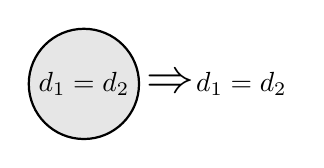
\begin{tikzpicture}[
    thick]
    \draw [fill=gray, fill opacity=0.2] (0,0) circle (.7cm);
    \draw (0,0) node {$d_1 = d_2$};
    \draw (1.1,0) node {\LARGE$\Rightarrow$};
    \draw (2,0) node {$d_1 = d_2$};
\end{tikzpicture}
      \caption{No Duplicates Rule}
    \end{subfigure}%
    \begin{subfigure}{.22\textwidth}
\vspace*{2.5em}
      \centering
\def\firstcircle{(0,0) circle (.7cm)}
\def\secondcircle{(.7,0) circle (.7cm)}
\begin{tikzpicture}[thick]
\begin{scope}
        \clip \firstcircle;
        \fill[fill=gray, fill opacity=0.9] \secondcircle;
\end{scope}
    \draw [fill=gray, fill opacity=0.6] \firstcircle;
    \draw (-0.3,0) node {$d_1$};
    \draw [fill=gray, fill opacity=0.2] \secondcircle;
    \draw (1.0,0) node {$d_2$};
    \draw (0.35,0) node {$d_3$};
\end{tikzpicture}
      \caption{Meet Rule}
    \end{subfigure}
    \begin{subfigure}{.5\textwidth}
	  \centering
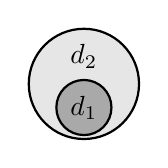
\begin{tikzpicture}[thick]
    \draw [fill=gray, fill opacity=0.2] (0,0) circle (.7cm);
    \draw [fill=gray, fill opacity=0.6] (0,-0.3) circle (.35cm);
    \draw (0,0.35) node {$d_2$};
    \draw (0,-0.3) node {$d_1$};
\end{tikzpicture}
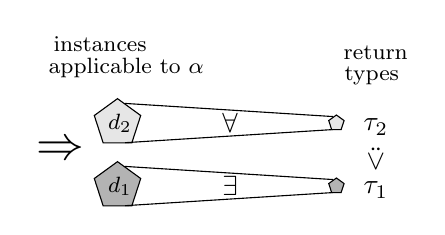
\begin{tikzpicture}[thick]
    \draw (0,.45) node {\LARGE$\Rightarrow$};
\begin{pgflowlevelscope}{\pgftransformscale{.5}}
\node[fill=gray,fill opacity=0.2,draw,regular polygon,regular polygon sides=5,xshift=1.44cm,yshift=1.6cm,minimum size=12.4mm,outer sep=0] {};
\node[opacity=0,draw,circle,xshift=1.6cm,yshift=1.6cm,minimum size=10mm,outer sep=0] (bigtop) {};
\node[fill=gray,fill opacity=0.2,draw,regular polygon,regular polygon sides=5,yshift=1.6cm,xshift=7.0cm,minimum size=.5mm,outer sep=0] (smalltop) {};
\node[opacity=0,draw,circle,yshift=1.6cm,xshift=6.9cm,minimum size=1.0mm,outer sep=0] (smalltop) {};
\draw (tangent cs:node=bigtop,point={(smalltop.south)},solution=2) -- (tangent cs:node=smalltop,point={(bigtop.south)});
\draw (tangent cs:node=bigtop,point={(smalltop.north)},solution=1) -- (tangent cs:node=smalltop,point={(bigtop.north)},solution=2);
\end{pgflowlevelscope}
    \draw (0.5,1.8) node {{\footnotesize instances}};
    \draw (.83,1.5) node {{\footnotesize applicable to $\alpha$}};
    \draw (2.15,0.8) node {$\forall$};
    \draw (2.15,0.0) node {$\exists$};
    \draw (4.0,1.7) node {{\footnotesize return}};
    \draw (3.95,1.4) node {{\footnotesize types}};
    \draw (4.0,0.75) node {$\tau_2$};
    \draw (4.0,0.35) node {$\ddot{\vee}$};
    \draw (4.0,-0.05) node {$\tau_1$};
\begin{pgflowlevelscope}{\pgftransformscale{.5}}
\node[fill=gray, fill opacity=0.6,draw,regular polygon,regular polygon sides=5,xshift=1.44cm,minimum size=12.4mm,outer sep=0] {};
\node[opacity=0,draw,circle,minimum size=10mm,xshift=1.6cm,outer sep=0] (big) {};
\node[fill=gray,fill opacity=0.6,draw,draw,regular polygon,regular polygon sides=5,xshift=7.0cm,minimum size=1mm,outer sep=0] {};
\node[opacity=0.0,draw,circle,xshift=6.9cm,minimum size=1mm,outer sep=0] (small) {};
\draw (tangent cs:node=big,point={(small.south)},solution=2) -- (tangent cs:node=small,point={(big.south)});
\draw (tangent cs:node=big,point={(small.north)},solution=1) -- (tangent cs:node=small,point={(big.north)},solution=2);
\end{pgflowlevelscope}
    \draw (.75,0.8) node {{\footnotesize $d_2$}};
    \draw (0.75,0.0) node {{\footnotesize $d_1$}};
\end{tikzpicture}
	  \caption{Return Type Rule}
	\end{subfigure}
    \caption{Overloading rules for multiple inheritance and generics
where circles denote applicable sets of generic method declarations
and pentagons denote instantiated method declarations}
    \label{fig:overloading}
\end{figure}

The overloading rules of FGF require every pair in a set of
overloaded method declarations to satisfy \emph{all} of the following
rules as illustrated in Figure~\ref{fig:overloading}:
\begin{description}
\item[\textbf{No Duplicates Rule:}]
Distinct method declarations
must have different applicable sets
(there must be some argument type $\alpha$ for which one method is applicable and the other is not).

\item[\textbf{Meet Rule:}] Let $\mathcal{S}$ be the intersection of the applicable sets of the two method declarations;
if $\mathcal{S}$ is not empty, then the overloaded set must contain a method declaration
(not necessarily distinct from the two given method declarations) whose applicable set is precisely $\mathcal{S}$.

\item[\textbf{Return Type Rule:}] If one method declaration $d_1$ is
more specific than $d_2$, for any non-$\Bottom$ type $\alpha$ in the
applicable set of $d_1$, the return type of an instance of $d_2$ that is
applicable to $\alpha$ must be a supertype of the return type of
some instance of $d_1$ that is applicable to $\alpha$.
\end{description}

Let us revisit the above ambiguous $\mbox{\textit{sort}}$ example
with an additional method declaration:
\[\begin{array}[ht]{r@{\qquad}l}
d_1:&\mbox{\textit{sort}}\ob{P \extends A}(x \COLON \kwd{List^I}\ob{P}) \COLON \kwd{SortedList^I}\ob{P} = \cdots\\
d_2:&\mbox{\textit{sort}}\ob{P \extends B}(x \COLON \kwd{List^I}\ob{P}) \COLON \kwd{SortedList^I}\ob{P} = \cdots\\
d_3:&\mbox{\textit{sort}}\ob{P \extends C}(x \COLON \kwd{List^I}\ob{P}) \COLON \kwd{SortedList^I}\ob{P} = \cdots\\
\end{array}\]
% This set of overloaded method declarations is valid since every pair
% satisfies all of the above overloading rules.
This set of overloaded method declarations is valid.
For all pairs, the No Duplicates Rule is trivially satisfied.
In the case of $d_1$ and
$d_2$, the Meet Rule is satisfied
% by $d_3$ being the meet of this pair,
($d_3$ is their meet),
and the Return Type Rule is vacuously satisfied since neither is more specific than the other.
% In the case of
For
$d_1$ and $d_3$, the Meet Rule is satisfied with $d_3$ itself as the meet; to see that
the Return Type Rule is satisfied, note that $\kwd{List^I}$ is an invariant
type constructor since FGF does not support variance.  For any
$\kwd{List^I}\ob{X}$ in the applicable set of $d_3$, there is exactly one instance
of $d_1$ (with $X$ substituted for $P$) applicable to it:
\begin{center}
$\mbox{\textit{sort}}(x \COLON \kwd{List^I}\ob{X}) \COLON \kwd{SortedList^I}\ob{X} = \cdots$.
\end{center}
Since the return type of this instance equals the return type of the corresponding instance of $d_3$: 
\begin{center}
$\mbox{\textit{sort}}(x \COLON \kwd{List^I}\ob{X}) \COLON \kwd{SortedList^I}\ob{X} = \cdots$,
\end{center}
$d_1$ and $d_3$ satisfy the Return Type Rule.  Similarly, $d_2$ and $d_3$
also satisfy all of the overloading rules.

Again, the overloading rules ensure that there is no ambiguous method
calls at run time, and that types are preserved.  In FGF, No Duplicates
Rule rules out the trivial ambiguous calls with duplicate declarations.
Meet Rule plays an important role for ensuring the existence of a
disambiguating method declaration, and Return Type Rule serves a key
role for type preservation.


\subsection{Overloading Rules for Multiple Inheritance and Generics with Variance}
\label{sec:motiv:fgfv}
Variance, as well as symmetric multiple dispatch, multiple inheritance,
and generics, may cause ambiguous method calls that cannot be resolved
at run time.  We revisit the ambiguous $\mbox{\textit{sort}}$ example in
Section~\ref{sec:motiv:fgf}.  This time, we define the same method
in a simpler way using covariant definitions of $\kwd{List^C}$ and $\kwd{SortedList^C}$.
Consider the following overloaded method declarations of $\mbox{\textit{sort}}$:
\[\begin{array}[ht]{r@{\qquad}l}
d_1:&\mbox{\textit{sort}}(x \COLON \kwd{List^C}\ob{A}) \COLON \kwd{SortedList^C}\ob{A} = \cdots\\
d_2:&\mbox{\textit{sort}}(x \COLON \kwd{List^C}\ob{B}) \COLON \kwd{SortedList^C}\ob{B} = \cdots\\
\end{array}\]
Similarly to the example in Section~\ref{sec:motiv:fgf}, for a method invocation
$\mbox{\textit{sort}}(l)$ where the run-time type of $l$ is $\kwd{List^C}\ob{C}$,
it is ambiguous which declaration to invoke: both $d_1$ and
$d_2$ are applicable to $l$ and neither is more specific than the other.
In order to ensure that there is no ambiguous method calls for
$\mbox{\textit{sort}}$ at run time, we need to add a disambiguating method
declaration $d_3$:
\[\begin{array}[ht]{r@{\qquad}l}
d_3:&\mbox{\textit{sort}}(x \COLON \kwd{List^C}\ob{C}) \COLON \kwd{SortedList^C}\ob{C} = \cdots\\
\end{array}\]
with a more specific return type than those of $d_1$ and $d_2$ for type
preservation.
% Thus, overloading rules should consider generic types with variance as well to avoid any unambiguous method calls at run time.

Variance also adds complications in type-sound dynamic dispatch.  Let us now
assume that $\kwd{List^C}$ is covariant in its type argument but
$\kwd{SortedList^I}$ is invariant.
Then, the set of three method declarations above
replacing $\kwd{SortedList^C}$ with $\kwd{SortedList^I}$ would be invalid,
because the return type $\kwd{SortedList^I}\ob{A}$ of $d_1$ would not be a supertype of the return type $\kwd{SortedList^I}\ob{C}$ of $d_3$.

Supporting variance in a type-sound manner requires keeping
track of the static types of method invocations at run time.
Let us again assume that $\kwd{List^C}$ is covariant but $\kwd{SortedList^I}$ is invariant,
and consider the following overloaded set (note that $d_3$ now has a type parameter $P$):
\[\begin{array}[ht]{r@{\qquad}r}
d_1:&\mbox{\textit{sort}}(x \COLON \kwd{List^C}\ob{A}) \COLON \kwd{SortedList^I}\ob{A} = \cdots\\
d_2:&\mbox{\textit{sort}}(x \COLON \kwd{List^C}\ob{B}) \COLON \kwd{SortedList^I}\ob{B} = \cdots\\
d_3:&\mbox{\textit{sort}}\ob{P}(x \COLON \kwd{List^C}\ob{C}) \COLON \kwd{SortedList^I}\ob{P} = \cdots\\
\end{array}\]
as well as the following generic method declaration of $\mbox{\textit{merge}}$:
\begin{center}
$\mbox{\textit{merge}}\ob{P}(x \COLON \kwd{SortedList^I}\ob{P}, y \COLON \kwd{SortedList^I}\ob{P}) \COLON \kwd{SortedList^I}\ob{P} = \cdots$
\end{center}
For a method invocation
$\mbox{\textit{merge}}(\mbox{\textit{sort}}(l_1), \mbox{\textit{sort}}(l_2))$
where the static types of $l_1$ and $l_2$ are both $\kwd{List^C}\ob{A}$ and
their run-time types are $\kwd{List^C}\ob{A}$ and $\kwd{List^C}\ob{C}$, respectively,
at compile time, both method invocations $\mbox{\textit{sort}}(l_1)$ and
$\mbox{\textit{sort}}(l_2)$ choose $d_1$ and their static types are both
$\kwd{SortedList^I}\ob{A}$.  Thus, the above $\mbox{\textit{merge}}$ call
statically invokes the following instance of the generic
$\mbox{\textit{merge}}$ declaration:
\begin{center}
$\mbox{\textit{merge}}(x \COLON \kwd{SortedList^I}\ob{A}, y \COLON \kwd{SortedList^I}\ob{A}) \COLON \kwd{SortedList^I}\ob{A}$
\end{center}
that is applicable to $\tuple{\kwd{SortedList^I}\ob{A}, \kwd{SortedList^I}\ob{A}}$.
However, at run time, while $\mbox{\textit{sort}}(l_1)$ chooses $d_1$ and
its return type is $\kwd{SortedList^I}\ob{A}$, $\mbox{\textit{sort}}(l_2)$
chooses $d_3$ and its return type depends on what actual type is inferred at run time for the type parameter $P$.
If the dynamic type inference algorithm instantiates $P$ as $A$,
$\mbox{\textit{sort}}(l_2)$ has type $\kwd{SortedList^I}\ob{A}$, which is
type sound.  But it could equally plausibly instantiate $P$ as some other type $T$,
and then no dynamic instance of the generic $\mbox{\textit{merge}}$
declaration would be applicable to 
$\tuple{\kwd{SortedList^I}\ob{A}, \kwd{SortedList^I}\ob{T}}$.
Hence, the $\mbox{\textit{merge}}$ call would fail, despite the fact that
the program successfully passed static type checking.
In order to help run-time type inference
algorithms make type-sound choices of type arguments, the language
semantics needs to make the static types of method invocations available at run time.

In this paper, we present FGFV, which sheds light on the long-standing
endeavor to support strong types, symmetric multiple dispatch, multiple inheritance,
and parametric polymorphism with variance.
% Unlike existing approaches, FGFV captures only the core language features
% to address the problem, we formally define the FGFV calculus from its
% syntax, static semantics, and dynamic semantics, and we finally prove its
% type soundness.
We formalize the static overloading rules for FGFV using
existential types and universal types quantified over method type
parameters, and design a new dynamic dispatch algorithm that is proven
type-sound to guarantee unambiguous method calls and type preservation
at run time.


\section{Language}\label{sec:lang}
In this section, we define the abstract syntax of FGFV and its well-formedness requirements.

\subsection{Notation}

Following, for example, \citet{vytiniotis13} and \citet{coughlin14}, we use an overline above mathematical material to
indicate an appropriately punctuated sequence of zero or more repetitions of the material, with a subscript added
to each metavariable in the material. Thus $\set{\rep{\alpha}}$ is equal to $\set{\alpha_1,\alpha_2,\ldots,\alpha_n}$.
Sometimes we write $\bullet$ as an explicit indication of an empty sequence.
Overlines may be nested, in which case they are expanded outermost first, so
``$\bigobb{\lobindup{\rep{\zeta}}{Q}{\rep{\xi}}}$'' expands first to
``$\bigob{\lobindup{\rep{\zeta_1}}{Q_1}{\rep{\xi_1}},\lobindup{\rep{\zeta_2}}{Q_2}{\rep{\xi_2}},\ldots,\lobindup{\rep{\zeta_n}}{Q_n}{\rep{\xi_n}}}$''
and then to
\newcommand\subfixup[1]{{\setbox0\hbox{$\scriptstyle 2$}\hbox to \wd0{$\scriptstyle #1$\hss}}}
\newcommand\subsubfixup[1]{{\setbox0\hbox{$\scriptscriptstyle 2$}\hbox to \wd0{$\scriptscriptstyle #1$\hss}}}
$$\begin{array}{@{}r@{}l@{}}
{\llbracket\;}&\bd{\zeta_{1\,1},\zeta_{1\,2},\ldots,\zeta_{1\,k_1}}\extends{Q_1}\extends\bd{\xi_{1\,1},\xi_{1\,2},\ldots,\xi_{1\,m_1}}, \\
         &\bd{\zeta_{2\,1},\zeta_{2\,2},\ldots,\zeta_{2\,k_2}}\extends{Q_2}\extends\bd{\xi_{2\,1},\xi_{2\,2},\ldots,\xi_{2\,m_2}}, \\
         &\ldots, \\
         &\bd{\zeta_{\subfixup{n}\,1},\zeta_{\subfixup{n}\,2},\ldots,\zeta_{\subfixup{n}\,k_{\subsubfixup{n}}}}\extends{Q_\subfixup{n}}\extends\bd{\xi_{\subfixup{n}\,1},\xi_{\subfixup{n}\,2},\ldots,\xi_{\subfixup{n}\,m_{\subsubfixup{n}}}}\;\rrbracket
\end{array}$$
(conceptually all on one line, broken here for reasons of space).
The copies of each inner overline expand independently, so the sequences into which they expand may have different lengths; thus
``$\bigobb{\lobindup{\rep{\zeta}}{Q}{\rep{\xi}}}$'' could expand into, e.g.,
``$\llbracket\bd{\zeta_{1\,1},\zeta_{1\,2}}\extends{Q_1}\extends\bd{\xi_{1\,1}},
         \bd{}\extends{Q_2}\extends\bd{\xi_{2\,1},\xi_{2\,2},\xi_{2\,3}}\rrbracket$''.

\newcommand\declsep{\hskip 1.5em}
Following a suggestion of Steele~\citeyearpar[0:59:37]{NEW-OLD-LANGUAGE},
we use an underline below submaterial within overlined material to prevent an 
overline from attaching subscripts to the metavariables in the submaterial;
the effect is to require the underlined material to be the same in each copy.
Thus ``$\rep{\jwfdecl[\same{\Delta}]{\psi}}$'' represents the sequence
``$\jwfdecl[\Delta]{\psi_1}\declsep\jwfdecl[\Delta]{\psi_2}\declsep\cdots\declsep\jwfdecl[\Delta]{\psi_n}$''
for any $n \geq 0$.  Similarly
$\rep{\rep{\jwftype[\same{\same{\Delta'}}]{\xi}}}$ expands to
``$\rep{\jwftype[\same{\Delta'}]{\xi_1}}\declsep\rep{\jwftype[\same{\Delta'}]{\xi_2}}\declsep\cdots\declsep\rep{\jwftype[\same{\Delta'}]{\xi_n}}$''
and then to
$$\begin{array}{@{}l@{\declsep}l@{\declsep}l@{\declsep}l@{}}
\jwftype[\Delta']{\xi_{1\,1}}&\jwftype[\Delta']{\xi_{1\,2}}&\cdots&\jwftype[\Delta']{\xi_{1\,m_1}} \\
\jwftype[\Delta']{\xi_{2\,1}}&\jwftype[\Delta']{\xi_{2\,2}}&\cdots&\jwftype[\Delta']{\xi_{2\,m_2}} \\
\ldots \\
\jwftype[\Delta']{\xi_{\subfixup{n}\,1}}&\jwftype[\Delta']{\xi_{\subfixup{n}\,2}}&\cdots&\jwftype[\Delta']{\xi_{\subfixup{n}\,m_{\subsubfixup{n}}}}
\end{array}$$
The overline notation may explicitly bind index variables by using a range expression.
In such cases, the index variables may appear explicitly in the covered material,
and subscripts are not automatically attached to metavariables.  For example,
$\bigl(\rep{m(e_i)}[3\leq i\leq 6]\bigr)$ means $(m(e_3),m(e_4),m(e_5),m(e_6))$.

Metavariables are expanded \emph{after} overlines.  Multiple occurrences of a metavariable with the same
subscript(s) must have the same expansion, but occurrences of a metavariable with different subscript(s)
may be expanded independently.  Thus ``$\bigobb{\lobindup{\rep{\zeta}}{Q}{\rep{\xi}}}$'' might ultimately expand into, e.g.,
``$\llbracket\bd{\TYP{A},\TYP{B}}\extends{\TYP{U}}\extends\bd{\TYP{List}\ob{\TYP{Boolean}}},
         \bd{}\extends{\TYP{V}}\extends\bd{\Any,\TYP{C},\TYP{Number}}\rrbracket$''.

We use horizontal lines as overlines and underlines, but also in the usual Gentzen notation
for inference rules, with premises above the line and the conclusion below.
To help reduce confusion: (1)~we use a slightly heavier and wider line for inference rules;
(2)~the line for inference rules has more space above and below it;
(3)~we do not use the inference rule notation for axioms (rules that have no premises); and
(4)~we do not nest the inference rule notation to present derivation trees.



\subsection{Syntax}\label{sec:grammar}
\begin{figure}[t]
\leavevmode
\small
\begin{array}[t]{lrll@{\hskip1ex}l}
\desc{Program} &\Pi      & ::= &  \multicolumn{2}{l}{\rep{\psi}, e}\\
\desc{Class declaration} &\psi     & ::= &  \multicolumn{2}{l}{\traitdecl{T}{\rep{V\;\beta}}{\rep{t}}{\rep{\mu}}                     
~\mid~\objectdecl{O}{\rep{\beta}}{\rep{x\COLON \tau}}{\rep{t}}{\rep{\mu}}}\\
\desc{Method definition} &\mu      & ::= &  \multicolumn{2}{l}{\methoddef{m}{\rep{\kappa}}{\rep{x\COLON\tau}}{\tau}{e}}\\
\desc{Class type parameter binding} &\beta    & ::= &  \multicolumn{2}{l}{\bindup{P}{\rep{\tau}}}\\
\desc{Method type parameter binding} &\kappa   & ::= &  \multicolumn{2}{l}{\lobindup{\rep{\tau}}{P}{\rep{\tau}}}\\
\desc{Variance mark} &V        & ::= &  \bindco &~\mid~ \bindcontra~\mid~\bindinv\\
\desc{Expression} &e      & ::= &  z
&~\mid~ ((\bar{x\COLON\tau})\COLON\tau \Rightarrow e)
~\mid~ e\apply(\bar{e})
~\mid~  O\obb{\tau}(\bar{e})
~\mid~  e.m(\rep{e})\\
\desc{Bindable variable} &z        & ::= &  x &~\mid~ \kwd{self}\\
\desc{Type} &\tau & ::= &  P
&~\mid~ c
~\mid~(\rep{\tau})
~\mid~\arrowtype{\tau}{\tau}
~\mid~\Any\\
\desc{Constructed type} &c        & ::= &  t
&~\mid~O\obb{\tau}\\
\desc{Trait type} &t        & ::= &  \multicolumn{2}{l}{T\obb{\tau}}
\end{array}
\vspace*{-.5em}
\caption{Abstract syntax of FGFV}
\label{fig:grammar}
\end{figure}

Figure~\ref{fig:grammar} shows the syntax of the FGFV calculus.
Metavariables $T$ and $U$ range over trait names;
$O$ ranges over object names;
$x$ ranges over variable and field names;
$z$ is either $x$ or the keyword $\KWD{self}$;
$m$ ranges over method names;
$P$, $Q$, $S$ range over type parameter names;
and $\tau$, $\omega$, $\zeta$, $\xi$ range over types.

A program consists of a sequence of class declarations and
a top-level expression.
A class is either a trait or an object;
traits are like Java interfaces that do not have any fields, and
objects are like Java final classes that cannot be extended.
A trait may have type parameters with variance annotations and
upper bounds, extend any number of other traits, and have method definitions.
An object is similar to a trait except that (1)~its type parameters do
not have variance annotations because they are always invariant, and
(2)~it may have fields, which are initialized when an object instance is
created.  When a class does not extend any trait, we omit the
empty extends clause $\extends \bigbd{}$.
When a class has no type parameters, we omit the
empty brackets; we write $T$ for $T\ob{}$.
A method may have type parameters as well, but they have both
lower and upper bounds.
We omit clauses when no bounds are specified; for example,
we write $T\ob{\bindco \; P}$ for $T\ob{\bindco \; \bindup{P}{}}$ and
$m\ob{Q,\bd{Q} \extends S}$ for $m\ob{\lobindup{}{Q}{}, \lobindup{Q}{S}{}}$.
By default, each type parameter has an upper bound $\Any$ and a
lower bound $\Bottom$, which we describe in the next subsection.

The bounds of a type parameter place restrictions on valid instantiations
of the type parameter; a valid type instantiation must be a subtype of
all its upper bounds and, at the same time, a supertype of
all its lower bounds, if any.
We write $\bindco$ for covariance, $\bindcontra$ for
contravariance, and $\bindinv$ for invariance.  As discussed in
Section~\ref{sec:motiv:fgfv}, variance annotations of type parameters define
subtype relations between different instances of a generic trait.
For example, consider the following trait declarations:\\[-.5em]
\[
\begin{array}{l}
\kwd{trait} \; U_1 \; \dontcares \; \kwd{end}\\
\kwd{trait} \; U_2 \extends \bigbd{U_1} \; \dontcares \; \kwd{end}\\
\kwd{trait} \; T \bigob{\bindco \; P, \bindcontra \; Q, \bindinv \; S} \;
\dontcares \; \kwd{end}
\end{array}
\]
where ``$\dontcares$'' denotes omitted material.
Because $U_2$ is a subtype of $U_1$,
the variance annotations of the type parameters of $T$ define
subtype relations such as $T\ob{U_2, U_1, U_1} \subtypeof T\ob{U_1, U_2, U_1}$.

\begin{figure}[t]
\small
\newjudge{Well-formed programs}{\jtype[]{\Pi}{g}}

\infrule[T-Program]
  { \Pi = \bar{\psi},e  \andalso
    \mathit{distinct}(\rep{\mathit{name}(\psi)})  \andalso
    \Delta = \setb{\psi}  \andalso
    \rep{\jwfdecl[\same{\Delta}]{\psi}}  \andalso
    \jtype[\Delta;\emptyseq]{e}{\expty{\dontcare}{g}} }
  { \jtype[]{\Pi}{g} }

\newjudge{Well-formed trait and object declarations}{\jwfdecl{\psi}}

{\showboxdepth=20\showboxbreadth=20

\infrule[D-Trait]
  { \Delta' = \Delta \cup \bigsetb{\lobindup{}{P}{\rep{\xi}}}  \andalso
    \mathit{distinct}(\rep{P})  \andalso
    \rep{\rep{\jwftype[\same{\same{\Delta'}}]{\xi}}}  \andalso
    \rep{\jwftype[\same{\Delta'}]{t}}  \\[2.5pt]
    \setb{J} = \properancestors[\Delta']{T\obb{P}}  \andalso
    \rep{\jancestormeetrule[\Delta'; \rep{J}]{J_i}{J_j}}[1 \leq i < j \leq \countofb{J}] \\[3.5pt]
    \rep{\same{T} \neq \mathit{name}(J)}  \andalso
    \rep{\jwfmeth[\same{\Delta';\kwd{self}\COLON T\bigobb{P};\rep{V\;P}}]{\mu}}  \andalso
    \setb{d} = \allvisible[\Delta']{T\obb{P}}  \\[3.5pt]
    \rep{\jnoduplicatesrule[\Delta']{d_i}{d_j}}[1 \leq i < j \leq \countofb{d}]  \andalso
    \rep{\jmethodmeetrule[\Delta']{d_i}{d_j}{\setb{d}}}[1 \leq i < j \leq \countofb{d}] \\[3pt]
    \rep{\jreturntyperule[\Delta']{d_i}{d_j}}[1 \leq i < j \leq \countofb{d}] \andalso
    \rep{\jreturntyperule[\Delta']{d_j}{d_i}}[1 \leq i < j \leq \countofb{d}]
    }
  { \jwfdecl{\traitdecl{T}{\rep{\bindup{V\;P}{\rep{\xi}}}}{\rep{t}}{\rep{\mu}}} }

}

\infrule[D-Object]
  { \Delta' = \Delta \cup \bigsetb{\lobindup{}{P}{\rep{\xi}}}  \andalso
    \mathit{distinct}(\bar{P})  \andalso
    \rep{\rep{\jwftype[\same{\same{\Delta'}}]{\xi}}}  \andalso
    \rep{\jwftype[\same{\Delta'}]{t}}  \\[2.5pt]
    \setb{J} = \properancestors[\Delta']{O\obb{P}}  \andalso
    \rep{\jancestormeetrule[\Delta'; \rep{J}]{J_i}{J_j}}[1 \leq i < j \leq \countofb{J}]  \\[3.5pt]
    \rep{\jwfmeth[\same{\Delta';\kwd{self}\COLON O\bigobb{P},\bar{x\COLON\tau};\rep{\bindinv\;P}}]{\mu}} \andalso
    \setb{d} = \allvisible[\Delta']{O\obb{P}}  \\[3.5pt]
    \rep{\jnoduplicatesrule[\Delta']{d_i}{d_j}}[1 \leq i < j \leq \countofb{d}]  \andalso
    \rep{\jmethodmeetrule[\Delta']{d_i}{d_j}{\setb{d}}}[1 \leq i < j \leq \countofb{d}] \\[3pt]
    \rep{\jreturntyperule[\Delta']{d_i}{d_j}}[1 \leq i < j \leq \countofb{d}] \andalso
    \rep{\jreturntyperule[\Delta']{d_j}{d_i}}[1 \leq i < j \leq \countofb{d}] \\[3pt]
    \jbwftype[\Delta']{\tau}  \andalso
    \mathit{distinct}(\bar{x})
    }
  { \jwfdecl{\objectdecl{O}{\rep{\bindup{P}{\rep{\xi}}}}{\rep{x\COLON\tau}}{\rep{t}}{\rep{\mu}}} }

\newjudge{Well-formed method declarations}{\jwfmeth{\mu}}

\infrule[D-Method]
  {
    \jscope{\bigobb{\lobindup{\rep{\zeta}}{Q}{\rep{\xi}}}} \andalso
    \Delta' = \Delta \cup \bigsetb{\lobindup{\rep{\zeta}}{Q}{\rep{\xi}}} \andalso
\jbbwftype[\Delta']{\zeta} \andalso
    \jbbwftype[\Delta']{\xi} \\[3pt]
    \mathit{distinct}(\bar{x})  \andalso
    \rep{\jwftype[\same{\Delta'}]{\tau}}  \andalso  \jwftype[\Delta']{\omega} \andalso
    \jtype[\Delta';\Gamma,\bar{x\COLON\tau}]{e}{\expty{\dontcare}{\rho}}  \andalso
\jsubtype[\Delta']{\rho}{\omega} \\[3pt]
    \mathit{distinct}(\bar{P},\bar{Q})  \andalso
    \rep{(V = \bindinv)\lor(\forall \T.\ (\same{\arrowtype{(\rep{\tau})}{\omega}}\neq\T\context{P}) \lor (\jcontextvar[\same{\Delta}]{\T}{V}))} }
  { \jwfmeth{\methoddef{m}{\rep{\lobindup{\rep{\zeta}}{Q}{\rep{\xi}}}}{\rep{x\COLON\tau}}{\omega}{e}} }

\vspace*{-1.5em}
\caption{Well-formed programs, class declarations, and method declarations}
\label{fig:wellformed}
\end{figure}

Expressions and types are conventional.
One can refer to a field or bound variable simply by mentioning it;
the keyword $\KWD{self}$ refers to the target object for the currently executing method.
Functions are first-class values; $((\bar{x\COLON\tau})\COLON\tau \Rightarrow e)$
is a (typed) function constructor,
and we write $e\apply(\bar{e})$ for
function calls.  An object creation $O\obb{\tau}(\bar{e})$ makes an
instance of $O$ by instantiating its type parameters with $\bar{\tau}$ and
initializing its fields with the values of $\bar{e}$.
While tuples are not first-class values in FGFV (they would be trivial to add,
but are not needed for our purposes), we use tuple types $(\rep{\tau})$
to denote the domain types of functions and methods, which may have multiple parameters.
The type $\Any$ is a supertype of every type (and $\Bottom$, used below, is a subtype of every type but is intentionally not expressible in the surface syntax).


\subsection{Well-formedness}\label{sec:wellformed}

We define well-formedness of a program and its declarations as shown in
Figure~\ref{fig:wellformed}.
A type-declaration environment $\Delta$ is a set of class declarations and
type parameter bindings, and
a variable-type environment $\Gamma$ is a sequence of bindable variables
and their types.  Checking well-formedness may introduce
\textit{internal types}:
\begin{center}
$\descsm{Internal type} \quad \alpha~::= P~\mid~C~\mid~\tupleb{\alpha}~\mid~
\arrowtype{\alpha}{\alpha}~\mid~\Any~\mid~\Bottom~\mid~
\uniontype{\alpha}{\alpha}~\mid~\intersectiontype{\alpha}{\alpha}$
\end{center}
which contain $\Bottom$, union types, and intersection types.
Type $\Bottom$ is a subtype of every type; hence, $\Any$ and $\Bottom$
are the top and bottom, respectively, of the type lattice.
Metavariables $\alpha, \gamma, \rho, \chi, \eta$ range over internal types.
We introduce metavariables $K$, $C$, $J$, and $M$,
analogous to $\kappa$, $c$, $t$, and $\mu$, respectively, where 
types $\tau$ in the latter are replaced by internal types $\alpha$ in the former.

Rule \rncite{T-Program} states that a program is well-formed
if its class declarations have distinct names and are well-formed, and
its top-level expression is well-formed.
%%% The following material has been obsoleted by new section on notation.
% We write $\emptyseq$ for an empty sequence.
% Following a suggestion of Steele~\citeyearpar[0:59:37]{NEW-OLD-LANGUAGE},
% we use
% an underline below submaterial within overlined material to prevent the 
% overline from attaching subscripts to the metavariables in the submaterial;
% hence, $\rep{\jwfdecl[\same{\Delta}]{\psi}}$ represents the sequence
% $\Delta\vdash\psi_1\, \mathsf{ok}\ \ \Delta\vdash\psi_2\, \mathsf{ok}\ \cdots\ \Delta\vdash\psi_n\, \mathsf{ok}$
% for any appropriate $n \geq 0$.
The type of a program is the type of its top-level expression;
the metavariable $g$ and $h$ represents a \textit{ground type},
which is a type that contains no type parameters.
We describe well-formedness and type checking of expressions
in Section~\ref{sec:static}.

Rules \rncite{D-Trait} and \rncite{D-Object} check well-formedness
of class declarations.  For the declaration of a class $C$,
they verify that the type parameter names of the declaration are distinct,
that the types used in the declaration are well-formed,
and that the declared methods are well-formed.
In addition, as we explain later in this subsection,
they make sure that (1)~the \textit{proper ancestors} of $C$,
which are all the traits $C$ extends, by explicitly extending and
transitively inheriting as well, are well-formed, and
(2)~the \textit{visible methods} of $C$,
which are the methods either declared by $C$ or inherited
from the traits $C$ extends, obey the overloading rules.
The only differences are that rule \rncite{D-Trait} additionally
guarantees that a trait does not extend itself, and rule \rncite{D-Object}
guarantees that the names of the fields are distinct.

Well-formedness of types is conventional
as shown in Figure~\ref{fig:wellformedtypes}.
The types $\Any$ and $\Bottom$ are trivially well-formed.
A type parameter $P$ is well-formed under a type-declaration environment
$\Delta$, if $\Delta$ contains a binding of $P$.
A constructed type $T\obb{\alpha}$ or $O\obb{\alpha}$ is well-formed, if
the trait $T$ or the object $O$ is declared in the given
type-declaration environment and all the type arguments $\rep{\alpha}$
are well-formed and satisfy the declared
bounds of their corresponding type parameters.
Finally, the remaining structural types such as tuple types, arrow types, 
union types, and intersection types are well-formed,
if all their component types are.

\begin{figure}[t]
\small
\newjudge{Well-formed types}{\jwftype{\alpha}}
\smallskip
\begin{tabular}{@{}c@{\hskip0.02\textwidth}c@{}}
\begin{minipage}[t]{0.48\textwidth}
\infax[W-Any]
  { \jwftype{\Any} }
\smallskip

\infax[W-Bottom]
  { \jwftype{\Bottom} }
\smallskip

\infrule[W-Param]
  { \lobindup{\dontcares}{P}{\dontcares} \in \Delta }
  { \jwftype{P} }
\smallskip

\infrule[W-Tuple]
  { \jbwftype{\alpha} }
  { \jwftype{(\bar{\alpha})} }

\end{minipage}&
\begin{minipage}[t]{.5\textwidth}
\infrule[W-Arrow]
  { \jwftype{\alpha}  \andalso  \jwftype{\rho} }
  { \jwftype{\arrowtype{\alpha}{\rho}} }
\smallskip

\infrule[W-Union]
  { \jwftype{\alpha}  \andalso  \jwftype{\gamma} }
  { \jwftype{\uniontype{\alpha}{\gamma}} }
\smallskip

\infrule[W-Intersection]
  { \jwftype{\alpha}  \andalso  \jwftype{\gamma} }
  { \jwftype{\intersectiontype{\alpha}{\gamma}} }
\smallskip

\end{minipage}
\end{tabular}
\infrule[W-Trait]
  { \traitdecl{T}{\rep{\bindup{V\;P}{\rep{\xi}}}}{\dontcares}{\dontcares} \in \Delta \andalso
    \jbwftype{\alpha} \andalso
    \jbsubtype{\alpha}{\same{\substb{\alpha}{P}}\bigtypeintersection\setb{\xi}} }
  { \jwftype{T\obb{\alpha}} }
\smallskip

\infrule[W-Object]
  { \objectdecl{O}{\rep{\bindup{P}{\rep{\xi}}}}{\dontcares}{\dontcares}{\dontcares} \in \Delta \andalso
    \jbwftype{\alpha} \andalso
    \jbsubtype{\alpha}{\same{\substb{\alpha}{P}}\bigtypeintersection\setb{\xi}} }
  { \jwftype{O\obb{\alpha}} }
\vspace*{-1em}
\caption{Well-formed types}
\label{fig:wellformedtypes}
\end{figure}

The proper ancestors $\setb{J}$ of a class $C$ are well-formed, if
every pair in $\setb{J}$ satisfies one of the well-formed ancestors rules
shown in Figure~\ref{fig:ancestors}: $\rep{\jancestormeetrule
[\Delta'; \rep{J}]{J_i}{J_j}}[1 \leq i < j \leq \countofb{J}]$.
The well-formed ancestors rules ensure that if a class $C$ extends
two instances of a trait $T$, $T\obb{\alpha}$ and $T\obb{\rho}$,
then $C$ also extends some $T\obb{\gamma}$
(which may be $T\obb{\alpha}$, $T\obb{\rho}$,
or a third instance) that extends both $T\obb{\alpha}$ and $T\obb{\rho}$.
Therefore, because the rules guarantee that there always exists a single
minimal ancestor when a class extends multiple instances of a trait,
no ambiguous method calls are possible due to multiple instances of a trait
as discussed in Section~\ref{sec:dynamic}.


\begin{figure}[t]
\small
\newjudge{Well-formed ancestors}{\jancestormeetrule{J}{J}}
\vspace*{-.7em}

\infrule[Anc-Diff-Trait]
  { T \neq T' }
  { \jancestormeetrule{T\obb{\alpha}}{T'\obb{\eta}} }

\vspace*{-1em}
\infrule[Anc-Same-Trait]
  { T\obb{\gamma} \in \setb{J}  \andalso
    \jsubtype{T\obb{\gamma}}{T\obb{\alpha}}  \andalso
    \jsubtype{T\obb{\gamma}}{T\obb{\eta}} }
  { \jancestormeetrule{T\obb{\alpha}}{T\obb{\eta}} }

\newjudge{Well-formed type parameter bindings}{\jscope{\obb{K}}}
\vspace*{-.7em}

\infax[Binding-Empty]
  { \jscope{\ob{}} }

\vspace*{-1.5em}
\infrule[Binding-Step]
 { \FV(\bar{\chi'})\subseteq\mathit{parameters}(\Delta)\cup\setb{P} \andalso
   \FV(\bar{\eta'})\subseteq\mathit{parameters}(\Delta) \\%[3pt]
   \jsubtype{\bigtypeunion\bigsetb{\chi'} }{ \bigtypeintersection\bigsetb{\eta'} } \andalso
   \jscope{\obb{\lobindup{\rep{\chi}}{P}{\rep{\eta}}}} }
 { \jscope{\ob{\rep{\lobindup{\rep{\chi}}{P}{\rep{\eta}}},\lobindup{\rep{\chi'}}{P'}{\rep{\eta'}}}} }

\vspace*{-1.5em}
\caption{Well-formed ancestors and type parameter bindings}
\label{fig:ancestors}
\end{figure}

The visible methods $\setb{d} = \setb{\tuple{C,M}}$ of a class 
obey the overloading rules if every pair in $\setb{d}$ satisfies 
the overloading rules described in Section~\ref{sec:rules:formal}.
The set $\setb{\tuple{C,M}}$ contains pairs of visible method declarations 
$\bar{M}$ and their defining classes $\bar{C}$.

Rule \rncite{D-Method} checks well-formedness of method declarations.
For the method declaration $\mu$, it verifies that the parameter names
of the declaration are distinct;
that the class type parameters and the method type parameters
of the declaration are collectively distinct;
that types used in the declaration are well-formed;
that the body expression is well-formed;
and that the type of the body expression is a subtype of the 
declared return type.  In addition, as we discuss below,
it checks that method type parameter bindings are well-formed and
that any references to trait type parameters are correctly used
according to their variance annotations.

A sequence of method type parameter bindings is well-formed,
if (1)~every reference to a method type parameter falls within its scope
(which extends to the right of its declaration),
(2)~no reference to a method type parameter appears in any of the upper bounds,
and (3) for each type parameter, the union of its lower bounds is a subtype
of the intersection of its upper bounds.
As we discuss in Section~\ref{sec:discuss},
restriction (1) makes dynamic dispatch more efficient
and restriction (2) makes it consistent.  Figure~\ref{fig:ancestors}
shows the rules for well-formed type parameter bindings.

Trait type parameters are correctly used according to their variance annotations,
if covariant and contravariant type parameters appear only at
covariant and contravariant positions, respectively.
In order to express this restriction, we introduce a \textit{type context} $\T$,
which defines positions where a type can appear within another type.
Similarly to the conventional evaluation contexts~\cite{wright94},
a type context $\T$ is a type with one of its components replaced by a hole,
denoted by ``$\emptycontext$''.  The type $\T\context{\tau}$ results from
placing a type $\tau$ in the hole of $\T$:
\begin{center}
$\descsm{Type context} \quad 
\T~::=~\emptycontext ~\mid~ T\ob{\bar\tau, \T, \bar\tau} ~\mid~ O\ob{\bar\tau, \T, \bar\tau} ~\mid~ \tuple{\bar\tau, \T, \bar\tau} ~\mid~ \arrowtype{\T}{\tau} ~\mid~\arrowtype{\tau}{\T}$
\end{center}
Thus, if $\tau = \arrowtype{\tuple{P,T\ob{Q}}}{\Any}$, 
then $\tau = \T\context{P} = \T'\context{Q}$ where 
$\T = \arrowtype{\tuple{\emptycontext, T\ob{Q}}}{\Any}$ and 
$\T' = \arrowtype{\tuple{P, T\ob{\emptycontext}}}{\Any}$.

\begin{figure}[t]
\small
\smallskip
\newjudge{Variance of type context}{\jcontextvar{\T}{V}}
\begin{tabular}{@{}c@{\hskip0.01\textwidth}c@{}}
\begin{minipage}[t]{0.5\textwidth}
\infax[Tc-Empty] {\jcontextvar{\emptycontext}{\bindco}}
\smallskip

\infrule[Tc-Trait]
  { \traitdecl{T}{\rep{\bindup{V\;\dontcare}{\dontcares}}}{\dontcares}{\dontcares} \in \Delta \\[3pt]
    i = \countof{\rep\tau} + 1  \andalso
    \countofb{V} = \countof{\rep\tau} + \countof{\rep\omega} + 1  \\[3pt]
    \jcontextvar{\T}{V'} \andalso
    V = V_i \times V' }
  { \jcontextvar{T\ob{\bar\tau,\T,\bar\omega}}{V} }
\smallskip

\infax[Tc-Obj] { \jcontextvar{O\ob{\bar\tau,\T,\bar\omega}}{\bindinv} }

\smallskip

\newjudge{Flip of variance}{\flip{V} = V}
\begin{equation*}
\flip{V} =
\begin{cases}
\bindcontra & \text{if } V = \bindco\\
\bindco & \text{if } V = \bindcontra\\
\bindinv & \text{if } V = \bindinv\\
\end{cases}
\end{equation*}

\end{minipage}&
\begin{minipage}[t]{.5\textwidth}
\infrule[Tc-Tuple]
  { \jcontextvar{\T}{V} }
  { \jcontextvar{(\bar\tau,\T,\bar\omega)}{V} }
\smallskip

\infrule[Tc-Arrow-Param]
  { \jcontextvar{\T}{V'}
  { \andalso V=\flip{V'} } }
  { \jcontextvar{\arrowtype{\T}{\tau}}{V} }
\smallskip

\infrule[Tc-Arrow-Return]
  { \jcontextvar{\T}{V} }
  { \jcontextvar{\arrowtype{\tau}{\T}}{V} }
\smallskip

\smallskip

\newjudge{Composition of variance}{V \times V = V}

\begin{equation*}
V_1 \times V_2 =
\begin{cases}
\bindinv & \text{if } V_1 = \bindinv \lor V_2 = \bindinv\\
\bindco & \text{if } V_1 \neq \bindinv \land V_2 \neq \bindinv \land V_1 = V_2\\
\bindcontra & \text{if } V_1 \neq \bindinv \land V_2 \neq \bindinv \land V_1 \neq V_2\\
\end{cases}
\end{equation*}

\end{minipage}
\end{tabular}
\vspace*{-1em}
\caption{Variance of type context}
\label{fig:contextvar}
\end{figure}

Using type contexts, the last premise of rule \rncite{D-Method} ensures that
the class type parameters of a method appear in correct positions.
Considering the arrow type representing the method's type
$\tau' = \arrowtype{(\rep{\tau})}{\omega}$,
an invariant type parameter can appear anywhere in $\tau'$. However, 
when a covariant or contravariant type parameter $P$ appears in 
$\tau' = \T\context{P}$, the \textit{variance of the type context} of $P$
should match the variance $V$ of $P$: $\Delta\vdash{\T}\,\mathsf{variance}\,V$.
As shown in Figure~\ref{fig:contextvar},
the variance of a type context is defined inductively:
(1)~the hole is covariant;
(2)~components of tuple types, return types of arrow types, and
covariant type parameters of traits preserve
the variance of their enclosing contexts;
(3)~parameter types of arrow types and
contravariant type parameters of traits flip
the variance of their enclosing contexts; and
(4)~type parameters of objects and
invariant type parameters of traits are invariant.
For example, if $\tau = \arrowtype{\tuple{P,T\ob{Q}}}{\Any}$
is a method's type where $P$ and $Q$ are class type parameters and
$T$ has a contravariant type parameter,
then
$P$ is required to be contravariant or invariant and $Q$ is required to be covariant or invariant.

\section{Overloading Rules}\label{sec:rules}
Now, we formalize the overloading rules informally discussed in Section~\ref{sec:motiv:fgf}
for FGFV.

\subsection{Formalization of Overloading Rules}\label{sec:rules:formal}
\begin{figure}[t]
\small
\begin{tabular}{@{}c@{\hskip0.02\textwidth}c@{}}
\begin{minipage}[t]{.48\textwidth}
\typicallabel{No-Dup-Not-Less}

\newjudge{No Duplicates Rule}{\jnoduplicatesrule{d}{d}}

\infrule[No-Dup-Triv]
  { \name{d}\not=\name{d'} }
  { \jnoduplicatesrule{d}{d'} }
\smallskip

\infrule[No-Dup-Not-Less]
  { \neg\bigtuple{\jle{\dom(d)}{\dom(d')}} }
  { \jnoduplicatesrule{d}{d'} }
\smallskip

\infrule[No-Dup-Not-Gtr]
  { \neg\bigtuple{\jle{\dom(d')}{\dom(d)}} }
  { \jnoduplicatesrule{d}{d'} }

\end{minipage}&%
\begin{minipage}[t]{.5\textwidth}

\newjudge{Meet Rule}{\jmethodmeetrule{d}{d}{\setb{d}}}

\typicallabel{Meet-Third}

\infrule[Meet-Triv]
  { \name{d}\not=\name{d'} }
  { \jmethodmeetrule{d}{d'}{\dontcare} }
\smallskip

\infrule[Meet-Excl]
  { \jle{\bigtuple{\dom(d)\existentialmeet\dom(d')}}{\existstype{\verythinmathspace}{\Bottom}} }
  { \jmethodmeetrule{d}{d'}{\dontcare} }
\smallskip

\infrule[Meet-Less]
  { \jle{\dom(d)}{\dom(d')} }
  { \jmethodmeetrule{d}{d'}{\dontcare} }
\smallskip

\infrule[Meet-Gtr]
  { \jle{\dom(d')}{\dom(d)} }
  { \jmethodmeetrule{d}{d'}{\dontcare} }
\end{minipage}
\end{tabular}

\vspace*{-.5em}
\infrule[Meet-Third]
  { d'''\in\setb{d''}  \quad
    \name{d}=\name{d'}=\name{d'''} \quad
    \jequivalent{\dom(d''')}{\bigtuple{\dom(d)\sqcap\dom(d')}} }
  { \jmethodmeetrule{d}{d'}{\setb{d''}} }

\newjudge{Return Type Rule}{\jreturntyperule{d}{d}}

\typicallabel{Return-Not-Less}

\begin{tabular}{@{}c@{\hskip0.05\textwidth}c@{}}
\begin{minipage}[t]{.45\textwidth}
\infrule[Return-Triv]
  { \name{d}\not=\name{d'} }
  { \jreturntyperule{d}{d'} }
\end{minipage}
&
\begin{minipage}[t]{.5\textwidth}
\infrule[Return-Not-Less]
  { \neg\big(\jle{\dom(d)}{\dom(d')}\big) }
  { \jreturntyperule{d}{d'} }
\end{minipage}
\end{tabular}

\infrule[Return-Test]
  { \arrow(d) = \foralltypeb{\kappa}{\arrowtype{\alpha}{\rho}}
    \qquad
    \rep{\kappa = \lobindup{\rep{\chi}}{P}{\rep{\eta}}}
    \qquad
    \arrow(d') = \foralltypeb{\kappa'}{\arrowtype{\alpha'}{\rho'}}
    \\[3pt]
    \rep{\kappa' = \lobindup{\rep{\chi'}}{Q}{\rep{\eta'}}}
    \qquad
    \mathit{distinct}(\rep{P},\rep{Q})
    \qquad
    \jle{\dom(d)}{\dom(d')}
    \\[3pt]
    \jle{\foralltypeb{\kappa}{\arrowtype{\alpha}{\rho}}}{\foralltype{\bar{\kappa},\bar{\kappa'}}{\arrowtype{\intersectiontype{\alpha}{\alpha'}}{\rho'}}} }
  { \jreturntyperule{d}{d'} }

\vspace*{-1.5em}
\caption{Overloading rules for FGFV}
\label{fig:overloadingrules}
\end{figure}

The overloading rules require that every pair in a set of overloaded method
declarations satisfies all three rules defined in Figure~\ref{fig:overloadingrules}.
To determine whether one method declaration is more specific than the other,
while the informal rules in Section~\ref{sec:motiv:fgf} used the subset relation
of their applicable sets, which is not practically checkable,
we use the subtype relation of their domain types as in \citet{oopsla11}.
Note that even though FGFV additionally supports variance annotations of
trait type parameters, the overloading rules for FGF remain the same
because covariant or contravariant types affect only the well-formedness of
method declarations rather than the validity of overloading.

If two method declarations have different names, they vacuously
satisfy all the rules ({\sc [No-Dup-Triv]}, {\sc [Meet-Triv]}, and
{\sc [Return-Triv]}).  The No Duplicates Rule also checks whether the
domain types of two declarations are different; if the domain type of one
declaration is not a subtype of the domain type of the other, they
satisfy the rule ({\sc [No-Dup-Not-Less]} and {\sc [No-Dup-Not-Gtr]}).
The Meet Rule is satisfied if two domain types exclude
each other ([{\sc Meet-Excl}]), they are in a subtype relation
({\sc [Meet-Less]} and {\sc [Meet-Gtr]}), or the domain type of a third
declaration of the same name is the intersection type of the domain types
of two declarations ({\sc [Meet-Third]}).  The Return Type Rule is
satisfied if two domain types are not in a subtype relation
({\sc [Return-Not-Less]}), or if two arrow types derived from the two declarations are
in a subtype relation ({\sc [Return-Test]}).
% We discuss the domain types
% and arrow types of method declarations and their subtype relations in
% the next subsection.

\subsection{Quantified Types}\label{sec:quant}
\begin{figure}[t]
\small
\newjudge{Well-formed substitution}{ \jobeys{\sigma}{\listofb{P}}{\listofb{\chi}}{\listofb{\eta}} }

\infrule
  { \sigma=\substb{\alpha}{P}
    \andalso
    \rep{\jsubtype[\same{\Delta}]{\same{\sigma}\chi}{\alpha}}
    \andalso
    \rep{\jsubtype[\same{\Delta}]{\alpha}{\same{\sigma}\eta}}
  }
  { \jobeys{\sigma}{\listofb{P}}{\listofb{\chi}}{\listofb{\eta}} }
\vspace*{-1em}
\caption{Well-formed substitution}
\label{fig:wellformedsubst}
\end{figure}

\begin{figure}[t]
\small
\typicallabel{x}
\newjudge{Existential inner subtyping}{\jleinnerusing{\Xi}{\Xi}{\sigma}}
\vspace*{-.5em}

\infrule[E-Sub]
  { \Delta' = \Delta \cup \setb{\lobindup{\rep{\chi}}{P}{\rep{\eta}}} \andalso
    \setb{P} \cap \FV(\rep{\rep{\chi'}},\rep{\rep{\eta'}},{\alpha'}) = \emptyset \andalso
    \sigma = \Bigsubstb{\gamma}{Q} \andalso
	\rep{\gamma\neq\Bottom} \\[3pt]
	\jobeys[\Delta']{\sigma}{\listofb{Q}}{\listofb{\bigtypeunion\setb{\chi'}}}{\listofb{\bigtypeintersection\setb{\eta'}}} \andalso
    \jsubtype[\Delta']{\alpha}{\sigma\alpha'} }
  { \jleinnerusingtight{\existstypeb{\lobindup{\rep{\chi}}{P}{\rep{\eta}}}{\alpha}}{\existstypebigb{\lobindup{\rep{\chi'}}{Q}{\rep{\eta'}}}{\alpha'}}{\sigma} }

\newjudge{Universal inner subtyping}{\jleinnerusing{\Upsilon}{\Upsilon}{\sigma}}
\vspace*{-.5em}

\infrule[U-Sub]
  { \Delta' = \Delta \cup \setb{\lobindup{\rep{\chi'}}{Q}{\rep{\eta'}}} \andalso
    \setb{Q} \cap \FV(\rep{\rep\chi},\rep{\rep\eta},{\alpha}) = \emptyset \andalso
    \sigma = \Bigsubstb{\gamma}{P} \andalso
	\rep{\gamma\neq\Bottom} \\[3pt]
	\jobeys[\Delta']{\sigma}{\listofb{P}}{\listofb{\bigtypeunion\setb{\chi}}}{\listofb{\bigtypeintersection\setb{\eta}}} \andalso
    \jsubtype[\Delta']{\sigma\alpha}{\alpha'} }
  { \jleinnerusingtight{\foralltypebigb{\lobindup{\rep{\chi}}{P}{\rep{\eta}}}{\alpha}}{\foralltypeb{\lobindup{\rep{\chi'}}{Q}{\rep{\eta'}}}{\alpha'}}{\sigma} }

\newjudge{Intersection of existential types}{\Xi\existentialmeet\Xi}
\vspace*{-.5em}
\infrule
  { \mathit{distinct}(\bar{P},\bar{P'}) \andalso
    \setb{P'}\cap\FV(\rep{\rep\chi},\rep{\rep\eta},\alpha)=\setb{P}\cap\FV(\rep{\rep{\chi'}},\rep{\rep{\eta'}},\alpha')=\emptyset }
  { \Bigtuple{\existstypeb{\lobindup{\rep{\chi}}{P}{\rep{\eta}}}{\alpha}} \existentialmeet \Bigtuple{\existstypeb{\lobindup{\rep{\chi'}}{P'}{\rep{\eta'}}}{\alpha'}} = 
    \existstype{\bar{\lobindup{\rep{\chi}}{P}{\rep{\eta}}},\bar{\lobindup{\rep{\chi'}}{P'}{\rep{\eta'}}}}{\intersectiontype{\alpha}{\alpha'}} }

\newjudge{Existential reduction}{\jtreds{\Xi}{\Xi}{\sigma}}
\vspace*{.5em}

\begin{tabular}{@{}c@{\hskip0.05\textwidth}c@{}}
\begin{minipage}[t]{.55\textwidth}
\infrule
  {\jcnequiv{\alpha}{\Bottom}{\mathcal{C}} \andalso \toConstraint{\setb{K}}{\mathcal{C}'} \\
   \junify{\mathcal{C} \wedge \mathcal{C}'}{\sigma}{\mathcal{C}''} \andalso \toBounds{\mathcal{C}''}{\setb{K'}}}
  {\jtreds{\existstypeb{K}{\alpha}}{\existstypeb{K'}{\sigma\alpha}}{\sigma}}
\end{minipage}
&
\begin{minipage}[t]{.4\textwidth}
\infrule
  {\text{otherwise}}
  {\jtreds{\existstypeb{K}{\alpha}}{\existstypeb{K}{\alpha}}{\emptysubst}}
\end{minipage}
\end{tabular}
\bigskip

\newjudge{Universal reduction}{\jtreds{\Upsilon}{\Upsilon}{\sigma}}

\vspace*{-2em}
\hspace*{18em}
\begin{minipage}[t]{.5\textwidth}
\infrule
  { \jtreds{\existstypeb{K}{\alpha}}{\existstypeb{K'}{\alpha'}}{\sigma} }
  { \jtreds{\foralltypeb{K}{\arrowtype{\alpha}{\omega}}}{\foralltypeb{K'}{\arrowtype{\alpha'}{\sigma\omega}}}{\sigma} }
\end{minipage}
\bigskip

\newjudge{Existential subtyping}{\jleusing{\Xi}{\Xi}{\sigma} \andalso \jle{\Xi}{\Xi}}

\begin{tabular}{@{}c@{\hskip0.05\textwidth}c@{}}
\begin{minipage}[t]{.55\textwidth}
\infrule
  { \jtreds{\Xi}{\Xi''}{\dontcare} \andalso \jleinnerusing{\Xi''}{\Xi'}{\sigma} }
  { \jleusing{\Xi}{\Xi'}{\sigma} }
\end{minipage}
&
\begin{minipage}[t]{.4\textwidth}
\infrule
  { \jleusing{\Xi}{\Xi'}{\dontcare} }
  { \jle{\Xi}{\Xi'} }
\end{minipage}
\end{tabular}
\medskip

\newjudge{Universal subtyping}{\jleusing{\Upsilon}{\Upsilon}{\sigma} \andalso \jle{\Upsilon}{\Upsilon}}

\begin{tabular}{@{}c@{\hskip0.05\textwidth}c@{}}
\begin{minipage}[t]{.55\textwidth}
\infrule
  { 
\jtreds{\Upsilon'}{\Upsilon''}{\dontcare}
\andalso 
\jleinnerusing{\Upsilon}{\Upsilon''}{\sigma} 
 }
  { \jleusing{\Upsilon}{\Upsilon'}{\sigma} }
\end{minipage}
&
\begin{minipage}[t]{.4\textwidth}
\infrule
  { \jleusing{\Upsilon}{\Upsilon'}{\dontcare} }
  { \jle{\Upsilon}{\Upsilon'} }
\end{minipage}
\end{tabular}

\smallskip
\newjudge{Constraint solving}{\junify{\C}{\sigma}{\C}}

\smallskip
\newjudge{Conversion of type environment to constraints}{\toConstraint{\Delta}{\C}}

\smallskip
\newjudge{Conversion of constraints to type environment}{\toBounds{\C}{\Delta}}

\vspace*{-.5em}
\caption{Subtype relations of quantified types}
\label{fig:quantified}
\end{figure}

As proposed by \citet{bm97}, we represent domain types and arrow types
of generic method declarations as existential types $\Xi$ and universal
types $\Upsilon$, respectively, collectively called \emph{quantified types}.
For presentation brevity, we omit $C$ from $d = (C, M)$ where a method declaration
$M = \methoddef{m}{\rep{K}}{\rep{x\COLON\alpha}}{\rho}{e}$ is declared in
a class $C$.
The domain type of $d$ is $\dom(d) =
\existstypebigb{K}{\tuple{\bar{\alpha}}}$ and its arrow type is
$\arrow(d) = \foralltypebigb{K}{\arrowtype{\tuple{\bar{\alpha}}}{\rho}}$.
% Because we compare domain types to see whether one generic method
% declaration is more specific than the other, which amounts to see whether
% any instance of the former is more specific than an instance of the latter,
% an existential type $\existstypebigb{K}{\alpha}$ is a subtype of the other
% existential type $\existstypebigb{K'}{\alpha'}$ if there exists
% a substitution $\sigma$ for the type parameters bound in $\rep{K'}$ that makes
% $\sigma\alpha'$ a supertype of $\alpha$.
We compare domain types to decide whether one generic method
declaration is more specific than the other;
an existential type $\existstypebigb{K}{\alpha}$ is a subtype of another
existential type $\existstypebigb{K'}{\alpha'}$ if there exists
a well-formed substitution $\sigma$ for the type parameters bound in $\rep{K'}$ that makes
$\sigma\alpha'$ a supertype of $\alpha$.
A substitution is well-formed if it satisfies the bounds of type parameters
as shown in Figure~\ref{fig:wellformedsubst}.
In contrast, we compare arrow types to see whether the return type
of a more specific generic method declaration can be a subtype of the return
type of a less specific one;
a universal type $\foralltypebigb{K}{\alpha}$ is a subtype of the other
universal type $\foralltypebigb{K'}{\alpha'}$ if there exists
a well-formed substitution $\sigma$ for the type parameters bound in $\rep{K}$ that
makes $\sigma\alpha$ a subtype of $\alpha'$.
Figure~\ref{fig:quantified} formally defines these ``inner'' subtyping
rules for quantified types.  (We assume the usual conventions about
using $\alpha$-conversion to rename bound variables when necessary
to satisfy premises that require variable names to be distinct.)
Finally, the intersection type of two
existential types $\existstypebigb{K}{\alpha}$ and
$\existstypebigb{K'}{\alpha'}$ used in [{\sc Meet-Excl}] and [{\sc Meet-Third}] is
$\exists{\big\llbracket\verythinmathspace \bar{K},\bar{K'} \verythinmathspace\big\rrbracket}{\intersectiontype{\alpha}{\alpha'}}$,
because whenever both $\sigma\alpha$ and $\sigma'\alpha'$ are supertypes
of a type $\tau$ for some $\sigma$ and $\sigma'$,
$(\sigma\compose\sigma')\intersectiontype{\alpha}{\alpha'}$ is a supertype of
$\tau$ as well.

While the subtype relation of domain types is a sound
approximation of the subset relation of applicable sets, it is not
complete; when the applicable set of one declaration is a subset
of that of the other, their domain types may not be in a subtype relation.
Consider the following:
\[
\begin{array}{l}
m\ob{P}(x:{\sf ArrayList}\ob{P})\ \dontcare\andalso
m\ob{Q\extends T}(y:{\sf List}\ob{Q})\ \dontcare\andalso
m\ob{R\extends T}(z:{\sf ArrayList}\ob{R})\ \dontcare
\end{array}
\]
for some trait $T$ where ${\sf ArrayList}$ extends ${\sf List}$ and both
are invariant, and call them $d_1$, $d_2$, and $d_3$ in order.
Even though they are a valid overloading because the applicable set of
$d_3$ is the intersection of those of $d_1$ and $d_2$,
the intersection of the two domain types
$\Xi_{\sqcap}=\existstype{P,Q\extends T}{\intersectiontype{{\sf ArrayList}\ob{P}}{{\sf List}\ob{Q}}}$
is not a subtype of the domain type of $d_3$, 
$\Xi_3=\existstype{R\extends T}{{\sf ArrayList}\ob{R}}$.
However, because ${\sf ArrayList}$ extends ${\sf List}$ and both are
invariant, any subtypes of theirs are exclusive unless they are both
${\sf ArrayList}\ob{S}$ for some type $S$ that is a subtype of $T$.
Thus, $\Xi_{\sqcap}$ denotes the same applicable set as
$\existstype{S\extends T}{{\sf ArrayList}\ob{S}}$, which is
a subtype of $\Xi_3$ using $\subst{R}{S}$.


Therefore, in order to reduce the gap between the subset relation of
applicable sets and the subtype relation of domain types,
we extend the subtype relation of existential types using
\emph{existential reduction}.  As defined in Figure~\ref{fig:quantified},
existential reduction infers a simplified existential type from a given
existential type $\existstype{\rep{K}}{\alpha}$.
As defined in Figure~\ref{fig:constraints}, it first collects
constraints $\C$ that make $\alpha$ different from $\Bottom$:
${\Delta}\turnstile{\alpha}\,{\not\equiv}\,{\Bottom}\Rightarrow{\C}$.
It then tries to find types that instantiate the type parameters bound in
$\rep{K}$ or simply collects their bounds by solving $\C$ and the
constraints on the type parameters; it makes a substitution $\sigma$
for the type parameters that have types to instantiate with and
constraints $\C''$ for the type parameters that have only bounds.
Using the substitution $\sigma$ and type parameter bindings $\rep{K'}$
generated from $\C''$, it produces a simplified existential type
$\existstype{\rep{K'}}{\sigma\alpha}$.  Finally, in the extended subtype
relation, one existential type is a subtype of the other if a reduced
existential type of the former is a subtype of the latter
by the inner subtyping rule as shown in Figure~\ref{fig:quantified}.

\begin{figure}[t]
\small
\begin{tabular}{@{}l@{}l@{}}
\begin{minipage}[t]{.4\textwidth}
\textbf{Constraint grammar} \par
\smallskip
\noindent\(
\begin{array}{@{}lclcl@{}}
\C &::=& \FALSE &\mid& \TRUE \\
  &\mid& T <: T &\mid& T \exc T \\
  &\mid& T \not<: T &\mid& T \nexc T \\
  &\mid& \C \wedge \C &\mid& \C \vee \C \\
  \end{array}
\)
\end{minipage}
&
\hspace*{-1em}
\begin{minipage}[t]{0.6\textwidth}
\newjudge{Constraint negation}{\neg \C = \C}
\noindent\(
\begin{array}{@{}l@{\hspace{1ex}}c@{\hspace{1ex}}ll@{\hspace{1ex}}c@{\hspace{1ex}}l@{}}
\neg(\FALSE) &=& \TRUE & \neg(\TRUE) &=& \FALSE \\
\neg(T \subtypeof T') &=& T \nsubtypeof T' & \neg(T \exc T') &=& T \nexc T'\\
\neg(T \nsubtypeof T') &=& T \subtypeof T' & \neg(T \nexc T') &=& T \exc T' \\
\neg(\C \wedge \C) &=& \neg(\C) \vee \neg(\C) & \neg(\C \vee \C) &=& \neg(\C) \wedge \neg(\C) \\
\end{array}
\)
\end{minipage}\\

\begin{minipage}[t]{0.5\textwidth}
\newjudge{Conditional non-subtyping}{\jnsub{\alpha}{\alpha}{\C}}

\infrule
  { \jsub{\alpha}{\eta}{\C} }
  { \jnsub{\alpha}{\eta}{\neg\C} }

\newjudge{Conditional equivalence}{
\begin{tabular}{l}
\jequiv{\alpha}{\alpha}{\C}\\
\jnequiv{\alpha}{\alpha}{\C}
\end{tabular}
}

\infrule
  { \jsub{\alpha}{\eta}{\C} \andalso \jsub{\eta}{\alpha}{\C'} }
  { \jequiv{\alpha}{\eta}{\C \wedge \C'} }

\medskip
\infrule
  { \jequiv{\alpha}{\eta}{\C} }
  { \jnequiv{\alpha}{\eta}{\neg\C} }

\end{minipage}
&
\begin{minipage}[t]{.5\textwidth}
\newjudge{Conditional variance test}{\jcomp{\alpha}{\alpha}{V}{\C}}

\infrule
  { \jsub{\alpha}{\eta}{\C} }
  { \jcomp{\alpha}{\eta}{\bindco}{\C} }

\infrule
  { \jsub{\eta}{\alpha}{\C} }
  { \jcomp{\alpha}{\eta}{\bindcontra}{\C} }

\infrule
  { \jequiv{\alpha}{\eta}{\C} }
  { \jcomp{\alpha}{\eta}{\bindinv}{\C} }
\newjudge{Converse non-equivalence}{\jcnequiv{\alpha}{\alpha}{\C}}

\infrule
  { \jequiv{\alpha}{\eta}{\C} }
  { \jcnequiv{\alpha}{\eta}{\neg\C} }

\end{minipage}
\end{tabular}

\vspace*{-.5em}
\caption{Constraints. The $\wedge$, $\vee$, and $\neg$ operators form a Boolean algebra.}
\label{fig:constraints}
\end{figure}

Collecting constraints $\C$ that make a type $\alpha$ different from
another type $\alpha'$ requires various relations between types such as
subtype, non-subtype, equivalence, non-equivalence, exclusion, and
non-exclusion relations.  A constraint is inductively defined with
boolean literals, true and false, and simple type relations like subtype,
non-subtype, exclusion, and non-exclusion relations as base cases,
and conjunction and disjunction of constraints as inductive steps.
We also defined the various type relations inductively on the structure
of types.  In addition, we defined all the type relations in a way that
supports complete and disjoint case analysis for types.  The entire type
relations are formally defined in Appendix~\ref{app:condrel}.

%Lastly, the subtype relation of arrow types is used only in \rncite{Return-Test}
Arrow types are compared only in rule \rncite{Return-Test},
to see whether the return type of a more specific
generic method declaration can be a subtype of the return type of a less
specific one.  As the informal rule in Section~\ref{sec:motiv:fgf}
specifies, Return Type Rule checks that for two declarations
$d_1$ and $d_2$ where $d_1$ is more specific than $d_2$, and
for any non-$\Bottom$ type $\gamma$ that $d_1$ is applicable to,
the return type of an instance of $d_2$ that is applicable to
$\gamma$ is a supertype of the return type of some instance of
$d_1$ that is applicable to $\gamma$.
When the arrow types of $d_1$ and $d_2$ are
$\foralltypeb{\kappa}{\arrowtype{\alpha}{\rho}}$ and
$\foralltypeb{\kappa'}{\arrowtype{\alpha'}{\rho'}}$, respectively,
\rncite{Return-Test} checks this by checking whether the arrow type of
$d_1$ is a subtype of
$\foralltype{\bar{\kappa},\bar{\kappa'}}{\arrowtype{\intersectiontype{\alpha}{\alpha'}}{\rho'}}$.
Since $d_1$ is more specific than $d_2$ and is applicable to $\gamma$,
there exist substitutions $\sigma_1$ and $\sigma_2$ that make $d_1$ and
$d_2$ applicable to $\gamma$, respectively, thus both $\sigma_1\alpha$
and $\sigma_2\alpha'$ are supertypes of $\gamma$, therefore so is
$(\sigma_1\compose\sigma_2)\intersectiontype{\alpha}{\alpha'}$.
Thus, if the arrow type of $d_1$ is a subtype of
$\foralltype{\bar{\kappa},\bar{\kappa'}}{\arrowtype{\intersectiontype{\alpha}{\alpha'}}{\rho'}}$
using some substitution $\sigma$, it makes $\sigma\alpha$ a supertype of
$\intersectiontype{\alpha}{\alpha'}$, which makes
$(\sigma_1\compose\sigma_2\compose\sigma)\alpha$ a supertype of $\gamma$,
and $\sigma\rho$ a subtype of $\rho'$.
Hence, $\sigma_1\compose\sigma_2\compose\sigma$ is the
one that makes the instance of $d_1$ that is applicable to $\gamma$
and has the return type that is a subtype of the instance of $d_2$.
In summary, \rncite{Return-Test} ensures that
for any instance of $d_2$ instantiated with $\sigma_2$
that is applicable to $\gamma$, there exists an instance of $d_1$
instantiated with $\sigma_1\compose\sigma_2\compose\sigma$
that is applicable to $\gamma$ and has a return type that is a subtype
of the return type of the instance of $d_2$.

% Similarly for the
In the same manner as for
existential types, we extend the subtype relation of
universal types using \emph{universal reduction} as defined in
Figure~\ref{fig:quantified}.  When [{\sc Return-Test}] checks whether one
universal type is a subtype of the other, the domain type of the latter
is an intersection type.  Thus, in order to utilize the extended
expressivity by existential reduction, universal reduction takes
a universally quantified arrow type $\foralltypeb{K}{\arrowtype{\alpha}{\omega}}$,
simplifies its domain type to $\existstypeb{K'}{\alpha'}$ using
$\sigma$ via existential reduction, and produces a simplified
universal type $\foralltypeb{K'}{\arrowtype{\alpha'}{\sigma\omega}}$.
% Finally, in
In
the extended subtype relation, one universal type is a subtype
of the other if the former is a subtype of a reduced universal type of the
latter by the inner subtyping rule as shown in Figure~\ref{fig:quantified}.


\subsection{Unique Existence of the Most Specific Declaration}\label{sec:uniqthm}
For any method invocation, there always exists a unique most specific
method declaration in its set of applicable method declarations.
\begin{theorem}
\label{thm:mostspecific}
Let $\setb{d}=\visible{\tuple{C,m}}$ for $\jwftype{C}$.\\
\begin{tabular}{l@{~}l}
If &$\applicable{\setb{d}}{\alpha}\neq\emptyset$
for $\jwftype{\alpha}$ and $\alpha\neq\Bottom$,\\
then &
$\left|\mostspecific{\applicable{\setb{d}}{\alpha}}\right|=1$.
\end{tabular}
\end{theorem}
\begin{proof}
See Appendix~\ref{app:proofs}.
\end{proof}
% \begin{proof}[Proof Sketch]
% We first show that the more specific relation of method declarations
% is a partial order.  It is clearly reflexive and transitive.  The No
% Duplicates Rule guarantees anti-symmetricity.  Under the partial order,
% a set of applicable method declarations is a meet semilattice. The Meet
% Rule guarantees the existence of a meet for every nonempty subset of
% the set.  Proving the existence of the most specific method declaration
% is straightforward by structural induction on the meet semilattice.
% \end{proof}


\begin{figure}[t]
\small
\newjudge{Well-formed expressions}{\jtype{e}{\expty{\epsilon}{\alpha}}}
\vspace*{-.5em}
\infrule[T-Variable]
  { \Gamma = \dontcares, z\COLON\alpha, \rep{z'\COLON\dontcare}  \andalso  \rep{\same{z} \neq z'} }
  { \jtype{z}{\expty{z}{\alpha}} }

\infrule[T-Closure]
  { \mathit{distinct}\tupleb{x}  \andalso
    \rep{\jwftype[\same{\Delta}]{\tau}}  \andalso
    \jwftype{\omega}  \andalso
    \jtype[\Delta;\Gamma,\bar{x\COLON\tau}]{e}{\expty{\epsilon}{\rho}}  \andalso
    \jsubtype{\rho}{\omega} }
  { \jtype{((\bar{x\COLON\tau})\COLON\omega \Rightarrow e)}
             {\expty{((\bar{x\COLON\tau})\COLON\omega \Rightarrow \epsilon)}{\arrowtype{(\bar{\tau})}{\omega}}} }

\infrule[T-Apply]
  { \jtype{e}{\expty{\epsilon}{\arrowtype{(\bar{\alpha})}{\rho}}}  \andalso
    \rep{\jtype[\same{\Delta;\Gamma}]{e'}{\expty{\epsilon'}{\chi}}} \andalso
    \rep{\jsubtype[\same{\Delta}]{\chi}{\alpha}}  }
  { \jtype{e\apply(\bar{e'})}{\expty{\epsilon\apply(\bar{\epsilon'})}{\rho}} }

\infrule[T-Object]
  { \objectdecl{O}{\rep{\bindup{P}{\dontcares}}}{\rep{x\COLON\omega}}{\dontcares}{\dontcares} \in \Delta \\[3pt]
    \jwftype{O\obb{\tau}}  \andalso
    \rep{\jtype[\same{\Delta;\Gamma}]{e}{\expty{\epsilon}{\eta}}}  \andalso
    \rep{\jsubtype[\same{\Delta}]{\eta}{\underline{\Bigsubstb{\tau}{P}}\omega}} }
  { \jtype{O\obb{\tau}(\bar{e})}{\expty{O\obb{\tau}(\bar{\epsilon})}{O\obb{\tau}}} }

\infrule[T-Method]
  { \jtype{e}{\expty{\epsilon}{C}}  \andalso
    \rep{\jtype[\same{\Delta;\Gamma}]{e'}{\expty{\epsilon'}{\eta}}} \andalso
    \msav{\tuple{C,m}}{\tuple{C,\rep\eta}} = \methoddef{m}{}{\dontcare}{\rho}{\dontcare}
  }
  { \jtype{e.m(\bar{e'})}{\expty{\epsilon.m(\bar{\epsilon'})\COLON \rho}{\rho}} }

\newjudge{Most specific applicable visible method}{\msav{(C, m)}{\alpha} = D}
\vspace*{-.5em}

\infrule[MSAV]
  { \mostspecific{\applicable{\visible{(C, m)}}{\alpha}} = \setb{\tuple{d,\setb{\sigma}}} \andalso \LRcountofb{\tuple{d,\setb{\sigma}}}=1 \\
 \andalso \tuple{d',\setb{\sigma'}}\in\setb{\tuple{d,\setb{\sigma}}} \andalso
    \rep{\instantiate{\same{d'}}{\sigma'} = D'} \andalso D \in \setb{D'} }
  { \msav{(C, m)}{\alpha} = D }

\flushleft\textbf{Miscellaneous judgments:}\par
\flushright
\infax{
\fbox{$
\begin{array}{@{}c@{}}
\quad
\mostspecific{\setb{\tuple{d,\setb{\sigma}}}} = \setb{\tuple{d,\setb{\sigma}}} \andalso
\morespecific{d}{d'} \quad\null \\[2pt] \quad
\bigapplicable{\setb{d}}{\alpha} = \setb{\tuple{d,\setb{\sigma}}} \andalso
\visible{(C,m)} = \setb{d}  \quad\null \instantiate{d}{\sigma} = D
\end{array}
$}
}
\infax[Most-Specific]
  { 
\begin{array}{@{}l@{}}
\mostspecific{\setb{(d,\setb{\sigma})}} = \\
\quad\quad \Bigsetcomp{ (d',\setb{\sigma'}) }{ (d',\setb{\sigma'}) \in \setb{(d,\setb{\sigma})}, {\displaystyle\bigwedge_{(d'',\dontcare) \in \setb{(d,\setb{\sigma})}}\;\;\morespecific{d'}{d''}} }
\end{array}
 }

\infax[More-Specific]
  { \morespecific{d}{d'} = \jmorespecific{d}{d'} }

\infax[Applicable]
  { 
\begin{array}{@{}l@{}}
\bigapplicable{\setb{d}}{\alpha} =\\
\andalso
\LRsetcomp{ (d',\setb{\sigma}) }{ d' \in \setb{d},
\setb{\sigma} = \LRsetcomp{ \sigma' }{
\jleusing{\existstype{\verythinmathspace}{\alpha}}{\dom(d')}{\sigma'} }
\neq\emptyset }
\end{array}
 }

\infax[Visible]
  { \visiblemeth{C}{m} = \LRsetcomp{d}{d\in\allvisible{C}, \name{d} = m} }

\infax[Instantiate-Method]
  { \biginstantiate{\tuple{C, \methoddef{m}{\dontcares}{\rep{x\COLON\alpha}}{\rho}{e}}}{\sigma} = \bigtuple{C, \methoddef{m}{}{\rep{x\COLON\sigma\alpha}}{\sigma\rho}{\sigma e}} }


\vspace*{-1.5em}
\caption{Well-formed expressions}
\label{fig:wellformedexpr}
\end{figure}

\section{Overloading Resolution}\label{sec:resolve}
Method overloading is resolved both at compile time for type checking
and at run time for evaluation, and these
\textit{static and dynamic overloading resolutions} should be consistent.
For a method invocation expression, static overloading resolution
chooses an instance of the most specific method declaration that is
applicable to the static types of the method arguments;
dynamic overloading resolution then must select an instance of the
most specific method declaration that is applicable to the dynamic types
of the arguments and whose return type is a subtype of the static type of
the expression.
% In this section, we describe the static and dynamic
% overloading resolutions in detail, prove that they make type-sound
% selections, and discuss the design decisions for FGFV.

\subsection{Static Overloading Resolution}\label{sec:static}
As discussed in Section~\ref{sec:motiv:fgfv}, in order to make
type-sound choices, the static types of
method invocation expressions must be available at run time.
Thus, checking well-formedness of an expression $e$ produces its
type-annotated version $\epsilon$ and its type $\alpha$
as shown in Figure~\ref{fig:wellformedexpr}.  A \textit{type-annotated
internal expression} is just like an expression except that all the
method invocation expressions in it are annotated with their static
types:
\begin{center}
$\descsm{Type-annotated internal expression} \quad
\epsilon~::=~z~\mid~((\bar{x\COLON \alpha})\COLON \alpha \Rightarrow \epsilon) ~\mid~\epsilon\apply(\bar{\epsilon})~\mid~O\obb{\alpha}(\bar{\epsilon})~\mid~\epsilon.m(\bar{\epsilon})\COLON \alpha$
\end{center}

We focus on rule \rncite{T-Method} for method invocation, since
the rules for the other kinds of expressions are conventional.
For a method invocation $e.m(\bar{e'})$,
after checking well-formedness of expressions $e$ and $\bar{e'}$,
the rule performs static overloading resolution via rule \rncite{MSAV}
to find an instance of the most specific applicable visible method declaration,
and annotates the method invocation with the return type of
the chosen instance.  Rule \rncite{MSAV} first selects the most
specific applicable visible method declaration $d'$ with a set of
substitutions $\setb{\sigma'}$ using the static types of the method
arguments $\alpha$.
The unique existence of the most specific applicable visible 
method declaration is guaranteed by Theorem~\ref{thm:mostspecific}.
Then, the rule selects one instance $D$ out of instantiations of $d'$
with $\setb{\sigma'}$.

\subsection{Dynamic Overloading Resolution}\label{sec:dynamic}
When evaluating a method invocation expression, dynamic overloading
resolution selects a method declaration to call by using the dynamic
types of the arguments and the static type of the expression.
We describe the dynamic overloading resolution in a top-down manner
from the dynamic semantics rule for method invocation
% (Section~\ref{sec:dynamic:sem}) to the details of its helper judgments
% (Section~\ref{sec:dispatch} to Section~\ref{sec:solve}), present
(Section~\ref{sec:dynamic:sem}) to the details of its helper judgments
(Sections~\ref{sec:match} and~\ref{sec:solve}), present
a concrete example (Section~\ref{sec:ex}), and prove its correctness
(Section~\ref{sec:prop}).

\begin{figure}[t]
\leavevmode
\small
\begin{array}[t]{@{}lrl@{\hskip1ex}l@{}}
\desc{Class-declaration environment} & \Psi & ::= & \setb{\psi}\\
\desc{Ground type} & g & ::= & T\obb{g}~\mid~O\obb{g}~\mid~\tupleb{g}~\mid~\arrowtype{g}{g}~\mid~\Any~\mid~\uniontype{g}{g}~\mid~\intersectiontype{g}{g}\\
\desc{Value} & v & ::= & O\obb{g}(\bar{v})~\mid~((\bar{x \COLON g}) \COLON g \Rightarrow \epsilon)\\
\desc{Ilk} & k & ::= & O\obb{g}~\mid~\tupleb{g}~\mid~\arrowtype{g}{g}
\\
\desc{Evaluation context} & E & ::= & \emptycontext~\mid E\apply(\bar{\epsilon}) ~\mid v\apply(\bar{v},E,\bar{\epsilon}) ~\mid O\obb{g}(\bar{v},E,\bar{\epsilon}) ~\mid E.m(\bar{\epsilon})\COLON g ~\mid v.m(\bar{v},E,\bar{\epsilon})\COLON g\\
\desc{Redex} & R & ::= & v\apply(\bar{v}) ~\mid v.m(\bar{v})\COLON g
\end{array}

\vspace*{.5em}
\newjudge{Dynamic semantics}{\jevalstep{E\context{R}}{E\context{\epsilon}}}
\vspace*{-.5em}

\infrule[R-Method]
  {   v'' = O\obb{g}(\bar{v})
\andalso
\objectdecl{O}{\dontcares}{\rep{x\COLON\dontcare}}{\dontcares}{\dontcares}\in\denv
\andalso
\listofb{d} = \topologicalsort[\denv]{\visible[\denv]{\tuple{O\obb{g},m}}}
\\
(\dontcare, \methoddef{m}{}{\rep{x'\COLON \dontcare}}{\dontcare}{\epsilon}) =
 \firstdispatchable[\denv]{\listofb{d}}
{\tuple{\ilk{v''}, \bar{\ilk{v'}}}}
{g'}
}
  { \jevalstep{E\context{v''.m(\bar{v'})\COLON g'}}{E\context{ \bigl[v''/\kwd{self},\bar{v/x},\bar{v'/x'}\bigr]\epsilon}} }

%\vspace*{-1.5em}
\vspace*{-1em}
\newjudge{First dispatchable method instance}{\firstdispatchable[\denv]{\listofb{d}}{k}{g} = D}
\vspace*{-.5em}

\infrule[First-Dispatchable]
  { \listofb{d} = \listof{\bar{d'},d'',\dontcares}  \andalso
\rep{\neg({ \jdispatch[\same{\denv}]{\same{k}}{\same{g}}{d'}{\dontcare} })}
\\[2pt]
\jdispatch{k}{g}{d''}{\sigma}
\andalso
D = \instantiate{d''}{\sigma}
 }
  { \firstdispatchable[\denv]{\listofb{d}}{k}{g} = D }

\newjudge{Sorting of method declarations}{ \topologicalsort{\setb{d}} = \listofb{d} }
\vspace*{-.5em}

\infrule[Topological-Sort]
  { \setb{d}=\setb{d'} \andalso
    \rep{ \neg(\morespecific{d'_j}{d'_i}) }[1 \leq i < j \leq \countofb{d'}] }
  { \topologicalsort{\setb{d}} = \listofb{d'} }

%\vspace*{-.5em}
\newjudge{Dispatch semipredicate}{ \jdispatch{k}{g}{d}{\sigma} }
\vspace*{-.5em}

\infrule[Dispatch]
  {
 \arrow(d) = {\foralltypeb{K}{\arrowtype{\alpha}{\rho}}}
    \andalso
    \jmatch{k}{\obb{K}}{\alpha}{\bindco}{\biglistofb{\listofb{l}}}{\biglistofb{\listofb{u}}}
    \\[1pt]
\andalso\andalso\andalso\andalso\andalso\andalso\quad
    \jmatch{g}{\obb{K}}{\rho}{\bindcontra}{\biglistofb{\listofb{l'}}}{\biglistofb{\listofb{u'}}}
    \\[1pt]
    \jsolve
	  {\obb{K}}
	  {\cartesiantypeunion{\rep{K}}\Biglistof{\biglistofb{\listofb{l}},\biglistofb{\listofb{l'}}}}
	  {\cartesiantypeintersection{\rep{K}}\Biglistof{\biglistofb{\listofb{u}},\biglistofb{\listofb{u'}}}}
	  {\sigma} }
  { \jdispatch{k}{g}{d}{\sigma} }

\vspace*{-1.5em}
\caption{Dynamic semantics of method invocation expressions}
\label{fig:dynamic}
\end{figure}


\subsubsection{Dynamic Semantics}\label{sec:dynamic:sem}~\par
Dynamic overloading resolution uses additional metavariables as
in Figure~\ref{fig:dynamic}.  A class-declaration environment $\Psi$ is
a set of class declarations.  A ground type $g$ is a dynamically
available type, which is an internal type that does not contain type
parameters nor $\Bottom$; our type system requires that both static and
dynamic type inference algorithms instantiate type parameters with
non-$\Bottom$ types, and that all the type parameters are instantiated with
ground types at run time.  We call the run-time type of
a value the \textit{ilk} of the value; the ilk of an object instance
$O\obb{g}\tupleb{v}$ is $O\obb{g}$, and the ilk of a function
$((\bar{x \COLON g}) \COLON g' \Rightarrow \epsilon)$ is
$\tuple{\barearrowtype{(\bar{g})}{g'}}$.  Similarly to domain types,
we write $\tupleb{g}$ to denote ilks of multiple function parameters.
Evaluation contexts $E$ and redexes $R$ are conventional.

For a method invocation, rule \rncite{R-Method} seeks the most
specific method declaration with a \textit{dispatchable instance} that
is applicable to the ilk of the arguments and whose return type is a
subtype of the annotated static return type.
We say a method declaration is \textit{dispatchable} to the ilk of
arguments and the static return type if it has a dispatchable instance.
For the sake of efficiency, rule \rncite{R-Method} first topologically sorts
all the visible method declarations in a most-to-least specific order.
% Since the specificity of method declarations is statically determinable,
% we can also topologically sort the method declarations at compile time
% to make dynamic overloading resolution more efficient.
(This order is statically determinable, so the sorting can be done at compile time.)
% When the sorted list $\listofb{d}$ is given, 
% the rule then checks the \textit{dispatch semipredicate} 
% for each method declaration from the beginning of the list 
The rule then checks the \textit{dispatch semipredicate} 
for each method declaration in the sorted list 
until it finds the first method declaration $d''$ dispatchable to the given
ilk of the arguments $k$ and the static return type $g$ with a dispatchable
instance $D=\instantiate{d''}{\sigma}$.


%\subsubsection{Dispatch Semipredicate}\label{sec:dispatch}~\par
The dispatch semipredicate defined in
% Figure~\ref{fig:dispatch}
rule \rncite{Dispatch}
checks if
a given method declaration $d$ is dispatchable to a given ilk $k$ and
a static return type $g$.  The dispatch semipredicate is satisfied using
substitution $\sigma$ if $d$ has a dispatchable instance (obtained by deleting the method type parameters of $d$
and applying $\sigma$ to its argument types, return type, and body).
Metavariable $\lbound$ and $a$ range over lower type bounds, and
$\ubound$ and $b$ range over upper type bounds.
We write $\listofb{\lbound}$ to denote ordered lists.
The dispatch semipredicate consists of three steps: (1)~computing type bounds
$\biglistofb{\listofb{\lbound}}$ and $\biglistofb{\listofb{\ubound}}$
that will make the domain type of 
the method declaration $d$ be a supertype of the ilk $k$, so that $d$ will be applicable to $k$,
(2)~computing type bounds
$\biglistofb{\listofb{\lbound'}}$ and $\biglistofb{\listofb{\ubound'}}$
that make the static return type $g$ a supertype of the return type of $d$
to make sure that the dynamic dispatch preserves type,
and (3)~solving those type bounds to get a valid substitution $\sigma$.
(If any of these steps fails, the semipredicate is false: the declaration is not applicable.)
The computed type bounds
% for the method type parameters
are either
ground types or $\Bottom$.  The dispatch semipredicate computes type
bounds by type matching as described in the next section.


\subsubsection{Computing Bounds by Type Matching}\label{sec:match}~\par
\begin{figure}[t]
\small
\vspace*{-1em}
\newjudge{Type matching a ground type to an internal type}{\jmatch{g}{\obb{K}}{\alpha}{V}{\biglistofb{\listofb{\lbound}}}{\biglistofb{\listofb{\ubound}}}}
\vspace*{-.5em}

\infrule[M-Param-Co]
  { \hbox{$g$ is not an intersection type} \andalso \hbox{$g$ is not a union type} \\[1pt]
    \rep{\lbound = \ifexpr{(P = \same{P_i})}{\same{g}}{\Bottom}}
\andalso
    \rep{\ubound = \Any} \andalso
    1 \leq i \leq \countofb{P} = \countofb{\ubound}
 }
  { \jmatch{g}{\obb{\lobindup{\rep{\chi}}{P}{\rep{\eta}}}}{P_i}{\bindco}{\biglistof{\listofb{\lbound}}}{\biglistof{\listofb{\ubound}}} }

\infrule[M-Tuple-Tuple-Success]
  { \rep{\jmatch[\same{\denv}]{g}{\same{\obb{K}}}{\alpha}{\same{V}}{\biglistofb{\listofb{\lbound}}}{\biglistofb{\listofb{\ubound}}} } }
  { \jmatch{\tupleb{g}}{\obb{K}}{\tupleb{\alpha}}{V}{\cartesiantypeunion{\rep{K}} \Biglistofb{\biglistofb{\listofb{\lbound}}}}{\cartesiantypeintersection{\rep{K}} \Biglistofb{\biglistofb{\listofb{\ubound}}}} }

\vspace*{-1.7em}
\infrule[M-Tuple-Tuple-Failure]
  { \countofb{g} \neq \countofb{\alpha} }
  { \jmatch{\tupleb{g}}{\dontcare}{\tupleb{\alpha}}{\dontcare}{\biglistof{}}{\biglistof{}} }

% \infrule[M-Arrow-Arrow]
%   { \jmatch{g}{\obb{K}}{\alpha}{\flip{V}}{\biglistofb{\listofb{\lbound}}}{\biglistofb{\listofb{\ubound}}} \\
%     \jmatch{h}{\obb{K}}{\rho}{V}{\biglistofb{\listofb{\lbound'}}}{\biglistofb{\listofb{\ubound'}}} }
%   { \jmatch{\arrowtype{g}{h}}{\obb{K}}{\arrowtype{\alpha}{\rho}}{V}{\cartesiantypeunion{\rep{K}} \Biglistof{\biglistofb{\listofb{\lbound}},\biglistofb{\listofb{\lbound'}}}}{\cartesiantypeintersection{\rep{K}} \Biglistof{\biglistofb{\listofb{\ubound}},\biglistofb{\listofb{\ubound'}}}} }

% \vspace*{-2em}
% \infrule[M-Union-Whatever-Co]
%   { \alpha \text{ is not an intersection type} \\
% \rep{\jmatch[\same{\denv}]{g}{\same{\obb{K}}}{\same{\alpha}}{\bindco}{\biglistofb{\listofb{\lbound}}}{\biglistofb{\listofb{\ubound}}}} }
%   { \jmatch{\naryuniontypeb{g}}{\obb{K}}{\alpha}{\bindco}{\cartesiantypeunion{\rep{K}} \Biglistofb{\biglistofb{\listofb{\lbound}}}}{\cartesiantypeintersection{\rep{K}} \Biglistofb{\biglistofb{\listofb{\ubound}}}} }

\infrule[M-Union-Whatever-Contra]
  { \hbox{$\alpha$ is not an intersection type} \andalso \hbox{$\alpha$ is not a union type} \\[1pt]
    \rep{\jmatch[\same{\denv}]{g}{\same{\obb{K}}}{\same{\alpha}}{\bindcontra}{\biglistofb{\listofb{\lbound}}}{\biglistofb{\listofb{\ubound}}}} }
  { \jmatch{\naryuniontypeb{g}}{\obb{K}}{\alpha}{\bindcontra}{\Biglistofb{\rep{\listofb{\lbound}}}}{\Biglistofb{\rep{\listofb{\ubound}}}} }
\vspace*{-1.5em}
\caption{Type matching a ground type to an internal type (selected rules)}
\label{fig:match}
\end{figure}

The \textsf{match} rules in Figure~\ref{fig:match} compute lower and upper
type bounds $\biglistofb{\listofb{\lbound}}$ and
$\biglistofb{\listofb{\ubound}}$ for method type parameters in $\bar{K}$
by matching a ground type $g$ against an internal type $\alpha$ according
to a variance mark $V$.
When $V$ is respectively $\bindco$, $\bindcontra$, or $\bindinv$, the rules compute 
the type bounds that make $g$ respectively a subtype, a supertype, or an equivalent type of $\alpha$.
For example, as in~\rncite{M-Param-Co}, if a ground type $g$ is
matched against a method type parameter $P_i$ according to $\bindco$,
$g$ becomes the lower bound of $P_i$ so that $g$ is a subtype of $P_i$
as long as $P_i$ satisfies its type bounds $g \subtypeof P_i \subtypeof \Any$.

The \textsf{match} rules compute lower and upper type bounds
in the form of two lists of lists
$\biglistofb{\listofb{\lbound}}$ and $\biglistofb{\listofb{\ubound}}$
where $\countofb{\listofb{\lbound}} = \countofb{\listofb{\ubound}}$ and
$\rep{\countofb{K} = \countofb{\lbound_i} = \countofb{\ubound_i}}[i]$.
Matching may produce multiple solutions; each inner list is one possible solution.
Multiple solutions come from cases with union types and
intersection types as in rule~\rncite{M-Union-Whatever-Contra}, which
matches a union ground type $\naryuniontypeb{g}$ against $\alpha$
according to $\bindcontra$ and computes type bounds that make
$\naryuniontypeb{g}$ a supertype of $\alpha$.  Because a union type
$\naryuniontypeb{g}$ is a supertype of $\alpha$ if any component $g_i$
is a supertype of $\alpha$, multiple components may be supertypes of
$\alpha$, which may lead to multiple type bounds for each of those
components.  Since we cannot decide which one of the multiple type bounds
is the one eventually satisfying all the constraints, the \textsf{match}
rules compute all possible solutions, which are then winnowed in the solving step.
To collect all the bounds, the \textsf{match} rules cover failure
cases as well so that the rules do not stop collecting bounds even
when one component fails type matching.  For example,
rule~\rncite{M-Tuple-Tuple-Failure} specifies a failure case due to
size mismatch of tuple types; rather than actually failing,
it succeeds but delivers empty lists of solutions.
The entire \textsf{match} rules are defined in Appendix~\ref{app:match}.

\begin{figure}[t]
\small
\newjudge{Transposing reduction on list of lists}{
    \transposedtypeunion\biglistofb{\listofb{\alpha}} = \listofb{\alpha}
    \quad
    \transposedtypeintersection\biglistofb{\listofb{\alpha}} = \listofb{\alpha} }

\infax{ \transposedtypeunion \LRlistof{\rep{\LRlistof{\rep{\alpha_{i\,j}}[j]}}[i]}
        = {\LRlistof{\rep{\bigtypeunion \LRlistof{\rep{\alpha_{i\,j}}[i]}}[j]}}
        \andalso
        \transposedtypeintersection \LRlistof{\rep{\LRlistof{\rep{\alpha_{i\,j}}[j]}}[i]}
        = {\LRlistof{\rep{\bigtypeintersection \LRlistof{\rep{\alpha_{i\,j}}[i]}}[j]}}
}

\newjudge{Reduction of a cross product}{
    \cartesiantypeunion{\rep{K}}\Biglistofb{\biglistofb{\listofb{\alpha}}} = \biglistofb{\listofb{\alpha}}
    \quad
    \cartesiantypeintersection{\rep{K}}\Biglistofb{\biglistofb{\listofb{\alpha}}} = \biglistofb{\listofb{\alpha}} }

\infax{ \cartesiantypeunion{\rep{K}}\Biglistof{} = \biglistof{\listof{\rep{\Bottom}[\countofb{K}]}} }

\infax{ \cartesiantypeunion{\rep{K}}\Biglistof{\rep{\biglistofb{\listofb{\alpha}}},\biglistofb{\listofb{\eta}}} =
    \LRlistof{\rep{\rep{\transposedtypeunion \biglistof{\listof{\rep{\gamma_{i\,k}}[k]},
                                                        \listof{\rep{\eta_{j\,k}}[k]}}}[j]}[i]}\quad
    \hbox{$\mathbf{where}$}\quad
          \biglistofb{\listofb{\gamma}} = \cartesiantypeunion{\rep{K}} \Biglistofb{\biglistofb{\listofb{\alpha}}}
  }

\infax{ \cartesiantypeintersection{\rep{K}}\Biglistof{} = \biglistof{\listof{\rep{\Any}[\countofb{K}]}} }

\infax{ \cartesiantypeintersection{\rep{K}}\Biglistof{\rep{\biglistofb{\listofb{\alpha}}},\biglistofb{\listofb{\eta}}} =
    \LRlistof{\rep{\rep{\transposedtypeintersection \biglistof{\listof{\rep{\gamma_{i\,k}}[k]},
                                                               \listof{\rep{\eta_{j\,k}}[k]}}}[j]}[i]}\quad
    \hbox{$\mathbf{where}$}\quad
          \biglistofb{\listofb{\gamma}} = \cartesiantypeintersection{\rep{K}} \Biglistofb{\biglistofb{\listofb{\alpha}}}
  }

\caption{Cartesian product reduction operators}
\label{fig:redop}
\end{figure}

% Lists of solutions are combined (in the style of a Cartesian product)
% after \textsf{match} rules match component types of a given type inductively.
Lists of solutions for component types are combined in the manner of a Cartesian product
as defined in Figure~\ref{fig:redop}.
For instance,
rule~\rncite{M-Tuple-Tuple-Success} reduces
$\cartesiantypeunion{\rep{K}}\Biglistof{\rep{\biglistofb{\listofb{\lbound_i}}}[i]}$
\Big($\cartesiantypeintersection{\rep{K}}\Biglistof{\rep{\biglistofb{\listofb{\ubound_i}}}[i]}$\Big)
by computing componentwise unions (intersections) for all the combinations of
choosing one type bound from each $i$-th list of the type bounds.
Hence, inductively matching $n$ components whose $i$-th component has
$m_i$ type bounds produces a list of $m_1 \times \cdots \times m_n$
type bounds (thus if matching any component fails and produces $\biglistof{}$,
the whole type matching fails and results in $\biglistof{}$).
For example,\\[-.5em]
\[
\begin{array}{l}
\cartesiantypeunion{\rep{K}}\Biglistof{\biglistof{\listof{A,B}, \listof{C,D}}, \biglistof{\listof{E,F}, \listof{G,H}, \listof{I,J}}}
=\\
 \biglistof{\listof{\bareuniontype{A}{E},\bareuniontype{B}{F}},
\listof{\bareuniontype{A}{G},\bareuniontype{B}{H}},
\listof{\bareuniontype{A}{I},\bareuniontype{B}{J}},
\listof{\bareuniontype{C}{E},\bareuniontype{D}{F}},
\listof{\bareuniontype{C}{G},\bareuniontype{D}{H}},
\listof{\bareuniontype{C}{I},\bareuniontype{D}{J}}}.
\end{array}
\]


\subsubsection{Solving the Bounds}\label{sec:solve}~\par
\begin{figure}[t]
\small
\newjudge{Solving type bounds}{ \jsolve{\obb{K}}{\biglistofb{\listofb{\lbound}}}{\biglistofb{\listofb{\ubound}}}{\sigma} }
\vspace*{-1em}

\infax[Solve-Empty]
  { \jsolve{\ob{}}{\biglistof{\listof{}}}{\biglistof{\listof{}}}{\emptysubst} }

\vspace*{-1em}
\infrule[Solve-Step]
  { \Bigcountofb{\listof{\rep\lbound,\lbound'}}=\Bigcountofb{\listof{\rep\ubound,\ubound'}}=n\geq 1
    \andalso 1\leq i\leq n
    \andalso g'=\intersectiontype{\ubound'_i}{\bigtypeintersection\setb{\eta'}}
    \andalso \jsubtype[\denv]{\lbound'_i}{g'}  \\
    \rep{\jmatch[\same{\denv}]{\same{g'}}{\same{\obb{K}}}{\chi'}{\bindcontra}{\biglistofb{\listofb{\lbound''}}}{\biglistofb{\listofb{\ubound''}}}} \\
    \jsolve
	   {\obb{K}}
	   {\cartesiantypeunion{\rep{K}}\Biglistof{\rep{\biglistofb{\listofb{\lbound''}}},\biglistof{\listofb{\lbound_{\same{i}}}}}}
	   {\cartesiantypeintersection{\rep{K}}\Biglistof{\rep{\biglistofb{\listofb{\ubound''}}},\biglistof{\listofb{\ubound_{\same{i}}}}}}
	   {\substb{g}{P}} }
  { \jsolve
       {\ob{\rep{K},\lobindup{\rep{\chi'}}{P'}{\rep{\eta'}}}}
	   {\biglistofb{\listof{\rep{\lbound},\lbound'}}}
	   {\biglistofb{\listof{\rep{\ubound},\ubound'}}}
	   {\substbx{g}{P}{g'}{P'}} }
\vspace*{-1.5em}
\caption{Solving type bounds}
\label{fig:solve}
\end{figure}

The last step of the dispatch semipredicate is to solve the computed type
bounds for method type parameters as in Figure~\ref{fig:solve}.
The \textsf{solve} rules compute a valid substitution $\sigma$ for all the
method type parameters in $\bar{K}$, which satisfies the declared
bounds in ${\bar{K}}$ and the computed bounds from type matching
$\biglistofb{\listofb{\lbound}}$ and $\biglistofb{\listofb{\ubound}}$.
The solving step succeeds if any of the type bounds leads to a valid
substitution.  For declared type bounds for method type parameters
$\rep{P}, P'$ and their computed type bounds
$\biglistofb{\listof{\rep\lbound,\lbound'}}$ and
$\biglistofb{\listof{\rep\ubound,\ubound'}}$ from type matching,
rule~\rncite{Solve-Step} nondeterministically selects $i$-th type bounds
$\listof{\rep{\lbound_{\same{i}}}, \lbound'_i}$ and
$\listof{\rep{\ubound_{\same{i}}}, \ubound'_i}$ that successfully compute
a valid substitution.  Starting from the rightmost type parameter
$P'$, the rule computes a substitution $\subst{g'}{P'}$ by taking the
intersection of the upper bounds of $P'$.  Because $g'$ is a ground type,
the solving step never instantiates method type parameters with $\Bottom$.
The \textsf{match} premises propagate the choice of $g'$ for $P'$ to the
declared lower bounds of $P'$ to collect additional constraints on
$\rep{P}$.  Then, the rule combines the additional constraints and the
originally computed bounds, and inductively solves the combined bounds
to compute the substitution $\substb{g}{P}$.  From this, it produces a valid
substitution $\substbx{g}{P}{g'}{P'}$.

Note that the rule selects $i$-th type bounds nondeterministically while
it checks type parameters deterministically from the rightmost one.
Because the scope of a well-formed method type parameter extends to the
right and method type parameters can appear only in lower bounds,
for well-formed type parameters $\rep{\lobindup{\bar\chi}{P}{\bar\eta}}$,
the upper bounds $\bar{\setb{\eta}}$ do not contain any of $\bar{P}$, and
$P_j$ does not appear in the lower bounds of $P_i$ for $i\le j$.
Thus, the choice of $g_i$ for $P_i$ does not affect the upper
bounds of $P_j$, which allows us to compute a substitution in the
right-to-left order by taking intersections of upper bounds.
Since the choice of $g_j$ for $P_j$ may place additional constraints on
$P_i$'s that appear in the lower bounds $\setb{\chi_{\same{j}}}$ of $P_j$,
\rncite{Solve-Step} propagates the choice of $g_j$ for $P_j$ to the
lower bounds and computes additional constraints, to ensure
that $g_j$ is a supertype of all $\setb{\chi_{\same{j}}}$.


\subsubsection{Example}\label{sec:ex}~\par
Let us revisit the dynamic overloading resolution process with a concrete example.
Suppose we have two covariant traits $\kwd{List}$ and $\kwd{SortedList}$
such that $\kwd{SortedList}\ob{P} \extends \kwd{List}\ob{P}$,
two objects $\kwd{Cons}$ and $\kwd{SortedCons}$ such that
$\kwd{Cons}\ob{P} \extends \kwd{List}\ob{P}$ and
$\kwd{SortedCons}\ob{P} \extends \kwd{SortedList}\ob{P}$, and
a method $\mathit{append}$ that concatenates two lists.
Consider the following method declarations:
\[
\begin{array}{l}
\mathit{append}\ob{P, \bd{P} \extends Q}(x \COLON \kwd{SortedList}\ob{P}, y \COLON \kwd{SortedList}\ob{Q}) \COLON \kwd{SortedList}\ob{Q} = \dontcare\\
\mathit{append}\ob{P,\bd{P} \extends Q}(x \COLON \kwd{List}\ob{P}, y \COLON \kwd{List}\ob{Q}) \COLON \kwd{List}\ob{Q} = \dontcare
\end{array}
\]
and call them $d_1$ and $d_2$ in order.  This is a valid overloading
since it satisfies the overloading rules with $d_1$ being more specific
than $d_2$.  Suppose we have three monomorphic classes $C_1$, $C_2$,
and $C_3$ such that $C_1 \subtypeof C_3$ and $C_2  \subtypeof C_3$, and
consider the following method invocation expression:
\begin{center}
$\mathit{append}(l_1, l_2)$
\end{center}
with two lists $l_1$ and $l_2$ whose static types are both
$\kwd{List}\ob{C_3}$ and whose ilks are $\kwd{SortedCons}\ob{C_1}$ and
$\kwd{Cons}\ob{C_2}$, respectively.  Then, type checking this expression
would produce the internal expression $\mathit{append}(l_1, l_2) \COLON \kwd{List}\ob{C_3}$.

Now, let us see how this method call is dynamically dispatched.
Given the ilk of the argument tuple
$\tuple{\kwd{SortedCons}\ob{C_1},\kwd{Cons}\ob{C_2}}$,
the static return type $\kwd{List}\ob{C_3}$, and the topologically sorted
list of method declarations $\listof{d_1, d_2}$, dynamic overloading resolution
performs the dispatch semipredicate starting from the first declaration $d_1$
in the list.
The dispatch semipredicate on $d_1$ would succeed if it computed a valid substitution.
However, it fails because its first type matching step fails, producing an empty list of solutions:
\medskip

\begin{figure}[h]
\small
\vspace*{-2em}
\infrule
  {
    \jmatch{\kwd{SortedCons}\ob{C_1}}{\ob{\bar{K}}}{\kwd{SortedList}\ob{P}}{\bindco}{\biglistof{\listof{C_1, \Bottom}}}{\biglistof{\listof{\Any, \Any}}} \\[2pt]
    \jmatch{\kwd{Cons}\ob{C_2}}{\ob{\bar{K}}}{\kwd{SortedList}\ob{Q}}{\bindco}{\biglistof{}}{\biglistof{}}
  }
  { \jmatch{\tuple{\kwd{SortedCons}\ob{C_1}, \kwd{Cons}\ob{C_2}}}{\ob{\bar{K}}}{\tuple{\kwd{SortedList}\ob{P}, \kwd{SortedList}\ob{Q}}}{\bindco}{\biglistof{}}{\biglistof{}} }
\vspace*{-2em}
\end{figure}

\medskip
\noindent
where $\bar{K} = \bd{\Bottom} \extends P \extends \bd{\Any}, \bd{P} \extends Q \extends \bd{\Any}$.
While the first component matching succeeds, the second component matching
fails since $\kwd{Cons}\ob{C_2}$ is not a subtype of $\kwd{SortedList}\ob{Q}$.
Although matching the static return type against the return type
of $d_1$ succeeds, the combined type bounds for the solving step are the empty
lists, which leads to the failure of the dispatch semipredicate:

\medskip
\begin{figure}[h]
\small
\vspace*{-2em}
\infrule
  { \arrow(d_1) = {\foralltype{\bar{K}}{\arrowtype{\tuple{\kwd{SortedList}\ob{P}, \kwd{SortedList}\ob{Q}}}{\kwd{SortedList}\ob{Q}}}}
    \\[2pt]
    \jmatch{\tuple{\kwd{SortedCons}\ob{C_1}, \kwd{Cons}\ob{C_2}}}{\ob{\bar{K}}}{\tuple{\kwd{SortedList}\ob{P}, \kwd{SortedList}\ob{Q}}}{\bindco}{\biglistof{}}{\biglistof{}}
    \\[2pt]
\jmatch{\kwd{List}\ob{C_3}}{\ob{\bar{K}}}{\kwd{SortedList}\ob{Q}}{\bindcontra}{\biglistof{\listof{\Bottom, \Bottom}}}{\biglistof{\listof{\Any, C_3}}}
    \\[2pt]
\jsolve{\ob{\bar{K}}}{\biglistof{}}{\biglistof{}}{\failed}
  }
  { \jdispatch{\tuple{\kwd{SortedCons}\ob{C_1}, \kwd{Cons}\ob{C_2}}}{\kwd{List}\ob{C_3}}{d_1}{\failed} }
\vspace*{-2em}
\end{figure}

\medskip
Dynamic overloading resolution then moves on to the next method declaration
in the list, $d_2$, and performs the dispatch semipredicate on it.
In this case, both type matching steps succeed, and the overall result
of the dispatch semipredicate depends on the result of the solving step:

\begin{figure}[h]
\small
\vspace*{-1.5em}
\infrule
  { \arrow(d_2) = {\foralltype{\bar{K}}{\arrowtype{\tuple{\kwd{List}\ob{P}, \kwd{List}\ob{Q}}}{\kwd{List}\ob{Q}}}}
    \\%[2pt]
    \jmatch{\tuple{\kwd{SortedCons}\ob{C_1}, \kwd{Cons}\ob{C_2}}}{\ob{\bar{K}}}{\tuple{\kwd{List}\ob{P}, \kwd{List}\ob{Q}}}{\bindco}{\biglistof{\listof{C_1, C_2}}}{\biglistof{\listof{\Any, \Any}}}
    \\%[2pt]
\jmatch{\kwd{List}\ob{C_3}}{\ob{\bar{K}}}{\kwd{List}\ob{Q}}{\bindcontra}{\biglistof{\listof{\Bottom, \Bottom}}}{\biglistof{\listof{\Any, C_3}}}
    \\%[2pt]
\jsolve{\ob{\bar{K}}}{\biglistof{\listof{C_1, C_2}}}{\biglistof{\listof{\Any, C_3}}}{\sigma}
  }
  { \jdispatch{\tuple{\kwd{SortedCons}\ob{C_1}, \kwd{Cons}\ob{C_2}}}{\kwd{List}\ob{C_3}}{d_2}{\sigma} }
\vspace*{-2em}
\end{figure}

\noindent
We start solving the type bounds from the rightmost type parameter $Q$.
Since we have a single pair of type bounds, that is,
$\bigcountof{\listof{C_1, C_2}} = \bigcountof{\listof{\Any, C_3}} = 1$,
there is no need for a nondeterministic choice in rule \rncite{Solve-Step}.
The substitution for $Q$ is the intersection of the computed upper bound
and the declared upper bound: $\bareintersectiontype{C_3}{\Any} = C_3$.
This choice of substitution $C_3$ for $Q$ has to be propagated by matching it
against the declared lower bound of $Q$, which is $P$, to make sure that
$C_3$ is a supertype of $P$.
We then combine the type bounds obtained from propagation and the originally
given type bounds, and inductively solve the combined bounds to get the
substitution for $P$, which results in $\subst{C_3}{P}$ by again taking the
intersection of the upper bounds: $\bareintersectiontype{C_3}{\Any} = C_3$.
Thus, the solving step succeeds with a valid substitution
$\substxx{C_3}{P}{C_3}{Q}$:

\smallskip
\begin{figure}[h]
\small
\vspace*{-2em}
\infrule
  {
\jsubtype[\denv]{C_2}{C_3}  \andalso
    \jmatch{C_3}{\ob{\Bottom \extends P \extends \Any}}{P}{\bindcontra}{\biglistof{\listof{\Bottom}}}{\biglistof{\listof{C_3}}} \\[2pt]
    \jsolve{\ob{\Bottom \extends P \extends \Any}}{\biglistof{\listof{C_1}}}{\biglistof{\listof{C_3}}}{\subst{C_3}{P}}
  }
  { \jsolve{\ob{\Bottom \extends P \extends \Any, P \extends Q \extends \Any}}{\biglistof{\listof{C_1,C_2}}}{\biglistof{\listof{\Any,C_3}}}{\substxx{C_3}{P}{C_3}{Q}} }
\vspace*{-2em}
\end{figure}

\medskip
\noindent
As a result, the dispatch semipredicate on $d_2$ succeeds with
$\substxx{C_3}{P}{C_3}{Q}$, and the method call expression
is dispatched to the following instance of $d_2$:
\begin{center}
$D = \instantiate{d_2}{\substxx{C_3}{P}{C_3}{Q}}
= \mathit{append}(x \COLON \kwd{List}\ob{C_3}, y \COLON \kwd{List}\ob{C_3}) \COLON \kwd{List}\ob{C_3} = \dontcare$
\end{center}
It shows that the dynamic overloading resolution selects an
instance of the most specific applicable method declaration without any
ambiguity, and the return type of the chosen instance is a subtype of
the static return type, which means that the dynamic overloading
resolution preserves type.


\subsubsection{Correctness of Dispatch Semipredicate}\label{sec:prop}~\\
We prove the soundness and completeness of the dispatch semipredicate
by showing that each of its steps is sound and complete.

We first show that the type matching step is sound and complete.

The \textsf{match} rules compute sound bounds for method type parameters
by matching a ground type $g$ against an internal type $\alpha$ according
to a variance mark $V$.  That is, any substitution $\sigma$ satisfying
the bounds makes $\sigma\alpha$ a supertype, a subtype, or an equivalent type of
$g$ when $V$ is respectively $\bindco$, $\bindcontra$, or $\bindinv$.

\begin{lemma}(Soundness of Type Matching)\\
\label{lem:matchsound}
Let $\rep{K=\lobindup{\rep{\chi}}{P}{\rep{\eta}}}$,
$\jscope[\denv]{\obb{K}}$,
$\jwftype[\denv]{g}$,
$\jwftype[\denv\cup\setb{K}]{\alpha}$, and
$\sigma=\substb{g'}{P}$ with $\rep{\jwftype[\same\denv]{g'}}$.
% Suppose for all $\T$ and $\T'$,
% \begin{center}
% $\alpha\neq\T\context{\Bottom}$,
% $\rep{(\same\alpha=\T\context{\naryuniontypeb{\gamma}})\Rightarrow(\rep{\gamma\neq\T'\context{\same{P}}})}$, and
% $\rep{(\same\alpha=\T\context{\naryintersectiontypeb{\gamma}})\Rightarrow(\rep{\gamma\neq\T'\context{\same{P}}})}$.
% \end{center}

\begin{tabular}{l@{~}l}
If &
$\jmatch{g}{\obb{K}}{\alpha}{V}{\biglistofb{\listofb{\lbound}}}{\biglistofb{\listofb{\ubound}}}$,\\
&
$\jobeys[\denv]{\sigma}{\listofb{P}}{\listofb{\lbound_{\same{i}}}}{\listofb{\ubound_{\same{i}}}}$
for some $1\leq i\leq \countofb{\listofb{\lbound}}=\countofb{\listofb{\ubound}}$, and\\
&
$\jobeys[\denv]{\sigma}{\listofb{P}}{\biglistofb{\bigtypeunion \setb{\chi}}}{\biglistofb{\bigtypeintersection \setb{\eta}}}$,\\
then &
$\jcompare[\denv]{g}{\sigma\alpha}{V}$.
\end{tabular}
\end{lemma}

\begin{proof}
See Appendix~\ref{app:proofs}.
\end{proof}

Suppose an internal type $\alpha$ do not contain $\Bottom$ and any union
types and intersection types it contains do not contain any type
parameters. For a ground type $g$ and a variance mark $V$, if a
substitution $\sigma$ on $\listofb{P}$ makes $\sigma\alpha$ a supertype, a subtype, or an
equivalent type of $g$ when $V$ is respectively $\bindco$, $\bindcontra$, or
$\bindinv$, then the \textsf{match} rules find bounds of $\listofb{P}$
that $\sigma$ satisfies.

\begin{lemma}(Completeness of Type Matching)\\
Let $\rep{K=\lobindup{\rep{\chi}}{P}{\rep{\eta}}}$,
$\jscope[\denv]{\obb{K}}$,
$\jwftype[\denv]{g}$,
$\jwftype[\denv\cup\setb{K}]{\alpha}$, and
$\sigma=\substb{g'}{P}$ with $\rep{\jwftype[\same\denv]{g'}}$.
Suppose for all $\T$ and $\T'$,
\begin{center}
$\alpha\neq\T\context{\Bottom}$,
$\rep{(\same\alpha=\T\context{\naryuniontypeb{\gamma}})\Rightarrow(\rep{\gamma\neq\T'\context{\same{P}}})}$, and
$\rep{(\same\alpha=\T\context{\naryintersectiontypeb{\gamma}})\Rightarrow(\rep{\gamma\neq\T'\context{\same{P}}})}$.
\end{center}
\begin{tabular}{l@{~}l}
If &
$\jcompare[\denv]{g}{\sigma\alpha}{V}$
and
$\jobeys[\denv]{\sigma}{\listofb{P}}{\biglistofb{\bigtypeunion \setb{\chi}}}{\biglistofb{\bigtypeintersection \setb{\eta}}}$,\\
then &
$\jmatch{g}{\obb{K}}{\alpha}{V}{\biglistofb{\listofb{\lbound}}}{\biglistofb{\listofb{\ubound}}}$ and\\
&
$\jobeys[\denv]{\sigma}{\listofb{P}}{\listofb{\lbound_{\same{i}}}}{\listofb{\ubound_{\same{i}}}}$
for some $1\leq i\leq \countofb{\listofb{\lbound}}=\countofb{\listofb{\ubound}}$.
\end{tabular}
\label{lem:matchcomp}
\end{lemma}
\begin{proof}
See Appendix~\ref{app:proofs}.
\end{proof}

A subtle point in Lemma~\ref{lem:matchcomp} is the assumptions on type $\alpha$.
While the syntax of the \textsf{match} rules allows any internal types,
each \textsf{match} rule is used only with $\alpha$ coming from method
declarations.  The explicitly annotated types in method declarations are
external types, which do not contain $\Bottom$, union types, nor
intersection types.  On the contrary, inferred types for method type
parameters may contain such internal types.  For instance, in the
following example (in which type annotations appear for the two method calls):
\[
\begin{array}{lll}
\kwd{object}\;O'\ob{Q} & m'(x \COLON Q) \COLON Q = \dontcare & \kwd{end}\\
\kwd{object}\;O & m\ob{P}(x \COLON P, y \COLON P) \COLON P = O'\ob{P}.m'(x) \COLON P &
\kwd{end}\\
\lefteqn{O.m(\kwd{3}, \kwd{true}) \COLON \uniontype{\kwd{Int}}{\kwd{Boolean}}}
\end{array}
\]
the method type parameter $P$ of $m$ is inferred as
$\uniontype{\kwd{Int}}{\kwd{Boolean}}$ by the dispatch semipredicate
at run time.  Since this inferred type then flows into the method
declaration of $m'$, the ilk and the static type of method invocation
expression of $m'$ are matched against the union type.  However, because
our type system requires that both static and dynamic type inference
algorithms instantiate type parameters with non-$\Bottom$ types,
$\alpha$ does not contain $\Bottom$.  In addition, when $\alpha$
contains union types or intersection types, all the type parameters in
them are already instantiated with ground types.


Next, we show the soundness and completeness of the solving step.

The \textsf{solve} rules compute a valid substitution that satisfies
both the declared bounds and computed bounds of method type parameters.

\begin{lemma}(Soundness of Solving Bounds)\\
Let $\rep{K=\lobindup{\rep{\chi}}{P}{\rep{\eta}}}$ and
$\jscope[\denv]{\obb{K}}$.

\begin{tabular}{l@{~}l}
If &
$\jsolve{\obb{K}}{\biglistofb{\listofb{\lbound}}}{\biglistofb{\listofb{\ubound}}}{\sigma}$,\\
then &
$\jobeys[\denv]{\sigma}{\listofb{P}}{\listofb{\lbound_{\same{i}}}}{\listofb{\ubound_{\same{i}}}}$
for some $1\leq i\leq \countofb{\listofb{\lbound}}=\countofb{\listofb{\ubound}}$
and\\
&$\jobeys[\denv]{\sigma}{\listofb{P}}{\listofb{\bigtypeunion \setb{\chi}}}{\listofb{\bigtypeintersection \setb{\eta}}}$.
\end{tabular}
\label{lem:solvesound}
\end{lemma}
\begin{proof}
See Appendix~\ref{app:proofs}.
\end{proof}

If a valid substitution for method type parameters exists,
then the \textsf{solve} rules find one.

\begin{lemma}(Completeness of Solving Bounds)\\
Let $\rep{K=\lobindup{\rep{\chi}}{P}{\rep{\eta}}}$,
$\jscope[\denv]{\obb{K}}$, and
$\sigma=\substb{g}{P}$ with $\rep{\jwftype[\same\denv]{g}}$.

\begin{tabular}{l@{~}l}
If &
$\jobeys[\denv]{\sigma}{\listofb{P}}{\listofb{\bigtypeunion \setb{\chi}}}{\listofb{\bigtypeintersection \setb{\eta}}}$
and
$\jobeys[\denv]{\sigma}{\listofb{P}}{\listofb{\lbound}}{\listofb{\ubound}}$\\
& for some $\rep{\lbound}$ and $\rep{\ubound}$,\\
then &
$\jsolve{\obb{K}}{\biglistofb{\listofb{\lbound'}}}{\biglistofb{\listofb{\ubound'}}}{\sigma'}$ for some $\sigma'$\\
&
where $\listofb{\lbound}=\listofb{\lbound'_{\same{i}}}$ and $\listofb{\ubound}=\listofb{\ubound'_{\same{i}}}$
for some $1\leq i\leq \countofb{\listofb{\lbound'}}=\countofb{\listofb{\ubound'}}$.
\end{tabular}
\label{lem:solvecomp}
\end{lemma}
\begin{proof}
See Appendix~\ref{app:proofs}.
\end{proof}

Finally, we prove that the dispatch semipredicate is sound and complete.

If the dispatch semipredicate on a method declaration $d$ for an ilk
$k$ and a static return type $g$ succeeds,
then $d$ is dispatchable to $k$ and $g$.

\begin{theorem}(Soundness of Dispatch Semipredicate)\\
Let\ \
$\jwftype[\denv]{k}$,
$\jwftype[\denv]{g}$,
$\rep{K=\lobindup{\rep{\chi}}{P}{\rep{\eta}}}$,
$\jscope[\denv]{\obb{K}}$,
$\arrow(d)=\foralltypeb{K}{\arrowtype{\alpha}{\rho}}$,
$\jwftype[\denv\cup\setb{K}]{\alpha}$, and
$\jwftype[\denv\cup\setb{K}]{\rho}$.

\begin{tabular}{l@{~}l}
If &
$\jfancydispatch{k}{g}{d}{\sigma}$,\\
then &
$\jobeys[\denv]{\sigma}{\listofb{P}}{\listofb{\bigtypeunion \setb{\chi}}}{\listofb{\bigtypeintersection \setb{\eta}}}$,
$\jsubtype[\denv]{k}{\sigma\alpha}$,
and
$\jsubtype[\denv]{\sigma\rho}{g}$.
\end{tabular}
\label{thm:dispatchsound}
\end{theorem}
\begin{proof}
See Appendix~\ref{app:proofs}.
\end{proof}

If a method declaration $d$ is dispatchable to an ilk $k$ and a static
return type $g$, then the dispatch semipredicate on $d$ for $k$ and $g$
succeeds.

\begin{theorem}(Completeness of Dispatch Semipredicate)\\
Let $\rep{K=\lobindup{\rep{\chi}}{P}{\rep{\eta}}}$,
$\jscope[\denv]{\obb{K}}$,
$\sigma=\substb{g'}{P}$ with $\rep{\jwftype[\same\denv]{g'}}$,
$\jwftype[\denv]{k}$,
$\jwftype[\denv]{g}$,
$\arrow(d)=\foralltypeb{K}{\arrowtype{\alpha}{\rho}}$,
$\jwftype[\denv\cup\setb{K}]{\alpha}$, and
$\jwftype[\denv\cup\setb{K}]{\rho}$.

\begin{tabular}{l@{~}l}
If &
$\jobeys[\denv]{\sigma}{\listofb{P}}{\listofb{\bigtypeunion \setb{\chi}}}{\listofb{\bigtypeintersection \setb{\eta}}}$,
$\jsubtype[\denv]{k}{\sigma\alpha}$,
and
$\jsubtype[\denv]{\sigma\rho}{g}$,\\
then &
$\jfancydispatch{k}{g}{d}{\sigma'}$ for some $\sigma'$.
\end{tabular}
\label{thm:dispatchcomp}
\end{theorem}
\begin{proof}
See Appendix~\ref{app:proofs}.
\end{proof}


\subsection{Type Soundness of FGFV}\label{sec:sound}
We now prove the type soundness of FGFV.
First, we show that for any applicable method declaration instance
for a given method invocation, we can find an instance of
the most specific method declaration whose return type is
a subtype of the return type of the applicable instance.
\begin{lemma}(Existence of a Type-safe Most Specific Method Instance)\\
\label{lem:instance}
Let $\setb{d_0'}=\visible{\tuple{C,m}}$ for $\jwftype{C}$, and
$\tuple{d_0,\setb{\sigma_0}}\in\applicable{\setb{d_0'}}{\alpha}$
and
$\tuple{d,\setb{\sigma}}\in\mostspecific{\applicable{\setb{d_0'}}{\alpha}}$
for $\jwftype{\alpha}$ and $\alpha\neq\Bottom$.

\begin{tabular}{l@{~}l}
If & $\,D_0\in \bigsetb{\instantiate{\same{d_0}}{\sigma_0}}$
with
$\arrow(D_0)=\foralltype{}{\arrowtype{\dontcare}{\rho_0}}$,\\
then &
$\,\exists\;D\in\bigsetb{\instantiate{\same{d}}{\sigma}}$
with
$\arrow(D)=\foralltype{}{\arrowtype{\dontcare}{\rho}}$
such that $\jsubtype{\rho}{\rho_0}$.
\end{tabular}
\end{lemma}
\begin{proof}
See Appendix~\ref{app:proofs}.
\end{proof}

Next, we show that no matter which applicable method instance we choose
for a method invocation expression at compile time, there exists
a type-safe most specific method instance at run time.
\begin{lemma}(Existence of a Type-safe Most Specific Method Instance at Run Time)\\
\label{lem:runtimeinstance}
Let
$\setb{d_0'}=\visible{\tuple{C,m}}$ and $\setb{d'}=\visible[\denv]{\tuple{G,m}}$
for $\jwftype{C}$, \mbox{$\jwftype[\denv]{G}$}, and $\Delta = \denv \cup \set{\rep{\lobindup{\rep{\chi}}{P}{\rep{\eta}}}}$.
Also, let
$\tuple{d_0,\setb{\sigma_0}}\in\applicable{\setb{d_0'}}{\alpha}$
for \mbox{$\jwftype{\alpha}$} and $\alpha\neq\Bottom$, and
$\tuple{d,\setb{\sigma}}\in\mostspecific[\denv]{\applicable[\denv]{\setb{d'}}{k}}$
for $\jwftype[\denv]{k}$
with
\mbox{$\jsubtype[\denv]{G}{\sigma C}$} and $\jsubtype[\denv]{k}{\sigma\alpha}$
for
$\sigma=\substb{g'}{P}$ with
$\jobeys[\denv]{\sigma}{\listofb{P}}{\listofb{\bigtypeunion \bdb{\chi}}}{\listofb{\bigtypeintersection \bdb{\eta}}}$
and $\rep{\jwftype[\same{\denv}]{g'}}$.

\begin{tabular}{l@{~}l}
If &
$D_0\in\bigsetb{\instantiate{\same{d_0}}{\sigma_0}}$
with
$\arrow(D_0)=\foralltype{}{\arrowtype{\dontcare}{\rho_0}}$
\\
then &
$\exists\;D\in\bigsetb{\instantiate{\same{d}}{\sigma}}$
with
$\arrow(D)=\foralltype{}{\arrowtype{\dontcare}{h}}$
such that $\jsubtype[\denv]{h}{\sigma\rho_0}$.
\end{tabular}
\end{lemma}
\begin{proof}
See Appendix~\ref{app:proofs}.
\end{proof}

We now show that if a type-safe most specific method instance exists,
the \textit{firstDispatchable} rule finds one. This lemma follows from
the soundness and completeness of the dispatch semipredicate.

\begin{lemma}(Validity of the firstDispatchable Rule)\\
\label{lem:fstdisp}
Let $\setb{d'}=\visible[\denv]{\tuple{G,m}}$ for $\jwftype[\denv]{G}$.

\begin{tabular}{l@{~}l}
If &
$\tuple{d,\setb{\sigma}}\in\mostspecific[\denv]{\applicable[\denv]{\setb{d'}}{k}}$
for $\jwftype[\denv]{k}$
and
$D\in\bigsetb{\instantiate{\same{d}}{\sigma}}$\\
& with
$\arrow(D)=\foralltype{}{\arrowtype{\dontcare}{h}}$
and
$\jsubtype[\denv]{h}{g}$ for $\jwftype[\denv]{g}$,
\\
then &
$\firstdispatchable[\denv]{\topologicalsort[\denv]{\setb{d'}}}{k}{g}=D_1$\\
& with
$D_1\in\bigsetb{\instantiate{\same{d}}{\sigma}}$,
$\arrow(D_1)=\foralltype{}{\arrowtype{h_1}{h_2}}$,
$\jsubtype[\denv]{k}{h_1}$,
and
$\jsubtype[\denv]{h_2}{g}$.
\end{tabular}
\end{lemma}
\begin{proof}
See Appendix~\ref{app:proofs}.
\end{proof}

Finally, we prove the type soundness of FGFV.
Since the main focus of this paper is resolution of overloaded method
invocation and the other cases are conventional, we prove only the
method invocation case: a well-typed method invocation
can be reduced via \rncite{R-Method} and the reduced expression preserves
the type of the method invocation.

\begin{theorem}(Type Soundness of Method Invocation Expression)\\
\label{thm:soundinvok}
Let
$\listofb{d} = \topologicalsort[\denv]{\visible[\denv]{\tuple{O\obb{g''},m}}}$
for 
\mbox{$\objectdecl{O}{\dontcares}{\rep{x\COLON\dontcare}}{\dontcares}{\dontcares}\in\denv$} and
$\jwftype[\denv]{O\obb{g''}}$. 

\begin{tabular}{l@{~}l}
If &
$\,\jtype[\denv;\emptyseq]{O\obb{g''}(\bar{v}).m(\rep{v'})}{\tuple{\dontcare,g}}$,\\
then &
$(\dontcare, \methoddef{m}{}{\rep{x'\COLON \dontcare}}{\dontcare}{\epsilon})=\firstdispatchable[\denv]{\listofb{d}}{\tuple{O\obb{g''},\bar{\ilk{v'}}}}{g}$\\
and &
\mbox{$\jtype[\denv;\emptyseq]{\subst{O\obb{g''}(\bar{v})}{\kwd{self}}\substb{v}{x}\substb{v'}{x'}\epsilon}{\tuple{\dontcare,g'}}$}
with
$\jsubtype[\denv]{g'}{g}$.
\end{tabular}
\end{theorem}
\begin{proof}
See Appendix~\ref{app:proofs}.
\end{proof}

\begin{theorem}(Type Soundness of FGFV)\\
\label{thm:typesoundness}
If
$\,\jtype[\denv;\emptyseq]{e}{\tuple{\epsilon,g}}$
and
$\jevalstar[\denv]{\epsilon}{v}$, then
$\jtype[\denv;\emptyseq]{v}{\tuple{\dontcare,g'}}$
and
$\jsubtype[\denv]{g'}{g}$.
\end{theorem}
\begin{proof}
See Appendix~\ref{app:proofs}.
\end{proof}

\subsection{Discussion}\label{sec:discuss}
Defining a provable system for an object-oriented language requires addressing
various technical challenges due to the structural asymmetries inherent
in the language design.  One can have a variable of type $\Any$,
but one cannot have a variable of type $\Bottom$.  The ilk of an actual
argument must be a subtype, not a supertype, of the method's parameter
type.  The ilk of a returned value must be a subtype, not a supertype, of
the method's return type.  A trait may declare ancestors but not
descendants.  Such asymmetries prohibit
seemingly symmetric features from being treated as duals.  One might think
at first glance that upper bounds and lower bounds of type parameters
should be related symmetrically (perhaps treated as duals), but they cannot be.

For example, the ``Ancestor Meet Rule''
(expressed in this paper by rule \rncite{Anc-Same-Trait}) was introduced
into Fortress in 2012 by Guy Steele and David Chase~\cite{dchase12} to
design an expressive type system with union and intersection types.  This rule
permits proofs that (a)~if $T\ob{P}$ is covariant in $P$ then
$T\ob{\intersectiontype{\alpha}{\alpha'}}\equiv \intersectiontype{T\ob{\alpha}}{T\ob{\alpha'}}$, and
(b)~if $T\ob{P}$ is contravariant in $P$ then
$T\ob{\uniontype{\alpha}{\alpha'}}\equiv \intersectiontype{T\ob{\alpha}}{T\ob{\alpha'}}$
(that last set operator is indeed $\sqcap$, not $\sqcup$).
These equivalences allow simplification of type expressions by moving type union
and type intersection operators out of type arguments.
However, the ``obvious other two cases'' are not available.
When $T\ob{P}$ is covariant in $P$, $T\ob{\uniontype{\alpha}{\alpha'}}$
is not equivalent to some simple combination of $T\ob{\alpha}$ and $T\ob{\alpha'}$;
the best one can say is that $\uniontype{T\ob{\alpha}}{T\ob{\alpha'}} \subtypeof T\ob{\uniontype{\alpha}{\alpha'}}$.

In 2012, the developers of Fortress explored an alternate set of language restrictions
that exploited these asymmetries to ensure that exponential blowup could occur at run time
only when union types interacted with contravariance (the dual case of intersection types
interacting with covariance could not occur).  They then
contemplated two alternatives for avoiding the exponential blowup.
One possibility is to eliminate contravariant type parameters and contravariant type relationships.
This has the consequence that arrow types must be treated as invariant, rather than contravariant,
in the type to the left of the arrow.
This could make it inconvenient to use higher-order functions such as
$\mathit{map}$, but one can compensate by introducing rules of
coercion, so that if a function of type $\arrowtype{\alpha}{\rho}$ is
used in a situation where a function of type $\arrowtype{\alpha'}{\rho'}$ is required,
it can be coerced to a new function object if $\alpha'\subtypeof\alpha$ and $\rho\subtypeof\rho'$.
The other possibility is to eliminate union types from the type
theory; this might require restricting the language so that, for
example, in an \texttt{if}-\texttt{then}-\texttt{else}
expression, the type of the $\texttt{then}$ subexpression must be
either a supertype or a subtype of the $\texttt{else}$ subexpression.
Alternatively, some sort of pseudo-join (least common existing supertype) operation could be used.
One could go even further, also eliminating intersection types from the type theory
by further restricting the language and possibly using a pseudo-meet operation.

% In this paper, we carefully designed the dynamic dispatch algorithm to
% make a balanced tradeoff between static expressivity and dynamic
% efficiency.  We accept the potential for exponential blowup during
% dynamic dispatch because we believe that such cases are unlikely to
% arise in practice and the use of union and intersection types in the
% type theory, even if not directly expressible by the programmer, makes
% the language more expressive.  Also, while one could in principle
% allow any lower bound to refer to any type parameter, dynamic
% overloading resolution would then have to solve a general set of type
% inequalities, requiring a complex technique with multiple iterations;
% we chose instead to impose left-to-right scoping on method type
% parameters, so as to allow the use of a simple, one-pass right-to-left scan.

We carefully designed our dynamic dispatch algorithm to
make a balanced tradeoff between static expressivity and dynamic
efficiency.  We accept the potential for exponential blowup
% during dynamic dispatch
because we believe that such cases are unlikely to
arise in practice and the use of union and intersection types in the
type theory, even if not directly expressible by the programmer, makes
the language more expressive.  Also, while one could in principle
allow any lower bound to refer to any type parameter, dynamic
overloading resolution would then have to solve a general set of type
inequalities, requiring a complex technique with multiple iterations;
we chose instead to impose left-to-right scoping on method type
parameters, allowing use of a simple, one-pass right-to-left scan.
We believe this tradeoff represents a relatively small sacrifice of expressivity for
a large gain in dynamic efficiency.

Dynamically inferring type instantiations can incur run-time overhead.
In simple invariant cases, we expect the run-time cost to be relatively low but nonzero.
For example, if we pass a value of type \texttt{List$\ob{\texttt{String}}$} to a method such as
\textit{foo}$\ob{T}$\texttt{($x$:List$\ob{T}$)},
$T$ is matched only once and no union or intersection types are involved.
If \texttt{List} is invariant in $T$, it will come down to extracting the type \texttt{String}
from the type \texttt{List$\ob{\texttt{String}}$} and binding $T$ to that.
For more costly covariant and contravariant cases,
as in certain JVM implementations, such techniques as caching or dynamic recompilation
in reaction to the relative frequencies of types actually encountered may help.

The biggest challenge we faced in trying to find a provable system was
grappling with the language asymmetries described above and trying to
understand their consequences.  In particular, the Fortress team had
assumed, because it seemed from several working examples to be in accord
with intuition, that once the tightest possible upper and lower bounds
for a method type parameter have been found, then the union
(or pseudo-union) of the lower bounds should be chosen as the type to be used for that type parameter.
% But we were unable to complete the proofs of correctness presented here until we abandoned that assumption.
% We then considered the hybrid technique of using the intersection of upper bounds only when
% the union of lower bounds is \Bottom, but we were unable to get that to work either.
% That is why the dynamic dispatch algorithm presented here always chooses the intersection of the upper bounds.
% It remains an open question whether there is a provably correct dynamic dispatch technique that
% chooses the union of the lower bounds.
We considered this and the hybrid technique of using the intersection of upper bounds only when
the union of lower bounds is \Bottom, but we were unable to
complete the proofs of correctness of both the techniques.
Since the minimum requirement for a type to instantiate a method type parameter
is that it satisfies all the lower and upper bounds of the type parameter,
the dynamic dispatch algorithm presented here always chooses
the intersection of the upper bounds.

In the work presented here, as in previous work, one of the most difficult parts
is finding the necessary substitution $\sigma$ to satisfy the rule \rncite{E-Sub} for existential
subtyping during static analysis.  This is more difficult than the corresponding calculation
during dynamic dispatch because at run time one always matches an ilk (which contains no
type parameters) to a type, but at compile time one must match a type against a type,
where each type may contain type parameters.
Indeed, we do not present a specific static type inference
algorithm that finds the substitution $\sigma$ in rule \rncite{E-Sub},
but only refer to previous work in this area.
However, we conjecture that the \textsf{match} rule presented here can
serve this role after being extended to handle the case of matching
two type parameters.

\section{Related Work}\label{sec:related}
This paper extends the work of \citet{oopsla11} with variance for
polymorphic types and a dynamic dispatch algorithm.
Allen et al. proposed rules for defining overloaded functions that ensure type safety
under symmetric multiple dispatch in an object-oriented language with
multiple inheritance, and showed how to check the rules without requiring
the entire type hierarchy.
They proposed the overloading rules in the context of a set of class declarations
and function declarations without defining a language with complete
static and dynamic semantics.  Therefore, their work does not guarantee
that the static overloading rules and the way a language chooses a method
to invoke at run time match correctly.
% They did not provide a complete static and dynamic semantics; therefore, their work does not guarantee
% that the static overloading rules and the way a language chooses a method
% to invoke at run time match correctly.
While FGFV does not support features like modularity, nominal exclusion,
and closed types in their work, they can be added in an obvious way.
As the related work section of~\citet{oopsla11} discusses in detail,
most earlier systems like \textit{Dubious}~\cite{dubious99,dubious02,dubious03},
MultiJava~\cite{multijava06}, and F(E{\footnotesize{ML}})~\cite{FEML06} supported
overloading with symmetric multiple dynamic dispatch with multiple inheritance,
but without support for polymorphic methods or types.  While $\text{ML}_\le$~\cite{bm97}
integrates polymorphism and symmetric multiple dynamic dispatch, it lacks
multiple inheritance.

ParaSail~\cite{parasail11,parasailweb} is a parallel programming language designed to support
inherently safe and secure, highly parallel applications.
It also constrains the scope of type parameters,
prohibiting a bound on a type parameter from referring to type parameter
bindings to its left, so that dynamic type inference can be fast.
However, ParaSail does not support covariant and contravariant
type parameters, and it does not provide any formal specification.

Julia~\cite{julia15,julia17} is a dynamic programming language with symmetric
multiple dispatch. It provides a type declaration and type annotation
sublanguage, but does not have a static type system. Thus, it does not
check the validity of overloaded methods, and only uses the
subtype relation to find the most specific method among
overloaded methods at run time.

Various languages provide different subsets of the FGFV features.
Scala~\cite{scala} supports polymorphic types
with variance, but it does not support symmetric multiple dispatch.
FHJ~\cite{fhj} proposed a dispatch algorithm, which uses static types at run time 
to resolve overloading conflicts from unrelated methods that happen to have
the same name and signature due to multiple inheritance.
\citet{castagna15} presented a statically-typed calculus with dynamic
(explicit) dispatch through pattern-matching, polymorphism, recursive
types, semantic subtyping, and union, intersection, and negation type
connectives.  Their local type inference algorithm computes sets of type
substitutions to insert in appropriate places in expressions.  While
their type-case expression and intersection type behave similarly to
method overloading, they do not have a similar notion of overloading
rules.  Since the type-case expression executes the first matching
expression, it does not introduce any ambiguity.
For OCaml, Garrigue~\citeyearpar{garrigue01,garrigue02} introduced a type
inference system for structural polymorphism such as polymorphic records,
polymorphic variants, and accurate matching.  Type constraints are
described by constraint domains that are defined separately from its
type system, and the constraints contain some notion of lower and upper
bounds, which respectively represent required and available labels or cases.
He also extended his work with CoQ mechanization \cite{garrigue10,garrigue15}.
The work of Castagna and Garrigue may serve as a possible starting point
for finding the necessary substitution $\sigma$ to satisfy the rule
\rncite{E-Sub} for existential subtyping during static analysis.
We believe that our work opens the gate to adding either variance
annotation in the work of Castagna or a form of type-case in the work of
Garrigue.

\section{Conclusion}\label{sec:conc}
We defined FGFV, a core calculus for an object-oriented language
with symmetric multiple dispatch, multiple inheritance, and
parametric polymorphism with variance.
In order to ensure type soundness of FGFV, it must guarantee no ambiguous
method invocations at run time, and preserve type even when a method
invocation is dispatched to a different method at run time from the method
chosen at compile time.
Thus, we formalized overloading rules using existential types and
universal types quantified over method type parameters to mechanically
check whether overloaded polymorphic methods are valid.
As a result, in a well-formed program that satisfies the overloading rules,
there always exists the single most specific method to invoke
with respect to both static argument types and dynamic argument types.
Further, with the static types of method invocation expressions
delivered to run time, the dynamic semantics of FGFV that uses the new
dynamic dispatch algorithm we presented is proven to make
type-sound choices among applicable method declarations.


\bibliography{ref}

% \section{Grammar}
% \label{sec:grammar}
% \input{grammar}
% 
% \clearpage
% \section{Wellformedness}
% \label{sec:wellformedness}
% \input{wellformedness}
% 
% \clearpage
% \section{Subtyping and Exclusion}
% \label{sec:subtyping}
% \input{subtyping}
% 
% \clearpage
% \section{Overloading Rules}
% \label{sec:overloading}
% \input{overloading}
% 
% \clearpage
% \section{Dynamic Dispatch}
% \label{sec:dispatching}
% \input{dispatching}
% 
% \clearpage
% \clearpage
% \section{Theorems}
% \label{sec:theorems}
% \input{theorems}
% 
% \clearpage
% \section{Proofs}
% \label{sec:proofs}
% \input{proofs}

\clearpage
\begin{appendices}
\section{Conditional Type Relations}
\normalfont
\begin{figure}[ht]
\small
\newjudge{Conditional subtyping}{\jsub{\alpha}{\alpha}{\C}}

\infax[Sub-Params-Same]
    { \jsub{P}{P}{\TRUE} }

\smallskip

\infrule[Sub-Params-Different]
  { P\in\mathit{parameters}(\Delta) \andalso \lobindup{\bar{\chi}}{Q}{\dontcares} \in \Delta \andalso
    \distinct{P,Q} \andalso \rep{\jsub[\same{\Delta}]{\same{P}}{\chi}{\C}} }
  { \jsub{P}{Q}{\bigvee \bigsetb{\C}} }

\infrule[Sub-LParam]
  { \alpha \text{ is none of the following: a type parameter, an intersection type, a union type} \\[2pt]
    \lobindup{\dontcares}{P}{\bar{\eta}} \in \Delta \andalso
    \countofb{\eta} > 0 \andalso
    \rep{\jsub[\same{\Delta}]{\eta}{\same{\alpha}}{\C}} }
  { \jsub{P}{\alpha}{\bigvee \setb{\C}} }

\infrule[Sub-LParam-Any]
  { \alpha \text{ is none of the following: a type parameter, an intersection type, a union type} \\[2pt]
    \lobindup{\dontcares}{P}{} \in \Delta \andalso \jsub{\Any}{\alpha}{\C} }
  { \jsub{P}{\alpha}{\C} }

\infrule[Sub-RParam]
  { \alpha \text{ is none of the following: a type parameter, an intersection type, a union type}\\[2pt]
    \lobindup{\bar{\chi}}{P}{\dontcares} \in \Delta \andalso
    \countofb{\chi} > 0 \andalso
    \rep{\jsub[\same{\Delta}]{\same{\alpha}}{\chi}{\C}} }
  { \jsub{\alpha}{P}{\bigvee \setb{\C}} }

\infrule[Sub-RParam-Bottom]
  { \alpha \text{ is none of the following: a type parameter, an intersection type, a union type}\\[2pt]
    \lobindup{}{P}{\dontcares} \in \Delta \andalso \jsub{\alpha}{\Bottom}{\C} }
  { \jsub{\alpha}{P}{\C} }

\infrule[Sub-LParam-Infer]
  { \alpha \text{ is none of the following: an intersection type, a union type} \\
    P \not\in \mathit{parameters}(\Delta) \andalso (\alpha=Q)\Rightarrow(\mathit{distinct}(P,Q)) }
  { \jsub{P}{\alpha}{P \subtypeof \alpha} }

\infrule[Sub-RParam-Infer]
  { \alpha \text{ is none of the following: an intersection type, a union type} \\
    P \not\in \mathit{parameters}(\Delta) \andalso (\alpha=Q)\Rightarrow(Q\in\mathit{parameters}(\Delta)) }
  { \jsub{\alpha}{P}{\alpha \subtypeof P} }

\infrule[Sub-Tuple]
  { \rep{\jsub[\same{\Delta}]{\alpha}{\eta}{\C}} }
  { \jsub{\tupleb{\alpha}}{\tupleb{\eta}}{\bigwedge \setb{\C}} }

\infrule[Sub-Tuple-Size]
  { \countofb{\alpha} \neq \countofb{\eta} }
  { \jsub{\tupleb{\alpha}}{\tupleb{\eta}}{\FALSE} }

\caption{Subtyping rules that generate constraints (1 of 2)}
\end{figure}

\begin{figure}[t]
\small
\infrule[Sub-Arrow]
  { \jsub{\alpha'}{\alpha}{\C} \andalso \jsub{\rho}{\rho'}{\C'} }
  { \jsub{\arrowtype{\alpha}{\rho}}{\arrowtype{\alpha'}{\rho'}}{\C \wedge \C'} }

\infrule[Sub-Object-Same]
  { \rep{\jequiv[\same{\Delta}]{\alpha}{\eta}{\C}} }
  { \jsub{O\obb{\alpha}}{O\obb{\eta}}{\bigwedge\bigsetb{\C}} }

\infrule[Sub-Object-Different]
  { \mathit{distinct}(O,O') }
  { \jsub{O\obb{\alpha}}{O'\obb{\eta}}{\FALSE} }

\infrule[Sub-Trait]
  { \traitdecl{T}{\rep{\bindup{V\;\dontcare}{\dontcares}}}{\dontcares}{\dontcares} \in \Delta \andalso
    \rep{\jcomp[\same{\Delta}]{\alpha}{\eta}{V}{\C}} }
  { \jsub{T\obb{\alpha}}{T\obb{\eta}}{\bigwedge\bigsetb{\C}} }

\infrule[Sub-O-Parents]
  { \setb{J} = \parents{O\obb{\alpha}} \andalso
    \rep{\jsub[\same{\Delta}]{J}{\same{T\obb{\eta}}}{\C}} }
  { \jsub{O\obb{\alpha}}{T\obb{\eta}}{\bigvee\bigsetb{\C}} }

\infrule[Sub-T-Parents]
  { \distinct{T,T'} \andalso
    \setb{J} = \parents{T\obb{\alpha}} \andalso
    \rep{\jsub[\same{\Delta}]{J}{\same{T'\obb{\eta}}}{\C}} }
  { \jsub{T\obb{\alpha}}{T'\obb{\eta}}{\bigvee\bigsetb{\C}} }

\infrule[Sub-LUnion]
  { \chi \text{ is not an intersection type} \\
    \jsub{\alpha}{\chi}{\C} \andalso
 \jsub{\eta}{\chi}{\C'} }
  { \jsub{\uniontype{\alpha}{\eta}}{\chi}{\C \wedge \C'} }

\infrule[Sub-LIntersection]
  { \chi \text{ is not an intersection type} \\
    \jsub{\alpha}{\chi}{\C} \andalso \jsub{\eta}{\chi}{\C'} \andalso \jexc{\alpha}{\eta}{\C''} }
  { \jsub{\intersectiontype{\alpha}{\eta}}{\chi}{\C \vee \C' \vee \C''} }

\infrule[Sub-RUnion]
  { \alpha \text{ is none of the following: an intersection type, a union type}\\[2pt]
    \jsub{\alpha}{\eta}{\C} \andalso \jsub{\alpha}{\chi}{\C'} }
  { \jsub{\alpha}{\uniontype{\eta}{\chi}}{\C \vee \C'} }

\infrule[Sub-RIntersection]
  { \jsub{\alpha}{\eta}{\C} \andalso \jsub{\alpha}{\chi}{\C'} }
  { \jsub{\alpha}{\intersectiontype{\eta}{\chi}}{\C \wedge \C'} }

\caption{Subtyping rules that generate constraints (2 of 2)}
\end{figure}

\begin{figure}[t]
\small
\newjudge{Conditional exclusion}{\jexc{\alpha}{\alpha}{\C}}


\infax[Exc-Refl]
  { \jexc{P}{P}{\FALSE} }

\infrule[Exc-Param]
  { \lobindup{\dontcares}{P}{\bar{\eta}} \in \Delta \andalso \alpha \neq \Bottom\andalso
	(\alpha=Q)\Rightarrow(Q\in\mathit{parameters}(\Delta)) \andalso
    \rep{\jexc[\same{\Delta}]{\eta}{\same\alpha}{\C}} }
  { \jexc{P}{\alpha}{\bigvee \bigsetb{\C}} }

%\infrule[Exc-Param-Empty]
%  { \lobindup{\dontcares}{P}{} \in \Delta \andalso \alpha \neq \Bottom }
%  { \jexc{P}{\alpha}{\FALSE} }

%\smallskip

\infrule[Exc-Param-Infer]
  { P \not\in \mathit{parameters}(\Delta) \andalso
    (\alpha=Q)\Rightarrow(\mathit{distinct}(P,Q)) \andalso
    \alpha \neq \Bottom }
  { \jexc{P}{\alpha}{P \exc \alpha} }

\infrule[Exc-Union]
  { \chi \text{ is none of the following: a type parameter, an intersection type} \\
    \jexc{\alpha}{\chi}{\C} \andalso \jexc{\eta}{\chi}{\C'} }
  { \jexc{\uniontype{\alpha}{\eta}}{\chi}{\C \land \C'} }

\infrule[Exc-Intersection]
  { \chi \text{ is not a type parameter} \\
    \jexc{\alpha}{\chi}{\C} \andalso \jexc{\eta}{\chi}{\C'} \andalso
    \jsub{\intersectiontype{\alpha}{\eta}}{\Bottom}{\C''} }
  { \jexc{\intersectiontype{\alpha}{\eta}}{\chi}{\C \vee \C' \vee \C''} }

\infrule[Exc-Tuple]
  { \rep{\jexc[\same{\Delta}]{\alpha}{\eta}{\C}} }
  { \jexc{\tupleb{\alpha}}{\tupleb{\eta}}{\bigvee \bigsetb{\C}} }

\infrule[Exc-Tuple-Size]
  { \countofb{\alpha} \neq \countofb{\eta} }
  { \jexc{\tupleb{\alpha}}{\tupleb{\eta}}{\TRUE} }

\smallskip

\infrule[Exc-Object-Same]
  { \rep{\jnequiv[\same{\Delta}]{\alpha}{\eta}{\C}} }
  { \jexc{O\obb{\alpha}}{O\obb{\eta}}{\bigvee\bigsetb{\C}} }

\smallskip

\infrule[Exc-Object-Different]
  { \mathit{distinct}(O,O') }
  { \jexc{O\obb{\alpha}}{O'\obb{\eta}}{\TRUE} }


\caption{Exclusion rules that generate constraints (1 of 2)}
\end{figure}

\begin{figure}[t]
\small
\infrule[Exc-Trait]
  { \jnsub{T\obb{\alpha}}{T'\obb{\eta}}{\C} \andalso
    \jnsub{T'\obb{\eta}}{T\obb{\alpha}}{\C'} \\
	\setb{J}=\ancestors{T\obb{\alpha}} \andalso
	\setb{J'}=\ancestors{T'\obb{\eta}} \\
	\rep{\jmexc{J_i}{J'_j}{\C''_{ij}}}^{i,j} }
  { \jexc{T\obb{\alpha}}{T'\obb{\eta}}{\bigwedge\bigset{\C,\C',\bigvee\bigsetb{\rep{\C''}}} } }

\smallskip

\infrule[Exc-Object-Trait]
  { \jnsub{O\obb{\alpha}}{T\obb{\eta}}{\C} }
  { \jexc{O\obb{\alpha}}{T\obb{\eta}}{\C} }

\medskip

\newjudge{Constructability of a subtype of two trait types}{\jmexc{J}{J}{\C}}

\infrule
  { \mathit{distinct}(T,T') }
  { \jmexc{T\obb{\alpha}}{T'\obb{\eta}}{\FALSE} }

\smallskip

\infrule
  { \traitdecl{T}{\rep{\bindup{V\;\dontcare}{\dontcares}}}{\dontcares}{\dontcares} \in \Delta \\
    \rep{(V=\bindco)\Rightarrow(\jexc{\alpha}{\eta}{\C}) \land (V=\bindinv)\Rightarrow(\jnequiv{\alpha}{\eta}{\C}) \land (V=\bindcontra)\Rightarrow(\C=\FALSE)} }
  { \jmexc{T\obb{\alpha}}{T\obb{\eta}}{\bigvee\bigsetb{\C}} }

\caption{Exclusion rules that generate constraints (2 of 2)}
\end{figure}
\label{app:condrel}
\end{appendices}

\clearpage
\begin{appendices}
\section{Type Matching Rules}
\normalfont
\begin{figure}[ht]
\small
\newjudge{Matching an argument to a signature}{\jmatch{g}{\obb{K}}{\alpha}{V}{\biglistofb{\listofb{\lbound}}}{\biglistofb{\listofb{\ubound}}}}

\smallskip

\infrule[M-Any-Whatever-Success]
  { \alpha \text{ is none of the following: a type parameter, \Any, an intersection type, a union type} \\
    \countofb{\lbound} = \countofb{\ubound} = \countofb{K} \andalso
    \rep{\lbound = \Bottom} \andalso
    \rep{\ubound = \Any} \\
    \jcompare[\denv \cup \setb{K}]{\Any}{\alpha}{V} }
  { \jmatch{\Any}{\obb{K}}{\alpha}{V}{\biglistof{\listofb{\lbound}}}{\biglistof{\listofb{\ubound}}} }

\smallskip

\infrule[M-Any-Whatever-Failure]
  { \alpha \text{ is none of the following: a type parameter, \Any, an intersection type, a union type} \\
    \jdonotcompare[\denv \cup \setb{K}]{\Any}{\alpha}{V} }
  { \jmatch{\Any}{\obb{K}}{\alpha}{V}{\biglistof{}}{\biglistof{}} }


\caption{Matching arguments to signatures (1 of 11: matching \TYP{Any} to a type)}
\end{figure}

\begin{figure}[ht]
\small
\infrule[M-Whatever-Any-Success]
  { g \text{ is none of the following: an intersection type, a union type} \\
    \countofb{\lbound} = \countofb{\ubound} = \countofb{K} \andalso
    \rep{\lbound = \Bottom} \andalso
    \rep{\ubound = \Any} \\
    \jcompare[\denv]{g}{\Any}{V} }
  { \jmatch{g}{\obb{K}}{\Any}{V}{\biglistof{\listofb{\lbound}}}{\biglistof{\listofb{\ubound}}} }

\smallskip

\infrule[M-Whatever-Any-Failure]
  { g \text{ is none of the following: an intersection type, a union type} \\
    \jdonotcompare[\denv]{g}{\Any}{V} }
  { \jmatch{g}{\dontcare}{\Any}{V}{\biglistof{}}{\biglistof{}} }


\caption{Matching arguments to signatures (2 of 11: matching a ground type to \TYP{Any})}
\end{figure}

\begin{figure}[ht]
\small

\infrule[M-Param-In]
  { \hbox{$g$ is none of the following: an intersection type, a union type} \\
    1 \leq i \leq \countofb{P} \andalso
    \rep{\lbound = \ifexpr{(P = \same{P_i})}{\same{g}}{\Bottom}} \andalso
    \rep{\ubound = \ifexpr{(P = \same{P_i})}{\same{g}}{\Any}} }
  { \jmatch{g}{\obb{\lobindup{\rep{\chi}}{P}{\rep{\eta}}}}{P_i}{\bindinv}{\biglistof{\listofb{\lbound}}}{\biglistof{\listofb{\ubound}}} }

\smallskip

\infrule[M-Param-Co]
  { \hbox{$g$ is none of the following: an intersection type, a union type} \\
    1 \leq i \leq \countofb{P} = \countofb{\ubound} \andalso
    \rep{\lbound = \ifexpr{(P = \same{P_i})}{\same{g}}{\Bottom}} \andalso
    \rep{\ubound = \Any} }
  { \jmatch{g}{\obb{\lobindup{\rep{\chi}}{P}{\rep{\eta}}}}{P_i}{\bindco}{\biglistof{\listofb{\lbound}}}{\biglistof{\listofb{\ubound}}} }

\smallskip

\infrule[M-Param-Contra]
  { \hbox{$g$ is none of the following: an intersection type, a union type} \\
    1 \leq i \leq \countofb{P} = \countofb{\lbound} \andalso
    \rep{\lbound = \Bottom} \andalso
    \rep{\ubound = \ifexpr{(P = \same{P_i})}{\same{g}}{\Any}} }
  { \jmatch{g}{\obb{\lobindup{\rep{\chi}}{P}{\rep{\eta}}}}{P_i}{\bindcontra}{\biglistof{\listofb{\lbound}}}{\biglistof{\listofb{\ubound}}} }

\caption{Matching arguments to signatures (3 of 11: matching a type parameter)}
\end{figure}

\begin{figure}[ht]
\small


\infrule[M-Arrow-Arrow]
  { \jmatch{g}{\obb{K}}{\alpha}{\flip{V}}{\biglistofb{\listofb{\lbound}}}{\biglistofb{\listofb{\ubound}}} \\
    \jmatch{h}{\obb{K}}{\rho}{V}{\biglistofb{\listofb{\lbound'}}}{\biglistofb{\listofb{\ubound'}}} }
  { \jmatch{\arrowtype{g}{h}}{\obb{K}}{\arrowtype{\alpha}{\rho}}{V}{\cartesiantypeunion{\rep{K}} \Biglistof{\biglistofb{\listofb{\lbound}},\biglistofb{\listofb{\lbound'}}}}{\cartesiantypeintersection{\rep{K}} \Biglistof{\biglistofb{\listofb{\ubound}},\biglistofb{\listofb{\ubound'}}}} }

\smallskip

\infax[M-Tuple-Arrow]
  { \jmatch{\tupleb{g}}{\dontcare}{\arrowtype{\alpha}{\rho}}{\dontcare}{\biglistof{}}{\biglistof{}} }

\smallskip

\infax[M-Const-Arrow]
  { \jmatch{G}{\dontcare}{\arrowtype{\alpha}{\rho}}{\dontcare}{\biglistof{}}{\biglistof{}} }


\caption{Matching arguments to signatures (4 of 11: matching an arrow)}
\end{figure}

\begin{figure}[ht]
\small

\infrule[M-Tuple-Tuple-Success]
  { \rep{\jmatch[\same{\denv}]{g}{\same{\obb{K}}}{\alpha}{\same{V}}{\biglistofb{\listofb{\lbound}}}{\biglistofb{\listofb{\ubound}}} } }
  { \jmatch{\tupleb{g}}{\obb{K}}{\tupleb{\alpha}}{V}{\cartesiantypeunion{\rep{K}} \Biglistofb{\biglistofb{\listofb{\lbound}}}}{\cartesiantypeintersection{\rep{K}} \Biglistofb{\biglistofb{\listofb{\ubound}}}} }

\smallskip

\infrule[M-Tuple-Tuple-Failure]
  { \countofb{g} \neq \countofb{\alpha} }
  { \jmatch{\tupleb{g}}{\dontcare}{\tupleb{\alpha}}{\dontcare}{\biglistof{}}{\biglistof{}} }

\smallskip

\infax[M-Arrow-Tuple]
  { \jmatch{\arrowtype{g}{h}}{\dontcare}{\tupleb{\alpha}}{\dontcare}{\biglistof{}}{\biglistof{}} }

\smallskip

\infax[M-Const-Tuple]
  { \jmatch{G}{\dontcare}{\tupleb{\alpha}}{\dontcare}{\biglistof{}}{\biglistof{}} }

\caption{Matching arguments to signatures (5 of 11: matching a tuple)}
\end{figure}

\begin{figure}[ht]
\small

\infrule[M-Union-In-Same]
  { \countofb{\lbound} = \countofb{\ubound} = \countofb{K} \andalso
    \rep{\lbound = \Bottom} \andalso
    \rep{\ubound = \Any} }
  { \jmatch{\naryuniontypeb{g}}{\obb{K}}{\naryuniontypeb{g}}{\bindinv}{\biglistof{\listofb{\lbound}}}{\biglistof{\listofb{\ubound}}} }

\smallskip

\infrule[M-Union-In-Different]
  { \alpha \text{ is not parameter} \andalso \alpha \neq {\naryuniontypeb{g}} }
  { \jmatch{\naryuniontypeb{g}}{\dontcare}{\alpha}{\bindinv}{\biglistof{}}{\biglistof{}} }

\smallskip

\infrule[M-Union-In-Param]
  { 1 \le i \le \countofb{P} \andalso \rep{\lbound = \ifexpr{(P = \same{P_i})}{\same{\naryuniontypeb{g}}}{\Bottom}} \andalso \rep{\ubound = \ifexpr{(P = \same{P_i})}{\same{\naryuniontypeb{g}}}{\Any}} }
  { \jmatch{\naryuniontypeb{g}}{\obb{\lobindup{\rep\chi}{P}{\rep\eta}}}{P_i}{\bindinv}{\biglistof{\listofb{\lbound}}}{\biglistof{\listofb{\ubound}}} }

\smallskip

\infrule[M-Union-Whatever-Co]
  { \alpha \text{ is not an intersection type} \\
\rep{\jmatch[\same{\denv}]{g}{\same{\obb{K}}}{\same{\alpha}}{\bindco}{\biglistofb{\listofb{\lbound}}}{\biglistofb{\listofb{\ubound}}}} }
  { \jmatch{\naryuniontypeb{g}}{\obb{K}}{\alpha}{\bindco}{\cartesiantypeunion{\rep{K}} \Biglistofb{\biglistofb{\listofb{\lbound}}}}{\cartesiantypeintersection{\rep{K}} \Biglistofb{\biglistofb{\listofb{\ubound}}}} }

\smallskip

\infrule[M-Union-Whatever-Contra]
  { \alpha \text{ is none of the following: an intersection type, a union type} \\
    \rep{\jmatch[\same{\denv}]{g}{\same{\obb{K}}}{\same{\alpha}}{\bindcontra}{\biglistofb{\listofb{\lbound}}}{\biglistofb{\listofb{\ubound}}}} }
  { \jmatch{\naryuniontypeb{g}}{\obb{K}}{\alpha}{\bindcontra}{\Biglistofb{\rep{\listofb{\lbound}}}}{\Biglistofb{\rep{\listofb{\ubound}}}} }

\caption{Matching arguments to signatures (6 of 11: matching a union type to a type)}
\end{figure}

\begin{figure}[ht]
\small


\infrule[M-Intersection-In-Same]
  { \countofb{\lbound} = \countofb{\ubound} = \countofb{K} \andalso
    \rep{\lbound = \Bottom} \andalso
    \rep{\ubound = \Any} }
  { \jmatch{\naryintersectiontypeb{g}}{\obb{K}}{\naryintersectiontypeb{g}}{\bindinv}{\biglistof{\listofb{\lbound}}}{\biglistof{\listofb{\ubound}}} }

\smallskip

\infrule[M-Intersection-In-Different]
  { \alpha \text{ is not a type parameter} \andalso \alpha \neq {\naryintersectiontypeb{g}} }
  { \jmatch{\naryintersectiontypeb{g}}{\dontcare}{\alpha}{\bindinv}{\biglistof{}}{\biglistof{}} }

\smallskip

\infrule[M-Intersection-In-Param]
  { 1 \le i \le \countofb{P} \andalso \rep{\lbound = \ifexpr{(P = \same{P_i})}{\same{\naryintersectiontypeb{g}}}{\Bottom}} \andalso \rep{\ubound = \ifexpr{(P = \same{P_i})}{\same{\naryintersectiontypeb{g}}}{\Any}} }
  { \jmatch{\naryintersectiontypeb{g}}{\obb{\lobindup{\rep\chi}{P}{\rep\eta}}}{P_i}{\bindinv}{\biglistof{\listofb{\lbound}}}{\biglistof{\listofb{\ubound}}} }

\smallskip

\infrule[M-Intersection-Whatever-Co]
  { \alpha \text{ is not an intersection type} \\
\rep{\jmatch[\same{\denv}]{g}{\same{\obb{K}}}{\same{\alpha}}{\bindco}{\biglistofb{\listofb{\lbound}}}{\biglistofb{\listofb{\ubound}}}} }
  { \jmatch{\naryintersectiontypeb{g}}{\obb{K}}{\alpha}{\bindco}{\Biglistofb{\rep{\listofb{\lbound}}}}{\Biglistofb{\rep{\listofb{\ubound}}}} }

\smallskip

\infrule[M-Intersection-Whatever-Contra]
  { \rep{\jmatch[\same{\denv}]{g}{\same{\obb{K}}}{\same{\alpha}}{\bindcontra}{\biglistofb{\listofb{\lbound}}}{\biglistofb{\listofb{\ubound}}}} }
  { \jmatch{\naryintersectiontypeb{g}}{\obb{K}}{\alpha}{\bindcontra}{\cartesiantypeunion{\rep{K}} \Biglistofb{\biglistofb{\listofb{\lbound}}}}{\cartesiantypeintersection{\rep{K}} \Biglistofb{\biglistofb{\listofb{\ubound}}}} }


\caption{Matching arguments to signatures (7 of 11: matching an intersection type to a type)}
\end{figure}

\clearpage
\begin{figure}[ht]
\small

\infrule[M-Whatever-Union-Success]
  { g \text{ is none of the following: an intersection type, a union type} \\
    \countofb{\lbound} = \countofb{\ubound} = \countofb{K} \andalso
    \rep{\lbound = \Bottom} \andalso
    \rep{\ubound = \Any} \\
    \jcompare[\denv \cup \setb{K}]{g}{\naryuniontypeb{\alpha}}{V} }
  { \jmatch{g}{\obb{K}}{\naryuniontypeb{\alpha}}{V}{\biglistof{\listofb{\lbound}}}{\biglistof{\listofb{\ubound}}} }

\smallskip

\infrule[M-Whatever-Union-Failure]
  { g \text{ is none of the following: an intersection type, a union type} \\
    \jdonotcompare[\denv \cup \setb{K}]{g}{\naryuniontypeb{\alpha}}{V} }
  { \jmatch{g}{\obb{K}}{\naryuniontypeb{\alpha}}{V}{\biglistof{}}{\biglistof{}} }

\smallskip

\infrule[M-Union-Union-Success]
  { \countofb{\lbound} = \countofb{\ubound} = \countofb{K} \andalso \rep{\lbound = \Bottom} \andalso \rep{\ubound = \Any} \\
    \jcompare[\denv \cup \setb{K}]{\naryuniontypeb{g}}{\naryuniontypeb{\alpha}}{\bindcontra} }
  { \jmatch{\naryuniontypeb{g}}{\obb{K}}{\naryuniontypeb{\alpha}}{\bindcontra}{\biglistof{\listofb{\lbound}}}{\biglistof{\listofb{\ubound}}} }

\smallskip

\infrule[M-Union-Union-Failure]
  { \jdonotcompare[\denv \cup \setb{K}]{\naryuniontypeb{g}}{\naryuniontypeb{\alpha}}{\bindcontra} }
  { \jmatch{\naryuniontypeb{g}}{\obb{K}}{\naryuniontypeb{\alpha}}{\bindcontra}{\biglistof{}}{\biglistof{}} }

\caption{Matching arguments to signatures (8 of 11: matching a union type)}
\end{figure}

\begin{figure}[ht]
\small

\infrule[M-Whatever-Intersection-Success]
  { g \text{ is none of the following: an intersection type, a union type} \\
\countofb{\lbound} = \countofb{\ubound} = \countofb{K} \andalso
    \rep{\lbound = \Bottom} \andalso
    \rep{\ubound = \Any} \\
    \jcompare[\denv \cup \setb{K}]{g}{\naryintersectiontypeb{\alpha}}{V} }
  { \jmatch{g}{\obb{K}}{\naryintersectiontypeb{\alpha}}{V}{\biglistof{\listofb{\lbound}}}{\biglistof{\listofb{\ubound}}} }

\smallskip

\infrule[M-Whatever-Intersection-Failure]
  { g \text{ is none of the following: an intersection type, a union type} \\
   \jdonotcompare[\denv \cup \setb{K}]{g}{\naryintersectiontypeb{\alpha}}{V} }
  { \jmatch{g}{\obb{K}}{\naryintersectiontypeb{\alpha}}{V}{\biglistof{}}{\biglistof{}} }

\smallskip

\infrule[M-Union-Intersection-Success]
  { \countofb{\lbound} = \countofb{\ubound} = \countofb{K} \andalso \rep{\lbound = \Bottom} \andalso \rep{\ubound = \Any} \\
    (V = \bindco) \lor (V = \bindcontra) \andalso \jcompare[\denv \cup \setb{K}]{\naryuniontypeb{g}}{\naryintersectiontypeb{\alpha}}{V} }
  { \jmatch{\naryuniontypeb{g}}{\obb{K}}{\naryintersectiontypeb{\alpha}}{V}{\biglistof{\listofb{\lbound}}}{\biglistof{\listofb{\ubound}}} }

\smallskip

\infrule[M-Union-Intersection-Failure]
  { (V = \bindco) \lor (V = \bindcontra) \andalso \jdonotcompare[\denv \cup \setb{K}]{\naryuniontypeb{g}}{\naryintersectiontypeb{\alpha}}{V} }
  { \jmatch{\naryuniontypeb{g}}{\obb{K}}{\naryintersectiontypeb{\alpha}}{V}{\biglistof{}}{\biglistof{}} }

\smallskip

\infrule[M-Intersection-Intersection-Success]
  { \countofb{\lbound} = \countofb{\ubound} = \countofb{K} \andalso \rep{\lbound = \Bottom} \andalso \rep{\ubound = \Any} \\
    \jcompare[\denv \cup \setb{K}]{\naryintersectiontypeb{g}}{\naryintersectiontypeb{\alpha}}{\bindco} }
  { \jmatch{\naryintersectiontypeb{g}}{\obb{K}}{\naryintersectiontypeb{\alpha}}{\bindco}{\biglistof{\listofb{\lbound}}}{\biglistof{\listofb{\ubound}}} }

\smallskip

\infrule[M-Intersection-Intersection-Failure]
  { \jdonotcompare[\denv \cup \setb{K}]{\naryintersectiontypeb{g}}{\naryintersectiontypeb{\alpha}}{\bindco} }
  { \jmatch{\naryintersectiontypeb{g}}{\obb{K}}{\naryintersectiontypeb{\alpha}}{\bindco}{\biglistof{}}{\biglistof{}} }

\caption{Matching arguments to signatures (9 of 11: matching an intersection type)}
\end{figure}


\begin{figure}[ht]
\small

\infrule[M-Trait-In-Success]
  { \rep{\jmatch[\same{\denv}]{g}{\same{\obb{K}}}{\alpha}{\bindinv}{\biglistofb{\listofb{\lbound}}}{\biglistofb{\listofb{\ubound}}} }
  }
  { \jmatch{T\obb{g}}{\obb{K}}{T\obb{\alpha}}{\bindinv}{\cartesiantypeunion{\rep{K}} \Biglistofb{\biglistofb{\listofb{\lbound}}}}{\cartesiantypeintersection{\rep{K}} \Biglistofb{\biglistofb{\listofb{\ubound}}}} }

\smallskip

\infrule[M-Trait-In-Failure]
  { \mathit{distinct}(T, T') }
  { \jmatch{T\obb{g}}{\obb{K}}{T'\obb{\alpha}}{\bindinv}{\biglistof{}}{\biglistof{}} }

\smallskip

\infrule[M-Trait-Co]
  { \traitdecl{T}{\rep{\bindup{V'\;\dontcare}{\dontcares}}}{\dontcares}{\dontcares} \in \denv \\[4pt]
    \jsubtype[\denv]{G}{T\obb{g}}  \andalso  \jgtemplate[\denv]{(G \subtypeof T\obb{\alpha'})}{\Rightarrow}{(T\obb{g} \subtypeof T\obb{\alpha'})} \\[2pt]
    \rep{\jmatch[\same{\denv}]{g}{\same{\obb{K}}}{\alpha}{V'}{\biglistofb{\listofb{\lbound}}}{\biglistofb{\listofb{\ubound}}} }
  }
  { \jmatch{G}{\obb{K}}{T\obb{\alpha}}{\bindco}{\cartesiantypeunion{\rep{K}} \Biglistofb{\biglistofb{\listofb{\lbound}}}}{\cartesiantypeintersection{\rep{K}} \Biglistofb{\biglistofb{\listofb{\ubound}}}} }

\smallskip

\infrule[M-Trait-Contra]
  { \traitdecl{T}{\rep{\bindup{V'\;\dontcare}{\dontcares}}}{\dontcares}{\dontcares} \in \denv \\[4pt]
    \jsubtype[\denv \cup \setb{K}]{T'\obb{\alpha'}}{T\obb{\alpha}}  \andalso  \jgtemplate[\denv \cup \setb{K}]{(T'\obb{\alpha'} \subtypeof T\obb{\alpha''})}{\Rightarrow}{(T\obb{\alpha} \subtypeof T\obb{\alpha''})} \\[2pt]
    \rep{\jmatch[\same{\denv}]{g}{\same{\obb{K}}}{\alpha}{\flip{V'}}{\biglistofb{\listofb{\lbound}}}{\biglistofb{\listofb{\ubound}}} }
  }
  { \jmatch{T\obb{g}}{\obb{K}}{T'\obb{\alpha'}}{\bindcontra}{\cartesiantypeunion{\rep{K}} \Biglistofb{\biglistofb{\listofb{\lbound}}}}{\cartesiantypeintersection{\rep{K}} \Biglistofb{\biglistofb{\listofb{\ubound}}}} }

\smallskip

\infax[M-Object-Trait-In]
  { \jmatch{O\ob{\dontcares}}{\dontcare}{T\ob{\dontcares}}{\bindinv}{\biglistof{}}{\biglistof{}} }

\smallskip

\infax[M-Object-Trait-Contra]
  { \jmatch{O\ob{\dontcares}}{\dontcare}{T\ob{\dontcares}}{\bindcontra}{\biglistof{}}{\biglistof{}} }

\smallskip

\infrule[M-Trait-Co-Ancestor-Not-Found]
  { \setb{C} = \ancestors[\denv]{G}  \andalso  T \not\in \bigsetb{\name{C}} }
  { \jmatch{G}{\dontcare}{T\ob{\dontcares}}{\bindco}{\biglistof{}}{\biglistof{}} }

\smallskip

\infrule[M-Trait-Contra-Ancestor-Not-Found]
  { \setb{C} = \ancestors[\denv]{T'\obb{\alpha'}} \andalso T \not\in \bigsetb{\name{C}} }
  { \jmatch{T\ob{\dontcares}}{\dontcare}{T'\obb{\alpha'}}{\bindcontra}{\biglistof{}}{\biglistof{}} }

\smallskip

\infax[M-Tuple-Trait]
  { \jmatch{\tupleb{g}}{\dontcare}{T\ob{\dontcares}}{\dontcare}{\biglistof{}}{\biglistof{}} }

\smallskip

\infax[M-Arrow-Trait]
  { \jmatch{\arrowtype{g}{h}}{\dontcare}{T\ob{\dontcares}}{\dontcare}{\biglistof{}}{\biglistof{}} }

\caption{Matching arguments to signatures (10 of 11: matching a trait type)}
\end{figure}

\begin{figure}[ht]
\small


\infrule[M-Object-Object-Same]
  { \rep{\jmatch[\same{\denv}]{g}{\same{\obb{K}}}{\alpha}{\bindinv}{\biglistofb{\listofb{\lbound}}}{\biglistofb{\listofb{\ubound}}} }
  }
  { \jmatch{O\obb{g}}{\obb{K}}{O\obb{\alpha}}{V}{\cartesiantypeunion{\rep{K}} \Biglistofb{\biglistofb{\listofb{\lbound}}}}{\cartesiantypeintersection{\rep{K}} \Biglistofb{\biglistofb{\listofb{\ubound}}}} }

\smallskip

\infrule[M-Object-Object-Different]
  { \mathit{distinct}(O,O') }
  { \jmatch{O\ob{\dontcares}}{\dontcare}{O'\ob{\dontcares}}{\dontcare}{\biglistof{}}{\biglistof{}} }

\smallskip

\infax[M-Trait-Object-In]
  { \jmatch{T\ob{\dontcares}}{\dontcare}{O\ob{\dontcares}}{\bindinv}{\biglistof{}}{\biglistof{}} }

\smallskip

\infax[M-Trait-Object-Co]
  { \jmatch{T\ob{\dontcares}}{\dontcare}{O\ob{\dontcares}}{\bindco}{\biglistof{}}{\biglistof{}} }

\smallskip

\infrule[M-Trait-Object-Contra]
  { \traitdecl{T}{\rep{\bindup{V'\;\dontcare}{\dontcares}}}{\dontcares}{\dontcares} \in \denv \\
    \jsubtype[\denv \cup \setb{K}]{O\obb{\alpha}}{T\obb{\alpha'}} \andalso
    \jgtemplate[\denv \cup \setb{K}]{(O\obb{\alpha} \subtypeof T\obb{\alpha''})}{\Rightarrow}{(T\obb{\alpha'} \subtypeof T\obb{\alpha''})} \\[4pt]
    \rep{\jmatch[\same{\denv}]{g}{\same{\obb{K}}}{\alpha'}{\flip{V'}}{\biglistofb{\listofb{\lbound}}}{\biglistofb{\listofb{\ubound}}}} }
  { \jmatch{T\obb{g}}{\obb{K}}{O\obb{\alpha}}{\bindcontra}{\cartesiantypeunion{\rep{K}}\Biglistofb{\biglistofb{\listofb{\lbound}}}}{\cartesiantypeintersection{\rep{K}}\Biglistofb{\biglistofb{\listofb{\ubound}}}} }

\smallskip

\infrule[M-Trait-Object-Ancestor-Not-Found]
  { \setb{C} = \ancestors[\denv]{O\obb{\alpha}}  \andalso  T \not\in \bigsetb{\name{C}} }
  { \jmatch{T\ob{\dontcares}}{\dontcare}{O\obb{\alpha}}{\bindcontra}{\biglistof{}}{\biglistof{}} }

\smallskip

\infax[M-Tuple-Object]
  { \jmatch{\tupleb{g}}{\dontcare}{O\obb{\alpha}}{\dontcare}{\biglistof{}}{\biglistof{}} }

\smallskip

\infax[M-Arrow-Object]
  { \jmatch{\arrowtype{g}{h}}{\dontcare}{O\obb{\alpha}}{\dontcare}{\biglistof{}}{\biglistof{}} }

\caption{Matching arguments to signatures (11 of 11: matching an object type)}
\end{figure}

\label{app:match}
\end{appendices}

\clearpage
\begin{appendices}
\section{Lemmas}
\normalfont
\begin{lemma}
\label{lem:cartesianobeys}
For $\biglistofb{\listofb{\lbound'}}=\cartesiantypeunion{\rep{K}}\Biglistofb{\biglistofb{\listofb{l}}}$ and $\biglistofb{\listofb{\ubound'}}=\cartesiantypeintersection{\rep{K}}\Biglistofb{\biglistofb{\listofb{u}}}$ such that
\begin{center}
$1 \le m = \Bigcountofb{\biglistofb{\listofb{\lbound}}} = \Bigcountofb{\biglistofb{\listofb{\ubound}}}$ and $\rep{\bigcountofb{\listofb{\lbound}}=\bigcountofb{\listofb{\ubound}}}$ and $\rep{\rep{\same{\same{\countofb{K}}}=\countofb{\lbound}=\countofb{\ubound}}}$ and $\rep{\rep{\rep{\jsubtype[\same{\same{\same{\denv}}}]{\lbound}{\ubound}}}}$,
\end{center}
there exists $1 \le i \le \bigcountofb{\listofb{\lbound'}} = \bigcountofb{\listofb{\ubound'}}$ such that
\begin{center}
$\jobeys[\denv]{\sigma}{\listofb{P}}{\listofb{\lbound'_{\same{i}}}}{\listofb{\ubound'_{\same{i}}}}$
\end{center}
if and only if there exist $\rep{1 \le k \le \bigcountofb{\listofb{\lbound}} = \bigcountofb{\listofb{\ubound}}}[1 \le j \le m]$ such that for each $j$,
\begin{center}
$\jobeys[\denv]{\sigma}{\listofb{P}}{\listofb{\lbound_{\same{jk_j}}}}{\listofb{\ubound_{\same{jk_j}}}}$
\end{center}
\end{lemma}

\begin{proof}
We prove by induction on $m$.
First, if $m = 1$,
\begin{center}
$\biglistofb{\listofb{\lbound'}} = \cartesiantypeunion{\rep{K}}\Biglistof{\biglistofb{\listofb{\lbound}}} = \biglistofb{\listofb{\lbound}}$
\quad and \quad
$\biglistofb{\listofb{\ubound'}} = \cartesiantypeintersection{\rep{K}}\Biglistof{\biglistofb{\listofb{\ubound}}} = \biglistofb{\listofb{\ubound}}$
\end{center}
Therefore, the statement holds trivially.\\
Now, suppose the statement holds for $m-1$ where $m>1$, and we show that
it holds for $m$.
For
\begin{center}
$\biglistofb{\listofb{\lbound'}} = \cartesiantypeunion{\rep{K}}\Biglistof{\rep{\biglistofb{\listofb{\lbound}}}[m-1], \biglistofb{\listofb{\lbound_{\same{\same{m}}}}}}$
\quad and \quad
$\biglistofb{\listofb{\ubound'}} = \cartesiantypeintersection{\rep{K}}\Biglistof{\rep{\biglistofb{\listofb{\ubound}}}[m-1], \biglistofb{\listofb{\ubound_{\same{\same{m}}}}}}$,
\end{center}
by letting $\biglistofb{\listofb{\lbound''}} = \cartesiantypeunion{\rep{K}}\Biglistof{\rep{\biglistofb{\listofb{\lbound}}}[m-1]}$ and
$\biglistofb{\listofb{\ubound''}} = \cartesiantypeintersection{\rep{K}}\Biglistof{\rep{\biglistofb{\listofb{\ubound}}}[m-1]}$, we have
\begin{center}
$\biglistofb{\listofb{\lbound'}} = \Biglistof{\rep{\rep{\transposedtypeunion\biglistof{\listof{\rep{\lbound''_{i'k}}[k]},\listof{\rep{\lbound_{mj'k}}[k]}}}[j']}[i']}$
\quad and \quad
$\biglistofb{\listofb{\ubound'}} = \Biglistof{\rep{\rep{\transposedtypeintersection\biglistof{\listof{\rep{\ubound''_{i'k}}[k]},\listof{\rep{\ubound_{mj'k}}[k]}}}[j']}[i']}$
\end{center}
For $\sigma = \substb{g}{P}$,
there exists $1 \le i \le \bigcountofb{\listofb{\lbound'}} = \bigcountofb{\listofb{\ubound'}}$ such that
\begin{center}
$\jobeys[\denv]{\sigma}{\listofb{P}}{\listofb{\lbound'_{\same{i}}}}{\listofb{\ubound'_{\same{i}}}}$
\end{center}
if and only if
\begin{center}
$\jobeys[\denv]{\sigma}{\listofb{P}}{\transposedtypeunion\biglistof{\listofb{\lbound''_{\same{i'}}}, \listofb{\lbound_{\same{mj'}}}}}{\transposedtypeintersection\biglistof{\listofb{\ubound''_{\same{i}}}, \listofb{\ubound_{\same{mj'}}}}}$
for some $i'$ and $j'$
\end{center}
if and only if
\begin{center}
$\rep{\jsubtype[\denv]{\sigma\naryuniontype{\lbound''_{i'k}, \lbound_{mj'k}}}{g_k}}[k]$
\quad and \quad
$\rep{\jsubtype[\denv]{g_k}{\sigma\naryintersectiontype{\ubound''_{i'k}, \ubound_{mj'k}}}}[k]$
\end{center}
if and only if
\begin{center}
$\rep{\jsubtype[\same\denv]{\same{\sigma}\lbound''_{\same{i'}}}{g}}$
\quad and\quad
$\rep{\jsubtype[\same\denv]{\same{\sigma}\lbound_{\same{mj'}}}{g}}$
\quad and\quad
$\rep{\jsubtype[\same\denv]{g}{\same\sigma\ubound''_{\same{i'}}}}$
\quad and\quad
$\rep{\jsubtype[\same\denv]{g}{\same\sigma\ubound_{\same{mj'}}}}$
\end{center}
if and only if
\begin{center}
$\jobeys[\denv]{\sigma}{\listofb{P}}{\listofb{\lbound''_{\same{i'}}}}{\listofb{\ubound''_{\same{i'}}}}$
\quad and \quad
$\jobeys[\denv]{\sigma}{\listofb{P}}{\listofb{\lbound_{\same{mj'}}}}{\listofb{\ubound_{\same{mj'}}}}$
\end{center}
if and only if there exist $\rep{1 \le k \le \bigcountofb{\listofb{\lbound}} = \bigcountofb{\listofb{\ubound}}}[1\le j \le m-1]$ and $k_m = j'$ such that for each $1 \le j \le m$,
\begin{center}
$\jobeys[\denv]{\sigma}{\listofb{P}}{\listofb{\lbound_{\same{jk_j}}}}{\listofb{\ubound_{\same{jk_j}}}}$
\end{center}
by inductive hypothesis.
\end{proof}

\begin{lemma}
\label{lem:substitution}
For $\rep{K=\lobindup{\rep{\chi}}{P}{\rep{\eta}}}$ and $\sigma=\substb{\gamma}{P}$
with $\jbbwftype{\chi}$, $\jbbwftype{\eta}$, $\rep{\jwftype[\same\Delta]{\gamma}}$, and $\setb{P}\cap\FV(\bar{\gamma})=\emptyset$, if
\begin{center}
$\jobeys{\sigma}{\listofb{P}}{\listofb{\bigtypeunion\setb{\chi}}}{\listofb{\bigtypeintersection\setb{\eta}}}$
\end{center}
and
\begin{center}
$\jsubtype[\Delta\cup\setb{K}]{\alpha}{\alpha'}$
\end{center}
then
\begin{center}
$\jsubtype{\sigma\alpha}{\sigma\alpha'}$
\end{center}
\end{lemma}

\begin{proof}
If $\FV(\alpha, \alpha') \cap \setb{P} = \emptyset$, the statement holds
trivially. We prove by induction according to whichever subtype rule was used:

\begin{proofcase}
{\bf Rule} \rncite{Sub-Params-Same}:
$\jsubtype{\sigma P_i}{\sigma P_i}$ is trivially satisfied.
\end{proofcase}

\begin{proofcase}
{\bf Rule} \rncite{Sub-Params-Different}:

If $\jsubtype[\Delta\cup\setb{K}]{P_i}{P_j}$ for $i\neq j$, it follows that
\begin{center}
$\jsubtype[\Delta\cup\setb{K}]{P_i}{\chi_{jk}}$ for some $k$
\end{center}
from which we can infer inductively that
\begin{center}
$\jsubtype{\gamma_i}{\sigma\chi_{jk}}$
\end{center}
From {\sf obeys} judgement, it follows that
\begin{center}
$\jsubtype{\sigma\bigtypeunion\setb{\chi_{\same{j}}}}{\gamma_j}$
\end{center}
which implies
\begin{center}
$\jsubtype{\gamma_i}{\gamma_j}$
\end{center}
therefore
\begin{center}
$\jsubtype{\sigma P_i}{\sigma P_j}$
\end{center}

If $\jsubtype[\Delta\cup\setb{K}]{P_i}{Q}$ for $Q \not\in \setb{P}$ and
$\setb{\chi'}\extends Q \extends \dontcare \in \Delta$,
it follows that for some $k$
\begin{center}
$\jsubtype[\Delta\cup\setb{K}]{P_i}{\chi'_k}$ and
$\jsubtype[\Delta\cup\setb{K}]{\chi'_k}{Q}$
\end{center}
from which we can infer inductively that
\begin{center}
$\jsubtype{\gamma_i}{\sigma\chi'_k}$ and
$\jsubtype{\sigma\chi'_k}{Q}$
\end{center}
which implies
\begin{center}
$\jsubtype{\gamma_i}{Q}$
\end{center}
therefore
\begin{center}
$\jsubtype{\sigma P_i}{\sigma Q}$
\end{center}

If $\jsubtype[\Delta\cup\setb{K}]{Q}{P_j}$ for $Q \not\in \setb{P}$,
it follows that
\begin{center}
$\jsubtype[\Delta\cup\setb{K}]{Q}{\chi_{jk}}$ for some k
\end{center}
from which we can infer inductively that
\begin{center}
$\jsubtype{Q}{\sigma\chi_{jk}}$
\end{center}
From {\sf obeys} judgement, it follows that
\begin{center}
$\jsubtype{\sigma\bigtypeunion\setb{\chi_{\same{j}}}}{\gamma_j}$
\end{center}
which implies
\begin{center}
$\jsubtype{Q}{\gamma_j}$
\end{center}
therefore
\begin{center}
$\jsubtype{\sigma Q}{\sigma P_j}$
\end{center}
\end{proofcase}

\begin{proofcase}
{\bf Rule} \rncite{Sub-LParam}:

If $\jsubtype[\Delta\cup\setb{K}]{P_i}{\alpha}$, it follows that
\begin{center}
$\jsubtype[\Delta\cup\setb{K}]{\eta_{ik}}{\alpha}$ for some $k$
\end{center}
from which we can infer inductively that
\begin{center}
$\jsubtype{\sigma\eta_{ik}}{\sigma\alpha}$
\end{center}
From {\sf obeys} judgement, it follows that
\begin{center}
$\jsubtype{\gamma_i}{\sigma\bigtypeintersection\setb{\eta_{\same{i}}}}$
\end{center}
which implies
\begin{center}
$\jsubtype{\gamma_i}{\sigma \alpha}$
\end{center}
therefore
\begin{center}
$\jsubtype{\sigma P_i}{\sigma \alpha}$
\end{center}

If $\jsubtype[\Delta\cup\setb{K}]{Q}{\alpha}$ for $Q \not\in \setb{P}$
and $\dontcare \extends Q \extends \setb{\eta'} \in \Delta$, it follows that
for some $k$
\begin{center}
$\jsubtype[\Delta\cup\setb{K}]{Q}{\eta'_k}$ and
$\jsubtype[\Delta\cup\setb{K}]{\eta'_k}{\alpha}$
\end{center}
from which we can infer inductively that
\begin{center}
$\jsubtype{Q}{\sigma\eta'_k}$ and
$\jsubtype{\sigma\eta'_k}{\sigma\alpha}$
\end{center}
which implies
\begin{center}
$\jsubtype{Q}{\sigma\alpha}$
\end{center}
therefore
\begin{center}
$\jsubtype{\sigma Q}{\sigma\alpha}$
\end{center}
\end{proofcase}

\begin{proofcase}
{\bf Rule} \rncite{Sub-LParam-Any}:
If $\jsubtype[\Delta\cup\setb{K}]{P}{\alpha}$ for
$\dontcare \extends P \extends \set{} \in \Delta\cup\setb{K}$, it follows that
\begin{center}
$\jsubtype[\Delta\cup\setb{K}]{\Any}{\alpha}$
\end{center}
from which we can infer inductively that
\begin{center}
$\jsubtype{\Any}{\sigma\alpha}$
\end{center}
therefore
\begin{center}
$\jsubtype{\sigma P}{\sigma\alpha}$
\end{center}
\end{proofcase}

\begin{proofcase}
{\bf Rule} \rncite{Sub-RParam}:

If $\jsubtype[\Delta\cup\setb{K}]{\alpha}{P_j}$, it follows that
\begin{center}
$\jsubtype[\Delta\cup\setb{K}]{\alpha}{\chi_{jk}}$ for some $k$
\end{center}
from which we can infer inductively that
\begin{center}
$\jsubtype{\sigma\alpha}{\sigma\chi_{jk}}$
\end{center}
From {\sf obeys} judgement, it follows that
\begin{center}
$\jsubtype{\sigma\bigtypeunion\setb{\chi_{\same{j}}}}{\gamma_j}$
\end{center}
which implies
\begin{center}
$\jsubtype{\sigma\alpha}{\gamma_j}$
\end{center}
therefore
\begin{center}
$\jsubtype{\sigma\alpha}{\sigma P_j}$
\end{center}

If $\jsubtype[\Delta\cup\setb{K}]{\alpha}{Q}$ for $Q \not\in \setb{P}$ and
$\setb{\chi'} \extends Q \extends \dontcare \in \Delta$, it follows that
for some $k$
\begin{center}
$\jsubtype[\Delta\cup\setb{K}]{\alpha}{\chi'_k}$ and
$\jsubtype[\Delta\cup\setb{K}]{\chi'_k}{Q}$
\end{center}
from which we can infer inductively that
\begin{center}
$\jsubtype{\sigma\alpha}{\sigma\chi'_k}$ and
$\jsubtype{\sigma\chi'_k}{Q}$
\end{center}
which implies
\begin{center}
$\jsubtype{\sigma\alpha}{Q}$
\end{center}
therefore
\begin{center}
$\jsubtype{\sigma\alpha}{\sigma Q}$
\end{center}
\end{proofcase}

\begin{proofcase}
{\bf Rule} \rncite{Sub-RParam-Bottom}:
If $\jsubtype[\Delta\cup\setb{K}]{\alpha}{P}$ for
$\set{} \extends P \extends \dontcare \in \Delta\cup\setb{K}$, it follows that
\begin{center}
$\jsubtype[\Delta\cup\setb{K}]{\alpha}{\Bottom}$
\end{center}
from which we can infer inductively that
\begin{center}
$\jsubtype{\sigma\alpha}{\Bottom}$
\end{center}
therefore
\begin{center}
$\jsubtype{\sigma\alpha}{\sigma P}$
\end{center}
\end{proofcase}

\begin{proofcase}
{\bf Rule} \rncite{Sub-Tuple}:
From $\jsubtype[\Delta\cup\setb{K}]{\tupleb{\alpha}}{\tupleb{\eta}}$,
it follows that
\begin{center}
$\rep{\jsubtype[\same{\Delta\cup\setb{K}}]{\alpha}{\eta}}$
\end{center}
from which we can infer inductively that
\begin{center}
$\rep{\jsubtype[\same\Delta]{\same\sigma\alpha}{\same\sigma\eta}}$
\end{center}
therefore
\begin{center}
$\jsubtype{\sigma\tupleb{\alpha}}{\sigma\tupleb{\eta}}$
\end{center}
\end{proofcase}

\begin{proofcase}
{\bf Rule} \rncite{Sub-Arrow}:
From $\jsubtype[\Delta\cup\setb{K}]{\arrowtype{\alpha}{\rho}}{\arrowtype{\alpha'}{\rho'}}$,
it follows that
\begin{center}
$\jsubtype[\Delta\cup\setb{K}]{\alpha'}{\alpha}$ and $\jsubtype[\Delta\cup\setb{K}]{\rho}{\rho'}$
\end{center}
from which we can infer inductively that
\begin{center}
$\jsubtype{\sigma\alpha'}{\sigma\alpha}$ and $\jsubtype{\sigma\rho}{\sigma\rho'}$
\end{center}
therefore
\begin{center}
$\jsubtype{\sigma\arrowtype{\alpha}{\rho}}{\sigma\arrowtype{\alpha'}{\rho'}}$
\end{center}
\end{proofcase}

\begin{proofcase}
{\bf Rule} \rncite{Sub-Object-Same}:
From $\jsubtype[\Delta\cup\setb{K}]{O\obb{\alpha}}{O\obb{\eta}}$,
it follows that
\begin{center}
$\rep{\jequivtype[\same{\Delta\cup\setb{K}}]{\alpha}{\eta}}$
\end{center}
from which we can infer inductively that
\begin{center}
$\rep{\jequivtype[\same{\Delta}]{\same\sigma\alpha}{\same\sigma\eta}}$
\end{center}
which implies
\begin{center}
$\jsubtype{O\obb{\same\sigma\alpha}}{O\obb{\same\sigma\eta}}$
\end{center}
therefore
\begin{center}
$\jsubtype{\sigma O\obb{\alpha}}{\sigma O\obb{\eta}}$
\end{center}
\end{proofcase}

\begin{proofcase}
{\bf Rule} \rncite{Sub-Trait}:
From $\jsubtype[\Delta\cup\setb{K}]{T\obb{\alpha}}{T\obb{\eta}}$,
it follows that
\begin{center}
$\rep{\jcompare[\same{\Delta\cup\setb{K}}]{\alpha}{\eta}{V}}$
\end{center}
from which we can infer inductively that
\begin{center}
$\rep{\jcompare[\same\Delta]{\same\sigma\alpha}{\same\sigma\eta}{V}}$
\end{center}
which implies
\begin{center}
$\jsubtype{T\obb{\same\sigma\alpha}}{T\obb{\same\sigma\eta}}$
\end{center}
therefore
\begin{center}
$\jsubtype{\sigma T\obb{\alpha}}{\sigma T\obb{\eta}}$
\end{center}
\end{proofcase}

\begin{proofcase}
{\bf Rule} \rncite{Sub-O-Parents}:
From $\jsubtype[\Delta\cup\setb{K}]{O\obb{\alpha}}{T\obb{\eta}}$,
it follows that
\begin{center}
$\objectdecl{O}{\rep{Q\extends\dontcare}}{\dontcare}{\rep{T\obb{\chi}}}{\dontcare} \in \Delta\cup\setb{K}$
\end{center}
and for some $T_k\obb{\same{\substb{\alpha}{Q}}\chi_{\same{k}}} \in \parents[\Delta\cup\setb{K}]{O\obb{\alpha}}$,
\begin{center}
$\jsubtype[\Delta\cup\setb{K}]{T_k\obb{\same{\substb{\alpha}{Q}}\chi_{\same{k}}}}{T\obb{\eta}}$
\end{center}
from which we can infer inductively that
\begin{center}
$\jsubtype{\sigma T_k\obb{\same{\substb{\alpha}{Q}}\chi_{\same{k}}}}{\sigma T\obb{\eta}}$
\end{center}
which implies
\begin{center}
$\jsubtype{T_k\obb{\same{\substb{\same\sigma\alpha}{Q}}\chi_{\same{k}}}}{\sigma T\obb{\eta}}$
\end{center}
Since $T_k\obb{\same{\substb{\same\sigma\alpha}{Q}}\chi_{\same{k}}} \in \parents{O\obb{\same\sigma\alpha}} = \parents{\sigma O\obb{\alpha}}$, we can conclude that
\begin{center}
$\jsubtype{\sigma O\obb{\alpha}}{\sigma T\obb{\eta}}$
\end{center}
\end{proofcase}

\begin{proofcase}
{\bf Rule} \rncite{Sub-T-Parents}:
From $\jsubtype[\Delta\cup\setb{K}]{T\obb{\alpha}}{T'\obb{\eta}}$,
it follows that
\begin{center}
$\traitdecl{T}{\rep{\dontcare \; Q\extends\dontcare}}{\rep{T\obb{\chi}}}{\dontcare} \in \Delta\cup\setb{K}$
\end{center}
and for some $T_k\obb{\same{\substb{\alpha}{Q}}\chi_{\same{k}}} \in \parents[\Delta\cup\setb{K}]{T\obb{\alpha}}$,
\begin{center}
$\jsubtype[\Delta\cup\setb{K}]{T_k\obb{\same{\substb{\alpha}{Q}}\chi_{\same{k}}}}{T'\obb{\eta}}$
\end{center}
from which we can infer inductively that
\begin{center}
$\jsubtype{\sigma T_k\obb{\same{\substb{\alpha}{Q}}\chi_{\same{k}}}}{\sigma T'\obb{\eta}}$
\end{center}
which implies
\begin{center}
$\jsubtype{T_k\obb{\same{\substb{\same\sigma\alpha}{Q}}\chi_{\same{k}}}}{\sigma T'\obb{\eta}}$
\end{center}
Since $T_k\obb{\same{\substb{\same\sigma\alpha}{Q}}\chi_{\same{k}}} \in \parents{T\obb{\same\sigma\alpha}} = \parents{\sigma T\obb{\alpha}}$, we can conclude that
\begin{center}
$\jsubtype{\sigma T\obb{\alpha}}{\sigma T'\obb{\eta}}$
\end{center}
\end{proofcase}

\begin{proofcase}
{\bf Rule} \rncite{Sub-LUnion}:
From $\jsubtype[\Delta\cup\setb{K}]{\LRuniontype{\alpha}{\eta}}{\chi}$,
it follows that
\begin{center}
$\jsubtype[\Delta\cup\setb{K}]{\alpha}{\chi}$ and
$\jsubtype[\Delta\cup\setb{K}]{\eta}{\chi}$
\end{center}
from which we can infer inductively that
\begin{center}
$\jsubtype{\sigma\alpha}{\sigma\chi}$ and $\jsubtype{\sigma\eta}{\sigma\chi}$
\end{center}
which implies
\begin{center}
$\jsubtype{\LRuniontype{\sigma\alpha}{\sigma\eta}}{\sigma\chi}$
\end{center}
therefore
\begin{center}
$\jsubtype{\sigma\LRuniontype{\alpha}{\eta}}{\sigma\chi}$
\end{center}
\end{proofcase}

\begin{proofcase}
{\bf Rule} \rncite{Sub-LIntersection}:
From $\jsubtype[\Delta\cup\setb{K}]{\LRintersectiontype{\alpha}{\eta}}{\chi}$,
it follows that
\begin{center}
$\jsubtype[\Delta\cup\setb{K}]{\alpha}{\chi}$ or
$\jsubtype[\Delta\cup\setb{K}]{\eta}{\chi}$ or
$\jexctype[\Delta\cup\setb{K}]{\alpha}{\eta}$
\end{center}
If $\jexctype[\Delta\cup\setb{K}]{\alpha}{\eta}$,
\begin{center}
$\jsubtype[\Delta\cup\setb{K}]{\LRintersectiontype{\alpha}{\eta}}{\Bottom}$
\end{center}
which implies
\begin{center}
$\jsubtype{\sigma\LRintersectiontype{\alpha}{\eta}}{\Bottom}$
\end{center}
therefore
\begin{center}
$\jsubtype{\sigma\LRintersectiontype{\alpha}{\eta}}{\sigma\chi}$
\end{center}
If $\jnotexctype[\Delta\cup\setb{K}]{\alpha}{\eta}$,
\begin{center}
$\jsubtype[\Delta\cup\setb{K}]{\alpha}{\chi}$ or
$\jsubtype[\Delta\cup\setb{K}]{\eta}{\chi}$
\end{center}
from which we can infer inductively that
\begin{center}
$\jsubtype{\sigma\alpha}{\sigma\chi}$ or $\jsubtype{\sigma\eta}{\sigma\chi}$
\end{center}
which implies
\begin{center}
$\jsubtype{\LRintersectiontype{\sigma\alpha}{\sigma\eta}}{\sigma\chi}$
\end{center}
therefore
\begin{center}
$\jsubtype{\sigma\LRintersectiontype{\alpha}{\eta}}{\sigma\chi}$
\end{center}
\end{proofcase}

\begin{proofcase}
{\bf Rule} \rncite{Sub-RUnion}:
From $\jsubtype[\Delta\cup\setb{K}]{\alpha}{\LRuniontype{\eta}{\chi}}$,
it follows that
\begin{center}
$\jsubtype[\Delta\cup\setb{K}]{\alpha}{\eta}$ or
$\jsubtype[\Delta\cup\setb{K}]{\alpha}{\chi}$
\end{center}
from which we can infer inductively that
\begin{center}
$\jsubtype{\sigma\alpha}{\sigma\eta}$ or $\jsubtype{\sigma\alpha}{\sigma\chi}$
\end{center}
which implies
\begin{center}
$\jsubtype{\sigma\alpha}{\LRuniontype{\sigma\eta}{\sigma\chi}}$
\end{center}
therefore
\begin{center}
$\jsubtype{\sigma\alpha}{\sigma\LRuniontype{\eta}{\chi}}$
\end{center}
\end{proofcase}

\begin{proofcase}
{\bf Rule} \rncite{Sub-RIntersection}:
From $\jsubtype[\Delta\cup\setb{K}]{\alpha}{\LRintersectiontype{\eta}{\chi}}$,
it follows that
\begin{center}
$\jsubtype[\Delta\cup\setb{K}]{\alpha}{\eta}$ and
$\jsubtype[\Delta\cup\setb{K}]{\alpha}{\chi}$
\end{center}
from which we can infer inductively that
\begin{center}
$\jsubtype{\sigma\alpha}{\sigma\eta}$ and
$\jsubtype{\sigma\alpha}{\sigma\chi}$
\end{center}
which implies
\begin{center}
$\jsubtype{\sigma\alpha}{\LRintersectiontype{\sigma\eta}{\sigma\chi}}$
\end{center}
therefore
\begin{center}
$\jsubtype{\sigma\alpha}{\sigma\LRintersectiontype{\eta}{\chi}}$
\end{center}
\end{proofcase}

\noindent And so all cases are covered.

\end{proof}

\begin{lemma}
\label{lem:minimalancestor}
If $\jsubtype{C}{T\obb{\alpha}}$, then there exists $T\obb{\alpha'}$ such that
\begin{center}
$\jsubtype{C}{T\obb{\alpha'}}$ and $\jgtemplate{(C \subtypeof T\obb{\alpha''})}{\Rightarrow}{(T\obb{\alpha'} \subtypeof T\obb{\alpha''})}$
\end{center}
\end{lemma}

\begin{proof}
Let $A = \bigset{T\obb{\alpha} \mid \jsubtype{C}{T\obb{\alpha}}}$, then
$A$ is a partially ordered set with respect to subtype relation.
It is sufficient to show that if $\left\vert A \right\vert \ge 1$,
$A$ has the least element.
If $\left\vert A \right\vert = 1$,
$T\obb{\alpha} \in A$ itself is the least element.
If $\left\vert A \right\vert > 1$, we show that for any pair
$T\obb{\alpha'}, T\obb{\alpha''} \in A$,
there exists $T\obb{\alpha'''} \in A$ such that
$\jsubtype{T\obb{\alpha'''}}{T\obb{\alpha'}}$ and
$\jsubtype{T\obb{\alpha'''}}{T\obb{\alpha''}}$,
then the rest is a straightforward induction.

Note that $C$ is either
\begin{center}
$C = T'\obb{\eta}$ with 
$\traitdecl{T'}{\rep{\dontcare \; P \extends \setb{\xi}}}{\dontcare}{\dontcare} \in \Delta$
\end{center}
or
\begin{center}
$C = O\obb{\eta}$ with
$\objectdecl{O}{\rep{P\extends\setb{\xi}}}{\dontcare}{\dontcare}{\dontcare} \in \Delta$,
\end{center}
and let $C' = T'\obb{P}$ or $C' = O\obb{P}$ for respective case.
If $C = T'\obb{\eta}$ and $T' = T$, $T'\obb{\eta}$ itself is the least element.
Otherwise, if $T\obb{\alpha'}, T\obb{\alpha''} \in A$,
\begin{center}
$T\obb{\alpha'} = \substb{\eta}{P}T\obb{\chi'}$ and $T\obb{\alpha''} = \substb{\eta}{P}T\obb{\chi''}$
\end{center}
for
$T\obb{\chi'}, T\obb{\chi''} \in \properancestors[\denv\cup\bigsetb{\myemptyset\extends P \extends \setb{\xi}}]{C'}$
and $\sigma = \substb{\eta}{P}$ such that
$\jobeys{\sigma}{\listofb{P}}{\listofb{\Bottom}}{\listofb{\bigtypeintersection\setb{\xi}}}$.
Since the trait $T'$ or the object $O$ is well-formed, its proper ancestors
are well-formed, and so there exists
$T\obb{\chi'''} \in \properancestors[\denv\cup\bigsetb{\myemptyset\extends P \extends \setb{\xi}}]{C'}$
such that
\[
\begin{array}{l}
\jsubtype[\denv\cup\bigsetb{\myemptyset\extends P \extends \setb{\xi}}]{C'}{T\obb{\chi'''}}\\
\jsubtype[\denv\cup\bigsetb{\myemptyset\extends P \extends \setb{\xi}}]{T\obb{\chi'''}}{T\obb{\chi'}}\\
\jsubtype[\denv\cup\bigsetb{\myemptyset\extends P \extends \setb{\xi}}]{T\obb{\chi'''}}{T\obb{\chi''}}
\end{array}
\]
which implies
\[
\begin{array}{l}
\jsubtype[\Delta\cup\bigsetb{\myemptyset\extends P \extends \setb{\xi}}]{C'}{T\obb{\chi'''}}\\
\jsubtype[\Delta\cup\bigsetb{\myemptyset\extends P \extends \setb{\xi}}]{T\obb{\chi'''}}{T\obb{\chi'}}\\
\jsubtype[\Delta\cup\bigsetb{\myemptyset\extends P \extends \setb{\xi}}]{T\obb{\chi'''}}{T\obb{\chi''}}
\end{array}
\]
By Lemma~\ref{lem:substitution},
\[
\begin{array}{l}
\jsubtype{C}{\sigma T\obb{\chi'''}}\\
\jsubtype{\sigma T\obb{\chi'''}}{T\obb{\alpha'}}\\
\jsubtype{\sigma T\obb{\chi'''}}{T\obb{\alpha''}}
\end{array}
\]
therefore $T\obb{\alpha'''} = \sigma T\obb{\chi'''} \in A$ such that
$\jsubtype{T\obb{\alpha'''}}{T\obb{\alpha'}}$ and $\jsubtype{T\obb{\alpha'''}}{T\obb{\alpha''}}$.
\end{proof}


% \begin{lemma}
% \label{lem:reductionsubtype}
% If $\jtreds{\Xi}{\Xi'}{\sigma}$, then $\jleinnerusing{\Xi'}{\Xi}{\sigma}$
% \end{lemma}
% \begin{proof}
% If $\sigma=\emptysubst$, then it is trivial.
% Let
% \begin{center}
% $\Xi=\existstypeb{\lobindup{\rep{\chi}}{P}{\rep{\eta}}}{\alpha}$
% and
% $\Xi'=\existstypeb{\lobindup{\rep{\chi'}}{P'}{\rep{\eta'}}}{\sigma\alpha}$
% \end{center}
% Then
% \begin{center}
% $\jsubtype[\Delta\cup\setb{\lobindup{\rep{\chi'}}{P'}{\rep{\eta'}}}]{\sigma\alpha}{\sigma\alpha}$
% and
% $\jobeys{\sigma}{\listofb{P}}{\listofb{\chi}}{\listofb{\eta}}$
% \end{center}
% since
% \begin{center}
% $\toConstraint{\rep{\lobindup{\rep{\chi}}{P}{\rep{\eta}}}}{\C'}$
% and
% $\junify{\C \wedge \C'}{\sigma}{\C''}$
% \end{center}
% Therefore
% \begin{center}
% $\jleinnerusing{\Xi'}{\Xi}{\sigma}$
% \end{center}
% \end{proof}
% 
\begin{lemma}
\label{lem:reductionpreserve}
If $\jleinner{\Xi_1}{\Xi_2}$, $\jtred{\Xi_1}{\Xi'_1}$, and $\jtred{\Xi_2}{\Xi'_2}$, then
$\jleinner{\Xi'_1}{\Xi'_2}$.
\end{lemma}
\begin{proof}
Let
\begin{center}
$\Xi_1 = \existstype{\rep{\setb{\chi_1} \extends P_1 \extends \setb{\eta_1}}}\alpha_1$ and
$\Xi_2 = \existstype{\rep{\setb{\chi_2} \extends P_2 \extends \setb{\eta_2}}}\alpha_2$,\\
$\Xi_1' = \existstype{\rep{\setb{\chi_1'} \extends P_1' \extends \setb{\eta_1'}}}\alpha_1'$ and
$\Xi_2' = \existstype{\rep{\setb{\chi_2'} \extends P_2' \extends \setb{\eta_2'}}}\alpha_2'$,\\
$\Delta_1 = \bigsetb{\setb{\chi_1} \extends P_1 \extends \setb{\eta_1}}$,
and $\Delta_1' = \bigsetb{\setb{\chi_1'} \extends P_1' \extends \setb{\eta_1'}}$.
\end{center}
If $\jtreds{\Xi_1}{\Xi_1'}{\sigma_1}$ and $\jtreds{\Xi_2}{\Xi_2'}{\sigma_2}$,
then $\alpha'_1 = \sigma_1\alpha_1$ and $\alpha'_2 = \sigma_2\alpha_2$,
and neither of them is $\Bottom$. Also, from the existential reduction,
it follows that
\begin{center}
$\jobeys[\Delta\cup\Delta_1']{\sigma_1}{\listofb{P_1}}{\biglistofb{\bigtypeunion \setb{\chi_1}}}{\biglistofb{\bigtypeintersection \setb{\eta_1}}}$
\end{center}
If $\jleinnerusing{\Xi_1}{\Xi_2}{\sigma}$, then
\begin{center}
$\jsubtype[\Delta\cup\Delta_1]{\alpha_1}{\sigma\alpha_2}$
\end{center}
, hence
\begin{center}
$\jsubtype[\Delta\cup\Delta_1\cup\Delta_1']{\alpha_1}{\sigma\alpha_2}$.
\end{center}
Therefore, by Lemma~\ref{lem:substitution},
\begin{center}
$\jsubtype[\Delta\cup\Delta_1']{\sigma_1\alpha_1}{\sigma_1\sigma\alpha_2}$,
\end{center}
thus $\sigma_1\sigma\alpha_2$ is not $\Bottom$.
Since $\sigma_2$ represents the minimum requirement that prevents
$\sigma_2\alpha_2$ from being $\Bottom$, there exists $\sigma'$ such that
$\sigma_1\compose\sigma = \sigma'\compose\sigma_2$.
Therefore,
\begin{center}
$\jsubtype[\Delta\cup\Delta'_1]{\sigma_1\alpha_1}{\sigma'\sigma_2\alpha_2}$
\end{center}
which implies
\begin{center}
$\jsubtype[\Delta\cup\Delta'_1]{\alpha'_1}{\sigma'\alpha'_2}$
\end{center}
therefore
\begin{center}
$\jleinnerusing{\Xi_1'}{\Xi_2'}{\sigma'}$
\end{center}
\end{proof}

\begin{lemma}
\label{lem:innertransitive}
If $\jleinnerusing{\Xi_1}{\Xi_2}{\sigma_1}$
and $\jleinnerusing{\Xi_2}{\Xi_3}{\sigma_2}$,
then $\jleinnerusing{\Xi_1}{\Xi_3}{\sigma_1\compose\sigma_2}$
\end{lemma}
\begin{proof}
Let
\[
\begin{array}{l}
\Xi_1 = \existstype{\rep{\setb{\chi_1} \extends P_1 \extends \setb{\eta_1}}}{\alpha_1},\\
\Xi_2 = \existstype{\rep{\setb{\chi_2} \extends P_2 \extends \setb{\eta_2}}}{\alpha_2},\\
\Xi_3 = \existstype{\rep{\setb{\chi_3} \extends P_3 \extends \setb{\eta_3}}}{\alpha_3},\\
\Delta_1 = \bigsetb{\setb{\chi_1} \extends P_1 \extends \setb{\eta_1}},\\
\Delta_2 = \bigsetb{\setb{\chi_2} \extends P_2 \extends \setb{\eta_2}},
\end{array}
\]
and $\sigma_1=\substb{\gamma_1}{P_2}$ and $\sigma_2=\substb{\gamma_2}{P_3}$.
From $\jleinnerusing{\Xi_2}{\Xi_3}{\sigma_2}$, it follows that
\begin{center}
$\rep{\jsubtype[\same{\Delta\cup\Delta_1\cup\Delta_2}]{\same{\sigma_2}\bigl(\bigtypeunion \bdb{\chi_3}\bigr)}{\gamma_2}}$ and 
$\rep{\jsubtype[\same{\Delta\cup\Delta_1\cup\Delta_2}]{\gamma_2}{\same{\sigma_2}\bigl(\bigtypeintersection \bdb{\eta_3}\bigr)}}$
\end{center}
From $\jleinnerusing{\Xi_1}{\Xi_2}{\sigma_1}$, it follows that
\begin{center}
$\jobeys[\Delta\cup\Delta_1]{\sigma_1}{\listofb{P_2}}{\biglistofb{\bigtypeunion \bdb{\chi_2}}}{\biglistofb{\bigtypeintersection \bdb{\eta_2}}}$
\end{center}
Therefore by lemma \ref{lem:substitution},
\begin{center}
$\rep{\jsubtype[\same{\Delta\cup\Delta_1}]{\same{\sigma_1 \sigma_2}\bigl(\bigtypeunion \bdb{\chi_3}\bigr)}{\same{\sigma_1}\gamma_2}}$ and 
$\rep{\jsubtype[\same{\Delta\cup\Delta_1}]{\same{\sigma_1}\gamma_2}{\same{\sigma_1 \sigma_2}\bigl(\bigtypeintersection \bdb{\eta_3}\bigr)}}$
\end{center}
therefore,
\begin{center}
$\jobeys[\Delta\cup\Delta_1]{\sigma_1 \compose \sigma_2}{\listofb{P_3}}{\biglistofb{\bigtypeunion \bdb{\chi_3}}}{\biglistofb{\bigtypeintersection \bdb{\eta_3}}}$
\end{center}
From $\jleinnerusing{\Xi_2}{\Xi_3}{\sigma_2}$, it follows that
\begin{center}
$\jsubtype[\Delta\cup\Delta_1\cup\Delta_2]{\alpha_2}{\sigma_2 \alpha_3}$
\end{center}
Since $\jobeys[\Delta\cup\Delta_1]{\sigma_1}{\listofb{P_2}}{\biglistofb{\bigtypeunion \bdb{\chi_2}}}{\biglistofb{\bigtypeintersection \bdb{\eta_2}}}$
\begin{center}
$\jsubtype[\Delta\cup\Delta_1]{\sigma_1 \alpha_2}{\sigma_1 \sigma_2 \alpha_3}$
\end{center}
by lemma \ref{lem:substitution}.
Since it follows that $\jsubtype[\Delta\cup\Delta_1]{\alpha_1}{\sigma_1 \alpha_2}$ from $\jleinnerusing{\Xi_1}{\Xi_2}{\sigma_1}$,
\begin{center}
$\jsubtype[\Delta\cup\Delta_1]{\alpha_1}{\sigma_1 \sigma_2 \alpha_3}$
\end{center}
by transitivity.
Therefore
\begin{center}
$\jleinnerusing{\Xi_1}{\Xi_3}{\sigma_1 \compose \sigma_2}$
\end{center}
\end{proof}

\begin{lemma}
\label{lem:existentialtransitive}
If $\jle{\Xi_1}{\Xi_2}$ and $\jle{\Xi_2}{\Xi_3}$, then $\jle{\Xi_1}{\Xi_3}$.
\end{lemma}
\begin{proof}
Let $\Xi_1'$ and $\Xi_2'$ be the existential types reduced from $\Xi_1$ and
$\Xi_2$, respectively.
From $\jle{\Xi_1}{\Xi_2}$, it follows that $\jleinner{\Xi_1'}{\Xi_2}$.
By Lemma~\ref{lem:reductionpreserve}, we have $\jleinner{\Xi_1'}{\Xi_2'}$,
and since $\jle{\Xi_2}{\Xi_3}$ implies $\jleinner{\Xi_2'}{\Xi_3}$,
we can conclude that $\jleinner{\Xi_1'}{\Xi_3}$
by Lemma~\ref{lem:innertransitive}.
Therefore, $\jle{\Xi_1}{\Xi_3}$.
\end{proof}

 
% \begin{lemma}
% \label{innerouter}
% $\jleinnerusing{\Xi_1}{\Xi_2}{\dontcare} \Rightarrow \jle{\Xi_1}{\Xi_2}$
% \end{lemma}
% 
\label{app:lemma}
\end{appendices}

\clearpage
\begin{appendices}
\section{Proofs of Theorems}
\normalfont
{\bf Proof of Theorem \ref{thm:mostspecific}}
\begin{proof}
Let $\setb{(d',\setb\sigma)}=\applicable{\setb{d}}{\alpha}$ where $\setb{d}=\visible{n}$ and $\alpha\neq\Bottom$.
For the sake of brevity, let $\preceq$ relation represent $\curriedmorespecific$.
We now show that $\big(\setb{d'}, \preceq\big)$ forms a meet semilattice
by showing that 1) it is a partially ordered set, and
2) the greatest lower bound of any pair resides in the set.\\
$\big(\setb{d'}, \preceq\big)$ forms a partially ordered set since $\preceq$ is:\\
(1) Clearly reflexive.\\
(2) Transitive by lemma \ref{lem:existentialtransitive}.\\
(3) Antisymmetric by No Duplicates Rule.\\
Next, we must show that for every $d_1,d_2\in\setb{d'}$, there exists $d_0\in\set{d'}$ such that $d_0\preceq d_1$ and $d_0 \preceq d_2$, and if there exists $d_0'\in\setb{d'}$ such that $d_0' \preceq d_1$ and $d_0'\preceq d_2$ then $d_0'\preceq d_0$.
Let
\begin{center}
$\dom(d_1)=\existstypeb{\lobindup{\rep{\chi_1}}{P_1}{\rep{\eta_1}}}{\alpha_1}$
and
$\dom(d_2)=\existstypeb{\lobindup{\rep{\chi_2}}{P_2}{\rep{\eta_2}}}{\alpha_2}$
\end{center}
From
\begin{center}
$\jleusing{\existstype{}{\alpha}}{\dom(d_1)}{\sigma_1}$
and
$\jleusing{\existstype{}{\alpha}}{\dom(d_2)}{\sigma_2}$
\end{center}
it follows that
\begin{center}
$\jsubtype{\alpha}{\sigma_1\alpha_1}$ and $\jsubtype{\alpha}{\sigma_2\alpha_2}$
\end{center}
which implies
\begin{center}
$\jsubtype{\alpha}{\sigma_0\intersectiontype{\alpha_1}{\alpha_2}}$
\end{center}
where $\sigma_0=\sigma_1\compose\sigma_2$, and from
\begin{center}
$\jobeys{\sigma_1}{\listofb{P_1}}{\biglistofb{\bigtypeunion \bdb{\chi_1}}}{\biglistofb{\bigtypeintersection \bdb{\eta_1}}}$\\[2pt]
$\jobeys{\sigma_2}{\listofb{P_2}}{\biglistofb{\bigtypeunion \bdb{\chi_2}}}{\biglistofb{\bigtypeintersection \bdb{\eta_2}}}$,
\end{center}
it follows that
\begin{center}
$\jobeys{\sigma_0}{\listof{\bar{P_1},\bar{P_2}}}{\biglistof{\bar{\bigtypeunion \bdb{\chi_1}},\bar{\bigtypeunion \bdb{\chi_2}}}}{\biglistof{\bar{\bigtypeintersection \bdb{\eta_1}},\bar{\bigtypeintersection \bdb{\eta_2}}}}$
\end{center}
Since $d_1,d_2\in\setb{d}$, they must satisfy the Meet Rule.
Clearly, \rncite{Meet-Triv} and \rncite{Meet-Excl} are not applicable.
If they satisfy \rncite{Meet-Spec-Less} by $\jle{\dom(d_1)}{\dom(d_2)}$, then $d_0=d_1$ is the greatest lower bound.
If they satisfy \rncite{Meet-Spec-Grt} by $\jle{\dom(d_2)}{\dom(d_1)}$, then $d_0=d_2$ is the greatest lower bound.
If they satisfy \rncite{Meet-Third}, then there exists $d_0\in\setb{d}$ such that
\begin{center}
$\dom(d_0)=\existstype{\bar{\lobindup{\rep{\chi_1}}{P_1}{\rep{\eta_1}}}, \bar{\lobindup{\rep{\chi_2}}{P_2}{\rep{\eta_2}}}}{\intersectiontype{\alpha_1}{\alpha_2}}$
\end{center}
which implies
\begin{center}
$\jle{\dom(d_0)}{\dom(d_1)}$
and
$\jle{\dom(d_0)}{\dom(d_2)}$
\end{center}
Moreover, $d_0\in\setb{d'}$ since
\begin{center}
$\jsubtype{\alpha}{\sigma_0\intersectiontype{\alpha_1}{\alpha_2}}$
\end{center}
and
\begin{center}
$\jobeys{\sigma_0}{\listof{\bar{P_1},\bar{P_2}}}{\biglistof{\bar{\bigtypeunion \bdb{\chi_1}},\bar{\bigtypeunion \bdb{\chi_2}}}}{\biglistof{\bar{\bigtypeintersection \bdb{\eta_1}},\bar{\bigtypeintersection \bdb{\eta_2}}}}$
\end{center}
Now, we show that $d_0$ is the greatest lower bound.
Suppose there exists $d_0' \in \setb{d'}$ such that
\begin{center}
$\dom(d_0')=\existstypeb{\lobindup{\rep{\chi_0'}}{P_0'}{\rep{\eta_0'}}}{\alpha_0'}$
\end{center}
and
\begin{center}
$\jleusing{\dom(d_0')}{\dom(d_1)}{\sigma_1'}$
and
$\jleusing{\dom(d_0')}{\dom(d_2)}{\sigma_2'}$.
\end{center}
Then, for 
$\Xi_r=\existstypeb{\lobindup{\rep{\chi_r'}}{P_r'}{\rep{\eta_r'}}}{\alpha_r'}$
such that $\jtred{\dom(d_0')}{\Xi_r}$,
\begin{center}
$\jsubtype[\Delta,\Delta_r']{\alpha_r'}{\sigma_1'\alpha_1}$ and $\jsubtype[\Delta,\Delta_r']{\alpha_r'}{\sigma_2'\alpha_2}$
\end{center}
where $\Delta_r'=\setb{\lobindup{\rep{\chi_r'}}{P_r'}{\rep{\eta_r'}}}$,
which implies
\begin{center}
$\jsubtype[\Delta,\Delta_r']{\alpha_r'}{\sigma_0'\intersectiontype{\alpha_1}{\alpha_2}}$
\end{center}
where $\sigma_0'=\sigma_1'\compose\sigma_2'$
,therefore
\begin{center}
$\jleusing{\dom(d_0')}{\dom(d_0)}{\sigma_0'}$
\end{center}
Since for every pair of a partially ordered set $\big(\setb{d'},\preceq\big)$ their greatest lower bound is also in $\setb{d'}$, it forms a finite meet semilattice.
Now it is easy to show that $\setb{d'}$ has a single most specific declaration by simple straightforward induction.
\end{proof}

{\bf Proof of Lemma \ref{lem:matchsound}}
\begin{proof}
If $\jmatch{\dontcare}{\dontcare}{\dontcare}{\dontcare}{\biglistof{}}{\biglistof{}}$, the theorem holds vacuously. Therefore, we will prove by induction on whichever successful {\sf match} rule was used:

\begin{proofcase}
{\bf Rule} \rncite{M-Any-Whatever-Success}:
Since $\jequivtype[\denv]{\sigma\Any}{\Any}$, by applying lemma \ref{lem:substitution} to the premise
\begin{center}
$\jcompare[\denv \cup \setb{K}]{\Any}{\alpha}{V}$
\end{center}
it follows that
\begin{center}
$\jcompare[\denv]{\Any}{\sigma\alpha}{V}$
\end{center}
\end{proofcase}

\begin{proofcase}
{\bf Rule} \rncite{M-Whatever-Any-Success}:
Since $\jequivtype[\denv]{\sigma\Any}{\Any}$, it follows from the premise that
\begin{center}
$\jcompare[\denv]{g}{\sigma\Any}{V}$
\end{center}
\end{proofcase}

\begin{proofcase}
{\bf Rule} \rncite{M-Param-In}:
From the premises and the hypothesis
\begin{center}
$\jobeys[\denv]{\sigma}{\listofb{P}}{\listofb{\lbound}}{\listofb{\ubound}}$
\end{center}
it follows that $g=\lbound_i=\ubound_i=g'_i$. Therefore $\jequivtype[\denv]{g}{g'_i}$ from which we can conclude that
\begin{center}
$\jcompare[\denv]{g}{\sigma P_i}{\bindinv}$
\end{center}
\end{proofcase}

\begin{proofcase}
{\bf Rule} \rncite{M-Param-Co}:
From the premise and the hypothesis
\begin{center}
$\jobeys[\denv]{\sigma}{\listofb{P}}{\listofb{\lbound}}{\listofb{\ubound}}$
\end{center}
it follows that $g=\lbound_i$ and $\jsubtype[\denv]{\lbound_i}{g'_i}$ from which we can conclude that
\begin{center}
$\jcompare[\denv]{g}{\sigma P_i}{\bindco}$
\end{center}
\end{proofcase}

\begin{proofcase}
{\bf Rule} \rncite{M-Param-Contra}:
From the premise and the hypothesis
\begin{center}
$\jobeys[\denv]{\sigma}{\listofb{P}}{\listofb{\lbound}}{\listofb{\ubound}}$
\end{center}
it follows that $\ubound_i=g$ and $\jsubtype[\denv]{g'_i}{\ubound_i}$ from which we can conclude that
\begin{center}
$\jcompare[\denv]{g}{\sigma P_i}{\bindcontra}$
\end{center}
\end{proofcase}

\begin{proofcase}
{\bf Rule} \rncite{M-Arrow-Arrow}:
Let $\biglistofb{\listofb{\lbound''}}=\cartesiantypeunion{\rep{K}}\Biglistof{\biglistofb{\listofb{\lbound}}, \biglistofb{\listofb{\lbound'}}}$ and $\biglistofb{\listofb{\ubound''}}=\cartesiantypeintersection{\rep{K}}\Biglistof{\biglistofb{\listofb{\ubound}}, \biglistofb{\listofb{\ubound'}}}$. Since
\begin{center}
$\jobeys[\denv]{\sigma}{\listofb{P}}{\listofb{\lbound''_{\same{i}}}}{\listofb{\ubound''_{\same{i}}}}$
\end{center}
for some $1 \le i \le \bigcountofb{\listofb{\lbound''}} = \bigcountofb{\listofb{\ubound''}}$, by lemma \ref{lem:cartesianobeys}, there exist $1 \le j \le \bigcountofb{\listofb{\lbound}} = \bigcountofb{\listofb{\ubound}}$ and $1 \le j' \le \bigcountofb{\listofb{\lbound'}} = \bigcountofb{\listofb{\ubound'}}$ such that
\begin{center}
$\jobeys[\denv]{\sigma}{\listofb{P}}{\listofb{\lbound_{\same{j}}}}{\listofb{\ubound_{\same{j}}}}$ and $\jobeys[\denv]{\sigma}{\listofb{P}}{\listofb{\lbound'_{\same{j'}}}}{\listofb{\ubound'_{\same{j'}}}}$
\end{center}
Then we can infer inductively from the premises that
\begin{center}
$\jcompare[\denv]{g}{\sigma\alpha}{\flip{V}}$ and $\jcompare[\denv]{g'}{\sigma\rho}{V}$
\end{center}
from which we can conclude that
\begin{center}
$\jcompare[\denv]{\arrowtype{g}{g'}}{\sigma\arrowtype{\alpha}{\rho}}{V}$
\end{center}
\end{proofcase}

\begin{proofcase}
{\bf Rule} \rncite{M-Tuple-Tuple-Success}:
Let $\biglistofb{\listofb{\lbound'}}=\cartesiantypeunion{\rep{K}}\Biglistofb{\biglistofb{\listofb{\lbound}}}$, $\biglistofb{\listofb{\ubound'}}=\cartesiantypeintersection{\rep{K}}\Biglistofb{\biglistofb{\listofb{\ubound}}}$, and $m = \Bigcountofb{\biglistofb{\listofb{\lbound}}} = \Bigcountofb{\biglistofb{\listofb{\ubound}}}$. Since
\begin{center}
$\jobeys[\denv]{\sigma}{\listofb{P}}{\listofb{\lbound'_{\same{i}}}}{\listofb{\ubound'_{\same{i}}}}$
\end{center}
for some $1 \le i \le \bigcountofb{\listofb{\lbound'}} = \bigcountofb{\listofb{\ubound'}}$, by lemma \ref{lem:cartesianobeys}, there exist $\rep{1 \le k \le \bigcountofb{\listofb{\lbound}} = \bigcountofb{\listofb{\ubound}}}[1 \le j \le m]$ such that for each $j$,
\begin{center}
$\jobeys[\denv]{\sigma}{\listofb{P}}{\listofb{\lbound_{\same{jk_j}}}}{\listofb{\ubound_{\same{jk_j}}}}$
\end{center}
Then we can infer inductively from the premises that
\begin{center}
$\rep{\jcompare[\same\denv]{g}{\same\sigma\alpha}{\same{V}}}$
\end{center}
from which we can conclude that
\begin{center}
$\jcompare[\denv]{\tupleb{g}}{\sigma\tupleb{\alpha}}{V}$
\end{center}
\end{proofcase}

\begin{proofcase}
{\bf Rule} \rncite{M-Union-In-Same}:
Since $\bigtypeunion\listofb{g}$ is a ground type, $\jequivtype[\denv]{\sigma\big(\bigtypeunion\listofb{g}\big)}{\bigtypeunion\listofb{g}}$ from which we can conclude that
\begin{center}
$\jcompare[\denv]{\bigtypeunion\listofb{g}}{\sigma\big(\bigtypeunion\listofb{g}\big)}{\bindinv}$
\end{center}
\end{proofcase}

\begin{proofcase}
{\bf Rule} \rncite{M-Union-In-Param}:
From the premises and the hypothesis
\begin{center}
$\jobeys[\denv]{\sigma}{\listofb{P}}{\listofb{\lbound}}{\listofb{\ubound}}$
\end{center}
it follows that $\bigtypeunion\listofb{g}=\lbound_i=\ubound_i=g'_i$.
Therefore $\jequivtype[\denv]{\bigtypeunion\listofb{g}}{g'_i}$
from which we can conclude that
\begin{center}
$\jcompare[\denv]{\bigtypeunion\listofb{g}}{\sigma P_i}{\bindinv}$
\end{center}
\end{proofcase}

\begin{proofcase}
{\bf Rule} \rncite{M-Union-Whatever-Co}:
Let $\biglistofb{\listofb{\lbound'}}=\cartesiantypeunion{\rep{K}}\Biglistofb{\biglistofb{\listofb{\lbound}}}$, $\biglistofb{\listofb{\ubound'}}=\cartesiantypeintersection{\rep{K}}\Biglistofb{\biglistofb{\listofb{\ubound}}}$, and $m = \Bigcountofb{\biglistofb{\listofb{\lbound}}} = \Bigcountofb{\biglistofb{\listofb{\ubound}}}$. Since
\begin{center}
$\jobeys[\denv]{\sigma}{\listofb{P}}{\listofb{\lbound'_{\same{i}}}}{\listofb{\ubound'_{\same{i}}}}$
\end{center}
for some $1 \le i \le \bigcountofb{\listofb{\lbound'}} = \bigcountofb{\listofb{\ubound'}}$, by lemma \ref{lem:cartesianobeys}, there exist $\rep{1 \le k \le \bigcountofb{\listofb{\lbound}} = \bigcountofb{\listofb{\ubound}}}[1 \le j \le m]$ such that for each $j$,
\begin{center}
$\jobeys[\denv]{\sigma}{\listofb{P}}{\listofb{\lbound_{\same{jk_j}}}}{\listofb{\ubound_{\same{jk_j}}}}$
\end{center}
Then we can infer inductively from the premises that
\begin{center}
$\rep{\jcompare[\same\denv]{g}{\same{\sigma\alpha}}{\bindco}}$
\end{center}
from which we can conclude that
\begin{center}
$\jcompare[\denv]{\bigtypeunion\listofb{g}}{\sigma\alpha}{\bindco}$
\end{center}
\end{proofcase}

\begin{proofcase}
{\bf Rule} \rncite{M-Union-Whatever-Contra}:
Let $\biglistofb{\listofb{\lbound'}} = \biglistof{\rep{\rep{\listof{\rep{\lbound}[k]}}[j]}[i]}$ and $\biglistofb{\listofb{\ubound'}} = \biglistof{\rep{\rep{\listof{\rep{\ubound}[k]}}[j]}[i]}$. Since
\begin{center}
$\jobeys[\denv]{\sigma}{\listofb{P}}{\listofb{\lbound'_{\same{i'}}}}{\listofb{\ubound'_{\same{i'}}}}$
\end{center}
for some $1 \le i' \le \bigcountofb{\listofb{\lbound'}} = \bigcountofb{\listofb{\ubound'}}$,
\begin{center}
$\jobeys[\denv]{\sigma}{\listofb{P}}{\listofb{\lbound_{\same{ij}}}}{\listofb{\ubound_{\same{ij}}}}$
\end{center}
for some $1 \le i \le \bigcountofb{\rep{\listofb{\lbound}}} = \bigcountofb{\rep{\listofb{\ubound}}}$ and $1 \le j \le \bigcountofb{\listofb{\lbound_{\same{\same{i}}}}} = \bigcountofb{\listofb{\ubound_{\same{\same{i}}}}}$. Then we can infer inductively from the $i$-th \sf{match} premise that
\begin{center}
$\jcompare[\denv]{g_i}{\sigma\alpha}{\bindcontra}$
\end{center}
from which we can conclude that
\begin{center}
$\jcompare[\denv]{\bigtypeunion\listofb{g}}{\sigma\alpha}{\bindcontra}$
\end{center}
\end{proofcase}

\begin{proofcase}
{\bf Rule} \rncite{M-Intersection-In-Same}:
Since $\bigtypeintersection\listofb{g}$ is a ground type, $\jequivtype[\denv]{\sigma\big(\bigtypeintersection\listofb{g}\big)}{\bigtypeintersection\listofb{g}}$ from which we can conclude that
\begin{center}
$\jcompare[\denv]{\bigtypeintersection\listofb{g}}{\sigma\big(\bigtypeintersection\listofb{g}\big)}{\bindinv}$
\end{center}
\end{proofcase}

\begin{proofcase}
{\bf Rule} \rncite{M-Intersection-In-Param}:
From the premises and the hypothesis
\begin{center}
$\jobeys[\denv]{\sigma}{\listofb{P}}{\listofb{\lbound}}{\listofb{\ubound}}$
\end{center}
it follows that $\bigtypeintersection\listofb{g}=\lbound_i=\ubound_i=g'_i$.
Therefore $\jequivtype[\denv]{\bigtypeintersection\listofb{g}}{g'_i}$
from which we can conclude that
\begin{center}
$\jcompare[\denv]{\bigtypeintersection\listofb{g}}{\sigma P_i}{\bindinv}$
\end{center}
\end{proofcase}

\begin{proofcase}
{\bf Rule} \rncite{M-Intersection-Whatever-Co}:
Let $\biglistofb{\listofb{\lbound'}} = \biglistof{\rep{\rep{\listof{\rep{\lbound}[k]}}[j]}[i]}$ and $\biglistofb{\listofb{\ubound'}} = \biglistof{\rep{\rep{\listof{\rep{\ubound}[k]}}[j]}[i]}$. Since
\begin{center}
$\jobeys[\denv]{\sigma}{\listofb{P}}{\listofb{\lbound'_{\same{i'}}}}{\listofb{\ubound'_{\same{i'}}}}$
\end{center}
for some $1 \le i' \le \bigcountofb{\listofb{\lbound'}} = \bigcountofb{\listofb{\ubound'}}$,
\begin{center}
$\jobeys[\denv]{\sigma}{\listofb{P}}{\listofb{\lbound_{\same{ij}}}}{\listofb{\ubound_{\same{ij}}}}$
\end{center}
for some $1 \le i \le \bigcountofb{\rep{\listofb{\lbound}}} = \bigcountofb{\rep{\listofb{\ubound}}}$ and $1 \le j \le \bigcountofb{\listofb{\lbound_{\same{\same{i}}}}} = \bigcountofb{\listofb{\ubound_{\same{\same{i}}}}}$. Then we can infer inductively from the $i$-th \sf{match} premise that
\begin{center}
$\jcompare[\denv]{g_i}{\sigma\alpha}{\bindco}$
\end{center}
from which we can conclude that
\begin{center}
$\jcompare[\denv]{\bigtypeintersection\listofb{g}}{\sigma\alpha}{\bindco}$
\end{center}
\end{proofcase}

\begin{proofcase}
{\bf Rule} \rncite{M-Intersection-Whatever-Contra}:
Let $\biglistofb{\listofb{\lbound'}}=\cartesiantypeunion{\rep{K}}\Biglistofb{\biglistofb{\listofb{\lbound}}}$, $\biglistofb{\listofb{\ubound'}}=\cartesiantypeintersection{\rep{K}}\Biglistofb{\biglistofb{\listofb{\ubound}}}$, and $m = \Bigcountofb{\biglistofb{\listofb{\lbound}}} = \Bigcountofb{\biglistofb{\listofb{\ubound}}}$. Since
\begin{center}
$\jobeys[\denv]{\sigma}{\listofb{P}}{\listofb{\lbound'_{\same{i}}}}{\listofb{\ubound'_{\same{i}}}}$
\end{center}
for some $1 \le i \le \bigcountofb{\listofb{\lbound'}} = \bigcountofb{\listofb{\ubound'}}$, by lemma \ref{lem:cartesianobeys}, there exist $\rep{1 \le k \le \bigcountofb{\listofb{\lbound}} = \bigcountofb{\listofb{\ubound}}}[1 \le j \le m]$ such that for each $j$,
\begin{center}
$\jobeys[\denv]{\sigma}{\listofb{P}}{\listofb{\lbound_{\same{jk_j}}}}{\listofb{\ubound_{\same{jk_j}}}}$
\end{center}
Then we can infer inductively from the premises that
\begin{center}
$\rep{\jcompare[\same\denv]{g}{\same{\sigma\alpha}}{\bindcontra}}$
\end{center}
from which we can conclude that
\begin{center}
$\jcompare[\denv]{\bigtypeintersection\listofb{g}}{\sigma\alpha}{\bindcontra}$
\end{center}

\end{proofcase}

\begin{proofcase}
{\bf Rule} \rncite{M-Whatever-Union-Success}:
From the premise
\begin{center}
$\jcompare[\denv\cup\setb{K}]{g}{\bigtypeunion\listofb{\alpha}}{V}$
\end{center}
it follows by Lemma~\ref{lem:substitution} that
\begin{center}
$\jcompare{\sigma g}{\sigma\big(\bigtypeunion\listofb{\alpha}\big)}{V}$
\end{center}
therefore
\begin{center}
$\jcompare[\denv]{g}{\sigma\big(\bigtypeunion\listofb{\alpha}\big)}{V}$
\end{center}
\end{proofcase}

\begin{proofcase}
{\bf Rule} \rncite{M-Union-Union-Success}:
From the premise
\begin{center}
$\jcompare[\denv\cup\setb{K}]{\bigtypeunion\listofb{g}}{\bigtypeunion\listofb{\alpha}}{\bindcontra}$
\end{center}
it follows by Lemma~\ref{lem:substitution} that
\begin{center}
$\jcompare{\sigma\big(\bigtypeunion\listofb{g}\big)}{\sigma\big(\bigtypeunion\listofb{\alpha}\big)}{\bindcontra}$
\end{center}
therefore
\begin{center}
$\jcompare[\denv]{\bigtypeunion\listofb{g}}{\sigma\big(\bigtypeunion\listofb{\alpha}\big)}{\bindcontra}$
\end{center}
\end{proofcase}

\begin{proofcase}
{\bf Rule} \rncite{M-Whatever-Intersection-Success}:
From the premise
\begin{center}
$\jcompare[\denv\cup\setb{K}]{g}{\bigtypeintersection\listofb{\alpha}}{V}$
\end{center}
it follows by Lemma~\ref{lem:substitution} that
\begin{center}
$\jcompare{\sigma g}{\sigma\big(\bigtypeintersection\listofb{\alpha}\big)}{V}$
\end{center}
therefore
\begin{center}
$\jcompare[\denv]{g}{\sigma\big(\bigtypeintersection\listofb{\alpha}\big)}{V}$
\end{center}
\end{proofcase}

\begin{proofcase}
{\bf Rule} \rncite{M-Union-Intersection-Success}:
From the premise
\begin{center}
$\jcompare[\denv\cup\setb{K}]{\bigtypeunion\listofb{g}}{\bigtypeintersection\listofb{\alpha}}{\bindcontra}$
\end{center}
it follows by Lemma~\ref{lem:substitution} that
\begin{center}
$\jcompare{\sigma\big(\bigtypeunion\listofb{g}\big)}{\sigma\big(\bigtypeintersection\listofb{\alpha}\big)}{\bindcontra}$
\end{center}
therefore
\begin{center}
$\jcompare[\denv]{\bigtypeunion\listofb{g}}{\sigma\big(\bigtypeintersection\listofb{\alpha}\big)}{\bindcontra}$
\end{center}
\end{proofcase}

\begin{proofcase}
{\bf Rule} \rncite{M-Intersection-Intersection-Success}:
From the premise
\begin{center}
$\jcompare[\denv\cup\setb{K}]{\bigtypeintersection\listofb{g}}{\bigtypeintersection\listofb{\alpha}}{\bindcontra}$
\end{center}
it follows by Lemma~\ref{lem:substitution} that
\begin{center}
$\jcompare{\sigma\big(\bigtypeintersection\listofb{g}\big)}{\sigma\big(\bigtypeintersection\listofb{\alpha}\big)}{\bindcontra}$
\end{center}
therefore
\begin{center}
$\jcompare[\denv]{\bigtypeintersection\listofb{g}}{\sigma\big(\bigtypeintersection\listofb{\alpha}\big)}{\bindcontra}$
\end{center}
\end{proofcase}

\begin{proofcase}
{\bf Rule} \rncite{M-Trait-In-Success}:
Let $\biglistofb{\listofb{\lbound'}}=\cartesiantypeunion{\rep{K}}\Biglistofb{\biglistofb{\listofb{\lbound}}}$, $\biglistofb{\listofb{\ubound'}}=\cartesiantypeintersection{\rep{K}}\Biglistofb{\biglistofb{\listofb{\ubound}}}$, and $m = \Bigcountofb{\biglistofb{\listofb{\lbound}}} = \Bigcountofb{\biglistofb{\listofb{\ubound}}}$. Since
\begin{center}
$\jobeys[\denv]{\sigma}{\listofb{P}}{\listofb{\lbound'_{\same{i}}}}{\listofb{\ubound'_{\same{i}}}}$
\end{center}
for some $1 \le i \le \bigcountofb{\listofb{\lbound'}} = \bigcountofb{\listofb{\ubound'}}$, by lemma \ref{lem:cartesianobeys}, there exist $\rep{1 \le k \le \bigcountofb{\listofb{\lbound}} = \bigcountofb{\listofb{\ubound}}}[1 \le j \le m]$ such that for each $j$,
\begin{center}
$\jobeys[\denv]{\sigma}{\listofb{P}}{\listofb{\lbound_{\same{jk_j}}}}{\listofb{\ubound_{\same{jk_j}}}}$
\end{center}
Then we can infer inductively from the premises that
\begin{center}
$\rep{\jcompare[\same\denv]{g}{\same\sigma\alpha}{\bindinv}}$
\end{center}
from which we can conclude that
\begin{center}
$\jcompare[\denv]{T\obb{g}}{\sigma T\obb{\alpha}}{\bindinv}$
\end{center}
\end{proofcase}

\begin{proofcase}
{\bf Rule} \rncite{M-Trait-Co}:
Let $\biglistofb{\listofb{\lbound'}}=\cartesiantypeunion{\rep{K}}\Biglistofb{\biglistofb{\listofb{\lbound}}}$, $\biglistofb{\listofb{\ubound'}}=\cartesiantypeintersection{\rep{K}}\Biglistofb{\biglistofb{\listofb{\ubound}}}$, and $m = \Bigcountofb{\biglistofb{\listofb{\lbound}}} = \Bigcountofb{\biglistofb{\listofb{\ubound}}}$. Since
\begin{center}
$\jobeys[\denv]{\sigma}{\listofb{P}}{\listofb{\lbound'_{\same{i}}}}{\listofb{\ubound'_{\same{i}}}}$
\end{center}
for some $1 \le i \le \bigcountofb{\listofb{\lbound'}} = \bigcountofb{\listofb{\ubound'}}$, by lemma \ref{lem:cartesianobeys}, there exist $\rep{1 \le k \le \bigcountofb{\listofb{\lbound}} = \bigcountofb{\listofb{\ubound}}}[1 \le j \le m]$ such that for each $j$,
\begin{center}
$\jobeys[\denv]{\sigma}{\listofb{P}}{\listofb{\lbound_{\same{jk_j}}}}{\listofb{\ubound_{\same{jk_j}}}}$
\end{center}
Then we can infer inductively from the premises that
\begin{center}
$\rep{\jcompare[\same\denv]{g}{\same\sigma\alpha}{V'}}$
\end{center}
from which we can conclude that
\begin{center}
$\jcompare[\denv]{T\obb{g}}{\sigma T\obb{\alpha}}{\bindco}$
\end{center}
Since $\jcompare[\denv]{G}{T\obb{g}}{\bindco}$,
\begin{center}
$\jcompare[\denv]{G}{\sigma T\obb{\alpha}}{\bindco}$
\end{center}
\end{proofcase}

\begin{proofcase}
{\bf Rule} \rncite{M-Trait-Contra}:
Let $\biglistofb{\listofb{\lbound'}}=\cartesiantypeunion{\rep{K}}\Biglistofb{\biglistofb{\listofb{\lbound}}}$, $\biglistofb{\listofb{\ubound'}}=\cartesiantypeintersection{\rep{K}}\Biglistofb{\biglistofb{\listofb{\ubound}}}$, and $m = \Bigcountofb{\biglistofb{\listofb{\lbound}}} = \Bigcountofb{\biglistofb{\listofb{\ubound}}}$. Since
\begin{center}
$\jobeys[\denv]{\sigma}{\listofb{P}}{\listofb{\lbound'_{\same{i}}}}{\listofb{\ubound'_{\same{i}}}}$
\end{center}
for some $1 \le i \le \bigcountofb{\listofb{\lbound'}} = \bigcountofb{\listofb{\ubound'}}$, by lemma \ref{lem:cartesianobeys}, there exist $\rep{1 \le k \le \bigcountofb{\listofb{\lbound}} = \bigcountofb{\listofb{\ubound}}}[1 \le j \le m]$ such that for each $j$,
\begin{center}
$\jobeys[\denv]{\sigma}{\listofb{P}}{\listofb{\lbound_{\same{jk_j}}}}{\listofb{\ubound_{\same{jk_j}}}}$
\end{center}
Then we can infer inductively from the premises that
\begin{center}
$\rep{\jcompare[\same\denv]{g}{\same\sigma\alpha}{\flip{V'}}}$
\end{center}
from which we can conclude that
\begin{center}
$\jcompare[\denv]{T\obb{g}}{\sigma T\obb{\alpha}}{\bindcontra}$
\end{center}
By applying lemma \ref{lem:substitution} to the premise,
\begin{center}
$\jcompare[\denv]{\sigma T\obb{\alpha}}{\sigma T'\obb{\alpha'}}{\bindcontra}$
\end{center}
therefore
\begin{center}
$\jcompare[\denv]{T\obb{g}}{\sigma T'\obb{\alpha'}}{\bindcontra}$
\end{center}

\end{proofcase}

\begin{proofcase}
{\bf Rule} \rncite{M-Object-Object-Same}:
Let $\biglistofb{\listofb{\lbound'}}=\cartesiantypeunion{\rep{K}}\Biglistofb{\biglistofb{\listofb{\lbound}}}$, $\biglistofb{\listofb{\ubound'}}=\cartesiantypeintersection{\rep{K}}\Biglistofb{\biglistofb{\listofb{\ubound}}}$, and $m = \Bigcountofb{\biglistofb{\listofb{\lbound}}} = \Bigcountofb{\biglistofb{\listofb{\ubound}}}$. Since
\begin{center}
$\jobeys[\denv]{\sigma}{\listofb{P}}{\listofb{\lbound'_{\same{i}}}}{\listofb{\ubound'_{\same{i}}}}$
\end{center}
for some $1 \le i \le \bigcountofb{\listofb{\lbound'}} = \bigcountofb{\listofb{\ubound'}}$, by lemma \ref{lem:cartesianobeys}, there exist $\rep{1 \le k \le \bigcountofb{\listofb{\lbound}} = \bigcountofb{\listofb{\ubound}}}[1 \le j \le m]$ such that for each $j$,
\begin{center}
$\jobeys[\denv]{\sigma}{\listofb{P}}{\listofb{\lbound_{\same{jk_j}}}}{\listofb{\ubound_{\same{jk_j}}}}$
\end{center}
Then we can infer inductively from the premises that
\begin{center}
$\rep{\jcompare[\same\denv]{g}{\same\sigma\alpha}{\bindinv}}$
\end{center}
from which we can conclude that
\begin{center}
$\jcompare[\denv]{O\obb{g}}{\sigma O\obb{\alpha}}{\bindinv}$
\end{center}
which implies
\begin{center}
$\jcompare[\denv]{O\obb{g}}{\sigma O\obb{\alpha}}{V}$
\end{center}
\end{proofcase}

\begin{proofcase}
{\bf Rule} \rncite{M-Trait-Object-Contra}:
Let $\biglistofb{\listofb{\lbound'}}=\cartesiantypeunion{\rep{K}}\Biglistofb{\biglistofb{\listofb{\lbound}}}$, $\biglistofb{\listofb{\ubound'}}=\cartesiantypeintersection{\rep{K}}\Biglistofb{\biglistofb{\listofb{\ubound}}}$, and $m = \Bigcountofb{\biglistofb{\listofb{\lbound}}} = \Bigcountofb{\biglistofb{\listofb{\ubound}}}$. Since
\begin{center}
$\jobeys[\denv]{\sigma}{\listofb{P}}{\listofb{\lbound'_{\same{i}}}}{\listofb{\ubound'_{\same{i}}}}$
\end{center}
for some $1 \le i \le \bigcountofb{\listofb{\lbound'}} = \bigcountofb{\listofb{\ubound'}}$, by lemma \ref{lem:cartesianobeys}, there exist $\rep{1 \le k \le \bigcountofb{\listofb{\lbound}} = \bigcountofb{\listofb{\ubound}}}[1 \le j \le m]$ such that for each $j$,
\begin{center}
$\jobeys[\denv]{\sigma}{\listofb{P}}{\listofb{\lbound_{\same{jk_j}}}}{\listofb{\ubound_{\same{jk_j}}}}$
\end{center}
Then we can infer inductively from the premises that
\begin{center}
$\rep{\jcompare[\same\denv]{g}{\same\sigma\alpha'}{\flip{V'}}}$
\end{center}
from which we can conclude that
\begin{center}
$\jcompare[\denv]{T\obb{g}}{\sigma T\obb{\alpha'}}{\bindcontra}$
\end{center}
By applying lemma \ref{lem:substitution} to the premise,
\begin{center}
$\jcompare[\denv]{\sigma T\obb{\alpha'}}{\sigma O\obb{\alpha}}{\bindcontra}$
\end{center}
therefore
\begin{center}
$\jcompare[\denv]{T\obb{g}}{\sigma O\obb{\alpha}}{\bindcontra}$
\end{center}

\end{proofcase}
\end{proof}

\setcounter{equation}{0}
{\bf Proof of Lemma \ref{lem:matchcomp}}
\begin{proof}
By induction on the structure of $g$ and $\alpha$:


\begin{proofcase}
{\bf Case 1} $g = \Any$ and $\alpha$ is none of the following: a type parameter, $\Any$, an intersection type, a union type :\\
$\jcompare[\denv]{\Any}{\sigma \alpha}{V}$ holds only when $V = \bindcontra$.
Let
\begin{center}
$\rep{\lbound=\Bottom}[\countofb{K}]$ and $\rep{\ubound=\Any}[\countofb{K}]$
\end{center}
Then since $\jcompare[\denv \cup \setb{K}]{\Any}{\alpha}{\bindcontra}$,
by \rncite{M-Any-Whatever-Success},
\begin{center}
$\jmatch{\Any}{\obb{K}}{\alpha}{\bindcontra}{\biglistof{\listofb{\lbound}}}{\biglistof{\listofb{\ubound}}}$
\end{center}
and
\begin{center}
$\jobeys[\denv]{\sigma}{\listofb{P}}{\listofb{\lbound}}{\listofb{\ubound}}$
\end{center}
\end{proofcase}

\begin{proofcase}
{\bf Case 2} $g$ is none of the following: an intersection type, a union type, and $\alpha = \Any$ :\\
$\jcompare[\denv]{g}{\sigma \Any}{V}$ implies $\jcompare[\denv\cup\setb{K}]{g}{\Any}{V}$.
Let
\begin{center}
$\rep{\lbound=\Bottom}[\countofb{K}]$ and $\rep{\ubound=\Any}[\countofb{K}]$
\end{center}
Then by \rncite{M-Whatever-Any-Success},
\begin{center}
$\jmatch{g}{\obb{K}}{\Any}{\bindco}{\biglistof{\listofb{\lbound}}}{\biglistof{\listofb{\ubound}}}$
\end{center}
and
\begin{center}
$\jobeys[\denv]{\sigma}{\listofb{P}}{\listofb{\lbound}}{\listofb{\ubound}}$
\end{center}
\end{proofcase}

\begin{proofcase}
{\bf Case 3} $g$ is none of the following: an intersection type, a union type, and $\alpha = P_i$ :\\
If $V=\bindinv$, let
\begin{center}
$\rep{\lbound = \ifexpr{(P = \same{P_i})}{\same{g}}{\Bottom}}[\countofb{K}]$ and $\rep{\ubound = \ifexpr{(P = \same{P_i})}{\same{g}}{\Any}}[\countofb{K}]$
\end{center}
Then by \rncite{M-Param-In},
\begin{center}
$\jmatch{g}{\obb{K}}{P_i}{\bindinv}{\biglistof{\listofb{\lbound}}}{\biglistof{\listofb{\ubound}}}$
\end{center}
and since $\jcompare[\denv]{g}{\sigma P_i}{\bindinv}$, 
\begin{center}
$\jobeys[\denv]{\sigma}{\listofb{P}}{\listofb{\lbound}}{\listofb{\ubound}}$
\end{center}
If $V=\bindco$, let
\begin{center}
$\rep{\lbound = \ifexpr{(P = \same{P_i})}{\same{g}}{\Bottom}}[\countofb{K}]$ and $\rep{\ubound = \Any}[\countofb{K}]$
\end{center}
Then by \rncite{M-Param-Co},
\begin{center}
$\jmatch{g}{\obb{K}}{P_i}{\bindco}{\biglistof{\listofb{\lbound}}}{\biglistof{\listofb{\ubound}}}$
\end{center}
and since $\jcompare[\denv]{g}{\sigma P_i}{\bindco}$, 
\begin{center}
$\jobeys[\denv]{\sigma}{\listofb{P}}{\listofb{\lbound}}{\listofb{\ubound}}$
\end{center}
If $V=\bindcontra$, let
\begin{center}
$\rep{\lbound = \Bottom}[\countofb{K}]$ and $\rep{\ubound = \ifexpr{(P = \same{P_i})}{\same{g}}{\Any}}[\countofb{K}]$ 
\end{center}
Then by \rncite{M-Parma-Contra},
\begin{center}
$\jmatch{g}{\obb{K}}{P_i}{\bindcontra}{\biglistof{\listofb{\lbound}}}{\biglistof{\listofb{\ubound}}}$
\end{center}
and since $\jcompare[\denv]{g}{\sigma P_i}{\bindcontra}$, 
\begin{center}
$\jobeys[\denv]{\sigma}{\listofb{P}}{\listofb{\lbound}}{\listofb{\ubound}}$
\end{center}
\end{proofcase}

\begin{proofcase}
{\bf Case 4} $g = \arrowtype{g_1}{g_2}$ and $\alpha = \arrowtype{\alpha_1}{\alpha_2}$ :\\
Since $\jcompare[\denv]{\arrowtype{g_1}{g_2}}{\sigma\arrowtype{\alpha_1}{\alpha_2}}{V}$,
\begin{center}
$\jcompare[\denv]{g_1}{\sigma\alpha_1}{\flip{V}}$ and $\jcompare[\denv]{g_2}{\sigma\alpha_2}{V}$
\end{center}
from which we can infer inductively that
\begin{center}
$\jmatch{g_1}{\obb{K}}{\alpha_1}{\flip{V}}{\biglistofb{\listofb{\lbound}}}{\biglistofb{\listofb{\ubound}}}$\\
$\jmatch{g_2}{\obb{K}}{\alpha_2}{V}{\biglistofb{\listofb{\lbound'}}}{\biglistofb{\listofb{\ubound'}}}$
\end{center}
and
\begin{center}
$\jobeys[\denv]{\sigma}{\listofb{P}}{\listofb{\lbound_{\same{j}}}}{\listofb{\ubound_{\same{j}}}}$ and $\jobeys[\denv]{\sigma}{\listofb{P}}{\listofb{\lbound'_{\same{k}}}}{\listofb{\ubound'_{\same{k}}}}$
\end{center}
for some $1 \le j \le \bigcountofb{\listofb{\lbound}} = \bigcountofb{\listofb{\ubound}}$ and some $1 \le k \le \bigcountofb{\listofb{\lbound'}} = \bigcountofb{\listofb{\ubound'}}$. Therefore, by \rncite{M-Arrow-Arrow},
\begin{center}
$\jmatch{\arrowtype{g_1}{g_2}}{\obb{K}}{\arrowtype{\alpha_1}{\alpha_2}}{V}{\cartesiantypeunion{\rep{K}}\Biglistof{\biglistofb{\listofb{\lbound}}, \biglistofb{\listofb{\lbound'}}}}{\cartesiantypeintersection{\rep{K}}\Biglistof{\biglistofb{\listofb{\ubound}}, \biglistofb{\listofb{\ubound'}}}}$
\end{center}
and by lemma \ref{lem:cartesianobeys}, there exists $1 \le i \le \bigcountofb{\listofb{\lbound''}} = \bigcountofb{\listofb{\ubound''}}$ such that
\begin{center}
$\jobeys[\denv]{\sigma}{\listofb{P}}{\listofb{\lbound''_{\same{i}}}}{\listofb{\ubound''_{\same{i}}}}$
\end{center}
where $\biglistofb{\listofb{\lbound''}} = \cartesiantypeunion{\rep{K}}\Biglistof{\biglistofb{\listofb{\lbound}}, \biglistofb{\listofb{\lbound'}}}$ and $\biglistofb{\listofb{\ubound''}} = \cartesiantypeintersection{\rep{K}}\Biglistof{\biglistofb{\listofb{\ubound}}, \biglistofb{\listofb{\ubound'}}}$.
\end{proofcase}

\begin{proofcase}
{\bf Case 5} $g=\tupleb{g}$ and $\alpha=\tupleb{\alpha}$ :\\
Since $\jcompare[\denv]{\tupleb{g}}{\sigma\tupleb{\alpha}}{V}$,
\begin{center}
$\rep{\jcompare[\same\denv]{g}{\same\sigma\alpha}{\same{V}}}$
\end{center}
from which we can infer inductively that
\begin{center}
$\rep{\jmatch[\same\denv]{g}{\same{\obb{K}}}{\alpha}{\same{V}}{\biglistofb{\listofb{\lbound}}}{\biglistofb{\listofb{\ubound}}}}$
\end{center}
and there exist $\rep{1 \le k \le \bigcountofb{\listofb{\lbound}} = \bigcountofb{\listofb{\ubound}}}[1 \le j \le m]$ where $m=\Bigcountofb{\biglistofb{\listofb{\lbound}}}=\Bigcountofb{\biglistofb{\listofb{\ubound}}}$ such that for each $j$,
\begin{center}
$\jobeys[\denv]{\sigma}{\listofb{P}}{\listofb{\lbound_{\same{jk_j}}}}{\listofb{\ubound_{\same{jk_j}}}}$
\end{center}
Therefore, by \rncite{M-Tuple-Tuple},
\begin{center}
$\jmatch{\tupleb{g}}{\obb{K}}{\tupleb{\alpha}}{V}{\cartesiantypeunion{\rep{K}}\Biglistofb{\biglistofb{\listofb{\lbound}}}}{\cartesiantypeintersection{\rep{K}}\Biglistofb{\biglistofb{\listofb{\ubound}}}}$
\end{center}
and by lemma \ref{lem:cartesianobeys}, there exists $1 \le i \le \bigcountofb{\listofb{\lbound'}} = \bigcountofb{\listofb{\ubound'}}$ such that
\begin{center}
$\jobeys[\denv]{\sigma}{\listofb{P}}{\listofb{\lbound'_{\same{i}}}}{\listofb{\ubound'_{\same{i}}}}$
\end{center}
where $\biglistofb{\listofb{\lbound'}} = \cartesiantypeunion{\rep{K}}\Biglistofb{\biglistofb{\listofb{\lbound}}}$ and $\biglistofb{\listofb{\ubound'}} = \cartesiantypeintersection{\rep{K}}\Biglistofb{\biglistofb{\listofb{\ubound}}}$.
\end{proofcase}

\begin{proofcase}
{\bf Case 6} $g = \naryuniontypeb{g}$, $\alpha = \naryuniontypeb{g}$, and $V=\bindinv$ :\\
Let
\begin{center}
$\rep{\lbound = \Bottom}[\countofb{K}]$ and $\rep{\ubound = \Any}[\countofb{K}]$
\end{center}
Then by \rncite{M-Union-In-Same},
\begin{center}
$\jmatch{\naryuniontypeb{g}}{\obb{K}}{\naryuniontypeb{g}}{\bindinv}{\biglistof{\listofb{\lbound}}}{\biglistof{\listofb{\ubound}}}$
\end{center}
and
\begin{center}
$\jobeys[\denv]{\sigma}{\listofb{P}}{\listofb{\lbound}}{\listofb{\ubound}}$
\end{center}
\end{proofcase}

\begin{proofcase}
{\bf Case 7} $g = \naryuniontypeb{g}$, $\alpha = P_i$, and $V = \bindinv$ :\\
Let
\begin{center}
$\rep{\lbound = \ifexpr{(P = \same{P_i})}{\same{\naryuniontypeb{g}}}{\Bottom}}[\countofb{K}]$ and $\rep{\ubound = \ifexpr{(P = \same{P_i})}{\same{\naryuniontypeb{g}}}{\Any}}[\countofb{K}]$
\end{center}
Then by \rncite{M-Union-In-Param},
\begin{center}
$\jmatch{\naryuniontypeb{g}}{\obb{K}}{P_i}{\bindinv}{\biglistof{\listofb{\lbound}}}{\biglistof{\listofb{\ubound}}}$
\end{center}
and since $\jcompare[\denv]{\naryuniontypeb{g}}{\sigma P_i}{\bindinv}$, 
\begin{center}
$\jobeys[\denv]{\sigma}{\listofb{P}}{\listofb{\lbound}}{\listofb{\ubound}}$
\end{center}
\end{proofcase}

\begin{proofcase}
{\bf Case 8} $g = \naryuniontypeb{g}$, $\alpha$ is not an intersection type, and $V=\bindco$ :\\
Since $\jcompare[\denv]{\naryuniontypeb{g}}{\sigma\alpha}{\bindco}$,
\begin{center}
$\rep{\jcompare[\same\denv]{g}{\same{\sigma\alpha}}{\bindco}}$
\end{center}
from which we can infer inductively that
\begin{center}
$\rep{\jmatch[\same\denv]{g}{\same{\obb{K}}}{\same\alpha}{\bindco}{\biglistofb{\listofb{\lbound}}}{\biglistofb{\listofb{\ubound}}}}$
\end{center}
and there exist $\rep{1 \le k \le \bigcountofb{\listofb{\lbound}} = \bigcountofb{\listofb{\ubound}}}[1 \le j \le m]$ where $m=\Bigcountofb{\biglistofb{\listofb{\lbound}}}=\Bigcountofb{\biglistofb{\listofb{\ubound}}}$ such that for each $j$,
\begin{center}
$\jobeys[\denv]{\sigma}{\listofb{P}}{\listofb{\lbound_{\same{jk_j}}}}{\listofb{\ubound_{\same{jk_j}}}}$
\end{center}
Therefore, by \rncite{M-Union-Whatever-Co},
\begin{center}
$\jmatch{\naryuniontypeb{g}}{\obb{K}}{\alpha}{\bindco}{\cartesiantypeunion{\rep{K}}\Biglistofb{\biglistofb{\listofb{\lbound}}}}{\cartesiantypeintersection{\rep{K}}\Biglistofb{\biglistofb{\listofb{\ubound}}}}$
\end{center}
and by lemma \ref{lem:cartesianobeys}, there exists $1 \le i \le \bigcountofb{\listofb{\lbound'}} = \bigcountofb{\listofb{\ubound'}}$ such that
\begin{center}
$\jobeys[\denv]{\sigma}{\listofb{P}}{\listofb{\lbound'_{\same{i}}}}{\listofb{\ubound'_{\same{i}}}}$
\end{center}
where $\biglistofb{\listofb{\lbound'}} = \cartesiantypeunion{\rep{K}}\Biglistofb{\biglistofb{\listofb{\lbound}}}$ and $\biglistofb{\listofb{\ubound'}} = \cartesiantypeintersection{\rep{K}}\Biglistofb{\biglistofb{\listofb{\ubound}}}$.
\end{proofcase}

\begin{proofcase}
{\bf Case 9} $g = \naryuniontypeb{g}$, $\alpha$ is none of the following: an intersectiontype, a union type, and $V=\bindcontra$ :\\
Since $\jcompare[\denv]{\naryuniontypeb{g}}{\sigma\alpha}{\bindcontra}$,
\begin{center}
$\jcompare[\denv]{g_j}{\sigma\alpha}{\bindcontra}$
\end{center}
for some $1 \le j \le \countofb{g}$. We can infer inductively that
\begin{center}
$\jmatch[\denv]{g_j}{\obb{K}}{\alpha}{\bindcontra}{\biglistofb{\listofb{\lbound}}}{\biglistofb{\listofb{\ubound}}}$
\end{center}
and there exists $1 \le k \le \bigcountofb{\listofb{\lbound}} = \bigcountofb{\listofb{\ubound}}$ such that
\begin{center}
$\jobeys[\denv]{\sigma}{\listofb{P}}{\listofb{\lbound_{\same{k}}}}{\listofb{\ubound_{\same{k}}}}$
\end{center}
Therefore, by \rncite{M-Union-Whatever-Contra},
\begin{center}
$\jmatch[\denv]{\naryuniontypeb{g}}{\obb{K}}{\alpha}{\bindcontra}{\biglistofb{\listofb{\lbound'}}}{\biglistofb{\listofb{\ubound'}}}$
\end{center}
and there exists $1 \le i \le \bigcountofb{\listofb{\lbound'}} = \bigcountofb{\listofb{\ubound'}}$ such that $\listofb{\lbound'_{\same{i}}} = \listofb{\lbound_{\same{k}}}$ and $\listofb{\ubound'_{\same{i}}} = \listofb{\ubound_{\same{k}}}$ which implies
\begin{center}
$\jobeys[\denv]{\sigma}{\listofb{P}}{\listofb{\lbound'_{\same{i}}}}{\listofb{\ubound'_{\same{i}}}}$
\end{center}
\end{proofcase}

\begin{proofcase}
{\bf Case 10} $g = \naryintersectiontypeb{g}$, $\alpha = \naryintersectiontypeb{g}$, and $V=\bindinv$ :\\
Let
\begin{center}
$\rep{\lbound = \Bottom}[\countofb{K}]$ and $\rep{\ubound = \Any}[\countofb{K}]$
\end{center}
Then by \rncite{M-Intersection-In-Same},
\begin{center}
$\jmatch{\naryintersectiontypeb{g}}{\obb{K}}{\naryintersectiontypeb{g}}{\bindinv}{\biglistof{\listofb{\lbound}}}{\biglistof{\listofb{\ubound}}}$
\end{center}
and
\begin{center}
$\jobeys[\denv]{\sigma}{\listofb{P}}{\listofb{\lbound}}{\listofb{\ubound}}$
\end{center}
\end{proofcase}

\begin{proofcase}
{\bf Case 11} $g = \naryintersectiontypeb{g}$, $\alpha = P_i$, and $V = \bindinv$ :\\
Let
\begin{center}
$\rep{\lbound = \ifexpr{(P = \same{P_i})}{\same{\naryintersectiontypeb{g}}}{\Bottom}}[\countofb{K}]$ and $\rep{\ubound = \ifexpr{(P = \same{P_i})}{\same{\naryintersectiontypeb{g}}}{\Any}}[\countofb{K}]$
\end{center}
Then by \rncite{M-Intersection-In-Param},
\begin{center}
$\jmatch{\naryintersectiontypeb{g}}{\obb{K}}{P_i}{\bindinv}{\biglistof{\listofb{\lbound}}}{\biglistof{\listofb{\ubound}}}$
\end{center}
and since $\jcompare[\denv]{\naryintersectiontypeb{g}}{\sigma P_i}{\bindinv}$, 
\begin{center}
$\jobeys[\denv]{\sigma}{\listofb{P}}{\listofb{\lbound}}{\listofb{\ubound}}$
\end{center}
\end{proofcase}

\begin{proofcase}
{\bf Case 12} $g = \naryintersectiontypeb{g}$, $\alpha$ is not an intersection type, and $V = \bindco$ :\\
Since $\jcompare[\denv]{\naryintersectiontypeb{g}}{\sigma\alpha}{\bindco}$,
\begin{center}
$\jcompare[\denv]{g_j}{\sigma\alpha}{\bindco}$
\end{center}
for some $1 \le j \le \countofb{g}$. We can infer inductively that
\begin{center}
$\jmatch[\denv]{g_j}{\obb{K}}{\alpha}{\bindco}{\biglistofb{\listofb{\lbound}}}{\biglistofb{\listofb{\ubound}}}$
\end{center}
and there exists $1 \le k \le \bigcountofb{\listofb{\lbound}} = \bigcountofb{\listofb{\ubound}}$ such that
\begin{center}
$\jobeys[\denv]{\sigma}{\listofb{P}}{\listofb{\lbound_{\same{k}}}}{\listofb{\ubound_{\same{k}}}}$
\end{center}
Therefore, by \rncite{M-Intersection-Whatever-Co},
\begin{center}
$\jmatch[\denv]{\naryintersectiontypeb{g}}{\obb{K}}{\alpha}{\bindco}{\biglistofb{\listofb{\lbound'}}}{\biglistofb{\listofb{\ubound'}}}$
\end{center}
and there exists $1 \le i \le \bigcountofb{\listofb{\lbound'}} = \bigcountofb{\listofb{\ubound'}}$ such that $\listofb{\lbound'_{\same{i}}} = \listofb{\lbound_{\same{k}}}$ and $\listofb{\ubound'_{\same{i}}} = \listofb{\ubound_{\same{k}}}$ which implies
\begin{center}
$\jobeys[\denv]{\sigma}{\listofb{P}}{\listofb{\lbound'_{\same{i}}}}{\listofb{\ubound'_{\same{i}}}}$
\end{center}
\end{proofcase}

\begin{proofcase}
{\bf Case 13} $g = \naryintersectiontypeb{g}$, and $V = \bindcontra$ :\\
Since $\jcompare[\denv]{\naryintersectiontypeb{g}}{\sigma\alpha}{\bindcontra}$,
\begin{center}
$\rep{\jcompare[\same\denv]{g}{\same{\sigma\alpha}}{\bindcontra}}$
\end{center}
from which we can infer inductively that
\begin{center}
$\rep{\jmatch[\same\denv]{g}{\same{\obb{K}}}{\same\alpha}{\bindcontra}{\biglistofb{\listofb{\lbound}}}{\biglistofb{\listofb{\ubound}}}}$
\end{center}
and there exist $\rep{1 \le k \le \bigcountofb{\listofb{\lbound}} = \bigcountofb{\listofb{\ubound}}}[1 \le j \le m]$ where $m=\Bigcountofb{\biglistofb{\listofb{\lbound}}}=\Bigcountofb{\biglistofb{\listofb{\ubound}}}$ such that for each $j$,
\begin{center}
$\jobeys[\denv]{\sigma}{\listofb{P}}{\listofb{\lbound_{\same{jk_j}}}}{\listofb{\ubound_{\same{jk_j}}}}$
\end{center}
Therefore, by \rncite{M-Intersection-Whatever-Contra},
\begin{center}
$\jmatch{\naryintersectiontypeb{g}}{\obb{K}}{\alpha}{\bindcontra}{\cartesiantypeunion{\rep{K}}\Biglistofb{\biglistofb{\listofb{\lbound}}}}{\cartesiantypeintersection{\rep{K}}\Biglistofb{\biglistofb{\listofb{\ubound}}}}$
\end{center}
and by lemma \ref{lem:cartesianobeys}, there exists $1 \le i \le \bigcountofb{\listofb{\lbound'}} = \bigcountofb{\listofb{\ubound'}}$ such that
\begin{center}
$\jobeys[\denv]{\sigma}{\listofb{P}}{\listofb{\lbound'_{\same{i}}}}{\listofb{\ubound'_{\same{i}}}}$
\end{center}
where $\biglistofb{\listofb{\lbound'}} = \cartesiantypeunion{\rep{K}}\Biglistofb{\biglistofb{\listofb{\lbound}}}$ and $\biglistofb{\listofb{\ubound'}} = \cartesiantypeintersection{\rep{K}}\Biglistofb{\biglistofb{\listofb{\ubound}}}$.
\end{proofcase}

\begin{proofcase}
{\bf Case 14} $g$ is none of the following: an intersection type, a union type, and $\alpha = \naryuniontypeb{\alpha}$ :\\
Since $\jcompare[\denv]{g}{\sigma\big(\naryuniontypeb{\alpha}\big)}{V}$ and $\FV(\rep{\alpha}) \cap \setb{P} = \emptyset$,
\begin{center}
$\jcompare[\denv \cup \setb{K}]{g}{\naryuniontypeb{\alpha}}{V}$
\end{center}
Let
\begin{center}
$\rep{\lbound = \Bottom}[\countofb{K}]$ and $\rep{\ubound = \Any}[\countofb{K}]$
\end{center}
Then, by \rncite{M-Whatever-Union-Success},
\begin{center}
$\jmatch{g}{\obb{K}}{\naryuniontypeb{\alpha}}{V}{\biglistof{\listofb{\lbound}}}{\biglistof{\listofb{\ubound}}}$
\end{center}
and
\begin{center}
$\jobeys[\denv]{\sigma}{\listofb{P}}{\listofb{\lbound}}{\listofb{\ubound}}$
\end{center}
\end{proofcase}

\begin{proofcase}
{\bf Case 15} $g = \naryuniontypeb{g}$, $\alpha = \naryuniontypeb{\alpha}$, and $V=\bindcontra$ :\\
Since $\jcompare[\denv]{\naryuniontypeb{g}}{\sigma\big(\naryuniontypeb{\alpha}\big)}{\bindcontra}$ and $\FV(\rep{\alpha}) \cap \setb{P} = \emptyset$,
\begin{center}
$\jcompare[\denv \cup \setb{K}]{\naryuniontypeb{g}}{\naryuniontypeb{\alpha}}{\bindcontra}$
\end{center}
Let
\begin{center}
$\rep{\lbound = \Bottom}[\countofb{K}]$ and $\rep{\ubound = \Any}[\countofb{K}]$
\end{center}
Then, by \rncite{M-Union-Union-Success}, 
\begin{center}
$\jmatch{\naryuniontypeb{g}}{\obb{K}}{\naryuniontypeb{\alpha}}{\bindcontra}{\biglistof{\listofb{\lbound}}}{\biglistof{\listofb{\ubound}}}$
\end{center}
and
\begin{center}
$\jobeys[\denv]{\sigma}{\listofb{P}}{\listofb{\lbound}}{\listofb{\ubound}}$
\end{center}
\end{proofcase}

\begin{proofcase}
{\bf Case 16} $g$ is none of the following: an intersection type, a union type, and $\alpha = \naryintersectiontypeb{\alpha}$ :\\
Since $\jcompare[\denv]{g}{\sigma\big(\naryintersectiontypeb{\alpha}\big)}{V}$ and $\FV(\rep{\alpha}) \cap \setb{P} = \emptyset$,
\begin{center}
$\jcompare[\denv \cup \setb{K}]{g}{\naryintersectiontypeb{\alpha}}{V}$
\end{center}
Let
\begin{center}
$\rep{\lbound = \Bottom}[\countofb{K}]$ and $\rep{\ubound = \Any}[\countofb{K}]$
\end{center}
Then, by \rncite{M-Whatever-Intersection-Success},
\begin{center}
$\jmatch{g}{\obb{K}}{\naryintersectiontypeb{\alpha}}{V}{\biglistof{\listofb{\lbound}}}{\biglistof{\listofb{\ubound}}}$
\end{center}
and
\begin{center}
$\jobeys[\denv]{\sigma}{\listofb{P}}{\listofb{\lbound}}{\listofb{\ubound}}$
\end{center}
\end{proofcase}

\begin{proofcase}
{\bf Case 17} $g = \naryuniontypeb{g}$, $\alpha = \naryintersectiontypeb{\alpha}$, and $(V=\bindco) \lor (V=\bindcontra)$ :\\
Since $\jcompare[\denv]{\naryuniontypeb{g}}{\sigma\big(\naryintersectiontypeb{\alpha}\big)}{V}$ and $\FV(\rep{\alpha}) \cap \setb{P} = \emptyset$,
\begin{center}
$\jcompare[\denv \cup \setb{K}]{\naryuniontypeb{g}}{\naryintersectiontypeb{\alpha}}{V}$
\end{center}
Let
\begin{center}
$\rep{\lbound = \Bottom}[\countofb{K}]$ and $\rep{\ubound = \Any}[\countofb{K}]$
\end{center}
Then, by \rncite{M-Union-Intersection-Success}, 
\begin{center}
$\jmatch{\naryuniontypeb{g}}{\obb{K}}{\naryintersectiontypeb{\alpha}}{V}{\biglistof{\listofb{\lbound}}}{\biglistof{\listofb{\ubound}}}$
\end{center}
and
\begin{center}
$\jobeys[\denv]{\sigma}{\listofb{P}}{\listofb{\lbound}}{\listofb{\ubound}}$
\end{center}
\end{proofcase}

\begin{proofcase}
{\bf Case 18} $g = \naryintersectiontypeb{g}$, $\alpha = \naryintersectiontypeb{\alpha}$, and $V = \bindco$ :\\
Since $\jcompare[\denv]{\naryintersectiontypeb{g}}{\sigma\big(\naryintersectiontypeb{\alpha}\big)}{\bindco}$ and $\FV(\rep{\alpha}) \cap \setb{P} = \emptyset$,
\begin{center}
$\jcompare[\denv \cup \setb{K}]{\naryintersectiontypeb{g}}{\naryintersectiontypeb{\alpha}}{\bindco}$
\end{center}
Let
\begin{center}
$\rep{\lbound = \Bottom}[\countofb{K}]$ and $\rep{\ubound = \Any}[\countofb{K}]$
\end{center}
Then, by \rncite{M-Intersection-Intersection-Success}, 
\begin{center}
$\jmatch{\naryintersectiontypeb{g}}{\obb{K}}{\naryintersectiontypeb{\alpha}}{\bindco}{\biglistof{\listofb{\lbound}}}{\biglistof{\listofb{\ubound}}}$
\end{center}
and
\begin{center}
$\jobeys[\denv]{\sigma}{\listofb{P}}{\listofb{\lbound}}{\listofb{\ubound}}$
\end{center}
\end{proofcase}

\begin{proofcase}
{\bf Case 19} $g = T\obb{g}$, $\alpha = T\obb{\alpha}$, and $V=\bindinv$ :\\
Since $\jcompare[\denv]{T\obb{g}}{\sigma T\obb{\alpha}}{\bindinv}$,
\begin{center}
$\rep{\jcompare[\same\denv]{g}{\same\sigma\alpha}{\bindinv}}$
\end{center}
from which we can infer inductively that
\begin{center}
$\rep{\jmatch[\same\denv]{g}{\same{\obb{K}}}{\alpha}{\bindinv}{\biglistofb{\listofb{\lbound}}}{\biglistofb{\listofb{\ubound}}}}$
\end{center}
and there exist $\rep{1 \le k \le \bigcountofb{\listofb{\lbound}} = \bigcountofb{\listofb{\ubound}}}[1 \le j \le m]$ where $m=\Bigcountofb{\biglistofb{\listofb{\lbound}}}=\Bigcountofb{\biglistofb{\listofb{\ubound}}}$ such that for each $j$,
\begin{center}
$\jobeys[\denv]{\sigma}{\listofb{P}}{\listofb{\lbound_{\same{jk_j}}}}{\listofb{\ubound_{\same{jk_j}}}}$
\end{center}
Therefore, by \rncite{M-Trait-In-Success},
\begin{center}
$\jmatch{T\obb{g}}{\obb{K}}{T\obb{\alpha}}{\bindinv}{\cartesiantypeunion{\rep{K}}\Biglistofb{\biglistofb{\listofb{\lbound}}}}{\cartesiantypeintersection{\rep{K}}\Biglistofb{\biglistofb{\listofb{\ubound}}}}$
\end{center}
and by lemma \ref{lem:cartesianobeys}, there exists $1 \le i \le \bigcountofb{\listofb{\lbound'}} = \bigcountofb{\listofb{\ubound'}}$ such that
\begin{center}
$\jobeys[\denv]{\sigma}{\listofb{P}}{\listofb{\lbound'_{\same{i}}}}{\listofb{\ubound'_{\same{i}}}}$
\end{center}
where $\biglistofb{\listofb{\lbound'}} = \cartesiantypeunion{\rep{K}}\Biglistofb{\biglistofb{\listofb{\lbound}}}$ and $\biglistofb{\listofb{\ubound'}} = \cartesiantypeintersection{\rep{K}}\Biglistofb{\biglistofb{\listofb{\ubound}}}$.
\end{proofcase}

\begin{proofcase}
{\bf Case 20} $g = G$, $\alpha = T\obb{\alpha}$, and $V = \bindco$ :\\
Suppose $\traitdecl{T}{\rep{\bindup{V'\;\dontcare}{\dontcares}}}{\dontcares}{\dontcares} \in \denv$. 
Since $\jcompare[\denv]{G}{\sigma T\obb{\alpha}}{\bindco}$, by lemma \ref{lem:minimalancestor}, there exists $T\obb{g'}$ such that
\begin{center}
$\jsubtype[\denv]{G}{T\obb{g'}}$ and $\jgtemplate[\denv]{(G \subtypeof T\obb{g''})}{\Rightarrow}{(T\obb{g'} \subtypeof T\obb{g''})}$
\end{center}
Therefore, $\jcompare[\denv]{T\obb{g'}}{\sigma T\obb{\alpha}}{\bindco}$ which implies
\begin{center}
$\rep{\jcompare[\same\denv]{g'}{\same\sigma\alpha}{V'}}$
\end{center}
from which we can infer inductively that
\begin{center}
$\rep{\jmatch[\same\denv]{g'}{\same{\obb{K}}}{\alpha}{V'}{\biglistofb{\listofb{\lbound}}}{\biglistofb{\listofb{\ubound}}}}$
\end{center}
and there exist $\rep{1 \le k \le \bigcountofb{\listofb{\lbound}} = \bigcountofb{\listofb{\ubound}}}[1 \le j \le m]$ where $m=\Bigcountofb{\biglistofb{\listofb{\lbound}}}=\Bigcountofb{\biglistofb{\listofb{\ubound}}}$ such that for each $j$,
\begin{center}
$\jobeys[\denv]{\sigma}{\listofb{P}}{\listofb{\lbound_{\same{jk_j}}}}{\listofb{\ubound_{\same{jk_j}}}}$
\end{center}
Therefore, by \rncite{M-Trait-Co},
\begin{center}
$\jmatch{G}{\obb{K}}{T\obb{\alpha}}{\bindco}{\cartesiantypeunion{\rep{K}}\Biglistofb{\biglistofb{\listofb{\lbound}}}}{\cartesiantypeintersection{\rep{K}}\Biglistofb{\biglistofb{\listofb{\ubound}}}}$
\end{center}
and by lemma \ref{lem:cartesianobeys}, there exists $1 \le i \le \bigcountofb{\listofb{\lbound'}} = \bigcountofb{\listofb{\ubound'}}$ such that
\begin{center}
$\jobeys[\denv]{\sigma}{\listofb{P}}{\listofb{\lbound'_{\same{i}}}}{\listofb{\ubound'_{\same{i}}}}$
\end{center}
where $\biglistofb{\listofb{\lbound'}} = \cartesiantypeunion{\rep{K}}\Biglistofb{\biglistofb{\listofb{\lbound}}}$ and $\biglistofb{\listofb{\ubound'}} = \cartesiantypeintersection{\rep{K}}\Biglistofb{\biglistofb{\listofb{\ubound}}}$.
\end{proofcase}

\begin{proofcase}
{\bf Case 21} $g = T\obb{g}$, $\alpha = T'\obb{\alpha'}$, and $V = \bindcontra$ :\\
Suppose $\traitdecl{T}{\rep{\bindup{V'\;\dontcare}{\dontcares}}}{\dontcares}{\dontcares} \in \denv$.
Since $\jcompare[\denv]{T\obb{g}}{\sigma T'\obb{\alpha'}}{\bindcontra}$, there exists $T\obb{\alpha''}$ such that
\begin{center}
$\jequivtype[\denv]{\sigma T\obb{\alpha''}}{T\obb{g}}$ and $\jsubtype[\denv\cup\setb{K}]{T'\obb{\alpha'}}{T\obb{\alpha''}}$
\end{center}
Therefore, by lemma \ref{lem:minimalancestor}, there exists $T\obb{\alpha}$ such that
\begin{center}
$\jsubtype[\denv\cup\setb{K}]{T'\obb{\alpha'}}{T\obb{\alpha}}$ and $\jgtemplate[\denv\cup\setb{K}]{(T'\obb{\alpha'} \subtypeof T\obb{\alpha'''})}{\Rightarrow}{(T\obb{\alpha} \subtypeof T\obb{\alpha'''})}$
\end{center}
which implies
\begin{center}
$\jsubtype[\denv\cup\setb{K}]{T\obb{\alpha}}{T\obb{\alpha''}}$
\end{center}
Therefore, by lemma \ref{lem:substitution},
\begin{center}
$\jcompare[\denv]{T\obb{g}}{\sigma T\obb{\alpha}}{\bindcontra}$
\end{center}
which implies
\begin{center}
$\rep{\jcompare[\same\denv]{g}{\same\sigma\alpha}{\flip{V'}}}$
\end{center}
from which we can infer inductively that 
\begin{center}
$\rep{\jmatch[\same\denv]{g}{\same{\obb{K}}}{\alpha}{\flip{V'}}{\biglistofb{\listofb{\lbound}}}{\biglistofb{\listofb{\ubound}}}}$
\end{center}
and there exist $\rep{1 \le k \le \bigcountofb{\listofb{\lbound}} = \bigcountofb{\listofb{\ubound}}}[1 \le j \le m]$ where $m=\Bigcountofb{\biglistofb{\listofb{\lbound}}}=\Bigcountofb{\biglistofb{\listofb{\ubound}}}$ such that for each $j$,
\begin{center}
$\jobeys[\denv]{\sigma}{\listofb{P}}{\listofb{\lbound_{\same{jk_j}}}}{\listofb{\ubound_{\same{jk_j}}}}$
\end{center}
Therefore, by \rncite{M-Trait-Contra},
\begin{center}
$\jmatch{T\obb{g}}{\obb{K}}{T'\obb{\alpha'}}{\bindcontra}{\cartesiantypeunion{\rep{K}}\Biglistofb{\biglistofb{\listofb{\lbound}}}}{\cartesiantypeintersection{\rep{K}}\Biglistofb{\biglistofb{\listofb{\ubound}}}}$
\end{center}
and by lemma \ref{lem:cartesianobeys}, there exists $1 \le i \le \bigcountofb{\listofb{\lbound'}} = \bigcountofb{\listofb{\ubound'}}$ such that
\begin{center}
$\jobeys[\denv]{\sigma}{\listofb{P}}{\listofb{\lbound'_{\same{i}}}}{\listofb{\ubound'_{\same{i}}}}$
\end{center}
where $\biglistofb{\listofb{\lbound'}} = \cartesiantypeunion{\rep{K}}\Biglistofb{\biglistofb{\listofb{\lbound}}}$ and $\biglistofb{\listofb{\ubound'}} = \cartesiantypeintersection{\rep{K}}\Biglistofb{\biglistofb{\listofb{\ubound}}}$.
\end{proofcase}

\begin{proofcase}
{\bf Case 22} $g = O\obb{g}$ and $\alpha = O\obb{\alpha}$ :\\
Since $\jcompare[\denv]{O\obb{g}}{\sigma O\obb{\alpha}}{V}$,
\begin{center}
$\rep{\jcompare[\same\denv]{g}{\same\sigma\alpha}{\bindinv}}$
\end{center}
from which we can infer inductively that
\begin{center}
$\rep{\jmatch[\same\denv]{g}{\same{\obb{K}}}{\alpha}{\bindinv}{\biglistofb{\listofb{\lbound}}}{\biglistofb{\listofb{\ubound}}}}$
\end{center}
and there exist $\rep{1 \le k \le \bigcountofb{\listofb{\lbound}} = \bigcountofb{\listofb{\ubound}}}[1 \le j \le m]$ where $m=\Bigcountofb{\biglistofb{\listofb{\lbound}}}=\Bigcountofb{\biglistofb{\listofb{\ubound}}}$ such that for each $j$,
\begin{center}
$\jobeys[\denv]{\sigma}{\listofb{P}}{\listofb{\lbound_{\same{jk_j}}}}{\listofb{\ubound_{\same{jk_j}}}}$
\end{center}
Therefore, by \rncite{M-Object-Object-Same},
\begin{center}
$\jmatch{O\obb{g}}{\obb{K}}{O\obb{\alpha}}{V}{\cartesiantypeunion{\rep{K}}\Biglistofb{\biglistofb{\listofb{\lbound}}}}{\cartesiantypeintersection{\rep{K}}\Biglistofb{\biglistofb{\listofb{\ubound}}}}$
\end{center}
and by lemma \ref{lem:cartesianobeys}, there exists $1 \le i \le \bigcountofb{\listofb{\lbound'}} = \bigcountofb{\listofb{\ubound'}}$ such that
\begin{center}
$\jobeys[\denv]{\sigma}{\listofb{P}}{\listofb{\lbound'_{\same{i}}}}{\listofb{\ubound'_{\same{i}}}}$
\end{center}
where $\biglistofb{\listofb{\lbound'}} = \cartesiantypeunion{\rep{K}}\Biglistofb{\biglistofb{\listofb{\lbound}}}$ and $\biglistofb{\listofb{\ubound'}} = \cartesiantypeintersection{\rep{K}}\Biglistofb{\biglistofb{\listofb{\ubound}}}$.
\end{proofcase}

\begin{proofcase}
{\bf Case 23} $g = T\obb{g}$, $\alpha = O\obb{\alpha}$, and $V = \bindcontra$ :\\
Suppose $\traitdecl{T}{\rep{\bindup{V'\;\dontcare}{\dontcares}}}{\dontcares}{\dontcares} \in \denv$.
Since $\jcompare[\denv]{T\obb{g}}{\sigma O\obb{\alpha}}{\bindcontra}$, there exists $T\obb{\alpha''}$ such that
\begin{center}
$\jequivtype[\denv]{\sigma T\obb{\alpha''}}{T\obb{g}}$ and $\jsubtype[\denv\cup\setb{K}]{O\obb{\alpha}}{T\obb{\alpha''}}$
\end{center}
Therefore, by lemma \ref{lem:minimalancestor}, there exists $T\obb{\alpha'}$ such that
\begin{center}
$\jsubtype[\denv\cup\setb{K}]{O\obb{\alpha}}{T\obb{\alpha'}}$ and $\jgtemplate[\denv\cup\setb{K}]{(O\obb{\alpha'} \subtypeof T\obb{\alpha'''})}{\Rightarrow}{(T\obb{\alpha'} \subtypeof T\obb{\alpha'''})}$
\end{center}
which implies
\begin{center}
$\jsubtype[\denv\cup\setb{K}]{T\obb{\alpha'}}{T\obb{\alpha''}}$
\end{center}
Therefore, by lemma \ref{lem:substitution},
\begin{center}
$\jcompare[\denv]{T\obb{g}}{\sigma T\obb{\alpha'}}{\bindcontra}$
\end{center}
which implies
\begin{center}
$\rep{\jcompare[\same\denv]{g}{\same\sigma\alpha'}{\flip{V'}}}$
\end{center}
from which we can infer inductively that 
\begin{center}
$\rep{\jmatch[\same\denv]{g}{\same{\obb{K}}}{\alpha'}{\flip{V'}}{\biglistofb{\listofb{\lbound}}}{\biglistofb{\listofb{\ubound}}}}$
\end{center}
and there exist $\rep{1 \le k \le \bigcountofb{\listofb{\lbound}} = \bigcountofb{\listofb{\ubound}}}[1 \le j \le m]$ where $m=\Bigcountofb{\biglistofb{\listofb{\lbound}}}=\Bigcountofb{\biglistofb{\listofb{\ubound}}}$ such that for each $j$,
\begin{center}
$\jobeys[\denv]{\sigma}{\listofb{P}}{\listofb{\lbound_{\same{jk_j}}}}{\listofb{\ubound_{\same{jk_j}}}}$
\end{center}
Therefore, by \rncite{M-Trait-Object-Contra},
\begin{center}
$\jmatch{T\obb{g}}{\obb{K}}{O\obb{\alpha}}{\bindcontra}{\cartesiantypeunion{\rep{K}}\Biglistofb{\biglistofb{\listofb{\lbound}}}}{\cartesiantypeintersection{\rep{K}}\Biglistofb{\biglistofb{\listofb{\ubound}}}}$
\end{center}
and by lemma \ref{lem:cartesianobeys}, there exists $1 \le i \le \bigcountofb{\listofb{\lbound'}} = \bigcountofb{\listofb{\ubound'}}$ such that
\begin{center}
$\jobeys[\denv]{\sigma}{\listofb{P}}{\listofb{\lbound'_{\same{i}}}}{\listofb{\ubound'_{\same{i}}}}$
\end{center}
where $\biglistofb{\listofb{\lbound'}} = \cartesiantypeunion{\rep{K}}\Biglistofb{\biglistofb{\listofb{\lbound}}}$ and $\biglistofb{\listofb{\ubound'}} = \cartesiantypeintersection{\rep{K}}\Biglistofb{\biglistofb{\listofb{\ubound}}}$.

\end{proofcase}

\end{proof}

\setcounter{equation}{0}
{\bf Proof of Lemma \ref{lem:solvesound}}
\begin{proof}
By induction, according to whichever proof rule was used for {\sf solve}:

\begin{proofcase}
{\bf Rule} \rncite{Solve-Empty}:
Since
\begin{center}
$\jobeys[\denv]{\emptysubst}{\emptylist}{\emptylist}{\emptylist}$
\end{center}
is satisfied trivially, this case is trivial.
\end{proofcase}

\begin{proofcase}
{\bf Rule} \rncite{Solve-Step}:
Suppose that
\begin{center}
$\rep{K={\lobindup{\rep{\chi}}{P}{\rep{\eta}}}}$
\end{center}
and
\begin{center}
$\jsolve{\ob{\rep{K},\lobindup{\rep{\chi'}}{P'}{\rep{\eta'}}}}{\biglistofb{\listof{\rep{\lbound},\lbound'}}}{\biglistofb{\listof{\rep{\ubound},\ubound'}}}{\substbx{g}{P}{g'}{P'}}$
\end{center}
Let $\sigma=\substbx{g}{P}{g'}{P'}$ and $\sigma'=\substb{g}{P}$.
From the premises, there exists $1\leq{i}\leq\bigcountofb{\listof{\rep\lbound,\lbound'}}=\bigcountofb{\listof{\rep\ubound,\ubound'}}$ such that
\begin{center}
$g'=\bigbigintersectiontype{\ubound_i'}{\bigtypeintersection\setb{\eta'}}$
\end{center}
It follows that
\begin{center}
$\jsubtype[\denv]{g'}{\ubound_i'}$ and $\jsubtype[\denv]{g'}{\bigtypeintersection\setb{\eta'}}$
\end{center}
Since $\set{\bar{P},P'} \cap \FV(\ubound'_i,\bar{\eta'})=\emptyset$,
\begin{myequation}\label{eq:u}
\jsubtype[\denv]{g'}{\sigma\ubound'_i}
\end{myequation}
and
\begin{myequation}\label{eq:eta}
\jsubtype[\denv]{g'}{\sigma\big(\bigtypeintersection\setb{\eta'}\big)}
\end{myequation}
Since $\jsubtype[\denv]{\lbound_i'}{g'}$ from the premises and $\FV(\lbound_i')=\emptyset$,
\begin{myequation}\label{eq:l}
\jsubtype[\denv]{\sigma\lbound_i'}{g'}
\end{myequation}
For
\begin{center}
$\rep{\jmatch[\same\denv]{\same{g'}}{\same{\obb{K}}}{\chi'}{\bindcontra}{\biglistofb{\listofb{\lbound''}}}{\biglistofb{\listofb{\ubound''}}}}$
\end{center}
let
\begin{center}
$\biglistofb{\listofb{\lbound'''}}=\cartesiantypeunion{\rep{K}}\Biglistof{\rep{\biglistofb{\listofb{\lbound''}}}, \biglistof{\listofb{\lbound_{\same{i}}}}}$
and
$\biglistofb{\listofb{\ubound'''}}=\cartesiantypeintersection{\rep{K}}\Biglistof{\biglistofb{\listofb{\ubound''}}, \biglistof{\listofb{\ubound_{\same{i}}}}}$
\end{center}
From
\begin{center}
$\jsolve{\obb{K}}{\biglistofb{\listofb{\lbound'''}}}{\biglistofb{\listofb{\ubound'''}}}{\sigma'}$
\end{center}
we can infer inductively that
\begin{myequation}\label{eq:obey}
\jobeys[\denv]{\sigma'}{\listofb{P}}{\listofb{\bigtypeunion \setb{\chi}}}{\listofb{\bigtypeintersection \setb{\eta}}}
\end{myequation}
and there exists $1\leq{j}\leq\bigcountofb{\listofb{\lbound'''}}=\bigcountofb{\listofb{\ubound'''}}$ such that
\begin{center}
$\jobeys[\denv]{\sigma'}{\listofb{P}}{\listofb{\lbound'''_{\same{j}}}}{\listofb{\ubound'''_{\same{j}}}}$
\end{center}
Therefore, by lemma \ref{lem:cartesianobeys},
\begin{myequation}\label{eq:obeybound}
\jobeys[\denv]{\sigma'}{\listofb{P}}{\listofb{\lbound_{\same{i}}}}{\listofb{\ubound_{\same{i}}}}
\end{myequation}
and there exist $\rep{1 \le \ind \le \bigcountofb{\listofb{\lbound''}} = \bigcountofb{\listofb{\ubound''}}}[1 \le i' \le m]$ such that
\begin{center}
$\jobeys[\denv]{\sigma'}{\listofb{P}}{\listofb{\lbound''_{\same{i'k_{i'}}}}}{\listofb{\ubound''_{\same{i'k_{i'}}}}}$
\end{center}
where $m = \Bigcountofb{\biglistofb{\listofb{\lbound''}}} = \Bigcountofb{\biglistofb{\listofb{\ubound''}}}=\countofb{\chi'}$. Therefore, by applying lemma \ref{lem:matchsound} to each {\sf match} judgement premise,
\begin{center}
$\rep{\jcompare[\same{\denv}]{\same{g'}}{\same{\sigma'}\chi'}{\bindcontra}}$
\end{center}
which implies
\begin{center}
$\jsubtype[\denv]{\sigma'\big(\bigtypeunion\setb{\chi'}\big)}{g'}$
\end{center}
Since $P'\not\in\FV(\bar{\chi'})$,
\begin{myequation}\label{eq:chi}
\jsubtype[\denv]{\sigma\big(\bigtypeunion\setb{\chi'}\big)}{g'}
\end{myequation}
Since $\rep{\same{\set{P'}}\cap\FV(\bar{\chi},\bar{\eta},\lbound_{\same{i}},\ubound_{\same{i}})=\emptyset}$,
\begin{center}
$\jobeys[\denv]{\sigma}{\listof{\rep{P},P'}}{\listof{\rep{\lbound_{\same{i}}},\lbound'_i}}{\listof{\rep{\ubound_{\same{i}}},\ubound'_i}}$
\end{center}
from \eqref{eq:u}, \eqref{eq:l}, and \eqref{eq:obeybound}, and
\begin{center}
$\jobeys[\denv]{\sigma}{\listof{\rep{P},P'}}{\listof{\rep{\bigtypeunion\setb{\chi}},\bigtypeunion\setb{\chi'}}}{\listof{\rep{\bigtypeintersection\setb{\eta}},\bigtypeintersection\setb{\eta'}}}$
\end{center}
from \eqref{eq:eta}, \eqref{eq:obey}, and \eqref{eq:chi}.
\end{proofcase}

And so all cases are covered.
\end{proof}

\setcounter{equation}{0}
{\bf Proof of Lemma \ref{lem:solvecomp}}
\begin{proof}
We prove by induction on $\countofb{P}$.\\
If $\countofb{P}=0$, 
\begin{center}
$\jsolve{\ob{}}{\biglistof\emptylist}{\biglistof\emptylist}{\emptysubst}$
\end{center}
is satisfied trivially by {\bf Rule} \rncite{Solve-Empty}.\\
Now, suppose that the statement holds for $\countofb{P}=n$ where $n \geq 0$,
and we show that it holds for $\countof{\rep{P}, P'} = n+1$.
Let $\sigma=\substbx{g}{P}{g'}{P'}$ and $\sigma'=\substb{g}{P}$, and suppose that
\begin{center}
$\jobeys[\denv]{\sigma}{\listof{\rep{P},P'}}{\listof{\rep{\bigtypeunion \setb{\chi}},{\bigtypeunion\setb{\chi'}}}}{\listof{\rep{\bigtypeintersection \setb{\eta}},{\bigtypeintersection\setb{\eta'}}}}$
\end{center}
\begin{center}
$\jobeys[\denv]{\sigma}{\listof{\rep{P},P'}}{\listof{\rep\lbound,\lbound'}}{\listof{\rep\ubound,\ubound'}}$
\end{center}
and
\begin{center}
$\listof{\rep\lbound,\lbound'}=\listof{\rep{\lbound''_{\same{i}}},\lbound'''_i}$ and $\listof{\rep\ubound,\ubound'}=\listof{\rep{\ubound''_{\same{i}}},\ubound'''_i}$
\end{center}
for some $\biglistofb{\listof{\rep{\lbound''},\lbound'''}}$, $\biglistofb{\listof{\rep{\ubound''},\ubound'''}}$ and some $1\leq{i}\leq\countofb{\listof{\rep{\lbound''},\lbound'''}}=\countofb{\listof{\rep{\ubound''},\ubound'''}}$.
From the hypothesis,
\begin{center}
$\jsubtype[\denv]{\sigma{\lbound'}}{g'}$
and
$\rep{\jsubtype[\same\denv]{\same\sigma\chi'}{\same{g'}}}$
\end{center}
\begin{center}
$\jsubtype[\denv]{g'}{\sigma{\ubound'}}$
and
$\rep{\jsubtype[\same\denv]{\same{g'}}{\same\sigma\eta'}}$
\end{center}
Then, since $\FV(\lbound',\ubound',\rep{\eta'})=\emptyset$ and $\set{P'}\cap\FV(\rep{\chi'})=\emptyset$,
\begin{myequation}\label{eq:lowerbound}
\jsubtype[\denv]{\lbound'}{g'} \text{ and } \jsubtype[\denv]{g'}{\intersectiontype{u'}{\bigtypeintersection{\setb{\eta'}}}}
\end{myequation}
and
\begin{myequation}\label{eq:comp}
\rep{\jcompare[\same\denv]{\same{g'}}{\same{\sigma'}\chi'}{\bindcontra}}
\end{myequation}
Also, since $\rep{\same{\set{P'}}\cap\FV(\rep\chi,\rep\eta,\lbound,\ubound)=\emptyset}$, $\rep{\lbound=\lbound''_{\same{i}}}$ and $\rep{\ubound=\ubound''_{\same{i}}}$,
\begin{myequation}\label{eq:bound}
\jobeys[\denv]{\sigma'}{\listofb{P}}{\listofb{\bigtypeunion\setb{\chi}}}{\listofb{\bigtypeintersection\setb{\eta}}}
\end{myequation}
and
\begin{myequation}\label{eq:lubound}
\jobeys[\denv]{\sigma'}{\listofb{P}}{\listofb{\lbound''_{\same{i}}}}{\listofb{\ubound''_{\same{i}}}}
\end{myequation}
For $\rep{K=\lobindup{\rep\chi}{P}{\rep\eta}}$ and $m=\countofb{\chi'}$, by applying lemma \ref{lem:matchcomp} to \eqref{eq:comp} and \eqref{eq:bound},
\begin{myequation}\label{eq:match}
\rep{\jmatch[\same\denv]{\same{g'}}{\same{\obb{K}}}{\chi'}{\bindcontra}{\biglistofb{\listofb{a}}}{\biglistofb{\listofb{b}}}}
\end{myequation}
and there exist $\rep{1 \le k \le \bigcountofb{\listofb{a}} = \bigcountofb{\listofb{b}}}[1 \le j \le m]$ such that for each $j$,
\begin{myequation}\label{eq:lubounds}
\jobeys[\denv]{\sigma'}{\listofb{P}}{\listofb{a_{\same{jk_j}}}}{\listofb{b_{\same{jk_j}}}}
\end{myequation}
By applying lemma \ref{lem:cartesianobeys} to \eqref{eq:lubound} and \eqref{eq:lubounds}, there exists $1 \le j' \le \bigcountofb{\listofb{a'}} = \bigcountofb{\listofb{b'}}$ such that
\begin{myequation}\label{eq:matchbound}
\jobeys[\denv]{\sigma'}{\listofb{P}}{\listofb{a'_{\same{j'}}}}{\listofb{b'_{\same{j'}}}}
\end{myequation}
where $\biglistofb{\listofb{a'}} = \cartesiantypeunion{\rep{K}}\Biglistof{\rep{\biglistofb{\listofb{a}}},\biglistof{\listofb{\lbound''_{\same{i}}}}}$ and $\biglistofb{\listofb{b'}} = \cartesiantypeintersection{\rep{K}}\Biglistof{\rep{\biglistofb{\listofb{b}}},\biglistof{\listofb{\ubound''_{\same{i}}}}}$.
Then we can infer inductively from \eqref{eq:bound} and \eqref{eq:matchbound} that there exists $\sigma''$ such that
\begin{myequation}\label{eq:solve}
\jsolve{\obb{K}}{\cartesiantypeunion{\rep{K}}\Biglistof{\rep{\biglistofb{\listofb{a}}},\biglistof{\listofb{\lbound''_{\same{i}}}}}}
  {\cartesiantypeintersection{\rep{K}}\Biglistof{\rep{\biglistofb{\listofb{b}}},\biglistof{\listofb{\ubound''_{\same{i}}}}}}{\sigma''}
\end{myequation}
Since $\FV(\ubound',\rep{\eta'})=\emptyset$, $\intersectiontype{u'}{\bigtypeintersection\setb{\eta'}}$ is a ground type. Let $g''=\intersectiontype{u'}{\bigtypeintersection\setb{\eta'}}$, then since $\lbound'''_i=\lbound'$, and $\jsubtype[\denv]{\lbound'}{g'}$ and $\jsubtype[\denv]{g'}{\intersectiontype{u'}{\bigtypeintersection\setb{\eta'}}}$ from \eqref{eq:lowerbound},
\begin{myequation}\label{eq:newlowerbound}
\jsubtype[\denv]{\lbound'''_i}{g''}
\end{myequation}
By {\bf Rule} \rncite{Solve-Step}, from \eqref{eq:match}, \eqref{eq:solve}, and \eqref{eq:newlowerbound},
\begin{center}
$\jsolve{\ob{\rep{K},\lobindup{\rep\chi'}{P'}{\rep\eta'}}}{\biglistofb{\listof{\rep{\lbound''},\lbound'''}}}{\biglistofb{\listof{\rep{\ubound''},\ubound'''}}}{\sigma'''}$
\end{center}
where $\sigma'''=\sigma'' \compose \subst{g''}{P'}$.
\end{proof}

\setcounter{equation}{0}
{\bf Proof of Theorem \ref{thm:dispatchsound}}
\begin{proof}
% Note that for $\arrow(d) = \foralltypeb{K}{\arrowtype{\alpha}{\rho}}$,
% as mentioned in Section~\ref{sec:prop}, $\alpha$ and $\rho$ do not contain
% $\Bottom$, and any union types and intersection types they contain
% do not contain any type parameters.
% Thus, for all $\T$ and $\T'$,
% \begin{center}
% $\alpha\neq\T\context{\Bottom}$,
% $\rep{(\same\alpha=\T\context{\naryuniontypeb{\gamma}})\Rightarrow(\rep{\gamma\neq\T'\context{\same{P}}})}$, and
% $\rep{(\same\alpha=\T\context{\naryintersectiontypeb{\gamma}})\Rightarrow(\rep{\gamma\neq\T'\context{\same{P}}})}$\\
% $\rho\neq\T\context{\Bottom}$,
% $\rep{(\same\rho=\T\context{\naryuniontypeb{\gamma}})\Rightarrow(\rep{\gamma\neq\T'\context{\same{P}}})}$, and
% $\rep{(\same\rho=\T\context{\naryintersectiontypeb{\gamma}})\Rightarrow(\rep{\gamma\neq\T'\context{\same{P}}})}$
% \end{center}

Since $\jdispatch{k}{g}{d}{\sigma}$,
\begin{center}
$\jmatch{k}{\obb{K}}{\alpha}{\bindco}{\biglistofb{\listofb{\lbound}}}{\biglistofb{\listofb{\ubound}}}$
$\jmatch{g}{\obb{K}}{\rho}{\bindcontra}{\biglistofb{\listofb{\lbound'}}}{\biglistofb{\listofb{\ubound'}}}$
\end{center}
and
\begin{center}
$\jsolve{\obb{K}}{\cartesiantypeunion{\rep{K}}\Biglistof{\biglistofb{\listofb{\lbound}},\biglistofb{\listofb{\lbound'}}}}{\cartesiantypeintersection{\rep{K}}\Biglistof{\biglistofb{\listofb{\ubound}},\biglistofb{\listofb{\ubound'}}}}{\sigma}$
\end{center}
Let
\begin{center}
$\biglistofb{\listofb{\lbound''}}=\cartesiantypeunion{\rep{K}}\Biglistof{\biglistofb{\listofb{\lbound}},\biglistofb{\listofb{\lbound'}}}$
and
$\biglistofb{\listofb{\ubound''}}=\cartesiantypeunion{\rep{K}}\Biglistof{\biglistofb{\listofb{\ubound}},\biglistofb{\listofb{\ubound'}}}$
\end{center}
with $n=\bigcountofb{\listofb{\lbound''}}=\bigcountofb{\listofb{\ubound''}}$.
By lemma \ref{lem:solvesound},
\begin{center}
$\jobeys[\denv]{\sigma}{\listofb{P}}{\listofb{\bigtypeunion\bdb{\chi}}}{\listofb{\bigtypeintersection\bdb{\eta}}}$
\end{center}
and there exists $1\leq{i}\leq{n}$ such that
\begin{center}
$\jobeys[\denv]{\sigma}{\listofb{P}}{\listofb{\lbound''_{\same{i}}}}{\listofb{\ubound''_{\same{i}}}}$
\end{center}
By lemma \ref{lem:cartesianobeys}, there exist $1 \le j \le \bigcountofb{\listofb{\lbound}} = \bigcountofb{\listofb{\ubound}}$ and $1 \le j' \le \bigcountofb{\listofb{\lbound'}} = \bigcountofb{\listofb{\ubound'}}$ such that
\begin{center}
$\jobeys[\denv]{\sigma}{\listofb{P}}{\listofb{\lbound_{\same{j}}}}{\listofb{\ubound_{\same{j}}}}$
and
$\jobeys[\denv]{\sigma}{\listofb{P}}{\listofb{\lbound'_{\same{j'}}}}{\listofb{\ubound'_{\same{j'}}}}$
\end{center}
By lemma \ref{lem:matchsound},
\begin{center}
$\jcompare[\denv]{k}{\sigma\alpha}{\bindco}$
\end{center}
and
\begin{center}
$\jcompare[\denv]{g}{\sigma\rho}{\bindcontra}$
\end{center}
\end{proof}


\setcounter{equation}{0}
{\bf Proof of Theorem \ref{thm:dispatchcomp}}
\begin{proof}
Note that for $\arrow(d) = \foralltypeb{K}{\arrowtype{\alpha}{\rho}}$,
as mentioned in Section~\ref{sec:prop}, $\alpha$ and $\rho$ do not contain
$\Bottom$, and any union types and intersection types they contain
do not contain any type parameters.
Thus, for all $\T$ and $\T'$,
\begin{center}
$\alpha\neq\T\context{\Bottom}$,
$\rep{(\same\alpha=\T\context{\naryuniontypeb{\gamma}})\Rightarrow(\rep{\gamma\neq\T'\context{\same{P}}})}$, and
$\rep{(\same\alpha=\T\context{\naryintersectiontypeb{\gamma}})\Rightarrow(\rep{\gamma\neq\T'\context{\same{P}}})}$\\
$\rho\neq\T\context{\Bottom}$,
$\rep{(\same\rho=\T\context{\naryuniontypeb{\gamma}})\Rightarrow(\rep{\gamma\neq\T'\context{\same{P}}})}$, and
$\rep{(\same\rho=\T\context{\naryintersectiontypeb{\gamma}})\Rightarrow(\rep{\gamma\neq\T'\context{\same{P}}})}$
\end{center}

Since
\begin{center}
$\jobeys[\denv]{\sigma}{\listofb{P}}{\biglistofb{\bigtypeunion \bdb{\chi}}}{\biglistofb{\bigtypeintersection \bdb{\eta}}}$
\end{center}
and
\begin{center}
$\jcompare[\denv]{k}{\sigma\alpha}{\bindco}$
\end{center}
lemma \ref{lem:matchcomp} implies that
\begin{myequation}\label{eq:match1}
\jmatch{k}{\obb{K}}{\alpha}{\bindco}{\biglistofb{\listofb{\lbound}}}{\biglistofb{\listofb{\ubound}}}
\end{myequation}
and
\begin{center}
$\jobeys[\denv]{\sigma}{\listofb{P}}{\listofb{\lbound_{\same{i}}}}{\listofb{\ubound_{\same{i}}}}$
\end{center}
for some $1\leq{i}\leq\countofb{\listofb{\lbound}}=\countofb{\listofb{\ubound}}$.
Also, since
\begin{center}
$\jobeys[\denv]{\sigma}{\listofb{P}}{\biglistofb{\bigtypeunion \bdb{\chi}}}{\biglistofb{\bigtypeintersection \bdb{\eta}}}$
\end{center}
and
\begin{center}
$\jcompare[\denv]{g}{\sigma\rho}{\bindcontra}$
\end{center}
lemma \ref{lem:matchcomp} implies that
\begin{myequation}\label{eq:match2}
\jmatch{g}{\obb{K}}{\rho}{\bindcontra}{\biglistofb{\listofb{\lbound'}}}{\biglistofb{\listofb{\ubound'}}}
\end{myequation}
and
\begin{center}
$\jobeys[\denv]{\sigma}{\listofb{P}}{\listofb{\lbound'_{\same{j}}}}{\listofb{\ubound'_{\same{j}}}}$
\end{center}
for some $1\leq{j}\leq\countofb{\listofb{\lbound'}}=\countofb{\listofb{\ubound'}}$. Therefore, by lemma \ref{lem:cartesianobeys}, there exists $1 \le k \le \bigcountofb{\listofb{\lbound''}} = \bigcountofb{\listofb{\ubound''}}$ such that
\begin{center}
$\jobeys[\denv]{\sigma}{\listofb{P}}{\listofb{\lbound''_{\same{k}}}}{\listofb{\ubound''_{\same{k}}}}$
\end{center}
where
\begin{center}
$\biglistofb{\listofb{\lbound''}} = \cartesiantypeunion{\rep{K}}\Biglistof{\biglistofb{\listofb{\lbound}},\biglistofb{\listofb{\lbound'}}}$ and $\biglistofb{\listofb{\ubound''}} = \cartesiantypeintersection{\rep{K}}\Biglistof{\biglistofb{\listofb{\ubound}},\biglistofb{\listofb{\ubound'}}}$
\end{center}
By lemma \ref{lem:solvecomp}, there exists a substitution $\sigma'$ such that
\begin{myequation}\label{eq:solve2}
\jsolve{\obb{K}}{\cartesiantypeunion{\rep{K}}\Biglistof{\biglistofb{\listofb{\lbound}},\biglistofb{\listofb{\lbound'}}}}{\cartesiantypeintersection{\rep{K}}\Biglistof{\biglistofb{\listofb{\ubound}},\biglistofb{\listofb{\ubound'}}}}{\sigma'}
\end{myequation}
Therefore, we can conclude from \eqref{eq:match1}, \eqref{eq:match2}, and \eqref{eq:solve2} that
\begin{center}
$\jdispatch{k}{g}{d}{\sigma'}$
\end{center}
\end{proof}

\setcounter{equation}{0}
{\bf Proof of Lemma \ref{lem:instance}}
\begin{proof}
Let $\arrow(d) = \foralltypeb{K_1}{\arrowtype{\alpha_1}{\rho_1}}$
and $\arrow(d_0) = \foralltypeb{K_2}{\arrowtype{\alpha_2}{\rho_2}}$.\\
Since $\jle{\dom(d)}{\dom(d_0)}$, by \rncite{Return-Test},
\begin{center}
$\jleusing{\foralltypeb{K_1}{\arrowtype{\alpha_1}{\rho_1}}}{\foralltype{\rep{K_1},\rep{K_2}}{\arrowtype{\intersectiontype{\alpha_1}{\alpha_2}}{\rho_2}}}{\sigma'}$
\end{center}
which implies
\begin{align}
  &\jtreds{\foralltype{\rep{K_1},\rep{K_2}}{\arrowtype{\intersectiontype{\alpha_1}{\alpha_2}}{\rho_2}}}{\foralltypeb{K_3}{\arrowtype{\alpha_3}{\rho_3}}}{\sigma_r} \label{eq:red}\\
  &\jleinnerusing{\foralltypeb{K_1}{\arrowtype{\alpha_1}{\rho_1}}}{\foralltypeb{K_3}{\arrowtype{\alpha_3}{\rho_3}}}{\sigma'} \label{eq:inner}
\end{align}
If $D_0 \in \bigsetb{\instantiate{\same{d_0}}{\sigma_0}}$,
$\arrow(D_0) = \foralltype{}{\arrowtype{\sigma_0\alpha_2}{\sigma_0\rho_2}}$
for some $\sigma_0 \in \setb{\sigma_0}$ and 
\begin{center}
$\jsubtype{\alpha}{\sigma_0\alpha_2}$.
\end{center}
For any $\sigma \in \setb{\sigma}$,
\begin{center}
$\jsubtype{\alpha}{\sigma\alpha_1}$,
\end{center}
thus
\begin{center}
$\jsubtype{\alpha}{(\sigma\compose\sigma_0)\intersectiontype{\alpha_1}{\alpha_2}}$,
\end{center}
therefore $(\sigma\compose\sigma_0)\intersectiontype{\alpha_1}{\alpha_2}$
is not $\Bottom$.
Since $\sigma_r$ represents the minimum requirement that prevents
$\sigma_r\intersectiontype{\alpha_1}{\alpha_2}$ from being $\Bottom$,
there exists $\sigma''$ such that
$\sigma\compose\sigma_0 = \sigma''\compose\sigma_r$.
Note that it follows from (\ref{eq:red}) that
\begin{center}
$\jequivtype[\Delta\cup\setb{K_3}]{\sigma_r\intersectiontype{\alpha_1}{\alpha_2}}{\alpha_3}$
and $\jequivtype[\Delta\cup\setb{K_3}]{\sigma_r\rho_2}{\rho_3}$,
\end{center}
and it follows from (\ref{eq:inner}) that
\begin{center}
$\jsubtype[\Delta\cup\setb{K_3}]{\alpha_3}{\sigma'\alpha_1}$ and
$\jsubtype[\Delta\cup\setb{K_3}]{\sigma'\rho_1}{\rho_3}$.
\end{center}
By combining these relations, we have
\begin{center}
$\jsubtype[\Delta\cup\setb{K_3}]{\sigma_r\intersectiontype{\alpha_1}{\alpha_2}}{\sigma'\alpha_1}$ and
$\jsubtype[\Delta\cup\setb{K_3}]{\sigma'\rho_1}{\sigma_r\rho_2}$
\end{center}
and by lemma~\ref{lem:substitution},
\begin{center}
$\jsubtype{(\sigma\compose\sigma_0)\intersectiontype{\alpha_1}{\alpha_2}}{(\sigma''\compose\sigma')\alpha_1}$ and
$\jsubtype{(\sigma''\compose\sigma')\rho_1}{(\sigma\compose\sigma_0)\rho_2}$
\end{center}
Hence,
\begin{center}
$\jsubtype{\alpha}{(\sigma''\compose\sigma')\alpha_1}$ and
$\jsubtype{(\sigma''\compose\sigma')\rho_1}{\sigma_0\rho_2}$
\end{center}
since $\sigma\rho_2 = \rho_2$.
Therefore, we have $\sigma''\compose\sigma' \in \setb{\sigma}$ and
there exists $D = \instantiate{d}{\sigma''\compose\sigma'}$
with $\arrow(D) = \foralltype{}{\arrowtype{\dontcare}{(\sigma''\compose\sigma')\rho_1}}$
such that
$\jsubtype{(\sigma''\compose\sigma')\rho_1}{\sigma_0\rho_2}$.
\end{proof}


{\bf Proof of Lemma \ref{lem:runtimeinstance}}
\begin{proof}
Since $d_0 \in \setb{d_0'} = \visible{(C,m)}$, $d_0 \in \methods{C'}$
for some $C' \in \ancestors{C}$.
Since $\jsubtype[\denv]{G}{\sigma C}$, $\sigma C \in \ancestors[\denv]{G}$,
and by lemma~\ref{lem:substitution}, $\sigma C' \in \ancestors[\denv]{G}$.
Hence,
\begin{center}
$\sigma d_0 \in \setb{d'} = \visible[\denv]{(G, m)}$.
\end{center}
Let $\arrow(d_0) = \foralltypeb{K_2}{\arrowtype{\alpha_2}{\rho_2}}$.
From $(d_0, \setb{\sigma_0}) \in \applicable{\setb{d_0'}}{\alpha}$,
it follows that
\begin{center}
$\rep{\jleusing[\same\Delta]{\existstype{}{\same\alpha}}{\exists\same{\obb{K_2}}\same{\alpha_2}}{\sigma_0}}$
\end{center}
which implies
\begin{center}
$\rep{\jsubtype[\same\Delta]{\same\alpha}{\sigma_0 \same{\alpha_2}}}$
\end{center}
By lemma~\ref{lem:substitution},
\begin{center}
$\rep{\jsubtype[\same\denv]{\same{\sigma\alpha}}{\same\sigma\sigma_0\same{\alpha_2}}}$
\end{center}
thus
\begin{center}
$\rep{\jleusing[\same\denv]{\existstype{}{\same{k}}}{\exists\same{\obb{K_2}}\same{\sigma\alpha_2}}{\sigma_0}}$.
\end{center}
Therefore,
$(\sigma d_0, \setb{\sigma_0'}) \in \applicable[\denv]{\setb{d'}}{k}$
with $\setb{\sigma_0} \subseteq \setb{\sigma_0'}$.
If
\begin{center}
$D_0 \in \bigsetb{\instantiate{\same{d_0}}{\sigma_0}}$ with
$\arrow(D_0) = \foralltype{}{\arrowtype{\dontcare}{\rho_0}}$,
\end{center}
then
\begin{center}
$\sigma D_0 \in \bigsetb{\instantiate{\same{\sigma d_0}}{\sigma_0'}}$ with
$\arrow(\sigma D_0) = \foralltype{}{\arrowtype{\dontcare}{\sigma\rho_0}}$,
\end{center}
and by lemma~\ref{lem:instance},
\begin{center}
$\exists D \in \bigsetb{\instantiate{\same{d}}{\sigma}}$ with
$\arrow(D) = \foralltype{}{\arrowtype{\dontcare}{h}}$ such that
$\jsubtype[\denv]{h}{\sigma\rho_0}$.
\end{center}
\end{proof}

{\bf Proof of Lemma \ref{lem:fstdisp}}
\begin{proof}
Let $\arrow(d) = \foralltypeb{\setb{\chi} \extends P \extends \setb{\eta}}{\arrowtype{\alpha}{\rho}}$.
If $\arrow(D) = \foralltype{}{\arrowtype{\sigma\alpha}{\sigma\rho}}$
for some $\sigma \in \setb{\sigma}$ with $\jsubtype[\denv]{\sigma\rho}{g}$,
since $D \in \bigsetb{\instantiate{\same{d}}{\sigma}}$,
\begin{center}
$\jsubtype[\denv]{k}{\sigma\alpha}$ and $\jobeys[\denv]{\sigma}{\listofb{P}}{\biglistofb{\bigtypeunion\setb{\chi}}}{\biglistofb{\bigtypeintersection\setb{\eta}}}$.
\end{center}
Therefore, by theorem~\ref{thm:dispatchcomp},
\begin{center}
$\jdispatch[\denv]{k}{g}{d}{\sigma'}$
\end{center}
for some $\sigma'$.
Since $d$ is the most specific method declaration among $\setb{d'}$
that is applicable to $k$ and has an instance whose return type is a subtype
of $g$,
\begin{center}
$\firstdispatchable[\denv]{\topologicalsort[\denv]{\setb{d'}}}{k}{g} = D_1$
\end{center}
with $\arrow(D_1) = \foralltype{}{\arrowtype{\sigma'\alpha}{\sigma'\rho}}$.
By theorem~\ref{thm:dispatchsound},
\begin{center}
$\jobeys[\denv]{\sigma'}{\listofb{P}}{\biglistofb{\bigtypeunion\setb{\chi}}}{\biglistofb{\bigtypeintersection\setb{\eta}}}$ and
$\jsubtype[\denv]{k}{\sigma'\alpha}$ and $\jsubtype[\denv]{\sigma'\rho}{g}$,
\end{center}
thus $D_1 \in \bigsetb{\instantiate{\same{d}}{\sigma}}$.
\end{proof}

{\bf Proof of Theorem \ref{thm:soundinvok}}
\begin{proof}
Let $\setb{d'} = \visible[\denv]{(O\obb{g''}, m)}$, and
$(d, \setb{\sigma}) \in \mostspecific[\denv]{\applicable[\denv]{\setb{d'}}{(O\obb{g''}, \rep{\ilk{v'}}}}$.
If $\jtype[\denv;\emptyseq]{O\obb{g''}(\rep{v}).m(\rep{v'})}{\tuple{\dontcare, g}}$,
by rule~\rncite{T-Method},
\begin{center}
$\rep{\jtype[\same\denv;\emptyseq]{v'}{\tuple{\dontcare, \alpha}}}$ and
$\msav[\denv]{(O\obb{g''}, m)}{(O\obb{g''}, \rep{\alpha})} = D_0$
\end{center}
where $\arrow(D_0) = \foralltype{}{\arrowtype{\dontcare}{g}}$.
By rule~\rncite{MSAV},
\begin{center}
$(d_0, \setb{\sigma_0}) \in \mostspecific[\denv]{\applicable[\denv]{\setb{d'}}{(O\obb{g''}, \rep{\alpha})}}$
and $D_0 \in \bigsetb{\instantiate{\same{d_0}}{\sigma_0}}$.
\end{center}
Since $\jsubtype[\denv]{(O\obb{g''}, \rep{\ilk{v'}})}{(O\obb{g''}, \rep{\alpha})}$
by theorem~\ref{thm:typesoundness}, by lemma~\ref{lem:runtimeinstance},
\begin{center}
$\exists D_1 \in  \bigsetb{\instantiate{\same{d}}{\sigma}}$ with
$\arrow(D_1) = \foralltype{}{\arrowtype{\dontcare}{h}}$ such that
$\jsubtype[\denv]{h}{g}$
\end{center}
Therefore, by lemma~\ref{lem:fstdisp},
\begin{center}
$D = (\dontcare, \methoddef{m}{}{\rep{x'\COLON \dontcare}}{\dontcare}{\epsilon}) = \firstdispatchable[\denv]{\listofb{d}}{(O\obb{g''}, \rep{\ilk{v'}})}{g}$\\
with $\arrow(D) = \foralltype{}{\arrowtype{g_1}{g_2}}$ and
$\jsubtype[\denv]{\tupleb{\ilk{v'}}}{g_1}$ and
$\jsubtype[\denv]{g_2}{g}$
\end{center}
When 
\begin{center}
$\jtype[\denv;\emptyseq]{\subst{O\obb{g''}(\bar{v})}{\kwd{self}}\substb{v}{x}\substb{v'}{x'}\epsilon}{\tuple{\dontcare,g'}}$,
\end{center}
since substitution preserves type,
$\jsubtype[\denv]{g'}{g_2}$, therefore $\jsubtype[\denv]{g'}{g}$.
\end{proof}

{\bf Proof of Theorem \ref{thm:typesoundness}}
\begin{proof}[Proof Sketch]
Type soundness follows from subject reduction, that is if
$\jtype[\denv;\emptyseq]{e}{(\epsilon, g)}$ and $\jevalstep{\epsilon}{\epsilon'}$
then $\jtype[\denv;\emptyseq]{\epsilon'}{(\dontcare, g'')}$ with $\jsubtype[\denv]{g''}{g}$,
and progress, that is if $\jtype[\denv;\emptyseq]{e}{(\epsilon, g)}$, then
either $\epsilon$ is a value or $\exists \epsilon'$ such that
$\jevalstep{\epsilon}{\epsilon'}$.
The proof of both subject reduction and progress is a case analysis on
reduction $\jevalstep{\epsilon}{\epsilon'}$.
Since the closure application case is conventional, we focus on
method invocation case, which follows from theorem~\ref{thm:soundinvok}.
\end{proof}
\label{app:proofs}
\end{appendices}



\end{document}
